%% =======================================================================
%  TESIS — Proyecto Integrador II — Instituto Balseiro
%  Receptor optico coherente DP-QPSK de 128 Gbps para enlaces LEO-GEO
%
%  ESTRUCTURA: calcada de la tesis de Reus Merlo (2026, mismo director).
%  Cada capitulo abre con una seccion "Introduccion" y cierra con una
%  seccion "Conclusiones". Los resultados NO van en un capitulo aparte:
%  viven dentro del capitulo que los produjo.
%
%  COMO COMPILAR
%    TeXworks: elegir "pdfLaTeX+MakeIndex+BibTeX" y correr DOS veces.
%    Overleaf: subir la carpeta; el compilador por defecto ya funciona.
% =======================================================================
\documentclass[11pt,a4paper,twoside,openright]{book}

%% =======================================================================
%  PREAMBULO — paquetes, estilo y macros
% =======================================================================

%% --- Idioma y codificacion ---------------------------------------------
\usepackage[utf8]{inputenc}
\usepackage[T1]{fontenc}
\usepackage[spanish,es-noquoting,es-tabla]{babel}
\usepackage{lmodern}
\usepackage{microtype}

%% --- Matematica --------------------------------------------------------
\usepackage{amsmath,amssymb,amsfonts}
\usepackage{bm}
\usepackage{siunitx}
\sisetup{
  output-decimal-marker = {,},
  per-mode              = symbol,
  range-units           = single,
  detect-weight         = true
}
\DeclareSIUnit\baud{Bd}
\DeclareSIUnit\dBm{dBm}
\DeclareSIUnit\dB{dB}
\DeclareSIUnit\ppm{ppm}

%% --- Figuras y tablas --------------------------------------------------
\usepackage{graphicx}
\graphicspath{{figuras/}}
\usepackage{booktabs}
\usepackage{multirow}
\usepackage{longtable}
\usepackage{float}
\usepackage[font=small,labelfont=bf,width=0.9\textwidth,
            justification=centering]{caption}
% Los epigrafes de las tablas van debajo de la tabla.
\captionsetup[table]{position=bottom}
\usepackage{subcaption}
\usepackage{tikz}
\usetikzlibrary{arrows.meta,positioning,calc,fit,backgrounds}


%% --- Pagina ------------------------------------------------------------
\usepackage[a4paper,inner=3cm,outer=2.5cm,top=2.5cm,bottom=2.5cm]{geometry}
% Parrafos sin sangria, separados por un espacio vertical.
\usepackage{parskip}
% Sin estirar el texto para llenar la pagina: el blanco sobrante queda
% al final y el interlineado no cambia de una pagina a otra.
\raggedbottom
\usepackage{fancyhdr}
\setlength{\headheight}{14.5pt}
\addtolength{\topmargin}{-2pt}
\pagestyle{fancy}
\fancyhf{}
\fancyhead[LE,RO]{\thepage}
\fancyhead[RE]{\nouppercase{\leftmark}}
\fancyhead[LO]{\nouppercase{\rightmark}}
\renewcommand{\headrulewidth}{0.4pt}

% Las paginas en blanco que \cleardoublepage mete para que cada capitulo
% abra en impar salian con el encabezado y el numero de pagina del capitulo
% anterior. Esto las deja realmente en blanco. Es la redefinicion estandar
% de book.cls con un \thispagestyle{empty} agregado.
\makeatletter
\renewcommand{\cleardoublepage}{%
  \clearpage
  \if@twoside
    \ifodd\c@page\else
      \null
      \thispagestyle{empty}%
      \newpage
      \if@twocolumn\null\newpage\fi
    \fi
  \fi}
\makeatother

%% --- Titulo de capitulo con el numero enmarcado -------------------------
%  Reproduce el estilo de la tesis de referencia. Si no te gusta,
%  comentar este bloque entero y queda el estilo estandar de book.
\usepackage{titlesec}
\titleformat{\chapter}[display]
  {\normalfont\Large\filleft}
  {\raisebox{0.6ex}{\normalsize\scshape \chaptertitlename}\hspace{0.4em}%
   \fbox{\parbox[c][2.1em][c]{2.1em}{\centering\Huge\thechapter}}}
  {0.6em}
  {\vspace{0.4em}\huge\filright}
\titlespacing*{\chapter}{0pt}{20pt}{40pt}

%  \paragraph viene en estilo corrido, con el texto pegado al titulo. Esto lo
%  pasa a bloque, con el titulo en su propio renglon. Tiene que ir despues del
%  \usepackage{titlesec} de arriba, porque de ahi sale \titleformat.
\titleformat{\paragraph}[block]
  {\normalfont\bfseries}{}{0pt}{}
\titlespacing*{\paragraph}{0pt}{1.5ex plus .5ex minus .2ex}{0.5ex}

%% --- Referencias cruzadas ----------------------------------------------
\usepackage{hyperref}
% Sin esto las URLs largas de la bibliografia entran como una caja
% indivisible. TeX las manda solas a su renglon y estira los espacios de las
% lineas anteriores para justificarlas. xurl deja cortarlas en cualquier
% punto y los huecos desaparecen.
\usepackage{xurl}
\hypersetup{
  colorlinks = true,
  linkcolor  = black,
  citecolor  = black,
  urlcolor   = blue!60!black,
  pdftitle   = {Receptor optico coherente DP-QPSK para enlaces LEO-GEO},
  pdfauthor  = {Ezequiel Brandan}
}
\usepackage[nameinlink,spanish]{cleveref}
% babel con es-tabla rotula los epigrafes como "Tabla", asi que cleveref
% tiene que decir lo mismo. Con el "cuadro" que trae por defecto salian
% referencias como "la cuadro 7.10", que ademas no concuerda en genero.
\crefname{table}{Tabla}{Tablas}
\Crefname{table}{Tabla}{Tablas}
\crefname{figure}{Figura}{Figuras}
\Crefname{figure}{Figura}{Figuras}
\crefname{equation}{Ecuaci\'on}{Ecuaciones}
\Crefname{equation}{Ecuaci\'on}{Ecuaciones}
\crefname{section}{Secci\'on}{Secciones}
\Crefname{section}{Secci\'on}{Secciones}
\crefname{subsection}{Secci\'on}{Secciones}
\Crefname{subsection}{Secci\'on}{Secciones}

% Vineta redonda en las listas (babel-spanish pone un guion).
\AtBeginDocument{\renewcommand{\labelitemi}{\textbullet}}

%% --- Utilidades de escritura -------------------------------------------
\usepackage{xcolor}
% Bloques comentados: \begin{comment} ... \end{comment}. Cada etiqueta tiene
% que ir sola en su linea y los bloques no se pueden anidar. El entorno lo da
% verbatim, que es parte de la base de LaTeX; el paquete comment hace lo mismo
% pero hay que instalarlo aparte.
\usepackage{verbatim}
% Antes de entregar: \newcommand{\todo}[1]{} y desaparecen todas.
\newcommand{\todo}[1]{\textcolor{red}{\textbf{[TODO: #1]}}}
\newcommand{\rev}[1]{\textcolor{blue}{#1}}

%% --- Lista de puntos sin sangria ----------------------------------------
% La vineta queda al mismo nivel que el margen del texto que la rodea, y el
% cuerpo del punto cuelga de ella. El \makelabel redefinido es lo que alinea
% la vineta a la izquierda de su caja: sin eso list la pega a la derecha y el
% punto arranca corrido. No hace falta enumitem.
\newenvironment{puntos}{%
  \begin{list}{$\bullet$}{%
    \setlength{\leftmargin}{1.5em}%
    \setlength{\labelwidth}{1em}%
    \setlength{\labelsep}{0.5em}%
    \setlength{\itemindent}{0pt}%
    \setlength{\listparindent}{0pt}%
    \setlength{\topsep}{\medskipamount}%
    \setlength{\parsep}{\parskip}%
    \setlength{\itemsep}{\medskipamount}%
    \renewcommand{\makelabel}[1]{##1\hfil}%
  }%
}{%
  \end{list}%
}

%% --- Entorno para la lista de acronimos ---------------------------------
\newenvironment{listaacronimos}
  {\begin{list}{}{%
     \setlength{\labelwidth}{2.4cm}
     \setlength{\leftmargin}{3.2cm}
     \setlength{\labelsep}{0.8cm}
     \setlength{\itemsep}{0.15em}
     \renewcommand{\makelabel}[1]{\textbf{##1}\hfil}}}
  {\end{list}}

%% =======================================================================
%  MACROS DEL TRABAJO
% =======================================================================
\newcommand{\Rs}{R_{s}}
\newcommand{\Ts}{T_{s}}
\newcommand{\Bref}{B_{\mathrm{ref}}}
\newcommand{\OSNR}{\mathrm{OSNR}}
\newcommand{\EVM}{\mathrm{EVM}}
\newcommand{\BER}{\mathrm{BER}}
\newcommand{\EbNo}{E_{b}/N_{0}}
\newcommand{\EsNo}{E_{s}/N_{0}}
\newcommand{\Pcw}{P_{\mathrm{cw}}}
\newcommand{\nsp}{n_{\mathrm{sp}}}
\newcommand{\Efield}{\mathbf{E}}
\newcommand{\Jones}[1]{\mathbf{#1}}
\newcommand{\fdot}{\dot{f}}
\newcommand{\dnu}{\Delta\nu}
\newcommand{\Df}{\Delta f}
\newcommand{\abs}[1]{\left\lvert #1 \right\rvert}
\newcommand{\E}[1]{\mathbb{E}\!\left[#1\right]}
% Etiquetas de las configuraciones de deterioros del capitulo de tolerancias
\newcommand{\Cfg}[1]{\mbox{C#1}}
\DeclareMathOperator{\sinc}{sinc}
\DeclareMathOperator{\Qfun}{Q}



\begin{document}

%% ---------------- Preliminares ----------------
\frontmatter
% !TeX root = ../main.tex
%% =======================================================================
%  PORTADA 
%
% =======================================================================
\begin{titlepage}
\centering
\setlength{\parskip}{0pt}
\vspace*{1cm}

{\large PROYECTO INTEGRADOR}\\[0.3cm]
{\large CARRERA DE INGENIER\'IA EN TELECOMUNICACIONES}

\vspace{\stretch{3}}

{\LARGE\bfseries RECEPTOR \'OPTICO SATELITAL A 128 GBPS CON MODULACI\'ON DP-QPSK\\}

\vspace{\stretch{3}}

{\large\bfseries Ezequiel Brandan}\\
{\normalsize Alumno}

\vspace{\stretch{2}}

\begin{minipage}{0.45\textwidth}\centering
{\bfseries {Dr. Pablo Costanzo Caso}}\\
Director
\end{minipage}
\begin{minipage}{0.45\textwidth}\centering
{\bfseries {Dr. Manuel Pablo Fern\'andez}}\\
Co-Director
\end{minipage}

\vspace{\stretch{2}}

{\bfseries Miembros del Jurado:}\\
{Juan Pablo Pascual}\\
{Gustavo Zoireff}\\
{Jorge Cogo}

\vspace{\stretch{2}}

{\normalsize Noviembre de 2026}

\vspace{\stretch{1.5}}

{\normalsize Grupo de Fot\'onica y Telecomunicaciones, Departamento de Ing. en Telecomunicaciones,\\
Centro At\'omico Bariloche}

\vspace{\stretch{1.5}}

{\normalsize Instituto Balseiro\\
Universidad Nacional de Cuyo\\
Comisi\'on Nacional de Energ\'ia At\'omica\\
Argentina}

\vspace{\stretch{0.5}}
\end{titlepage}
\cleardoublepage


\thispagestyle{empty}
\vspace*{0.35\textheight}
\begin{flushright}
{A vos, claramente.}
\end{flushright}
\cleardoublepage

%% --- Agradecimientos ---------------------------------------------------

\titleformat{name=\chapter,numberless}[display]
  {\normalfont\huge\raggedright}{}{0pt}{}
\titlespacing*{name=\chapter,numberless}{0pt}{20pt}{40pt}

\chapter*{Agradecimientos}
\addcontentsline{toc}{chapter}{Agradecimientos}
\markboth{Agradecimientos}{Agradecimientos}


\vspace{2em}

{\leftskip=1.5cm
 \setlength{\parskip}{1.2em plus 0.3em}

A mi familia, por el constante apoyo a lo largo de estos a\~nos. En especial a mi madre, por ser un hombro donde apoyarse en los momentos dif\'iciles.

A mi abuela Tete, mi primera maestra, por darme las bases para ser lo que soy hoy en d\'ia. Te extra\~no en cada logro que no puedo festejar con vos.

A Lourdes Marcela Ambray y Gianfranco Paterlini, personas \'unicas e irremplazables en mi vida, por hacerme re\'ir y llorar cuando hizo falta.

A mis directores, Pablo Costanzo, Manuel Fern\'andez y Laureano Bulus, por sus consejos y su inagotable paciencia a la hora de atender mis dudas y preocupaciones.

A Mar\'ia Olaya, por siempre acompa\~narme y creer en m\'i durante mi desarrollo como ingeniero. Me viste crecer en todos los sentidos y te mantuviste a mi lado en cada momento dif\'icil. 

A Badia Victoria Condori Lamas, mi pareja, por su cari\~no, su comprensi\'on y su manera de hacerme olvidar los momentos amargos de la vida.

A cada persona que conoc\'i en el Instituto, por impulsarme a ser un mejor estudiante y una mejor persona. Solo siento agradecimiento y admiraci\'on por esta sociedad.

\par}


\titleformat{name=\chapter,numberless}[display]
  {\normalfont\Large\filleft}{}{0pt}{\vspace{0.4em}\huge\filright}
\titlespacing*{name=\chapter,numberless}{0pt}{20pt}{40pt}

\cleardoublepage

% !TeX root = ../main.tex
%% =======================================================================
%  RESUMEN + ABSTRACT


\chapter*{Resumen}
\addcontentsline{toc}{chapter}{Resumen}
\markboth{Resumen}{Resumen}

Hay un amplio consenso en que las comunicaciones \'opticas intersatelitales
representan una tecnolog\'ia clave para las futuras redes espaciales de alta
capacidad. En particular, los enlaces entre sat\'elites de \'orbita baja (LEO)
y geoestacionaria (GEO) ofrecen una alternativa para transmitir datos desde
constelaciones LEO hacia estaciones terrestres, reduciendo la dependencia de la
visibilidad directa entre los sat\'elites y la Tierra. Sin embargo, las tasas
de transmisi\'on de los enlaces \'opticos LEO--GEO actualmente operativos
permanecen en torno a \SI{1.8}{\giga\bit\per\second}, mientras que las
comunicaciones entre sat\'elites LEO ya alcanzan aproximadamente
\SI{100}{\giga\bit\per\second}. Esta diferencia motiva el desarrollo de
sistemas LEO--GEO de mayor capacidad, basados en t\'ecnicas avanzadas de
modulaci\'on, multiplexaci\'on en polarizaci\'on y recepci\'on coherente con
procesamiento digital de se\~nales.

Se diseñ\'o y verific\'o mediante simulaciones numéricas e implementación experimental un receptor \'optico
coherente con modulaci\'on QPSK en doble polarizaci\'on (DP-QPSK) de \SI{128}{\giga\bit\per\second} (\SI{32}{\giga\baud}) para un enlace LEO--GEO a
\SI{1550}{\nano\metre}. Se model\'o la cadena completa, con el transmisor, el
canal satelital con Doppler y rotaci\'on de polarizaci\'on, y el receptor
coherente. Se implementaron los algoritmos del DSP para la
ortogonalizaci\'on, la recuperaci\'on de frecuencia y de reloj, la ecualizaci\'on
adaptativa MIMO $2\times2$ y la recuperaci\'on de fase.
Se mont\'o la cadena en el laboratorio y se verific\'o el correcto
funcionamiento del DSP para tres tasas de transmisi\'on:
\SI{12.5}{\giga\baud}, \SI{25}{\giga\baud} y \SI{32}{\giga\baud}.

El receptor cumple los requisitos del enlace. Para la OSNR objetivo y valores
realistas de los componentes, el balance de potencia cierra con \SI{3.4}{\dB}
de margen. La tolerancia al desplazamiento de frecuencia por efecto Doppler
sigue la relaci\'on $\abs{\Df} < \Rs/4$, verificada experimentalmente en las tres
tasas. A la tasa de dise\~no equivale a \SI{8.0}{\giga\hertz} de tolerancia, contra los 
\SI{6.0}{\giga\hertz} de requisito que impone el enlace. La BER medida en el laboratorio a
esta tasa es de \num{1.2e-3}, por debajo del umbral HD-FEC. Incluyendo la
penalidad de implementaci\'on del receptor y los deterioros esperados en vuelo,
el umbral se alcanza con una OSNR de \SI{13.6}{\dB}. Frente a los dem\'as
deterioros del canal, la rotaci\'on de polarizaci\'on, el chirp Doppler y el
ancho de l\'inea de los l\'aseres, las tolerancias medidas del receptor superan
entre uno y diez \'ordenes de magnitud los valores que el enlace presenta.

La arquitectura propuesta resulta entonces viable para enlaces \'opticos
LEO--GEO de alta capacidad. El margen del enlace no queda limitado por el
procesamiento digital sino por el balance de potencia y el apuntamiento.

\vspace{1.5em}
\noindent\textbf{Palabras clave:}
\textsc{comunicaciones \'opticas coherentes, dp-qpsk, enlaces intersatelitales,
procesamiento digital de se\~nales, efecto doppler}

\cleardoublepage

\chapter*{Abstract}
\addcontentsline{toc}{chapter}{Abstract}
\markboth{Abstract}{Abstract}

\selectlanguage{english}
\sisetup{output-decimal-marker = {.}}
There is broad agreement that optical inter-satellite links are a key
technology for future high-capacity space networks. In particular, links
between low Earth orbit (LEO) and geostationary orbit (GEO) satellites offer a
way to relay data from LEO constellations to ground stations, reducing the
dependence on direct visibility between the satellites and the Earth. However,
the transmission rates of the LEO--GEO optical links currently in operation
remain around \SI{1.8}{\giga\bit\per\second}, while communications between LEO
satellites already reach about \SI{100}{\giga\bit\per\second}. This gap
motivates the development of higher-capacity LEO--GEO systems based on advanced
modulation, polarization multiplexing and coherent reception with digital
signal processing.

A coherent optical receiver using dual-polarization quadrature phase-shift
keying (DP-QPSK) at \SI{128}{\giga\bit\per\second} (\SI{32}{\giga\baud}) for a
LEO--GEO link at \SI{1550}{\nano\metre} was designed and verified through. The
complete chain was modelled, including the transmitter, the satellite channel
with Doppler and polarization rotation, and the coherent receiver. The DSP
algorithms were implemented for orthogonalization, frequency and clock
recovery, adaptive $2\times2$ MIMO equalization and carrier phase recovery. The
chain was built in the laboratory and the DSP was verified at three symbol
rates, \SI{12.5}{\giga\baud}, \SI{25}{\giga\baud} and \SI{32}{\giga\baud}.

The receiver meets the link requirements. For the target OSNR and realistic
component parameters, the power budget closes with \SI{3.4}{\dB} of margin. The
tolerance to Doppler frequency offset follows $\abs{\Df} < \Rs/4$, verified
experimentally at the three symbol rates. At the design rate this limit amounts
to \SI{8.0}{\giga\hertz}, against the \SI{6.0}{\giga\hertz} required by the
link. The BER measured in the laboratory at that rate is \num{1.2e-3}, below
the HD-FEC threshold. Including the implementation penalty of the receiver and
the impairments expected in flight, that threshold is met at an OSNR of
\SI{13.6}{\dB}. For the remaining channel impairments, polarization rotation,
Doppler chirp and laser linewidth, the measured tolerances of the receiver
exceed the values imposed by the link by one to ten orders of magnitude.

The proposed architecture is therefore viable for high-capacity LEO--GEO
optical links. The link margin is set not by the digital signal processing but
by the power budget and the pointing accuracy.

\vspace{1.5em}
\noindent\textbf{Keywords:}
\textsc{coherent optical communications, dp-qpsk, inter-satellite links, digital
signal processing, doppler effect}

\sisetup{output-decimal-marker = {,}}
\selectlanguage{spanish}


\cleardoublepage


\cleardoublepage
\tableofcontents
\cleardoublepage
\phantomsection
\addcontentsline{toc}{chapter}{\listfigurename}
\listoffigures
\cleardoublepage
\phantomsection
\addcontentsline{toc}{chapter}{\listtablename}
\listoftables
\cleardoublepage
% !TeX root = ../main.tex
%% =======================================================================
%  LISTA DE ACRONIMOS

\chapter*{Lista de acr\'onimos}
\addcontentsline{toc}{chapter}{Lista de acr\'onimos}
\markboth{Lista de acr\'onimos}{Lista de acr\'onimos}

\begin{listaacronimos}
\item[ACS]     \textit{Attitude Control System}
\item[ADC]     \textit{Analog-to-Digital Converter}
\item[ASE]     \textit{Amplified Spontaneous Emission}
\item[AWGN]    \textit{Additive White Gaussian Noise}
\item[BER]     \textit{Bit Error Rate}
\item[BPS]     \textit{Blind Phase Search}
\item[CD]      \textit{Chromatic Dispersion}
\item[CFO]     \textit{Carrier Frequency Offset}
\item[CMA]     \textit{Constant Modulus Algorithm}
\item[CPR]     \textit{Carrier Phase Recovery}
\item[CW]      \textit{Continuous Wave}
\item[DAC]     \textit{Digital-to-Analog Converter}
\item[DD-LMS]  \textit{Decision-Directed Least Mean Squares}
\item[DP-QPSK] \textit{Dual-Polarization Quadrature Phase-Shift Keying}
\item[DSP]     \textit{Digital Signal Processing}
\item[ECL]     \textit{External Cavity Laser}
\item[EDFA]    \textit{Erbium-Doped Fiber Amplifier}
\item[EVM]     \textit{Error Vector Magnitude}
\item[FEC]     \textit{Forward Error Correction}
\item[FFT]     \textit{Fast Fourier Transform}
\item[FIR]     \textit{Finite Impulse Response}
\item[FSPL]    \textit{Free-Space Path Loss}
\item[FTF]     \textit{Fine Tune Frequency}
\item[GEO]     \textit{Geostationary Earth Orbit}
\item[GSOP]    \textit{Gram-Schmidt Orthogonalization Procedure}
\item[HD-FEC]  \textit{Hard-Decision Forward Error Correction}
\item[IM-DD]   \textit{Intensity Modulation--Direct Detection}
\item[IQM]     \textit{In-phase / Quadrature Modulator}
\item[ISI]     \textit{Inter-Symbol Interference}
\item[ITLA]    \textit{Integrable Tunable Laser Assembly}
\item[LEO]     \textit{Low Earth Orbit}
\item[LMS]     \textit{Least Mean Squares}
\item[LO]      \textit{Local Oscillator}
\item[MIMO]    \textit{Multiple-Input Multiple-Output}
\item[MZM]     \textit{Mach-Zehnder Modulator}
\item[OISL]    \textit{Optical Inter-Satellite Link}
\item[OSNR]    \textit{Optical Signal-to-Noise Ratio}
\item[PAT]     \textit{Pointing, Acquisition and Tracking}
\item[PLL]     \textit{Phase-Locked Loop}
\item[PRBS]    \textit{Pseudo-Random Binary Sequence}
\item[PSD]     \textit{Power Spectral Density}
\item[RIN]     \textit{Relative Intensity Noise}
\item[RRC]     \textit{Root-Raised Cosine}
\item[Rx]      \textit{Receiver}
\item[SFO]     \textit{Sampling Frequency Offset}
\item[SNR]     \textit{Signal-to-Noise Ratio}
\item[SOP]     \textit{State of Polarization}
\item[SpS]     \textit{Samples per Symbol}
\item[TIA]     \textit{Transimpedance Amplifier}
\item[Tx]      \textit{Transmitter}
\end{listaacronimos}

\cleardoublepage


%% ---------------- Cuerpo ----------------
\mainmatter
% !TeX root = ../main.tex
\chapter{Introducci\'on}
\label{cap:introduccion}

\section{Introducci\'on}
\label{sec:intro-intro}

Las constelaciones de sat\'elites en \'orbita terrestre baja (LEO) crecieron de
forma acelerada en la \'ultima d\'ecada. Los sat\'elites de observaci\'on de la
Tierra y las redes de comunicaciones generan hoy vol\'umenes de datos que
superan lo que sus enlaces de bajada pueden entregar. A esta limitaci\'on de
capacidad se suma la de disponibilidad. Un sat\'elite LEO es observado por una estaci\'on
terrestre determinada durante unos pocos minutos por pasada, as\'i que el
enlace directo a tierra funciona durante una fracci\'on peque\~na de la
\'orbita y los datos se acumulan a bordo hasta la ventana siguiente.

Un sat\'elite en \'orbita geoestacionaria (GEO) resuelve las dos cosas a la
vez. Desde su \'orbita ve una porci\'on grande de la trayectoria del sat\'elite
LEO y mantiene a la vez visibilidad permanente con una estaci\'on terrestre
fija. Un enlace LEO--GEO permite entonces retransmitir los datos en el momento
en que se generan, sin esperar la pr\'oxima pasada sobre la estaci\'on. Esto
aumenta la disponibilidad del canal y reduce el tiempo entre la adquisici\'on
de un dato y su llegada a tierra. Los sistemas de retransmisi\'on
geoestacionarios en operaci\'on, como el EDRS europeo, se construyeron con ese
prop\'osito~\cite{esa_edrs}.

La tecnolog\'ia que sostiene hoy estos enlaces es la \'optica. Las
constelaciones LEO operan enlaces \'opticos inter-satelitales (OISL) en
producci\'on, no como demostraci\'on tecnol\'ogica. A comienzos de 2024 SpaceX
report\'o que la malla \'optica de Starlink transportaba unos \num{42}
petabytes (\si{\peta\byte}) diarios sobre m\'as de \num{9000} enlaces
\'opticos instalados~\cite{starlink2024}. La \emph{Space Development Agency}
(SDA), la agencia del Departamento de Defensa de los Estados Unidos a cargo de
su red militar de sat\'elites, lleva adelante su Transport Layer con varios
cientos de sat\'elites LEO a unos \SI{1000}{\kilo\metre}, con OISL como
transporte principal~\cite{sda_transport}. Los terminales de esta
constelaci\'on tienen que cumplir el \emph{SDA Optical Communication Terminal
Standard}~\cite{sda_oct}. La Agencia Espacial Europea trabaja en ESTOL
(\emph{ESA Specification for Terabit/sec Optical Links}), cuya interfaz
a\'erea incorpora los requisitos de ese mismo est\'andar~\cite{esa_estol}.

\section{Evoluci\'on y proyecci\'on de los enlaces \'opticos inter-satelitales}
\label{sec:intro-industria}

La \cref{fig:evolucion-isl} re\'une las demostraciones en vuelo de enlaces
\'opticos inter-satelitales entre 2001 y 2024.

\begin{figure}[H]
  \centering
  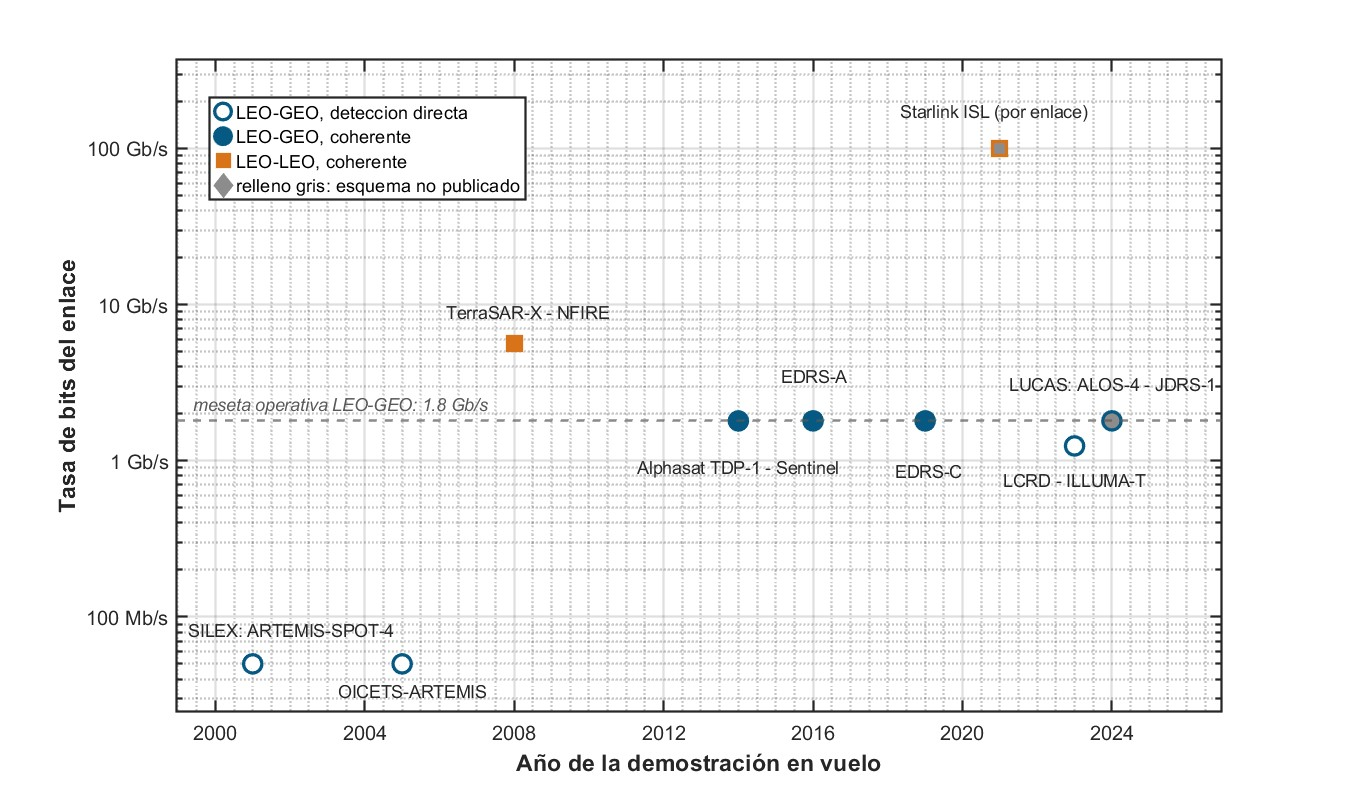
\includegraphics[width=\linewidth]{EvolucionTemporalEnlaceOptico}
  \caption[Evoluci\'on de los enlaces \'opticos inter-satelitales]{%
    Tasa de bits de los enlaces \'opticos inter-satelitales demostrados en
    vuelo. La forma del marcador indica el tipo de enlace (c\'irculo:
    LEO--GEO; cuadrado: LEO--LEO) y el relleno muestra el esquema de recepci\'on
    (hueco: sin oscilador local; lleno: coherente; gris: no publicado).
    Los enlaces LEO--GEO operativos permanecen en
    \SI{1.8}{\giga\bit\per\second} desde 2014, mientras las constelaciones
    comerciales LEO--LEO ya operan casi dos \'ordenes de magnitud por encima.
    Elaboraci\'on propia a partir de
    \cite{tolkernielsen2002,esa_silex2001,eoportal_artemis,esa_oicets2005,%
    smutny2009,tesat2018,esa_edrs,nasa_lcrd_illumat,nec_lucas2025,%
    chaudhry2021,starlink2024}.}
  \label{fig:evolucion-isl}
\end{figure}

En 2001 el experimento SILEX estableci\'o el primer enlace \'optico entre un
sat\'elite LEO y uno geoestacionario, entre SPOT-4 y ARTEMIS, a
\SI{50}{\mega\bit\per\second} con portadora en la banda de
\SIrange{800}{850}{\nano\metre} y fotodiodos de avalancha de
silicio~\cite{tolkernielsen2002,esa_silex2001}. El enlace entre OICETS/Kirari y
ARTEMIS, en 2005, repiti\'o exactamente la misma tasa en el sentido LEO hacia
GEO~\cite{eoportal_artemis,esa_oicets2005}. Cuatro a\~nos sin ganancia de
capacidad.

En 2008 los terminales LCT de Tesat enlazaron TerraSAR-X con NFIRE a
\SI{5.625}{\giga\bit\per\second} mediante recepci\'on homodina BPSK a
\SI{1064}{\nano\metre}~\cite{smutny2009,tesat2018}. Dos \'ordenes de magnitud
por encima de SILEX, sin un aumento del tama\~no de las \'opticas. Esta misma
familia de terminales es la que la Agencia Espacial Europea llev\'o a
operaci\'on en el sistema EDRS, primero como demostraci\'on entre Alphasat
TDP-1 y Sentinel-1A en 2014. Entr\'o en servicio con EDRS-A en 2016 y con
EDRS-C en 2019, siempre a \SI{1.8}{\giga\bit\per\second}~\cite{esa_edrs}.

En 2023 el par LCRD--ILLUMA-T cerr\'o el primer sistema de retransmisi\'on
\'optica bidireccional extremo a extremo de la NASA, entre la Estaci\'on
Espacial Internacional y un sat\'elite geoestacionario, a
\SI{1.2}{\giga\bit\per\second}~\cite{nasa_lcrd_illumat}. En 2024 el sistema
japon\'es LUCAS estableci\'o el enlace con DAICHI-4. En 2025 JAXA y NEC
reportaron la transmisi\'on de datos de misi\'on a
\SI{1.8}{\giga\bit\per\second} en banda de
\SI{1.5}{\micro\metre}~\cite{nec_lucas2025}. La presentaron como la
comunicaci\'on \'optica inter-satelital m\'as r\'apida del mundo, lo que fija
el estado del arte operativo en esa tasa. Diez a\~nos despu\'es de Alphasat, la
capacidad de un enlace LEO--GEO sigue siendo la misma.

El contraste con los enlaces LEO--LEO es grande. Starlink opera desde 2021 una
malla \'optica con capacidades del orden de \SI{100}{\giga\bit\per\second} por
enlace~\cite{chaudhry2021,starlink2024}, casi dos \'ordenes de magnitud por
encima del enlace de retransmisi\'on geoestacionario. La diferencia tiene dos
causas. En primer lugar se tiene el balance de potencia. Un enlace entre dos
sat\'elites LEO cubre unos pocos miles de kil\'ometros, mientras que un enlace
de retransmisi\'on geoestacionario cubre \SI{45000}{\kilo\metre}, lo que agrega
entre \num{19} y \SI{33}{\dB} de p\'erdida de espacio libre. Por otro lado
est\'a la forma en que se gestiona el programa. Un sistema de retransmisi\'on
GEO es un programa de interoperabilidad a quince a\~nos que congela una
generaci\'on de terminal, mientras que una constelaci\'on comercial renueva su
hardware cada pocos a\~nos.

La \cref{tab:capacidades} ordena estas capacidades por tecnolog\'ia de
transporte.

\begin{table}[htbp]
\centering
\begin{tabular}{llc}
\toprule
\textbf{Tecnolog\'ia} & \textbf{Fuente} & \textbf{Capacidad por enlace} \\
\midrule
Retransmisi\'on RF LEO--GEO, banda Ka         & \cite{nasa_katt}
                                     & $\sim$\SI{0.7}{\giga\bit\per\second} \\
Terminal \'optica comercial OOK-NRZ  & \cite{sda_oct,mynaric_condor}
                                     & \SIrange{0.31}{2.5}{\giga\bit\per\second} \\
Retransmisi\'on \'optica LEO--GEO en servicio & \cite{esa_edrs,nec_lucas2025}
                                     & \SI{1.8}{\giga\bit\per\second} \\
Malla \'optica LEO--LEO comercial    & \cite{starlink2024}
                                     & $\sim$\SI{100}{\giga\bit\per\second} \\
DP-QPSK coherente demostrado en tierra & \cite{scirep2022}
                                     & \SI{100}{\giga\bit\per\second} \\
\bottomrule
\end{tabular}
\caption[Capacidad por enlace seg\'un la tecnolog\'ia de transporte]{Capacidad
por enlace seg\'un la tecnolog\'ia de transporte. Valores representativos de
cada categor\'ia, no de cat\'alogo.}
\label{tab:capacidades}
\end{table}

De los enlaces inter-satelitales que operaron hasta hoy, todos los coherentes
pertenecen a la misma familia de terminales, con modulaci\'on binaria sobre una
\'unica polarizaci\'on. Hasta la fecha no se encontraron en la literatura
enlaces inter-satelitales operativos que empleen multiplexaci\'on en
polarizaci\'on. El est\'andar OCT de la SDA, que fija la interfaz de los
terminales comerciales actuales, especifica OOK-NRZ con un m\'aximo de
\SI{2.5}{\giga\bit\per\second}. Del transmisor no dice nada sobre
polarizaci\'on. Al receptor solo le pide que acepte cualquier estado de
polarizaci\'on recibido~\cite{sda_oct}. El formato de modulaci\'on que se
estudia en este trabajo ya se demostr\'o en enlaces \'opticos inal\'ambricos
terrestres. Por ejemplo, un enlace DP-QPSK de \SI{27.95}{\giga\baud} entre una
azotea y un dron, a velocidades angulares de seguimiento LEO, sostuvo
\SI{100}{\giga\bit\per\second}~\cite{scirep2022}.

Hasta la fecha, el incremento de la tasa de transmisi\'on en enlaces
satelitales apunt\'o a aumentar la tasa de s\'imbolo en modulaciones no
coherentes, combinado con la multiplexaci\'on en longitud de onda (WDM). Esta
es precisamente la direcci\'on que los programas en curso ya no pueden seguir.
Tanto el est\'andar OCT de la SDA como las especificaciones ESTOL de la ESA
apuntan a capacidades agregadas del orden del terabit por segundo. Subir solo
la tasa de s\'imbolo exigir\'ia anchos de banda y consumos incompatibles con
una plataforma LEO. Multiplexar en longitud de onda es el otro eje disponible.
El propio est\'andar OCT ya define \num{44} canales en banda
C~\cite{sda_oct}. Pero cada canal que se agrega conlleva sumar un l\'aser, un
amplificador y un terminal m\'as caro. El camino que queda es el que la
comunicaci\'on por fibra \'optica recorri\'o hace quince a\~nos. Pasar de
modulaci\'on binaria a formatos multinivel multiplexados en las dos
polarizaciones. La complejidad que eso agrega se absorbe en procesamiento
digital.

En este contexto, el trabajo desarrollado en este Proyecto Integrador aborda la
primera etapa del camino, con el estudio de un receptor \'optico coherente
DP-QPSK para un enlace LEO--GEO.

\section{Definici\'on del problema}
\label{sec:intro-problema}

Para pasar de \SI{10}{\giga\bit\per\second} a m\'as de
\SI{100}{\giga\bit\per\second} no alcanza con subir la potencia. Se necesita
multiplexar en polarizaci\'on y usar formatos de fase multinivel. Esto exige
detecci\'on coherente con procesamiento digital de la se\~nal recibida.

Hay tres motivos principales que sustentan la elecci\'on de un enlace \'optico
coherente para comunicaciones entre sat\'elites:

\begin{enumerate}
  \item \textbf{Espectro:} El espectro de RF est\'a saturado y requiere
        licencia, coordinaci\'on y control de interferencia. Las frecuencias
        \'opticas no est\'an sujetas a ese r\'egimen.
  \item \textbf{Directividad del haz:} A frecuencias \'opticas la divergencia
        del haz es del orden de los microradianes, lo que permite reducir la
        interferencia con otros sat\'elites y dificultar la intercepci\'on.
  \item \textbf{Masa y consumo:} Aperturas de cent\'imetros en lugar de metros.
        Por ejemplo, una antena de RF en banda Ka necesitar\'ia decenas de
        metros para el mismo balance de potencia, seg\'un la
        \cref{sec:canal-geometria}.
\end{enumerate}

La detecci\'on coherente con procesamiento digital es una tecnolog\'ia madura y
ampliamente desplegada en los enlaces de fibra \'optica terrestres. Un enlace inter-satelital LEO--GEO, en cambio, impone condiciones
que no aparecen en una fibra. Se tienen presentes un desplazamiento Doppler de
varios \si{\giga\hertz} que var\'ia durante el pase, una rotaci\'on continua
del estado de polarizaci\'on y una OSNR limitada por las enormes p\'erdidas de
potencia en el canal. Estas son las condiciones que el receptor tiene que
tolerar antes de poder garantizar la viabilidad del enlace. Por esto, la pregunta que este trabajo
se propone abordar es la siguiente.

\begin{quote}
\emph{\textquestiondown Puede un receptor coherente DP-QPSK de
\SI{128}{\giga\bit\per\second} estimar y compensar las degradaciones propias de
un enlace LEO--GEO, de forma que se obtenga una BER pre-FEC por
debajo del umbral que un c\'odigo de bloque de decisi\'on dura (HD) necesita para
cerrar el enlace?}
\end{quote}

\section{Objetivos, alcances y limitaciones}
\label{sec:intro-objetivos}

\subsection*{Objetivo general}

Desarrollar y validar, mediante simulaciones num\'ericas e implementaci\'on
experimental, un receptor \'optico coherente a tasas de hasta
\SI{128}{\giga\bit\per\second} que emplee modulaci\'on QPSK en doble
polarizaci\'on (DP-QPSK) para un enlace inter-satelital LEO--GEO, y evaluar su
desempe\~no frente a las degradaciones del canal espacial.

\subsection*{Objetivos espec\'ificos}

\begin{enumerate}
  \item Implementar modelos matem\'aticos de la cadena completa, con el
        transmisor, el canal satelital y el receptor coherente.
  \item Implementar los algoritmos de procesamiento digital necesarios en el
        receptor: ortogonalizaci\'on, recuperaci\'on de frecuencia y de reloj,
        ecualizaci\'on adaptativa MIMO y recuperaci\'on de fase.
  \item Desarrollar el balance de potencia y determinar la OSNR disponible en
        un enlace con p\'erdidas compatibles con las de un enlace LEO--GEO.
  \item Evaluar la tolerancia del receptor al Doppler, a la rotaci\'on del
        estado de polarizaci\'on y al ruido del l\'aser.
  \item Validar experimentalmente el procesamiento sobre capturas de laboratorio.
\end{enumerate}

\subsection*{Alcances y limitaciones}

Se modela un enlace \'optico coherente inter-satelital LEO--GEO de
aproximadamente \SI{45000}{\kilo\metre}, con transmisi\'on en la banda C
(\SIrange{1530}{1565}{\nano\metre}) y portadora en \SI{1550}{\nano\metre},
equivalente a \SI{193.4}{\tera\hertz}. La se\~nal es DP-QPSK, con
\SI{2}{\bit} por s\'imbolo en cada una de las dos polarizaciones. La tasa de
dise\~no es \SI{32}{\giga\baud}, y se evaluaron adem\'as
\SI{12.5}{\giga\baud} y \SI{25}{\giga\baud}.s

Quedan fuera del alcance la adquisici\'on y el seguimiento del haz (PAT), la
codificaci\'on FEC, de modo que se reporta BER pre-FEC contra el umbral HD-FEC
del \SI{7}{\percent} ($3{,}8\times10^{-3}$), y la retransmisi\'on, ya que se
modela solo el terminal receptor y no un retransmisor transparente.

\section{Organizaci\'on de la tesis}
\label{sec:intro-organizacion}

\begin{itemize}
  \item \Cref{cap:coherentes}: se presentan los fundamentos de la detecci\'on
        coherente y se fijan las m\'etricas del trabajo, es decir la relaci\'on
        entre la OSNR y la relaci\'on se\~nal a ruido por s\'imbolo, el EVM y
        la BER pre-FEC contra el umbral HD-FEC.

  \item \Cref{cap:canal}: se modela el canal LEO--GEO. Se calcula la p\'erdida
        del enlace a \SI{45000}{\kilo\metre}, el offset Doppler y su
        variaci\'on durante el pase, y la rotaci\'on del estado de
        polarizaci\'on.

  \item \Cref{cap:transceptor}: se modelan el transmisor y el receptor
        coherente, incluyendo los l\'aseres, el modulador, el front end y el
        ADC.

  \item \Cref{cap:dsp}: se describe la cadena de procesamiento digital bloque
        por bloque, profundizando en la recuperaci\'on de frecuencia, que es la
        que fija el l\'imite de captura del receptor.

  \item \Cref{cap:enlace}: se unen los tres anteriores en el balance de
        potencia. Se obtiene la OSNR disponible en el peor instante del pase y
        se la compara con la que necesita el receptor simulado para llegar al
        umbral HD-FEC.

  \item \Cref{cap:tolerancias}: se estudian los efectos de cada deterioro sobre
        el receptor, se identifica el mecanismo que fija su l\'imite y se
        contrasta ese l\'imite con el valor que impone el enlace.

  \item \Cref{cap:experimental}: se implementa la cadena en el laboratorio y se
        procesan capturas reales con el mismo DSP, para tres tasas de
        s\'imbolo.

  \item \Cref{cap:conclusiones}: se re\'unen las conclusiones, se resumen los
        aportes del trabajo y se propone la continuaci\'on.

\end{itemize}

% !TeX root = ../main.tex

\chapter{Fundamentos de comunicaciones \'opticas coherentes}
\label{cap:coherentes}

\section{Introducci\'on}
\label{sec:coh-intro}

En este cap\'itulo se re\'unen los fundamentos que utiliza el resto del trabajo. Primero
se describe la cadena óptica. Luego se explica el formato
DP-QPSK, c\'omo funciona la detecci\'on coherente y qu\'e hace el procesamiento
digital con las señales provenientes del front-end. Finalmente, se especifican las m\'etricas utilizadas, es decir la
relaci\'on entre la OSNR del balance de potencia y la relaci\'on se\~nal-ruido
en el punto de decisi\'on, el umbral HD-FEC contra el que se compara todo resultado y el EVM.

\section{El enlace \'optico coherente}
\label{sec:coh-enlace}

Un enlace \'optico coherente se separa en cuatro bloques, como muestra la
\Cref{fig:enlace-panorama}. El transmisor genera los s\'imbolos y modula la portadora con ellos. Esta se\~nal viaja a trav\'es del canal, degrad\'andose en el camino. El receptor
coherente bate la se\~nal contra un oscilador local y la lleva a banda base. El procesamiento digital tiene como objetivo deshacer estas degradaciones del canal, al igual que las provocadas por el equipo transmisor y receptor.

\begin{figure}[H]
  \centering
  \begin{tikzpicture}[
    font=\footnotesize,
    bloque/.style={draw, rounded corners=2pt, align=center,
                   minimum height=4.4em, text width=7.6em, inner sep=3pt},
    flecha/.style={-{Latex[length=2mm]}, thick}
  ]
    \node[bloque] (tx)
      {\textbf{Transmisor}\\[2pt]\scriptsize s\'imbolos, l\'aser, modulador\\[-1pt]%
       \scriptsize DP-IQ};
    \node[bloque, right=1.4em of tx] (ch)
      {\textbf{Canal LEO--GEO}\\[2pt]\scriptsize p\'erdidas, Doppler,\\[-1pt]%
       \scriptsize rotaci\'on de SOP};
    \node[bloque, right=1.4em of ch] (rx)
      {\textbf{Receptor coherente}\\[2pt]\scriptsize l\'aser LO, h\'ibrido\\[-1pt]%
       \scriptsize de \SI{90}{\degree}, ADC};
    \node[bloque, right=1.4em of rx] (dsp)
      {\textbf{DSP}\\[2pt]\scriptsize bloques\\[-1pt]%
       \scriptsize de compensaci\'on};

    \draw[flecha] (tx) -- (ch);
    \draw[flecha] (ch) -- (rx);
    \draw[flecha] (rx) -- (dsp);
  \end{tikzpicture}
  \caption[Esquema del enlace \'optico coherente]{%
    Los cuatro bloques de un enlace \'optico coherente. El canal se modela en
    el \cref{cap:canal}, el transmisor y el receptor en el
    \cref{cap:transceptor}, y el procesamiento digital en el \cref{cap:dsp}.}
  \label{fig:enlace-panorama}
\end{figure}

Cada bloque se desarrolla en detalle m\'as adelante, en el
cap\'itulo que le corresponde.

\section{Formato DP-QPSK}
\label{sec:coh-dpqpsk}

QPSK transmite dos bits por s\'imbolo en cuatro fases equiespaciadas. Con mapeo
Gray, los s\'imbolos vecinos difieren en un \'unico bit
(\cref{fig:constelacion}a), de modo que el error m\'as probable cuesta un solo
bit. La probabilidad de error de bit resulta
\begin{equation}
  \BER_{\mathrm{QPSK}} = \Qfun\!\left(\sqrt{2\,\EbNo}\right)
                       = \Qfun\!\left(\sqrt{\EsNo}\right),
  \label{eq:ber-qpsk}
\end{equation}
donde la segunda igualdad usa $E_s = 2E_b$.

\begin{figure}[H]
  \centering
  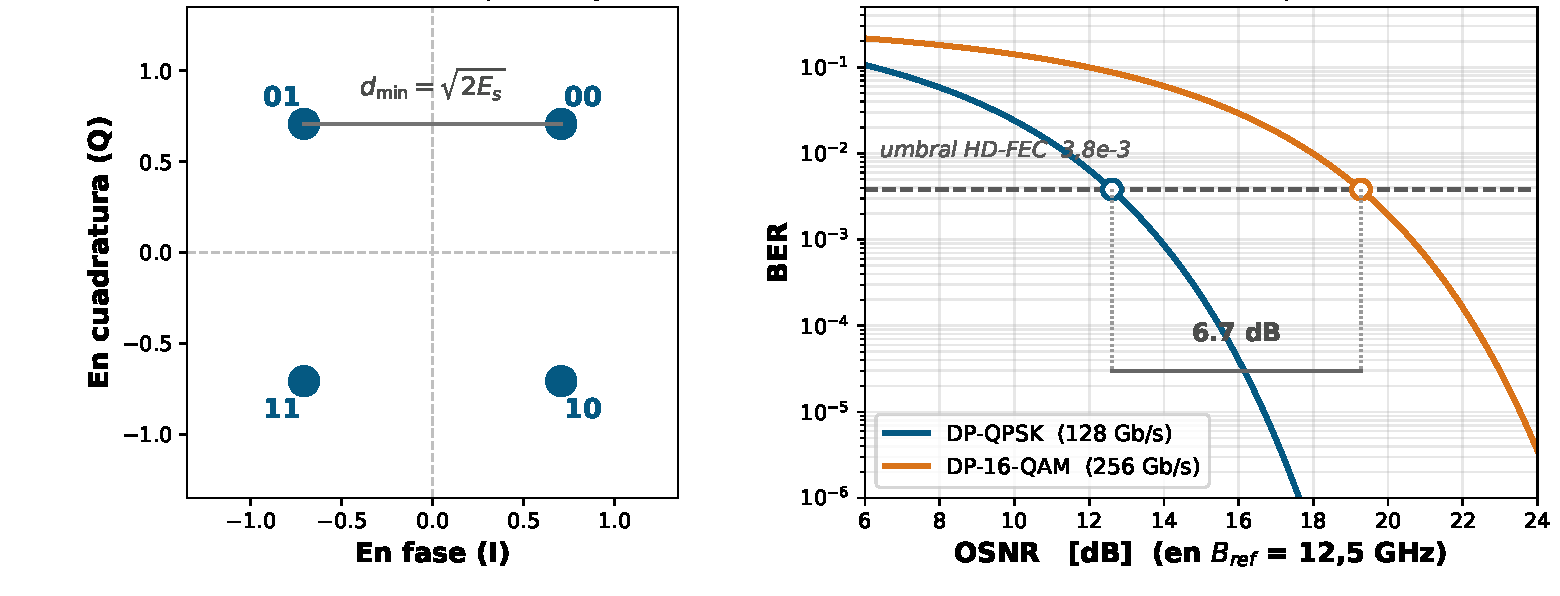
\includegraphics[width=\linewidth]{constelacion-qpsk}
  \caption[Constelaci\'on QPSK y elecci\'on del formato]{%
    (a)~Constelaci\'on QPSK con mapeo Gray. (b)~BER te\'orica contra OSNR a
    igual tasa de s\'imbolo (\SI{32}{\giga\baud}) y con las dos
    polarizaciones, para DP-QPSK y para 16-QAM. La comparaci\'on entre las dos
    se discute en la \cref{sec:coh-eleccion}.}
  \label{fig:constelacion}
\end{figure}

La multiplexaci\'on en polarizaci\'on (DP) duplica la tasa de bits sin
ensanchar el espectro, al transmitir dos secuencias QPSK independientes sobre
los dos modos ortogonales de polarizaci\'on de la misma portadora. A
\SI{32}{\giga\baud} con dos bits por s\'imbolo y dos polarizaciones se llega a
los \SI{128}{\giga\bit\per\second} de este trabajo.

Esto tiene dos costos. Por un lado, la potencia de transmisi\'on se reparte entre las dos
secuencias. Y por otro, el canal, que rota la polarizaci\'on de manera arbitraria y
variable, las mezcla, por lo que el receptor necesita un ecualizador MIMO
$2\times2$ que las vuelva a separar.

\section{Detecci\'on coherente}
\label{sec:coh-deteccion}

Para recuperar la informaci\'on de amplitud y fase presente en la portadora
\'optica hace falta un esquema de detecci\'on coherente. Un receptor de
detecci\'on directa mide $\abs{E_r}^2$, donde $E_r$ es el campo recibido, perdiendo la informaci\'on de la fase. La detecci\'on coherente consiste en hacer interferir la se\~nal recibida
contra un l\'aser oscilador local (LO) siguiendo la estructura de la
\Cref{fig:frontend}, conservando el campo completo. Como resultado, se habilitan
los formatos de modulaci\'on en amplitud y fase.

\begin{figure}[H]
  \centering
  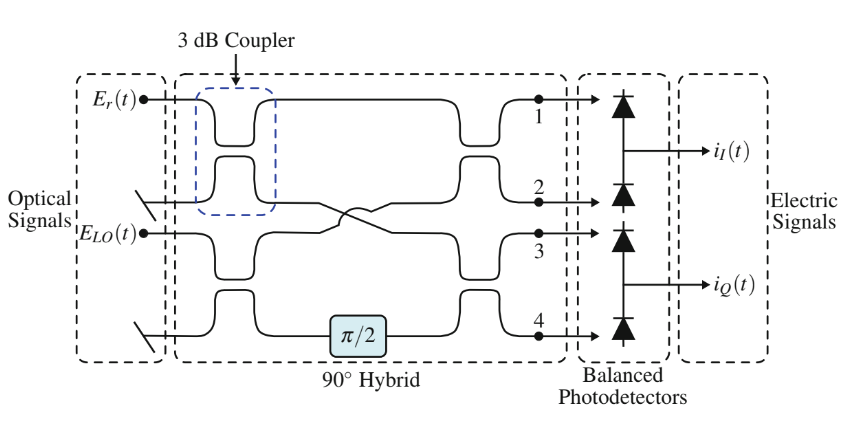
\includegraphics[width=0.86\linewidth]{FrontEndOpticoLibro}
  \caption[Front end \'optico coherente]{%
    Front end \'optico coherente de una polarizaci\'on: h\'ibrido de
    \SI{90}{\degree} formado por acopladores de \SI{3}{\dB} y dos pares de
    fotodetectores balanceados. Tomado de~\cite{mello2021}.}
  \label{fig:frontend}
\end{figure}

El bloque elemental es el acoplador de \SI{3}{\dB}, cuya matriz de
transferencia es
\begin{equation}
  \tilde{H}_c = \frac{1}{\sqrt{2}}
  \begin{bmatrix} 1 & 1 \\ 1 & -1 \end{bmatrix}.
  \label{eq:acoplador}
\end{equation}

Cuatro acopladores y un desfasaje de $\pi/2$ en una rama forman el h\'ibrido de
\SI{90}{\degree} de la \cref{fig:frontend}. Con $E_{LO}$ el campo del
oscilador local, los cuatro campos de salida resultan
\begin{equation}
  E_{1,2} = \tfrac{1}{2}\left(E_r \pm E_{LO}\right),
  \qquad
  E_{3,4} = \tfrac{1}{2}\left(E_r \pm j\,E_{LO}\right).
  \label{eq:hibrido}
\end{equation}

Cada par se detecta en configuraci\'on balanceada, es decir restando las dos
fotocorrientes,
\begin{equation}
  i_I(t) = i_1 - i_2 = R\abs{E_1}^2 - R\abs{E_2}^2,
  \qquad
  i_Q(t) = i_3 - i_4 = R\abs{E_3}^2 - R\abs{E_4}^2,
  \label{eq:balanceado}
\end{equation}
donde $R$ es la responsividad de los fotodiodos. Al utilizar fotodetectores
balanceados, los t\'erminos de detecci\'on directa $\abs{E_r}^2$ y
$\abs{E_{LO}}^2$ aparecen con el mismo signo y se cancelan, quedando
\'unicamente el batido entre se\~nal y oscilador local. Escribiendo
$E_r = A_r e^{j(\omega_s t + \phi_r)}$ y $E_{LO} = A_{LO} e^{j\omega_{LO} t}$,
\begin{align}
  i_I(t) &= A_r A_{LO} R\;\Re\!\left\{e^{\,j[\phi_r(t)+\omega_{IF}t]}\right\}
          = A_r A_{LO} R\cos\!\left(\phi_r(t)+\omega_{IF}t\right),
          \label{eq:iI}\\[2pt]
  i_Q(t) &= A_r A_{LO} R\;\Re\!\left\{e^{\,j[\phi_r(t)+\omega_{IF}t-\pi/2]}\right\}
          = A_r A_{LO} R\sin\!\left(\phi_r(t)+\omega_{IF}t\right),
          \label{eq:iQ}
\end{align}
con $\omega_{IF} = \omega_s - \omega_{LO}$ la frecuencia intermedia. Las dos
cuadraturas se combinan en una \'unica se\~nal compleja en banda base
equivalente,
\begin{equation}
  i(t) = i_I(t) + j\,i_Q(t) = R\,A_r A_{LO}\, e^{\,j[\phi_r(t)+\omega_{IF}t]},
  \label{eq:banda-base}
\end{equation}
que es la entrada del DSP luego del muestreo.

En~\eqref{eq:banda-base} se observa que la se\~nal \'util aumenta con $A_{LO}$.
Un oscilador local fuerte amplifica el batido sin amplificar el ruido
t\'ermico del amplificador de transimpedancia, de modo que el receptor, en
ausencia de un pre-amplificador \'optico, queda limitado por el ruido de
disparo del propio LO.

Cualquier desalineaci\'on entre las frecuencias de los dos l\'aseres,
incluyendo el corrimiento Doppler del enlace, aparece directamente como el
t\'ermino $\omega_{IF}t$. Es una rampa de fase que el procesamiento digital
debe estimar y eliminar antes de decidir sobre el s\'imbolo. De esa
estimaci\'on se encarga el bloque de recuperaci\'on de frecuencia, que se
desarrolla en el \cref{cap:dsp}. Su rango de captura es uno de los l\'imites
que mide el \cref{cap:tolerancias}.

\section{DSP del receptor}
\label{sec:coh-dsp-panorama}

La se\~nal que entrega el front end en la ecuaci\'on~\eqref{eq:banda-base}
tiene las cuadraturas desbalanceadas, una rampa de fase por el offset de
frecuencia, las dos polarizaciones mezcladas, y est\'a muestreada con una fase
de reloj incorrecta. El DSP deshace esas degradaciones a trav\'es de la cadena
de la \cref{fig:dsp-panorama}.

\begin{figure}[H]
  \centering
  \begin{tikzpicture}[
    font=\footnotesize,
    bloque/.style={draw, rounded corners=2pt, align=center,
                   minimum height=3.1em, text width=6.6em, inner sep=2pt},
    flecha/.style={-{Latex[length=2mm]}, thick}
  ]
    \node[bloque] (adc) {ADC\\[1pt]\scriptsize 2 muestras\\[-1pt]\scriptsize por s\'imbolo};
    \node[bloque, right=0.9em of adc]  (gsop) {Ortogonalizaci\'on\\[1pt]\scriptsize GSOP};
    \node[bloque, right=0.9em of gsop] (foc)  {Recuperaci\'on de frecuencia};
    \node[bloque, right=0.9em of foc]  (mf)   {Filtro adaptado\\[1pt]\scriptsize RRC};

    \node[bloque, below=3.0em of adc]  (clk)  {Recuperaci\'on de reloj};
    \node[bloque, right=0.9em of clk]  (eq)   {Ecualizador MIMO $2\times2$\\[1pt]\scriptsize DDLMS};
    \node[bloque, right=0.9em of eq]   (cpr)  {Recuperaci\'on de fase};
    \node[bloque, right=0.9em of cpr]  (dec)  {Decisi\'on\\[1pt]\scriptsize EVM y BER};

    \draw[flecha] (adc)  -- (gsop);
    \draw[flecha] (gsop) -- (foc);
    \draw[flecha] (foc)  -- (mf);
    \draw[flecha] (clk)  -- (eq);
    \draw[flecha] (eq)   -- (cpr);
    \draw[flecha] (cpr)  -- (dec);

    \coordinate (bajada) at ($(mf.south)+(0,-1.05em)$);
    \draw[flecha] (mf.south) -- (bajada) -| (clk.north);
  \end{tikzpicture}
  \caption[Cadena de procesamiento digital del receptor]{%
    DSP. En la implementaci\'on de este trabajo el ecualizador MIMO y la
    recuperaci\'on de fase est\'an integrados. Son dos lazos adaptativos
    distintos que operan sobre las mismas muestras.}
  \label{fig:dsp-panorama}
\end{figure}

Cada bloque se encarga de una degradaci\'on concreta:

\begin{itemize}\itemsep2pt
  \item \textbf{Ortogonalizaci\'on (GSOP):} Se encarga de corregir el
        desbalance de ganancia y de cuadratura entre las componentes I y Q que
        introducen el h\'ibrido y los fotodetectores.
  \item \textbf{Recuperaci\'on de frecuencia:} Estima y quita el t\'ermino
        $\omega_{IF}$ de la ecuaci\'on~\eqref{eq:banda-base}, que en este
        enlace est\'a dominado por el Doppler.
  \item \textbf{Filtro adaptado:} Aplica la mitad del coseno alzado que falta
        para completar el criterio de Nyquist y maximizar la relaci\'on
        se\~nal-ruido en el instante de muestreo.
  \item \textbf{Recuperaci\'on de reloj:} Corrige el error de frecuencia y de
        fase de muestreo respecto del reloj del transmisor.
  \item \textbf{Ecualizador MIMO $2\times2$:} Invierte la matriz de Jones del
        canal y separa las dos polarizaciones. Sigue adem\'as su rotaci\'on a
        lo largo del pase.
  \item \textbf{Recuperaci\'on de fase:} Cancela el ruido de fase de los
        l\'aseres y el error de frecuencia residual.
  \item \textbf{Decisi\'on:} Mapea cada s\'imbolo al punto m\'as cercano de la
        constelaci\'on, y calcula EVM y BER.
\end{itemize}

La implementaci\'on de cada bloque, con sus par\'ametros y sus l\'imites de
operaci\'on, se desarrolla en el \cref{cap:dsp}.

\section{M\'etricas de desempe\~no}
\label{sec:coh-metricas}

\subsection{OSNR y relaci\'on se\~nal-ruido}
\label{sec:coh-osnr}

El balance de potencia del enlace se expresa en OSNR, medida en un ancho de
banda de referencia convencional $\Bref = \SI{12.5}{\giga\hertz}$
(\SI{0.1}{\nano\metre} en banda C). La detecci\'on, en cambio, depende de la
relaci\'on se\~nal-ruido. La conversi\'on entre ambas es
\begin{equation}
  \EsNo\,[\si{\dB}] = \OSNR\,[\si{\dB}] + 10\log_{10}\!\frac{\Bref}{\Rs}.
  \label{eq:osnr-esno}
\end{equation}
A \SI{32}{\giga\baud} el segundo t\'ermino vale \SI{-4.08}{\dB}.

La diferencia entre las dos es el ancho de banda sobre el que se integra el
ruido. El de referencia est\'a fijo, mientras que el del punto de decisi\'on sigue a la
tasa de s\'imbolo. Por eso la OSNR describe al canal y la relaci\'on
se\~nal-ruido describe lo que necesita el receptor.

\subsection{El umbral HD-FEC}
\label{sec:coh-fec}

Los sistemas de comunicaciones se dise\~nan para operar por debajo de un umbral
pre-FEC que un c\'odigo de correcci\'on posterior lleva a una BER de salida
mucho m\'as baja. Este trabajo adopta el umbral cl\'asico de decisi\'on dura
(HD-FEC) con \SI{7}{\percent} de \emph{overhead},
$\BER = 3{,}8\times10^{-3}$, correspondiente al c\'odigo de bloque del
ap\'endice~I.9 de la recomendaci\'on ITU-T G.975.1~\cite{itu_g975}, que lleva
la entrada a una tasa de errores de menos de $10^{-13}$ a la salida.

Combinando \eqref{eq:ber-qpsk} y \eqref{eq:osnr-esno}, ese umbral requiere
$\EbNo = \SI{5.52}{\dB}$, equivalente a $\EsNo = \SI{8.53}{\dB}$ y a
$\OSNR = \SI{12.61}{\dB}$ te\'oricos. Este valor es el punto de comparaci\'on
de todos los barridos del \cref{cap:tolerancias}. La diferencia entre la OSNR
simulada y los \SI{12.61}{\dB} es la penalidad de implementaci\'on del
receptor.

Adoptar un umbral fijo permite reducir todo el desempe\~no del enlace a una
sola pregunta binaria por cada condici\'on de canal. Si la BER pre-FEC queda
por debajo de $3{,}8\times10^{-3}$, entonces el sistema funciona.

\subsection{Estimaci\'on de la BER mediante el EVM}
\label{sec:coh-evm}

La magnitud del vector de error (EVM) mide la dispersi\'on de los s\'imbolos
recibidos alrededor de sus posiciones ideales. Se define como la ra\'iz del
error cuadr\'atico medio respecto de la referencia, normalizado a la potencia
media de la constelaci\'on,
\begin{equation}
  \EVM = \sqrt{\frac{\E{\abs{r_k - s_k}^2}}{\E{\abs{s_k}^2}}},
  \label{eq:evm}
\end{equation}
donde $r_k$ es el s\'imbolo recibido y $s_k$ el transmitido.

Para una constelaci\'on de energ\'ia constante como QPSK, y bajo la
hip\'otesis de ruido gaussiano complejo, el EVM es directamente el inverso de
la ra\'iz de la relaci\'on se\~nal-ruido, y la BER se estima como
\begin{equation}
  \EVM_{\mathrm{rms}}^{2} \simeq \frac{1}{\mathrm{SNR}},
  \qquad
  \BER \simeq \Qfun\!\left(\frac{1}{\EVM_{\mathrm{rms}}}\right).
  \label{eq:evm-ber}
\end{equation}

La consistencia de \eqref{eq:evm-ber} con el umbral HD-FEC se comprueba
directamente, ya que $\Qfun(1/0{,}3746) = 3{,}80\times10^{-3}$. Es decir,
$\EVM = \SI{37.46}{\percent}$ es el umbral HD-FEC expresado como EVM, y las dos
m\'etricas son intercambiables mientras el ruido dominante sea gaussiano.



\subsection{Estimaci\'on de la BER por conteo de errores}
\label{sec:coh-conteo}

La BER contada tiene un piso que no depende del receptor sino del largo de la
simulaci\'on. Si sobre $N$ bits no se observa ning\'un error, la regla de tres
establece que el intervalo de confianza del \SI{95}{\percent} para la
probabilidad de error tiene cota superior
\begin{equation}
  \BER_{\min} = \frac{3}{N}.
  \label{eq:piso-conteo}
\end{equation}
Con $N_{\mathrm{symb}} = 3\times10^{5}$ s\'imbolos por polarizaci\'on, el piso
est\'a en el orden de $5\times10^{-6}$, lo que implica una cota m\'axima de
OSNR que se puede analizar.

El EVM no tiene este problema. Se calcula sobre todos los s\'imbolos, converge
con un n\'umero mucho menor de ellos y var\'ia de forma continua incluso donde
no hay errores. Por eso, en los barridos de tolerancia del
\cref{cap:tolerancias} la m\'etrica principal es el EVM y la BER que se reporta
es la estimada mediante \eqref{eq:evm-ber}. La BER contada se usa solo como
verificaci\'on, donde el n\'umero de errores es estad\'isticamente suficiente.

\section{Elecci\'on del formato}
\label{sec:coh-eleccion}

La alternativa para duplicar la tasa de bits es subir el orden de la
modulaci\'on en lugar de multiplexar en polarizaci\'on. Con las m\'etricas ya
definidas, las dos opciones se pueden comparar sobre el mismo eje. La
\cref{fig:constelacion}b muestra por qu\'e no se eligi\'o este camino.

A igual tasa de s\'imbolo, 16-QAM entrega \SI{256}{\giga\bit\per\second} pero
necesita \SI{19.3}{\dB} de OSNR para alcanzar el umbral HD-FEC, frente a los
\SI{12.6}{\dB} de DP-QPSK. Son \SI{6.7}{\dB} adicionales, o \SI{3.7}{\dB} si la
comparaci\'on se hace a igual tasa de bits, que un enlace limitado
por potencia puede ahorrarse.

Hay una segunda raz\'on. Al tener una separaci\'on angular menor y un nivel
m\'as en amplitud que QPSK, 16-QAM es bastante m\'as sensible al ruido de fase
y al RIN de los l\'aseres. DP-QPSK es entonces el formato que maximiza la tasa
de bits dentro del presupuesto de potencia disponible.

\section{Conclusiones}
\label{sec:coh-conclusiones}

El enlace se separa en transmisor, canal, receptor coherente y procesamiento
digital. Este cap\'itulo describi\'o los cuatro bloques a grandes rasgos, y cada uno
se retoma despu\'es en su propio cap\'itulo.

Con detecci\'on coherente se obtiene la informaci\'on de fase y de amplitud del
campo en banda base equivalente, ecuaci\'on~\eqref{eq:banda-base}, y con ella
la posibilidad de modular en amplitud, fase y polarizaci\'on. El precio es que
toda desalineaci\'on entre los dos l\'aseres queda integrada en la se\~nal como
una rampa de fase que el DSP debe deshacer.

El desempe\~no se reporta contra un \'unico umbral,
$\BER = 3{,}8\times10^{-3}$, equivalente a $\OSNR = \SI{12.61}{\dB}$
te\'oricos y a $\EVM = \SI{37.46}{\percent}$. La m\'etrica principal de los
barridos es el EVM, porque no tiene el piso de conteo $3/N$ que limita a la BER
por conteo de errores.

En base a este umbral, la tasa de \SI{32}{\giga\baud} con DP-QPSK es el punto de operaci\'on que
maximiza la tasa de bits dentro del presupuesto de potencia disponible.
% !TeX root = ../main.tex
%% =======================================================================
%  CAPITULO 3 — EL CANAL INTER-SATELITAL LEO-GEO

\chapter{El canal inter-satelital LEO--GEO}
\label{cap:canal}

\section{Introducci\'on}
\label{sec:canal-intro}

Un enlace \'optico en el vac\'io es muy diferente a uno de fibra \'optica. Al pasar del segundo al primero, desaparecen la
dispersi\'on crom\'atica, las no linealidades de Kerr y la atenuaci\'on
distribuida. A cambio aparecen otros tres efectos que la fibra no tiene: un
desplazamiento Doppler de varios \si{\giga\hertz} que var\'ia
durante el pase del sat\'elite, una rotaci\'on del estado de polarizaci\'on impuesta
por la actitud de las plataformas, y una OSNR fijada por
un balance de potencia a \SI{45000}{\kilo\metre}.

\begin{figure}[H]
  \centering
  \resizebox{\textwidth}{!}{%
  \begin{tikzpicture}[
    font=\footnotesize, >={Latex[length=2mm]},
    eq/.style ={draw=gray!70, dashed, rounded corners=3pt, fill=gray!10,
                align=center, minimum height=3.4em, text width=7.6em, inner sep=3pt},
    ch/.style ={draw=cyan!45!blue!60, rounded corners=3pt, fill=cyan!12,
                align=center, minimum height=3.4em, text width=7.6em, inner sep=3pt},
    fl/.style ={->, thick}
  ]
    \node[eq] (b)   {Booster \'optico (Tx)\\[1pt]$G_b=\SI{35}{\dB}$};
    \node[ch, right=1.1em of b]  (l) {P\'erdida del enlace\\[1pt]$L\simeq\SI{73}{\dB}$};
    \node[ch, right=1.1em of l]  (d) {Efecto Doppler\\[1pt]$E\to E\,e^{j\phi_D(t)}$};
    \node[ch, right=1.1em of d]  (s) {Rotaci\'on del SOP\\[1pt]$\mathbf{E}\to\mathbf{R}(\theta)\mathbf{E}$};
    \node[eq, right=1.1em of s]  (e) {Pre-amplificador\\[1pt]EDFA (Rx)};

    \draw[fl] ($(b.west)-(1.1em,0)$) -- (b.west);
    \draw[fl] (b) -- (l);  \draw[fl] (l) -- (d);
    \draw[fl] (d) -- (s);  \draw[fl] (s) -- (e);
    \draw[fl] (e.east) -- ++(1.1em,0);

    \node[above=0.2em of b.north west, anchor=south west, font=\scriptsize] {$E_{tx}(t)$};
    \node[above=0.2em of l.north west, anchor=south west, font=\scriptsize] {$E_{b}(t)$};
    \node[above=0.2em of d.north west, anchor=south west, font=\scriptsize] {$E_{att}(t)$};
    \node[above=0.2em of s.north west, anchor=south west, font=\scriptsize] {$E_{Dop}(t)$};
    \node[above=0.2em of e.north west, anchor=south west, font=\scriptsize] {$E_{rot}(t)$};
    \node[above=0.2em of e.north east, anchor=south east, font=\scriptsize] {$E_{rx}(t)$};
  \end{tikzpicture}}
  \caption[Modelo del canal inter-satelital]{%
    Modelo del canal implementado en la simulaci\'on. En trazo continuo, los
    tres bloques que son propiamente el canal. En trazo punteado, los dos
    amplificadores del terminal, que no forman parte del canal pero son la
    principal fuente de ruido del sistema y determinan la OSNR con la que
    llega la se\~nal al receptor. Los valores de ganancia y figura de ruido de
    los dos amplificadores se justifican en el \cref{cap:enlace}.}
  \label{fig:canal-cadena}
\end{figure}

La \cref{fig:canal-cadena} muestra c\'omo se model\'o la cadena. Este
cap\'itulo desarrolla cada bloque y termina con una tabla que re\'une los
par\'ametros del modelo. Las tolerancias del receptor frente a cada uno de
estos deterioros se miden en el \cref{cap:tolerancias}.

\section{Estimaci\'on de p\'erdidas del enlace}
\label{sec:canal-geometria}

La \cref{fig:geometria} plantea el problema. El sat\'elite LEO orbita a
\SI{550}{\kilo\metre} de altura con inclinaci\'on $i=\SI{98}{\degree}$, heliosincr\'onica (la \'orbita habitual de una constelaci\'on de
observaci\'on), y el sat\'elite GEO est\'a en \'orbita geoestacionaria a
\SI{42164}{\kilo\metre} del centro de la Tierra. Durante el pase visible, es decir el intervalo de cada \'orbita en que los dos
sat\'elites se ven sin que la Tierra se interponga, la distancia entre ambos
var\'ia entre \SIrange{35267}{44255}{\kilo\metre}. Todo el balance de potencia de este
trabajo se calcula en el extremo superior de ese rango, redondeado a
$d = \SI{45000}{\kilo\metre}$. De esta manera, se garantiza que el enlace cierre en toda la
ventana visible, y no solo en su tramo central. 

\begin{figure}[H]
\centering
\begin{tikzpicture}[font=\small, >={Latex[length=2mm]}, scale=1.15]
\definecolor{cLEO}{RGB}{217,115,22}
\definecolor{cGEO}{RGB}{11,90,127}
\definecolor{cVR}{RGB}{190,30,45}

% Geometria, con la escala radial respetada
\fill[gray!35] (0,0) circle (0.75);
\draw[gray!60] (0,0) circle (0.75);
\node[font=\scriptsize, gray!40!black] at (0,-0.02) {Tierra};
\draw[cGEO, dashed, thick] (0,0) ellipse (4.96 and 1.50);
\draw[cLEO, thick] (0,0) ellipse (0.28 and 0.82);

% Posiciones sobre cada orbita
\coordinate (L) at (0.0486,0.8075);
\coordinate (G) at (4.66,0.51);

\draw[very thick] (L) -- (G);
\node[font=\footnotesize, above, sloped] at ($(L)!0.55!(G)$) {$R(t)$};

% Velocidades orbitales, tangentes a cada orbita en el punto dibujado
% (v_L a 0,08 unidades por km/s; v_G al doble, para que se vea)
\draw[->, cLEO, very thick] (L) -- ++(-0.540,0.279)
  node[above, font=\scriptsize] {$\mathbf{v}_L$};
\draw[->, cGEO, very thick] (G) -- ++(-0.376,0.314)
  node[above left=-1pt, font=\scriptsize] {$\mathbf{v}_G$};

\fill[cLEO] (L) circle (2.4pt);
\fill[cGEO] (G) circle (2.4pt);
\node[cGEO, below right=0pt and 1pt of G, font=\bfseries\footnotesize] {GEO};
\node[cLEO, font=\bfseries\footnotesize] at (0.42,1.04) {LEO};

\node[cLEO, font=\scriptsize, align=right, anchor=east] (etLEO) at (-1.3,-2.10)
  {\'orbita LEO\\ $h=\SI{550}{\kilo\metre}$};
\draw[cLEO!60, thin] (etLEO.east) -- (-0.19,-0.76);
\node[cGEO, font=\scriptsize, anchor=west] (etGEO) at (0.7,-2.10)
  {\'orbita GEO, $r=\SI{42164}{\kilo\metre}$};
\draw[cGEO!60, thin] (etGEO.north) -- (2.2,-1.35);

% Detalle en el LEO: vectores ampliados (0,42 unidades por km/s)
\draw[gray!55, rounded corners=3pt, fill=white] (-4.15,2.35) rectangle (-0.05,4.50);
\draw[gray!55, thin] (L) circle (0.16);
\draw[gray!55, thin] ($(L)+(-0.05,0.15)$) -- (-0.05,2.35);

\coordinate (O) at (-0.95,2.75);
\coordinate (Gd) at ($(O)+(G)-(L)$);   % direccion de la linea de vista

\draw[thick] (O) -- ($(O)!0.85cm!(Gd)$);
\draw[gray!70, thin, dashed] (O) -- ($(O)!-2.6cm!(Gd)$);

\coordinate (VL) at ($(O)+(-2.832,1.463)$);
\coordinate (VR) at ($(VL)+(0.989,-0.827)$);
\draw[->, cLEO, very thick] (O) -- (VL)
  node[pos=0.55, above right=-1pt, font=\scriptsize] {$\mathbf{v}_L$};
\draw[->, cGEO, very thick] (VL) -- (VR)
  node[pos=0.5, left=2pt, font=\scriptsize] {$-\mathbf{v}_G$};
\draw[->, very thick] (O) -- (VR)
  node[pos=0.45, above=0pt, font=\scriptsize] {$\mathbf{v}_\mathrm{rel}$};

\coordinate (P) at ($(O)!(VR)!(Gd)$);
\draw[gray!60!black, dashed] (VR) -- (P)
  node[pos=0.5, right=1pt, font=\scriptsize] {$v_\perp$};
\coordinate (a) at ($(P)!1.4mm!(O)$);
\coordinate (b) at ($(P)!1.4mm!(VR)$);
\draw[gray!60!black, thin] (a) -- ($(a)+(b)-(P)$) -- (b);
\draw[->, cVR, line width=1.5pt] (O) -- (P);
\node[cVR, font=\scriptsize, below] at ($(O)!0.5!(P)$) {$v_r$};
\fill[cLEO] (O) circle (2.2pt);
\end{tikzpicture}
\caption[Geometr\'ia del enlace LEO--GEO]{%
Geometr\'ia del enlace, con la escala radial respetada. Las velocidades
orbitales son tangentes a cada \'orbita. El recuadro ampl\'ia los vectores en
el LEO: la velocidad relativa $\mathbf{v}_\mathrm{rel}=\mathbf{v}_L-\mathbf{v}_G$
se descompone sobre la l\'inea de vista. Solo la componente $v_r=dR/dt$ cambia
la distancia y produce Doppler, $f_D=-v_r/\lambda$; la componente $v_\perp$
hace girar la l\'inea de vista. Durante el pase visible $R(t)$ recorre
\SIrange{35267}{44255}{\kilo\metre}.}
\label{fig:geometria}
\end{figure}
La p\'erdida de espacio libre y la ganancia de una antena de apertura circular son
\begin{equation}
  L_{0} = \left(\frac{4\pi d}{\lambda}\right)^{2},
  \qquad
  G = \left(\frac{\pi D}{\lambda}\right)^{2},
  \label{eq:fspl}
\end{equation}
donde $d$ es la distancia entre los dos terminales y $D$ el di\'ametro de la
apertura.

Con $d=\SI{45000}{\kilo\metre}$ y $\lambda=\SI{1550}{\nano\metre}$, la
p\'erdida de espacio libre vale \SI{291.24}{\dB}. El telescopio transmisor, de
di\'ametro $D_{tx}=\SI{135}{\milli\metre}$, aporta \SI{108.74}{\dB} de
ganancia. El receptor, de $D_{rx}=\SI{250}{\milli\metre}$, aporta
\SI{114.10}{\dB}. Los dos di\'ametros corresponden a terminales que ya
fueron desplegadas. El enlace LEO--GEO de EDRS usa telescopios de
\SI{135}{\milli\metre}~\cite{gutlich2014}, mientras que las terminales de SILEX, el primer
enlace \'optico LEO--GEO que oper\'o en \'orbita, usaban
\SI{250}{\milli\metre} en los dos extremos~\cite{carrascocasado2020,
esa_silex2001}. Suponiendo \SI{5}{\dB} de p\'erdida por error de apuntamiento,
la p\'erdida neta del enlace es
\begin{equation}
  L = L_{0} - G_{tx} - G_{rx} + L_{ap} = \SI{73.40}{\dB}.
  \label{eq:pathloss}
\end{equation}

Vi\'endolo en t\'erminos absolutos:
\begin{equation}
  \frac{L_{0}\,L_{ap}}{G_{tx}G_{rx}}
    = L_{ap}\left(\frac{4\,d\,\lambda}{\pi\,D_{tx}D_{rx}}\right)^{2}.
  \label{eq:pathloss-cerrada}
\end{equation}

La p\'erdida neta del enlace no crece con $1/\lambda^{2}$ sino que es
proporcional a $\lambda^{2}$, siempre que los di\'ametros de las dos aperturas
se mantengan fijos. Cuanto menor es la longitud de onda, menor es la
p\'erdida geom\'etrica del enlace. Esta es una de las ventajas principales de
las comunicaciones \'opticas frente a las de RF: permiten alcanzar una elevada directividad utilizando aperturas de dimensiones mucho menores. Por ejemplo, para conseguir el mismo
balance en banda Ka, con $\lambda\approx\SI{1}{\centi\metre}$, har\'ian falta
antenas unas \num{80} veces m\'as grandes en los dos extremos del enlace, del
orden de \SI{20}{\metre} en lugar de los \SI{250}{\milli\metre} del telescopio
\'optico.

La contraparte es la divergencia reducida del haz. Para un telescopio de
\SI{250}{\milli\metre} a \SI{1550}{\nano\metre} la divergencia es del orden de unos pocos
microradianes, lo que impone requisitos exigentes de precisi\'on al sistema de
adquisici\'on, apuntamiento y seguimiento. Por esa raz\'on se toma una
p\'erdida por apuntamiento de \SI{5}{\dB} en el balance del enlace.

\section{Efecto Doppler}
\label{sec:canal-doppler}

En un enlace de comunicaciones, el efecto Doppler introduce un desplazamiento
relativo $v_r/c$ com\'un a todas las componentes frecuenciales de la onda. Existen tres par\'ametros principales que derivan del efecto Doppler, estos son:
\begin{align}
  \Df    &= \frac{v_r}{\lambda}  &&\text{offset de portadora,}
           \label{eq:dop-offset}\\
  \fdot  &= \frac{a_r}{\lambda}  &&\text{tasa de variaci\'on (chirp),}
           \label{eq:dop-chirp}\\
  \delta &= \frac{v_r}{c}        &&\text{error de frecuencia de muestreo (SFO).}
           \label{eq:dop-sfo}
\end{align}
Ac\'a $v_r$ es la velocidad radial entre los dos sat\'elites, $a_r$ la
aceleraci\'on radial, $\lambda$ la longitud de onda y $c$ la velocidad de la
luz.

Los tres se obtuvieron de un modelo kepleriano de dos cuerpos con \'orbitas
circulares, barriendo la ascensi\'on recta del nodo ascendente para encontrar
la geometr\'ia m\'as desfavorable y descartando los instantes en que la l\'inea
de vista atraviesa la Tierra. La velocidad radial y su derivada se calculan en
forma cerrada a trav\'es de las siguientes expresiones~\cite{vallado2013},
\begin{equation}
  v_r = \frac{\Delta\mathbf{r}\cdot\Delta\mathbf{v}}{R},
  \qquad
  a_r = \frac{\lvert\Delta\mathbf{v}\rvert^{2}
             + \Delta\mathbf{r}\cdot\Delta\mathbf{a} - v_r^{2}}{R},
  \label{eq:rangerate}
\end{equation}
donde $\Delta\mathbf{r}$, $\Delta\mathbf{v}$ y $\Delta\mathbf{a}$ son la
posici\'on, la velocidad y la aceleraci\'on del sat\'elite GEO relativas al
LEO. El escalar $R$ es el m\'odulo de $\Delta\mathbf{r}$, o sea la distancia
instant\'anea entre los dos. 

\begin{figure}[H]
  \centering
  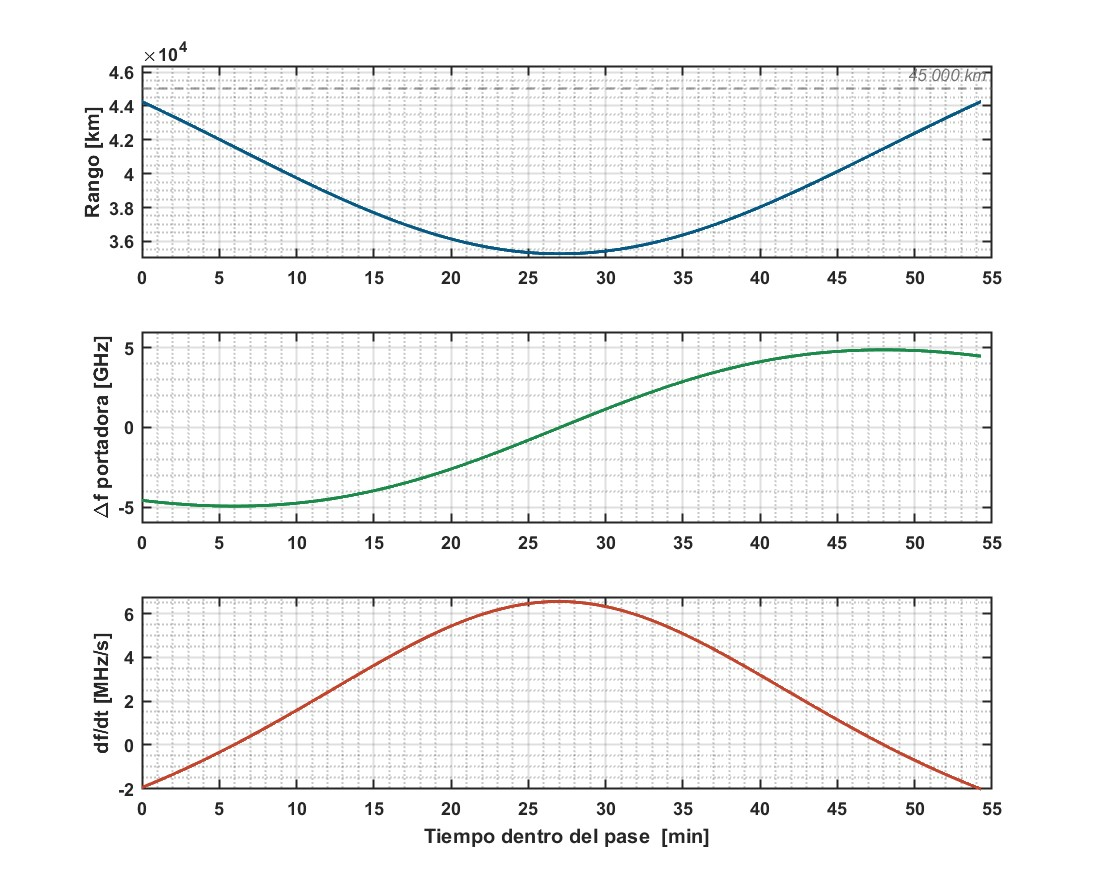
\includegraphics[width=0.94\linewidth]{DopplerGeometria}
  \caption[Doppler a lo largo de un pase LEO--GEO]{%
    Peor geometr\'ia del enlace LEO--GEO. El offset de portadora no es un valor
    fijo: barre de $-4{,}94$ a $+\SI{4.94}{\giga\hertz}$ en los
    \SI{54.3}{\minute} que dura la ventana visible, y lo hace con una
    pendiente que llega a \SI{6.55}{\mega\hertz\per\second}.}
  \label{fig:pase-doppler}
\end{figure}

El resultado, en la peor geometr\'ia, es $v_r = \SI{7.66}{\kilo\metre\per\second}$
y $a_r = \SI{10.15}{\metre\per\second\squared}$, con una ventana visible de
\SI{54.3}{\minute} por \'orbita. Esto corresponde a:

\begin{itemize}\itemsep2pt
  \item \textbf{Offset de portadora} $\abs{\Df} = \SI{4.94}{\giga\hertz}$. Es
        uno de los deterioros m\'as nocivos del canal y el que fija el requisito de captura
        del recuperador de frecuencia.
  \item \textbf{Tasa Doppler} $\abs{\fdot} = \SI{6.55}{\mega\hertz\per\second}$.
        Se analiza su contribuci\'on en el \cref{cap:tolerancias}.
  \item \textbf{Error de reloj} $\delta = \SI{25.55}{\ppm}$, equivalente a
        \SI{818}{\kilo\hertz} sobre \SI{32}{\giga\baud}. En un bloque de
        \num{3e5} s\'imbolos el muestreo se desliza \num{7.7} s\'imbolos, de
        modo que el recuperador de reloj debe ser capaz de corregir estos
        errores.
\end{itemize}

\subsection*{Requisito de captura}



De la simulaci\'on de la secci\'on anterior se obtiene un offset m\'aximo de
\SI{4.94}{\giga\hertz} en la peor geometr\'ia del pase. Cabe notar que este valor se encuentra por debajo de la
cota que se obtiene suponiendo las dos velocidades orbitales antiparalelas y
alineadas con la l\'inea de vista, $v_L + v_G =
\SI{10.66}{\kilo\metre\per\second}$ o \SI{6.88}{\giga\hertz}, que es una
situaci\'on que la geometr\'ia orbital no permite.

A este valor hay que sumarle la incerteza de los l\'aseres. El recuperador de
frecuencia compensa la diferencia entre la portadora recibida y el oscilador
local. Cada l\'aser tiene su propio error absoluto frente a la grilla en la
que se lo sintoniza, y un m\'odulo comercial sintonizable especifica
\SI{\pm1.5}{\giga\hertz} de exactitud sobre toda la banda C ~\cite{ppcl500}. Esta es una cota de peor caso sobre temperatura y
envejecimiento. Entre dos unidades puestas en el mismo canal la diferencia
t\'ipica es una fracci\'on del valor, as\'i que se adopta
\SI{1}{\giga\hertz} de residuo, y el requisito de captura resulta
\begin{equation}
  \abs{\Df}_{\mathrm{req}}
    = \underbrace{\SI{4.94}{\giga\hertz}}_{\text{Doppler, peor geometr\'ia}}
    + \underbrace{\SI{1.00}{\giga\hertz}}_{\text{residuo de l\'aseres}}
    \simeq \SI{6.0}{\giga\hertz}.
  \label{eq:requisito-captura}
\end{equation}

De esta manera, se puede asegurar que si el sistema soporta estas frecuencias, el enlace es posible.

\section{Rotaci\'on del estado de polarizaci\'on}
\label{sec:canal-sop}

Los dos telescopios no comparten una
referencia de actitud com\'un, y el \'angulo entre sus planos de polarizaci\'on
cambia a lo largo del pase. Por esta raz\'on, se tiene una rotaci\'on de los ejes de polarizaci\'on que var\'ia en el tiempo. En el formalismo de Jones, el canal es una matriz
de rotaci\'on
\begin{equation}
  \mathbf{R}(\theta) =
  \begin{bmatrix} \cos\theta & -\sin\theta \\ \sin\theta & \cos\theta \end{bmatrix},
  \qquad
  \mathbf{E}_{\mathrm{out}} = \mathbf{R}(\theta(t))\,\mathbf{E}_{\mathrm{in}},
  \label{eq:jones}
\end{equation}
que mezcla las dos tributarias sin atenuarlas.

El \'angulo se model\'o como la suma de tres contribuciones,
\begin{equation}
  \theta(t) = \theta_{0} + \dot{\theta}\,t
            + \sum_{k} A_{k}\sin(2\pi f_{k} t + \phi_{k}),
  \label{eq:sop}
\end{equation}
con significado f\'isico distinto cada una:

\begin{itemize}\itemsep2pt
  \item $\theta_0$ es el desalineamiento inicial entre las dos terminales. El
        caso m\'as exigente para el demultiplexado es $\theta_0=\pi/4$, donde
        las dos polarizaciones llegan mezcladas por igual y el ecualizador no
        tiene ninguna asimetr\'ia de la que partir.
  \item $\dot\theta$ es la deriva geom\'etrica, el macro-movimiento
        debido al cambio de orientaci\'on relativa durante el pase.
  \item El t\'ermino oscilante es el jitter del control de actitud:
        vibraciones de las ruedas de reacci\'on y de los mecanismos de
        apuntamiento.
\end{itemize}

La deriva geom\'etrica se puede acotar a trav\'es de la rotaci\'on del propio cuerpo del sat\'elite LEO. Si apunta a
nadir, da una vuelta por \'orbita para mantener la misma cara hacia la Tierra,
a la tasa orbital $\omega_L = 2\pi/T_L = \SI{1.1e-3}{\radian\per\second}$. De
esta rotaci\'on solo produce efecto la componente a lo largo de la l\'inea de vista, que
es la que hace girar el plano de polarizaci\'on, de modo que $\omega_L$ es una
cota superior. La deriva geom\'etrica queda entonces en el orden de
$\dot\theta \sim \SI{1e-3}{\radian\per\second}$ o por debajo.

En las simulaciones se utiliz\'o
$\dot\theta = \SI{5}{\radian\per\second}$, tres \'ordenes de magnitud mayor a la cota. Cabe
aclarar que esto no es una estimaci\'on f\'isica sino un valor de esfuerzo,
elegido para que la rotaci\'on sea apreciable dentro de una ventana de
simulaci\'on de microsegundos.

Las tres frecuencias referidas al jitter, \SIlist{300;1200;2000}{\hertz}, caen dentro de la banda en que se caracteriza
la micro-vibraci\'on de ruedas de reacci\'on en plataformas espaciales,
t\'ipicamente de \SIrange{10}{2000}{\hertz}~\cite{microvib2018}. Las
amplitudes tambi\'en son valores de esfuerzo mayores a los valores est\'andar.

\section{Amplificaci\'on \'optica y ruido ASE}
\label{sec:canal-ase}

La principal fuente de ruido del enlace son los amplificadores \'opticos. Ese
ruido proviene de la emisi\'on espont\'anea amplificada (ASE) del medio
activo, que en banda C es t\'ipicamente una fibra dopada con erbio (EDFA). Las
caracter\'isticas de estos amplificadores determinan la OSNR con la que llega
la se\~nal al receptor. De los dos amplificadores de la cadena domina el del receptor, porque
amplifica una se\~nal ya muy atenuada. La \cref{fig:edfa} muestra el modelo
del pre-amplificador \'optico del receptor.

\begin{figure}[H]
  \centering
  \begin{tikzpicture}[
    font=\footnotesize, >={Latex[length=2mm]},
    bl/.style ={draw, rounded corners=3pt, align=center,
                minimum height=3.2em, text width=8.6em, inner sep=3pt},
    as/.style ={draw=red!40, rounded corners=3pt, fill=red!8, align=center,
                minimum height=3.2em, text width=9.6em, inner sep=3pt},
    fl/.style ={->, thick}
  ]
    \node[bl] (a) {Amplificaci\'on\\[1pt]$E\to E\sqrt{G}$};
    \node[circle, draw, inner sep=1.2pt, right=2.2em of a] (sum) {$+$};
    \node[bl, right=2.2em of sum, text width=9.2em] (f)
          {Filtro \'optico\\[1pt]$B_o=2\Rs=\SI{64}{\giga\hertz}$};
    \node[as, below=2.0em of sum] (n)
          {Ruido ASE\\[1pt]$S_{\mathrm{pol}}=\tfrac12(F G-1)h\nu$};

    \draw[fl] ($(a.west)-(1.6em,0)$) node[left, font=\scriptsize] {$E_{rot}$} -- (a.west);
    \draw[fl] (a) -- (sum);
    \draw[fl] (sum) -- (f);
    \draw[fl] (n) -- (sum);
    \draw[fl] (f.east) -- ++(1.6em,0) node[right, font=\scriptsize] {$E_{rx}$};

    \node[below=1.1em of n, font=\scriptsize] {$G=\SI{25}{\dB}$,\quad $F=\SI{4.5}{\dB}$};
  \end{tikzpicture}
  \caption[Modelo del pre-amplificador EDFA]{%
    Pre-amplificador \'optico del receptor. El ASE se modela como un proceso
    de ruido aditivo, blanco y gaussiano, con densidad espectral de potencia
    $S_{\mathrm{pol}}$. La ganancia y la figura de ruido se justifican en el
    \cref{cap:enlace}.}
  \label{fig:edfa}
\end{figure}

La densidad espectral de potencia del ruido ASE por cada modo de
polarizaci\'on es~\cite{mello2021}
\begin{equation}
  S_{\mathrm{pol}} = \nsp\,h\nu\,(G-1) = \tfrac{1}{2}\left(F G - 1\right) h\nu ,
  \label{eq:ase}
\end{equation}
donde el factor $1/2$ proviene de la definici\'on de figura de ruido del
amplificador~\cite{agrawal2010}. Con $G=\SI{25}{\dB}$ y $F=\SI{4.5}{\dB}$
resulta $\nsp = \num{1.41}$ y
$S_{\mathrm{pol}} = \SI{5.70e-17}{\watt\per\hertz}$.

La emisi\'on espont\'anea de un EDFA no est\'a polarizada, de modo que el
medio emite por igual en los dos modos ortogonales. La
ecuaci\'on~\eqref{eq:ase} da la densidad por cada modo. Cada polarizaci\'on de
la se\~nal bate contra su propio ASE co-polarizado.

Un amplificador \'optico es seguido t\'ipicamente por un filtro que elimina la
mayor parte del ASE que cae fuera de la banda de la se\~nal. Este filtro se
model\'o como una respuesta s\'uper-gaussiana de orden~4, con un perfil plano
en la banda de inter\'es y flancos abruptos, que aproxima la respuesta de un
filtro de interferencia de pel\'icula delgada, que es la tecnolog\'ia con la
que se resuelve el filtrado \'optico en enlaces espaciales~\cite{rahmlow2018}.

El ancho de banda del filtro tiene que dejar pasar la se\~nal \'optica entera y adem\'as
absorber el desplazamiento en frecuencia. A \SI{32}{\giga\baud} con \emph{roll-off} \num{0.2} la se\~nal ocupa
\SI{19.2}{\giga\hertz} a cada lado de la portadora, y a esto se suman los
\SI{6.0}{\giga\hertz} del requisito de captura de la
\eqref{eq:requisito-captura}, lo que da unos \SI{50}{\giga\hertz} en total. Se
adopta entonces $B_o = 2\Rs = \SI{64}{\giga\hertz}$, que cubre ese presupuesto
con margen sin dejar entrar ASE de m\'as.

Por \'ultimo, la OSNR queda definida por convenci\'on como el cociente entre la
potencia total de se\~nal y el ASE total, medido en el ancho de referencia
$\Bref = \SI{12.5}{\giga\hertz}$ ~\cite{mello2021}:
\begin{equation}
  \OSNR = \frac{P_{\mathrm{sig,total}}}{2\,S_{\mathrm{pol}}\Bref}
        = \frac{P_{\mathrm{sig,pol}}}{S_{\mathrm{pol}}\Bref}.
  \label{eq:osnr-def}
\end{equation}


\section{Conclusiones}
\label{sec:canal-conclusiones}

En este cap\'itulo se present\'o el modelo del canal LEO--GEO usado en este
trabajo. La \cref{tab:canal-parametros} re\'une los par\'ametros con los que
se lo simul\'o.

\begin{table}[!htb]
\centering

\begin{tabular}{llc}
\toprule
\textbf{Bloque} & \textbf{Par\'ametro} & \textbf{Valor} \\
\midrule
Geometr\'ia        & Distancia de dise\~no            & \SI{45000}{\kilo\metre} \\
                   & P\'erdida neta del enlace        & \SI{73.40}{\dB}         \\
\addlinespace
Doppler            & Offset de portadora m\'aximo     & \SI{4.94}{\giga\hertz}  \\
                   & Requisito de captura             & \SI{6.0}{\giga\hertz}   \\
                   & Tasa Doppler m\'axima            & \SI{6.55}{\mega\hertz\per\second} \\
                   & Error de reloj m\'aximo (SFO)    & \SI{25.55}{\ppm}        \\
\addlinespace
Polarizaci\'on     & Deriva geom\'etrica (cota)         & \SI{1e-3}{\radian\per\second} \\
                   & Deriva usada en la simulaci\'on  & \SI{5}{\radian\per\second}    \\
                   & Jitter de actitud                & \SIlist{300;1200;2000}{\hertz} \\
\addlinespace
Ruido \'optico     & Ganancia del pre-amplificador    & \SI{25}{\dB}            \\
                   & Figura de ruido                  & \SI{4.5}{\dB}           \\
                   & Ancho del filtro \'optico        & \SI{64}{\giga\hertz}    \\
\bottomrule
\end{tabular}
\caption[Par\'ametros del modelo de canal]{%
Par\'ametros del modelo de canal LEO--GEO. Los valores de Doppler corresponden
a la geometr\'ia m\'as desfavorable del pase.}

\label{tab:canal-parametros}
\end{table}

Con estos valores de referencia, se analizan en los cap\'itulos siguientes las tolerancias y m\'argenes que se tienen presentes
en el sistema, y qu\'e efectos son m\'as significativos que otros.


% !TeX root = ../main.tex

\chapter{Modelos del transmisor y receptor}
\label{cap:transceptor}

\section{Introducci\'on}
\label{sec:trx-intro}

En este cap\'itulo se modelan el transmisor y el receptor. La
\cref{fig:cadena-bloques} muestra el esquema general de la cadena \'optica,
con los dos bloques marcados en rojo. El recuadro punteado es el enlace
\'optico del \cref{cap:canal}. El bloque de DSP es el objeto del
\cref{cap:dsp}.

\begin{figure}[H]
  \centering
  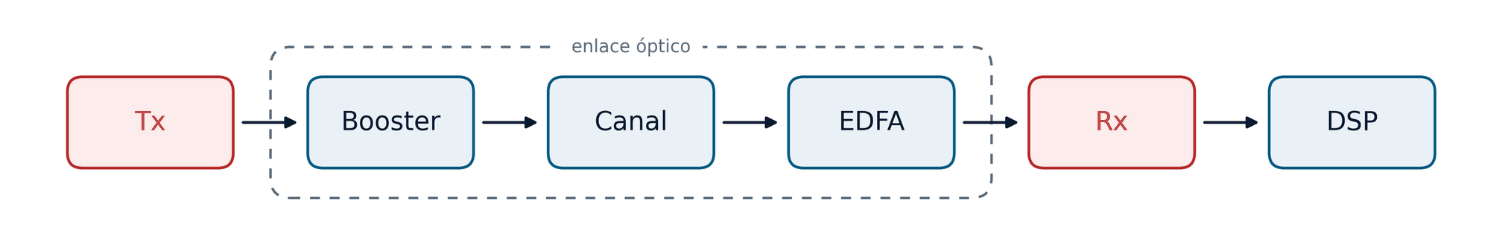
\includegraphics[width=0.95\linewidth]{CadenaOpticaBloques}
  \caption[Cadena completa de simulaci\'on]{%
    Cadena completa de simulaci\'on. En rojo, el transmisor y el receptor, que
    son los bloques que describe este cap\'itulo. Dentro del recuadro
    punteado, el enlace \'optico desarrollado en el \cref{cap:canal}. El DSP
    se trata en el \cref{cap:dsp}.}
  \label{fig:cadena-bloques}
\end{figure}

La \cref{tab:parametros} muestra los par\'ametros principales del transmisor y
del receptor. La elecci\'on de estos par\'ametros se hizo en base a valores de
dispositivos comerciales est\'andar y a los disponibles en el laboratorio, lo
que permite comparar la simulaci\'on con la medici\'on sobre la misma base en
el \cref{cap:experimental}.

\begin{table}[htbp]
\centering

\begin{tabular}{llc}
\toprule
\textbf{Par\'ametro} & \textbf{S\'imbolo} & \textbf{Valor} \\
\midrule
Tasa de s\'imbolo            & $\Rs$              & \SI{32}{\giga\baud} \\
Muestras por s\'imbolo       & SpS                & 16 (sim.) / 2 (DSP) \\
Polarizaciones               & $N_{\mathrm{pol}}$ & 2 \\
Roll-off del RRC             & $\beta$            & 0,2 \\
Longitud de onda             & $\lambda$          & \SI{1550}{\nano\metre} \\
Ancho de l\'inea por l\'aser & $\dnu$             & \SI{100}{\kilo\hertz} \\
Ancho de banda del Front end       & $B_{\mathrm{Rx}}$ & \SI{20}{\giga\hertz} \\
Ancho de banda del ADC       & $B_{\mathrm{ADC}}$ & \SI{33}{\giga\hertz} \\
\bottomrule
\end{tabular}
\caption[Par\'ametros principales de la simulaci\'on]{Par\'ametros principales de la simulaci\'on.}
\label{tab:parametros}
\end{table}

\section{Transmisor}
\label{sec:trx-tx}

\subsection{Generaci\'on de s\'imbolos y conformaci\'on de pulso}
\label{sec:trx-simbolos}

La secuencia de bits a transmitir se mapea en s\'imbolos QPSK con
codificaci\'on Gray, de forma independiente en cada polarizaci\'on. En las
simulaciones de este trabajo se emple\'o una secuencia pseudoaleatoria
PRBS-15, de longitud $2^{15}-1 = \num{32767}$, que es la misma que carga el
generador de patrones del laboratorio.

Los s\'imbolos generados se sobremuestrean a 16 muestras por s\'imbolo para
asegurar una tasa de muestreo de simulaci\'on suficientemente grande como para
representar la se\~nal \'optica sin aliasing. Despu\'es se conforman con un
filtro de ra\'iz de coseno alzado (RRC) de \emph{roll-off} $\beta = 0{,}2$. El
receptor luego incluye un segundo filtro RRC, el filtro adaptado, implementado
tambi\'en en el dominio digital. Entre los dos cumplen el criterio de Nyquist
y anulan la interferencia entre s\'imbolos en el instante de muestreo.

\begin{figure}[H]
  \centering
  \begin{subfigure}[b]{0.48\linewidth}
    \centering
    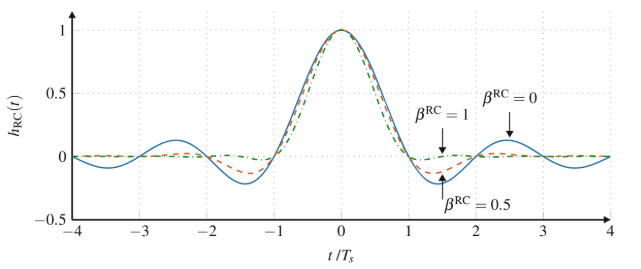
\includegraphics[width=\linewidth]{RRCtiempoLibro}
    \caption{}
  \end{subfigure}
  \hfill
  \begin{subfigure}[b]{0.48\linewidth}
    \centering
    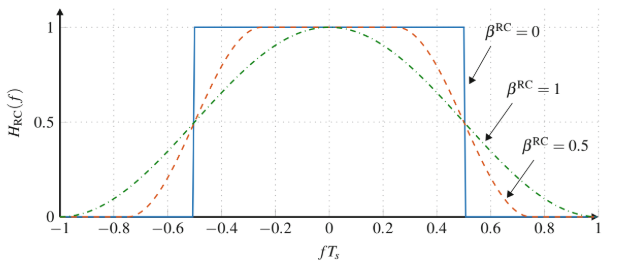
\includegraphics[width=\linewidth]{RRCfrecuenciaLibro}
    \caption{}
  \end{subfigure}
  \caption[Filtro de ra\'iz de coseno elevado]{%
    Filtro de ra\'iz de coseno elevado en tiempo~(a) y en frecuencia~(b) para
    distintos valores de \emph{roll-off}. Adaptado de~\cite{mello2021}.}
  \label{fig:rrc}
\end{figure}

La elecci\'on de $\beta$ presenta una relaci\'on de compromiso, y la
\cref{fig:rrc} lo muestra en los dos dominios. Un \emph{roll-off} chico
angosta el espectro, pero alarga las colas del pulso en el tiempo y lo vuelve
m\'as sensible al error de sincronismo, mientras que un \emph{roll-off} grande
hace lo contrario. A \SI{32}{\giga\baud} con $\beta = 0{,}2$, el ancho de
banda unilateral resulta
\begin{equation}
  B = \frac{\Rs\,(1+\beta)}{2} = \SI{19.2}{\giga\hertz}.
  \label{eq:ancho-senal}
\end{equation}
Con este valor la se\~nal entra justo en los \SI{20}{\giga\hertz} de ancho de
banda del Front end disponible, como se ver\'a en la \cref{sec:trx-rx}. A esto se suma que utilizar valores demasiado peque\~nos de $\beta$ degrada el
detector de error de tiempo de Gardner que se usa en el
\cref{cap:dsp}~\cite[p.~182]{mello2021}. El valor $\beta = 0{,}2$ resulta
entonces un valor razonable teniendo en cuenta el ancho de banda disponible en el receptor y el
margen que necesita la recuperaci\'on de reloj.

\subsection{Modulador DP-IQ}
\label{sec:trx-modulador}

La estructura del modulador se representa en la \cref{fig:modulador}. Se 
la analiza desde adentro hacia afuera, es decir, desde el modulador de fase hasta el modulador de doble polarizaci\'on.

\begin{figure}[H]
  \centering
  \begin{subfigure}[b]{0.47\linewidth}
    \centering
    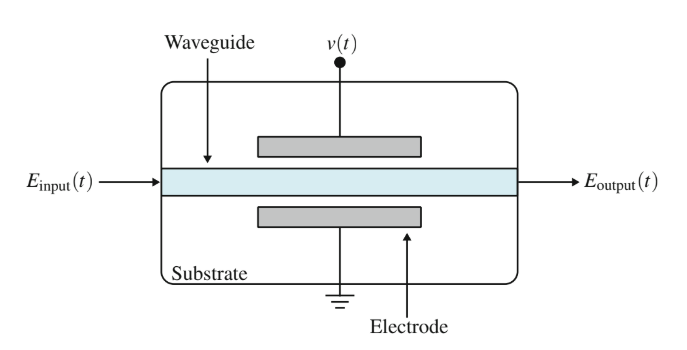
\includegraphics[width=\linewidth]{ModuladorDeFase}
    \caption{Modulador de fase}
  \end{subfigure}
  \hfill
  \begin{subfigure}[b]{0.47\linewidth}
    \centering
    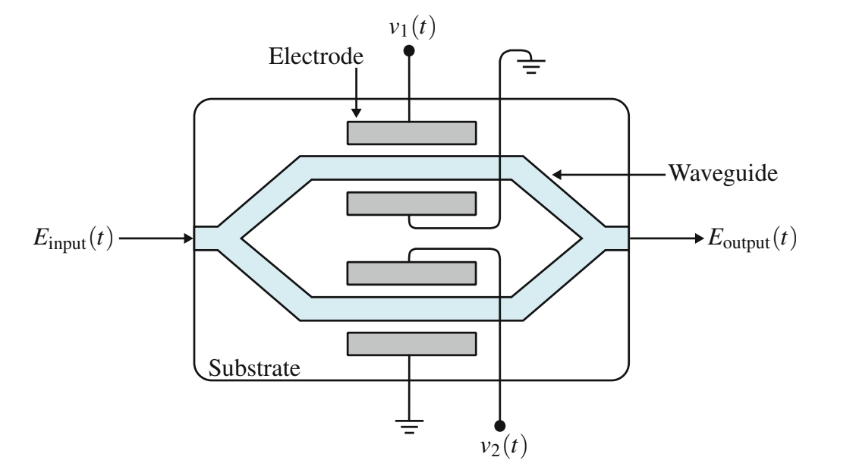
\includegraphics[width=\linewidth]{ModuladorMZM}
    \caption{Mach-Zehnder}
  \end{subfigure}

  \vspace{0.9em}
  \begin{subfigure}[b]{0.52\linewidth}
    \centering
    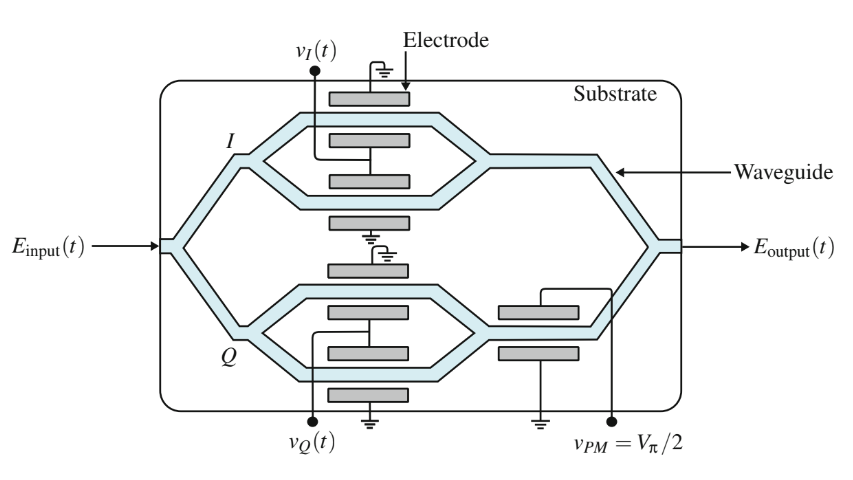
\includegraphics[width=\linewidth]{ModuladorIQ}
    \caption{Modulador IQ}
  \end{subfigure}
  \hfill
  \begin{subfigure}[b]{0.44\linewidth}
    \centering
    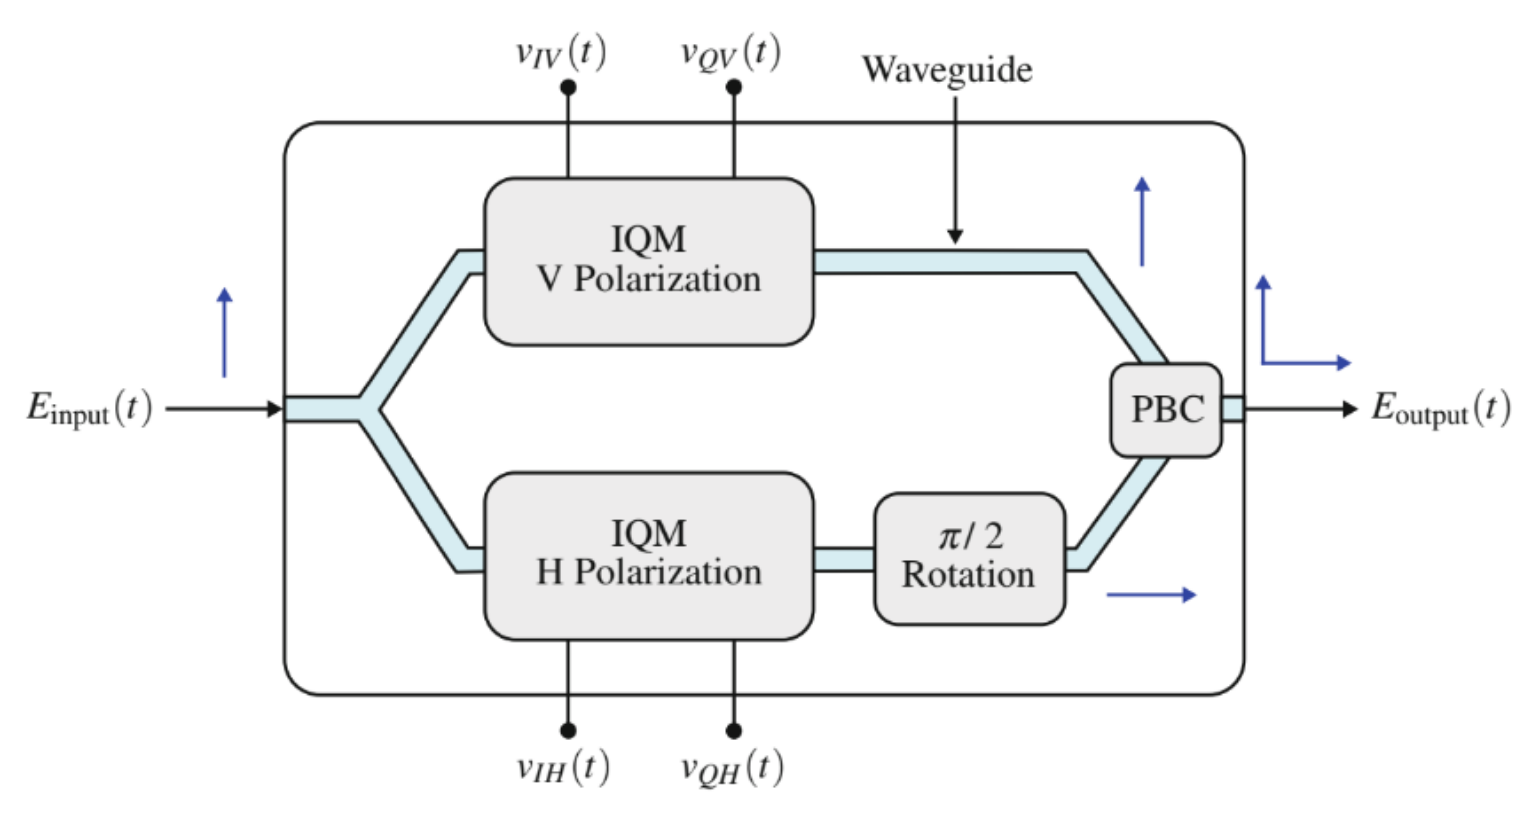
\includegraphics[width=\linewidth]{ModuladorDP}
    \caption{Modulador DP-IQ}
  \end{subfigure}
  \caption[Estructura del modulador DP-IQ]{%
    Estructura anidada del modulador, de adentro hacia afuera. (a)~El
    modulador de fase: un \'unico electrodo sobre una gu\'ia de onda.
    (b)~Dos moduladores de fase en las ramas de un interfer\'ometro forman un
    modulador Mach-Zehnder. (c)~Dos Mach-Zehnder en paralelo, m\'as un
    modulador de fase polarizado en $V_\pi/2$ que introduce el desfasaje de
    $\pi/2$, forman un modulador IQ. (d)~Dos moduladores IQ y un combinador de
    polarizaci\'on (PBC) forman el modulador DP-IQ, con cuatro entradas
    el\'ectricas. Adaptado de~\cite{mello2021}.}
  \label{fig:modulador}
\end{figure}

El componente elemental es el modulador de fase de la \cref{fig:modulador}a.
Este es un electrodo sobre una gu\'ia de onda cuyo \'indice de refracci\'on
depende del campo el\'ectrico aplicado. No cambia la amplitud del campo
entrante, en otras palabras, produce una modulaci\'on de fase proporcional a
la tensi\'on aplicada $v(t)$,
\begin{equation}
  \frac{E_{\mathrm{output}}}{E_{\mathrm{input}}}
     = \exp\!\left(j\,\frac{\pi v}{V_\pi}\right),
  \label{eq:pm}
\end{equation}
donde $E_{\mathrm{input}}$ y $E_{\mathrm{output}}$ son los campos \'opticos a
la entrada y a la salida del dispositivo. La tensi\'on $V_\pi$ es la que
produce un desfasaje de $\pi$ \si{\radian}. En base a esto se construye todo
lo dem\'as.

Poniendo un modulador de fase en cada rama de un interfer\'ometro se obtiene
un modulador Mach-Zehnder, que aparece en la \cref{fig:modulador}b. Si los dos
brazos se manejan con tensiones arbitrarias $v_1$ y $v_2$, la recombinaci\'on
da
\begin{equation}
  \frac{E_{\mathrm{output}}}{E_{\mathrm{input}}}
     = \frac{1}{2}\left[
       \exp\!\left(j\frac{\pi v_1}{V_\pi}\right) +
       \exp\!\left(j\frac{\pi v_2}{V_\pi}\right)\right].
  \label{eq:mzm-general}
\end{equation}

En sistemas de comunicaciones \'opticas coherentes, estos moduladores operan
en lo que se conoce como configuraci\'on push-pull, en la que los dos brazos
se manejan con tensiones id\'enticas y opuestas, $v_1 = -v_2 = v/2$.
Reemplazando en \eqref{eq:mzm-general},
\begin{equation}
  \frac{E_{\mathrm{output}}}{E_{\mathrm{input}}}
     = \frac{1}{2}\left[
       e^{\,j\pi v/2V_\pi} + e^{-j\pi v/2V_\pi}\right]
     = \cos\!\left(\frac{\pi v}{2V_\pi}\right).
  \label{eq:mzm}
\end{equation}

Dos moduladores MZ en paralelo forman un modulador IQ, representado en la
\cref{fig:modulador}c. Cada uno se polariza en el nulo,
$V_{\mathrm{bias}} = -V_\pi$. Una de las dos ramas lleva adem\'as un modulador
de fase fijo en $v_{PM} = V_\pi/2$, que aporta el desfasaje de $\pi/2$ entre
ellas. Llamando $m_I$ y $m_Q$ a las tensiones de modulaci\'on medidas desde el
punto de polarizaci\'on, la salida resulta
\begin{equation}
  \frac{E_{\mathrm{output}}}{E_{\mathrm{input}}}
     = \frac{1}{2}\left[
       \sin\!\left(\frac{\pi m_I}{2V_\pi}\right) +
       j\,\sin\!\left(\frac{\pi m_Q}{2V_\pi}\right)\right],
  \label{eq:iqm}
\end{equation}
donde el seno aparece porque $\cos(\pi(m-V_\pi)/2V_\pi) = \sin(\pi m/2V_\pi)$,
y el factor $1/2$ da cuenta del divisor de entrada y del combinador de salida.
Con \eqref{eq:iqm} se puede obtener la constelaci\'on QPSK a partir de se\~nales
el\'ectricas, $m_I$ y $m_Q$.

Finalmente, el modulador DP-IQ, representado en la \cref{fig:modulador}d, se
construye a partir de dos moduladores IQ y un combinador de polarizaci\'on
(PBC, \emph{polarization beam combiner}). Cada modulador IQ genera una se\~nal
\'optica modulada de manera independiente, a partir de dos se\~nales
el\'ectricas que controlan sus componentes en fase y cuadratura. Las salidas
de ambos moduladores se combinan mediante el PBC en dos polarizaciones
ortogonales. Se obtiene as\'i una se\~nal \'optica con modulaci\'on
independiente en ambas polarizaciones, controlada por las cuatro se\~nales
el\'ectricas $v_{IV}$, $v_{QV}$, $v_{IH}$ y $v_{QH}$.



\subsubsection*{P\'erdidas por modulaci\'on}

Cada Mach-Zehnder se polariza en el nulo de transmisi\'on,
$V_{\mathrm{bias}} = -V_\pi$, que es lo que permite que el campo tome valores
positivos y negativos. La consecuencia es que la se\~nal trabaja sobre la zona
lineal de la ecuaci\'on~\eqref{eq:mzm}, lejos de sus m\'aximos y m\'inimos, lo
que resulta en p\'erdidas de potencia.

\begin{figure}[H]
  \centering
  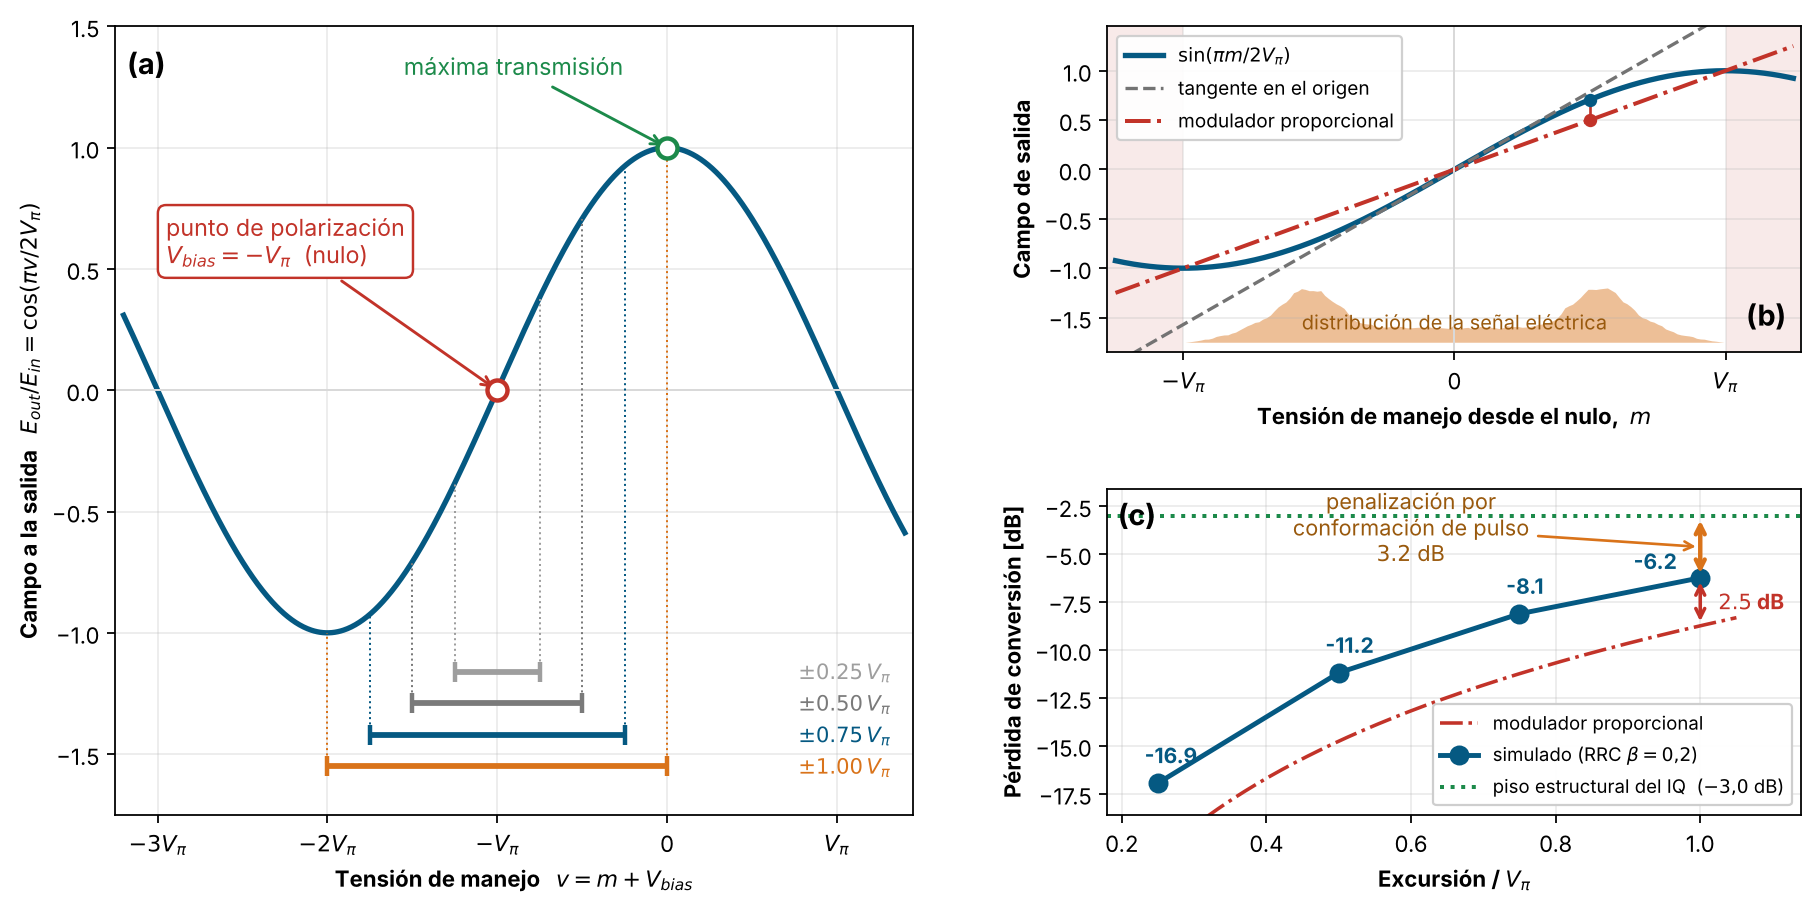
\includegraphics[width=\linewidth]{mzm_punto_polarizacion}
  \caption[Punto de polarizaci\'on y p\'erdida por modulaci\'on del modulador]{%
    Origen de la p\'erdida por modulaci\'on.
    (a)~Polarizado en el nulo, la se\~nal recorre la zona lineal positiva de  $\cos(\pi v/2V_\pi)$. Solo con excursi\'on plena
    $\pm V_\pi$ se llega al m\'aximo del campo.
    (b)~Vista desde el nulo, la transferencia es casi lineal en el centro y se
    comprime cerca de $\pm V_\pi$. Sobre el eje horizontal, la densidad de amplitudes de
    la se\~nal el\'ectrica.
    (c)~P\'erdida contra excursi\'on. La l\'inea punteada es
    el piso de p\'erdida del modulador IQ, \SI{-3.0}{\dB}, que corresponder\'ia
    a se\~nal el\'ectrica binaria. La distancia entre ese piso y el valor simulado
    a excursi\'on plena, \SI{3.2}{\dB}, es la penalidad por conformar el pulso.}
  \label{fig:mzm-bias}
\end{figure}

La \cref{fig:mzm-bias} ilustra el origen de estas p\'erdidas en un modulador
MZ, descomponiendo el efecto en dos contribuciones distintas. La primera es un
piso estructural de \SI{3.01}{\dB}. Si la se\~nal el\'ectrica fuese binaria y
llegara siempre exactamente a $\pm V_\pi$, la ecuaci\'on~\eqref{eq:iqm}
dar\'ia $E_{\mathrm{output}}/E_{\mathrm{input}} = (\pm 1 \pm j)/2$, cuyo
m\'odulo vale $\sqrt{1/2}$. Es decir, un modulador ideal pierde la mitad de
la potencia de entrada. Este es el mejor caso posible de un modulador IQ,
representado por la l\'inea punteada del panel~(c).

La segunda es la penalizaci\'on dependiente de la conformaci\'on del pulso,
que para el \emph{roll-off} adoptado implica \SI{3.2}{\dB} adicionales. Su
origen es el factor de cresta. La se\~nal conformada con RRC pasa la mayor
parte del tiempo lejos de sus picos, con una relaci\'on entre potencia de pico
y potencia media de \SI{5.7}{\dB}. Como la excursi\'on se fija por el
m\'aximo, que no puede superar $V_\pi$, la amplitud media queda muy por debajo
de ese m\'aximo.

La penalizaci\'on, sin embargo, no son \SI{5.7}{\dB} sino \SI{3.2}{\dB}, y la
diferencia la explica la forma de la funci\'on de transferencia. La
\cref{fig:mzm-bias}b compara tres curvas. La primera es la transferencia del
modulador, $\sin(\pi m/2V_\pi)$. La segunda es su tangente en el origen, que
marca el r\'egimen de peque\~na se\~nal. La tercera es la recta que une el
origen con el punto de excursi\'on plena, que es lo que entregar\'ia un
modulador proporcional limitado por el mismo pico. Sobre el eje horizontal se
dibuja adem\'as la densidad de amplitudes de la se\~nal el\'ectrica.

En la \cref{fig:mzm-bias}b, el seno queda por encima de la curva roja en todas las amplitudes
intermedias. A $m = 0{,}5\,V_\pi$ entrega \num{0.71} en lugar de \num{0.50}.
Lo que decide la penalidad, de todos modos, no es un punto aislado sino la
potencia media de salida sobre toda la distribuci\'on de amplitudes.
Promediando sobre la se\~nal conformada, el modulador proporcional entrega
$\langle (m/V_\pi)^2 \rangle = \num{0.266}$ y el modulador real entrega
$\langle \sin^2(\pi m/2V_\pi) \rangle = \num{0.474}$. El cociente entre los
dos son \SI{2.5}{\dB}, que es lo que se recupera de los \SI{5.7}{\dB} del
factor de cresta. La penalidad neta por conformaci\'on resulta entonces de
\SI{3.2}{\dB}.

Sumando las dos contribuciones, la p\'erdida a excursi\'on plena es de
\SI{6.2}{\dB}. Reducir la excursi\'on empeora la p\'erdida r\'apidamente, porque cerca del
nulo la transferencia es casi lineal y la potencia depende entonces del
cuadrado de la se\~nal. Por lo tanto, cada vez que se reduce a la mitad la
excursi\'on se pierden casi \SI{6}{\dB}. A $\pm 0{,}5\,V_\pi$ la p\'erdida es
de \SI{11.2}{\dB} y a $\pm 0{,}25\,V_\pi$ llega a \SI{17.0}{\dB}. Por este
motivo, se decidi\'o como criterio de dise\~no usar un modulador operando a la
m\'axima excursi\'on.

Por \'ultimo, la p\'erdida de \SI{6.2}{\dB} contabiliza \'unicamente la
geometr\'ia de la modulaci\'on, ya que ignora el acoplamiento a fibra, la
propagaci\'on por las gu\'ias de onda, los divisores y el combinador de
polarizaci\'on. Un modulador DP-IQ comercial de niobato de litio para
\SI{32}{\giga\baud} especifica hasta \SI{14}{\dB} de p\'erdida de inserci\'on
total~\cite{fujitsu_ftm7977}. Por este motivo, el balance de potencia del
\cref{cap:enlace} adopta un valor de p\'erdidas de modulaci\'on total de
$L_{\mathrm{DP}} = \SI{14}{\dB}$. El modelo implementado describe bien la
forma de la se\~nal, pero subestima la p\'erdida total del dispositivo.

\section{L\'aser}
\label{sec:trx-laser}

El l\'aser se representa por su campo \'optico complejo, con dos fuentes de
ruido incorporadas al modelo. El ruido de fase se genera como una caminata
aleatoria de incrementos gaussianos con varianza $2\pi\dnu\,T$, que produce el
espectro lorentziano de la \cref{fig:linewidth}. A su vez, el RIN se modela
multiplicando la potencia instant\'anea por un factor aleatorio, de manera que
la fluctuaci\'on de amplitud es siempre una fracci\'on de la potencia.

Escribiendo $P(t) = P_0\,[1 + n(t)]$ con $n$ de media nula, el RIN es la
densidad espectral de esa fluctuaci\'on relativa, y su valor integrado en un
ancho de banda $B$ vale $\sigma_n^2 = \mathrm{RIN}\cdot B$. El campo resulta
\begin{equation}
  E(t) = \sqrt{P_0\,[1+n(t)]}\;e^{\,j\varphi(t)}
       \simeq \sqrt{P_0}\left[1 + \frac{n(t)}{2}\right] e^{\,j\varphi(t)},
  \label{eq:rin-campo}
\end{equation}
donde la aproximaci\'on vale para $|n| \ll 1$ y $\varphi$ es el ruido de fase
descripto arriba. La perturbaci\'on de amplitud tiene entonces potencia
$P_0\,\sigma_n^2/4$, y la relaci\'on se\~nal-ruido que impone el RIN queda
\begin{equation}
  \mathrm{SNR}_{\mathrm{RIN}} = \frac{4}{\mathrm{RIN}\cdot B}.
  \label{eq:snr-rin}
\end{equation}

\begin{figure}[H]
  \centering
  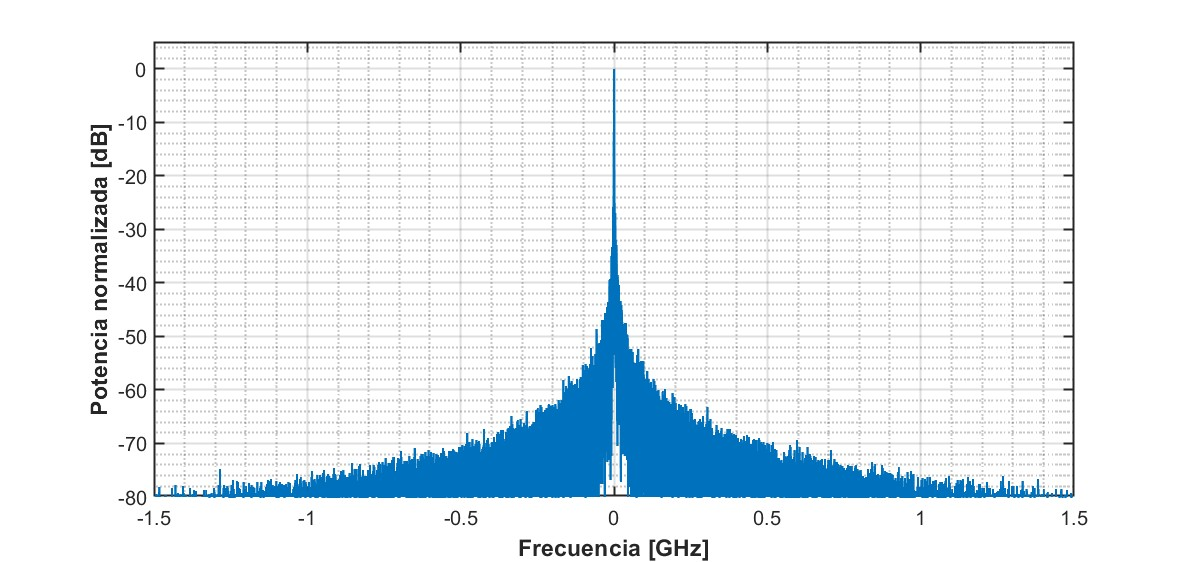
\includegraphics[width=0.72\linewidth]{LineWidth}
  \caption[Espectro del l\'aser simulado]{%
    Espectro de potencia del l\'aser simulado. La forma lorentziana, con las
    colas cayendo como $1/f^2$ alrededor de la portadora, es caracter\'istica del
    ruido de fase modelado como caminata aleatoria.}
  \label{fig:linewidth}
\end{figure}

El l\'aser transmisor y el oscilador local usan el mismo modelo. Sus
par\'ametros se eligieron tomando como referencia un m\'odulo sintonizable
comercial, el PPCL500~\cite{ppcl500}, que cubre toda la banda C con una
potencia de salida de hasta \SI{17}{\dBm}, un ancho de l\'inea 
t\'ipico de \SI{15}{\kilo\hertz} y un RIN de \SI{-140}{\dB\per\hertz}. El RIN
de la simulaci\'on es el correspondiente a la hoja de datos. El ancho de l\'inea, en cambio,
se llev\'o a $\dnu = \SI{100}{\kilo\hertz}$ por l\'aser, un orden de magnitud
por encima del valor real, para exigir al lazo de recuperaci\'on de fase m\'as
de lo que el componente impone.

La tolerancia del receptor a los dos ruidos del l\'aser se analiza en el
\cref{cap:tolerancias}, barriendo cada uno contra una familia de valores de
OSNR.

\section{Front-end coherente y muestreo del receptor}
\label{sec:trx-rx}


El receptor usa una arquitectura de recepci\'on coherente con diversidad de
polarizaci\'on, seg\'un la \cref{fig:receptor}. Un divisor de haz por
polarizaci\'on (PBS) separa las componentes $H$ y $V$ tanto de la se\~nal
recibida como del oscilador local. A su vez, cada par entra a un h\'ibrido de
\SI{90}{\degree} como el descripto en la \cref{sec:coh-deteccion}. Finalmente,
las ocho salidas \'opticas van a parar a cuatro fotodetectores balanceados,
cada uno seguido de su amplificador de transimpedancia y su ADC.

\begin{figure}[H]
  \centering
  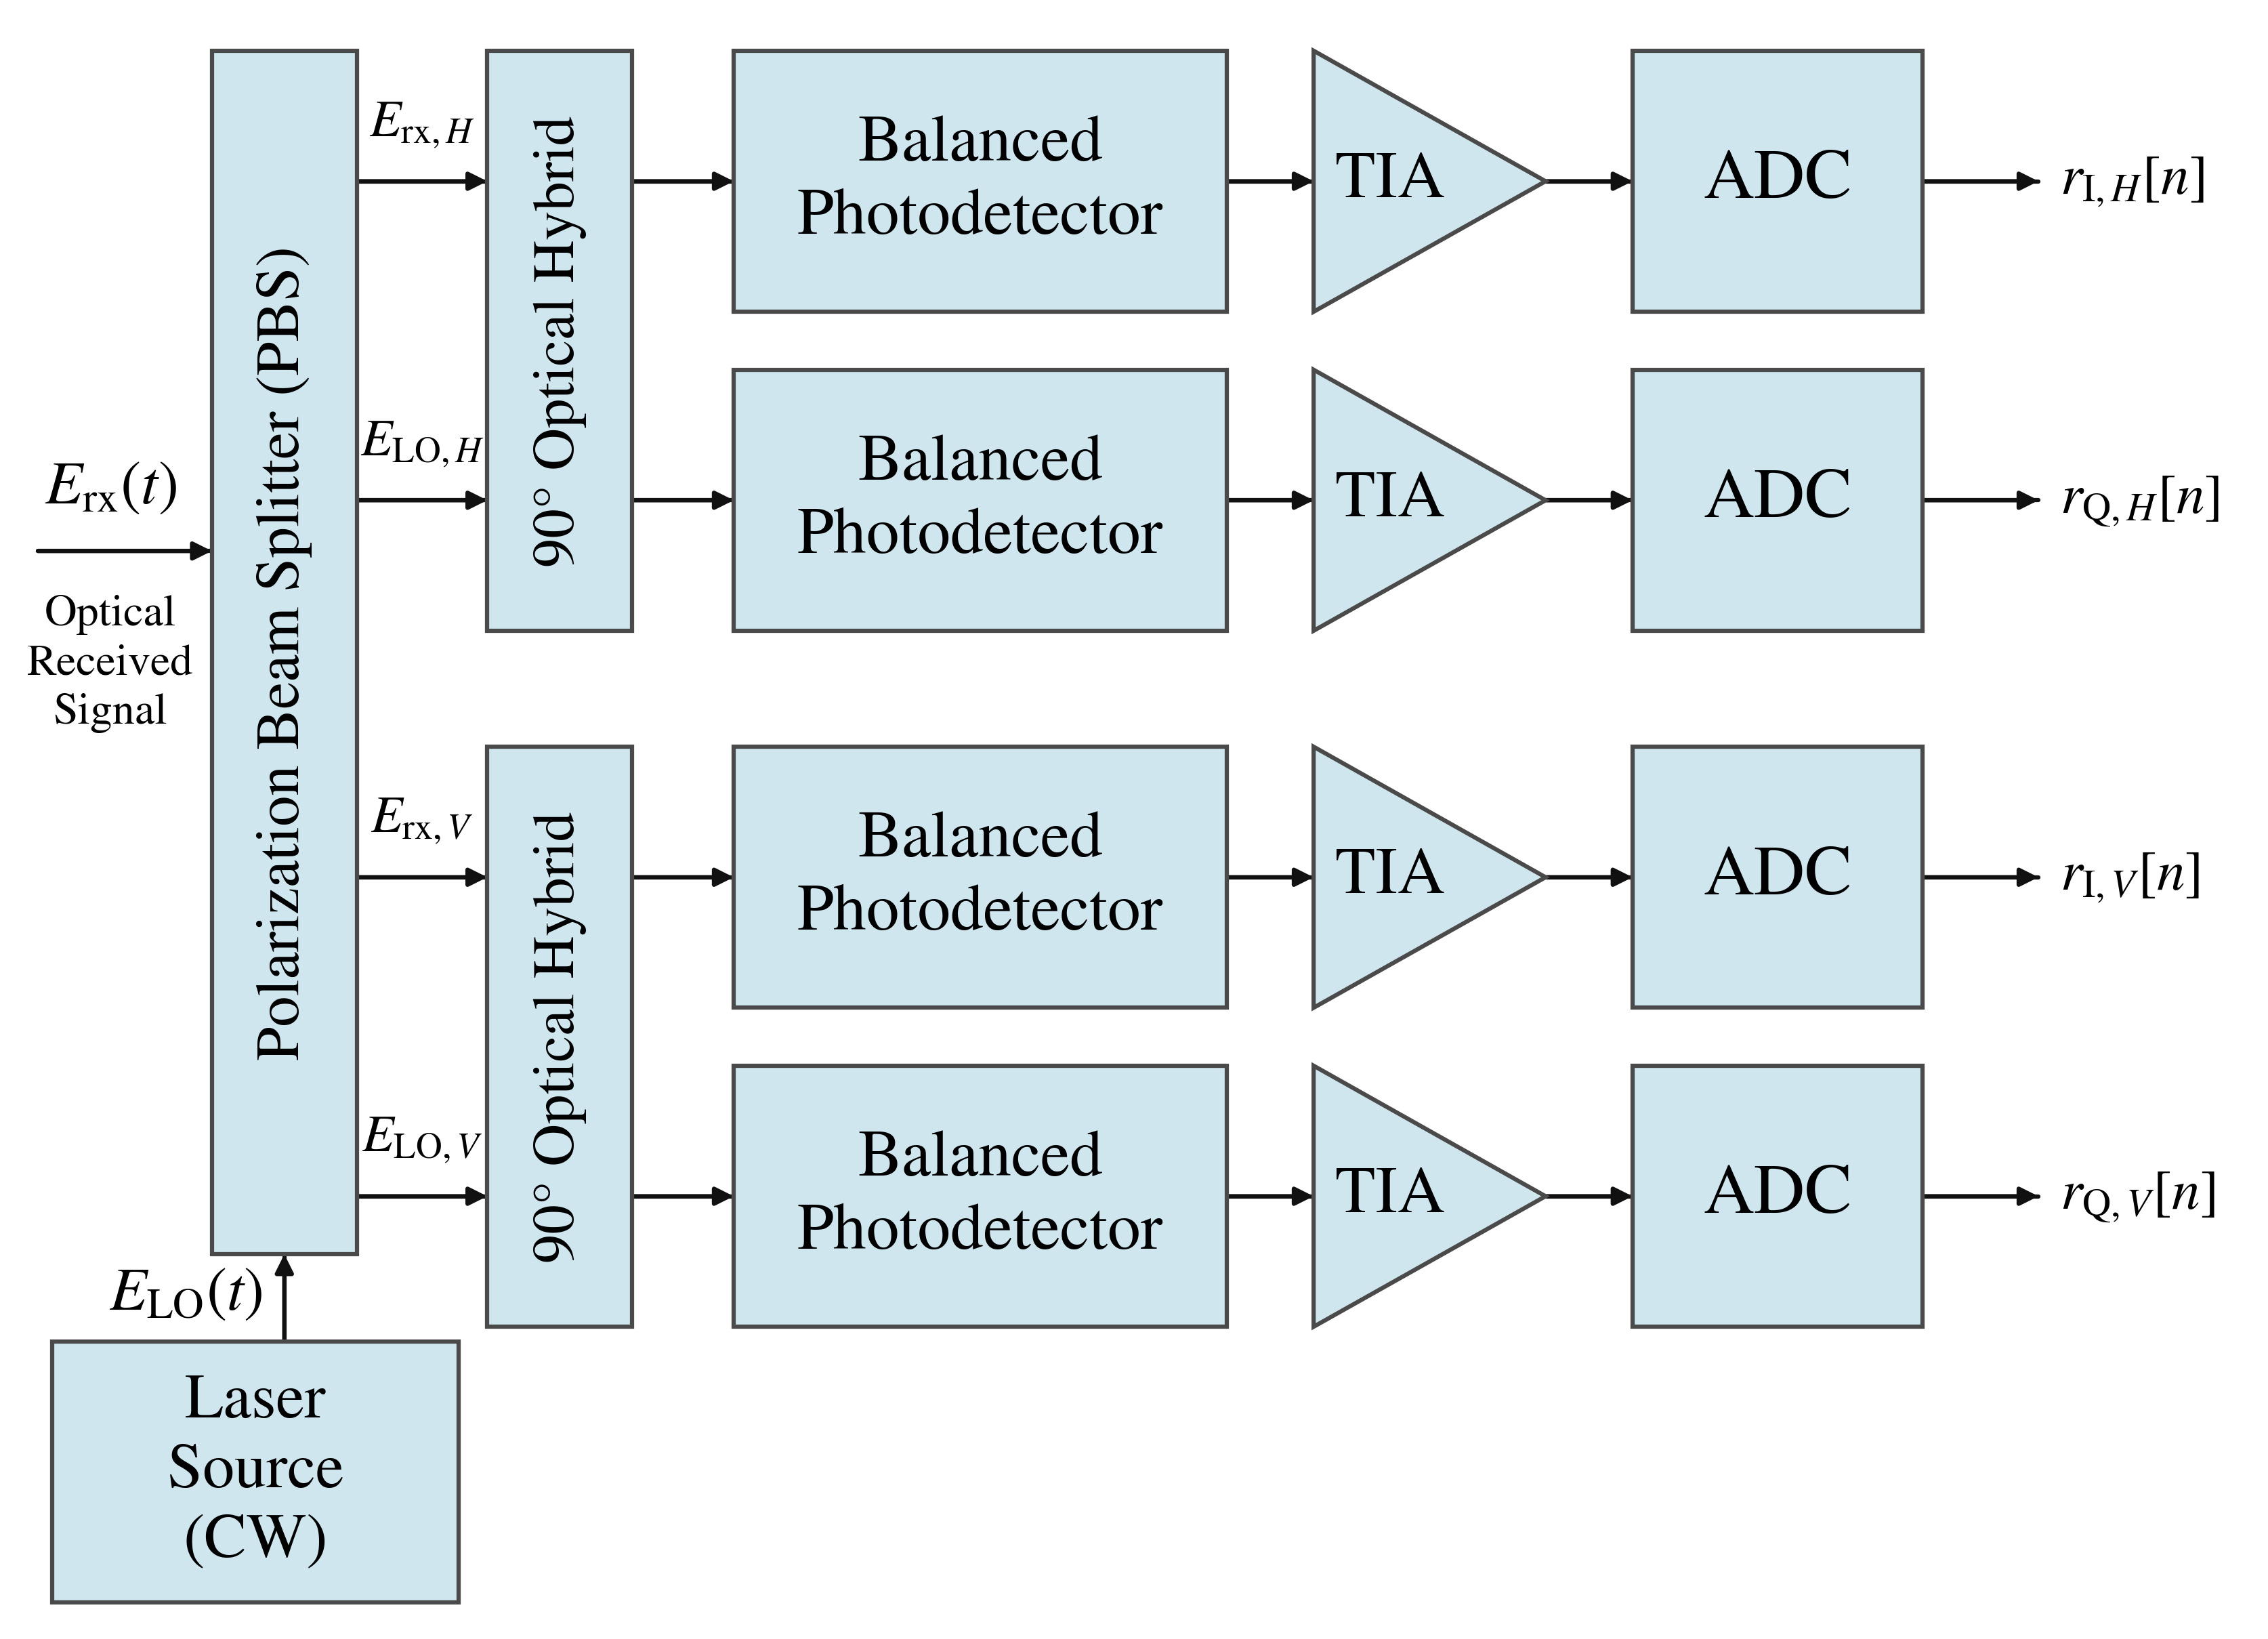
\includegraphics[width=0.72\linewidth]{receptor_esquema}
  \caption[Front end coherente de doble polarizaci\'on]{%
    Front end coherente de doble polarizaci\'on. El mismo oscilador local
    alimenta las dos ramas, de modo que el error de frecuencia y el ruido de
    fase son comunes a las cuatro se\~nales digitalizadas.}
  \label{fig:receptor}
\end{figure}

Como el oscilador local es uno solo para las dos
polarizaciones, el error de frecuencia y el ruido de fase son
comunes a $r_{I,H}$, $r_{Q,H}$, $r_{I,V}$ y $r_{Q,V}$, y eso es lo que permite
estimarlos una \'unica vez sobre las dos polarizaciones en lugar de dos veces
por separado.
\subsection{Respuesta de los fotodiodos, el TIA y el ADC}
\label{sec:trx-anchos}

La respuesta en frecuencia de la cadena de recepci\'on se model\'o con filtros
de Bessel de quinto orden, que aproximan bien la fase lineal de este tipo de
componentes. Se aplican dos, uno por cada limitaci\'on de ancho de banda.

\begin{itemize}\itemsep2pt
  \item El front end \'optico, es decir, los fotodetectores m\'as los
        amplificadores de transimpedancia (TIA), con \SI{20}{\giga\hertz} de
        ancho de banda a \SI{3}{\dB}.
  \item El ADC, con \SI{33}{\giga\hertz} de ancho de banda.
\end{itemize}

Los dos valores se tomaron de las hojas de datos del equipamiento contra el
que despu\'es se contrasta la simulaci\'on en el \cref{cap:experimental}.

\begin{figure}[H]
  \centering
  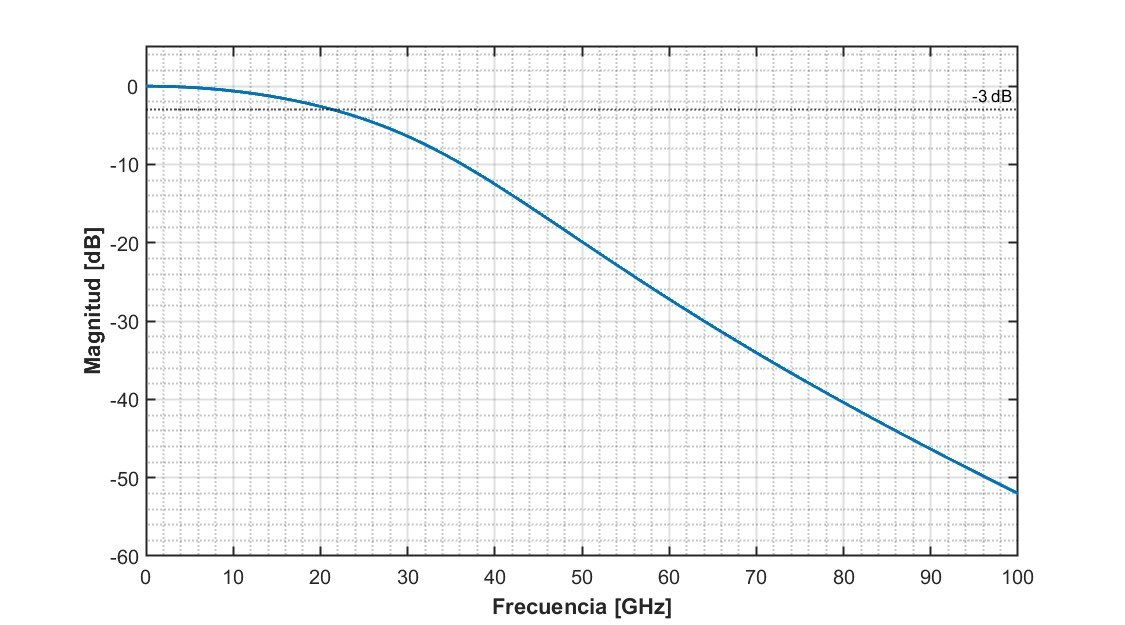
\includegraphics[width=0.70\linewidth]{FiltroTIA_Bessel5toOrden}
  \caption[Respuesta del filtro del TIA]{%
    Respuesta en magnitud del front end, modelado como
    Bessel de quinto orden con el punto de \SI{-3}{\dB} en
    \SI{20}{\giga\hertz}. Los \SI{19.2}{\giga\hertz} que ocupa la se\~nal
    quedan dentro del ancho de banda de \SI{3}{\dB}.}
  \label{fig:filtro-tia}
\end{figure}

La \cref{fig:filtro-tia} muestra la respuesta del front end. Conviene recordar
que la se\~nal ocupa un ancho de banda en banda base de \SI{19.2}{\giga\hertz},
seg\'un la ecuaci\'on~\eqref{eq:ancho-senal}. Este valor cae justo antes del
punto de \SI{-3}{\dB}, de modo que el front end es, de los dos bloques, el que
m\'as recorta el espectro de la se\~nal.

\begin{figure}[H]
  \centering
  \begin{tikzpicture}[
    font=\footnotesize, >={Latex[length=2mm]},
    bl/.style ={draw, rounded corners=3pt, align=center,
                minimum height=3.6em, text width=9.0em, inner sep=3pt},
    cl/.style ={draw=red!40, rounded corners=3pt, fill=red!8, align=center,
                minimum height=3.2em, text width=11.0em, inner sep=3pt},
    fl/.style ={->, thick}
  ]
    \node[bl] (f) {Filtro de Bessel\\[1pt]de quinto orden\\[1pt]
                   $B_{\mathrm{ADC}}=\SI{33}{\giga\hertz}$};
    \node[bl, right=3.0em of f] (s) {Muestreo\\[1pt]$16 \to 2$ muestras\\[1pt]
                   por s\'imbolo};
    \node[cl, below=2.4em of s] (c) {Error de reloj\\[1pt]
                   $t_k = k\,\Ts(1+\delta) + \tau_0$};

    \draw[fl] ($(f.west)-(3.0em,0)$)
      node[left, align=right, font=\scriptsize] {16 muestras\\ por s\'imbolo}
      -- (f.west);
    \draw[fl] (f) -- (s);
    \draw[fl] (c) -- (s);
    \draw[fl] (s.east) -- ++(3.0em,0)
      node[right, align=left, font=\scriptsize] {2 muestras\\ por s\'imbolo};
  \end{tikzpicture}
  \caption[Modelo del ADC]{%
    Modelo del ADC. El filtro de Bessel reproduce la respuesta anal\'ogica de
    la etapa de entrada del conversor. El muestreo posterior lleva la se\~nal a las dos
    muestras por s\'imbolo con las que trabaja el DSP, con
    los instantes afectados por el error de frecuencia de muestreo $\delta$ y
    por el desfasaje inicial $\tau_0$.}
  \label{fig:adc}
\end{figure}

El ADC se representa mediante un modelo simplificado de dos etapas, como
muestra la \cref{fig:adc}. La primera reproduce la respuesta en frecuencia de
la etapa anal\'ogica de entrada del conversor, mediante el filtro pasabajos
de Bessel de quinto orden con ancho de banda de \SI{3}{\dB} de
\SI{33}{\giga\hertz}. La segunda modela el proceso de muestreo, con una
reducci\'on de la tasa de la simulaci\'on de \num{16} a \num{2} muestras por
s\'imbolo, que es la tasa a la que opera el receptor digital. Sobre esta
segunda etapa act\'ua el error de reloj, de modo que los instantes de muestreo
resultan $t_k = k\,\Ts(1+\delta) + \tau_0$, con $\delta$ el error de
frecuencia de muestreo de la \cref{sec:canal-doppler} y $\tau_0$ el desfasaje
inicial.

En cuanto a la conversi\'on de amplitud, se considera un ADC ideal de
resoluci\'on infinita. No se incorpora cuantizaci\'on y las muestras se
mantienen en formato de punto flotante.


\subsection{Elecci\'on de la tasa de muestreo}
\label{sec:trx-nyquist}

El ancho de banda anal\'ogico de un ADC suele quedar por debajo de la mitad de
su frecuencia de muestreo, de modo que la propia etapa de entrada act\'ua como
filtro anti-aliasing. En este caso, el ancho de banda es fijo e igual a \SI{33}{\giga\hertz},
mientras que la frecuencia de muestreo depende de la tasa de s\'imbolo,
$f_s = \mathrm{SpS}\cdot\Rs$. Como este trabajo opera a distintas tasas, la
frecuencia de muestreo cambia con ellas y hace falta verificar que en ning\'un
caso aparezca solapamiento. Lo que decide esa condici\'on es el ancho de banda
de la se\~nal $B$ y no el del conversor.

Se decidi\'o utilizar una tasa de dos muestras por s\'imbolo. Muestrear replica el
espectro cada $f_s$, de modo que la condici\'on de no solapamiento entre
r\'eplicas es $f_s \geq 2B$, es decir
\begin{equation}
  \mathrm{SpS} \geq 1 + \beta = 1{,}2 .
  \label{eq:sps-min}
\end{equation}

\begin{figure}[H]
  \centering
  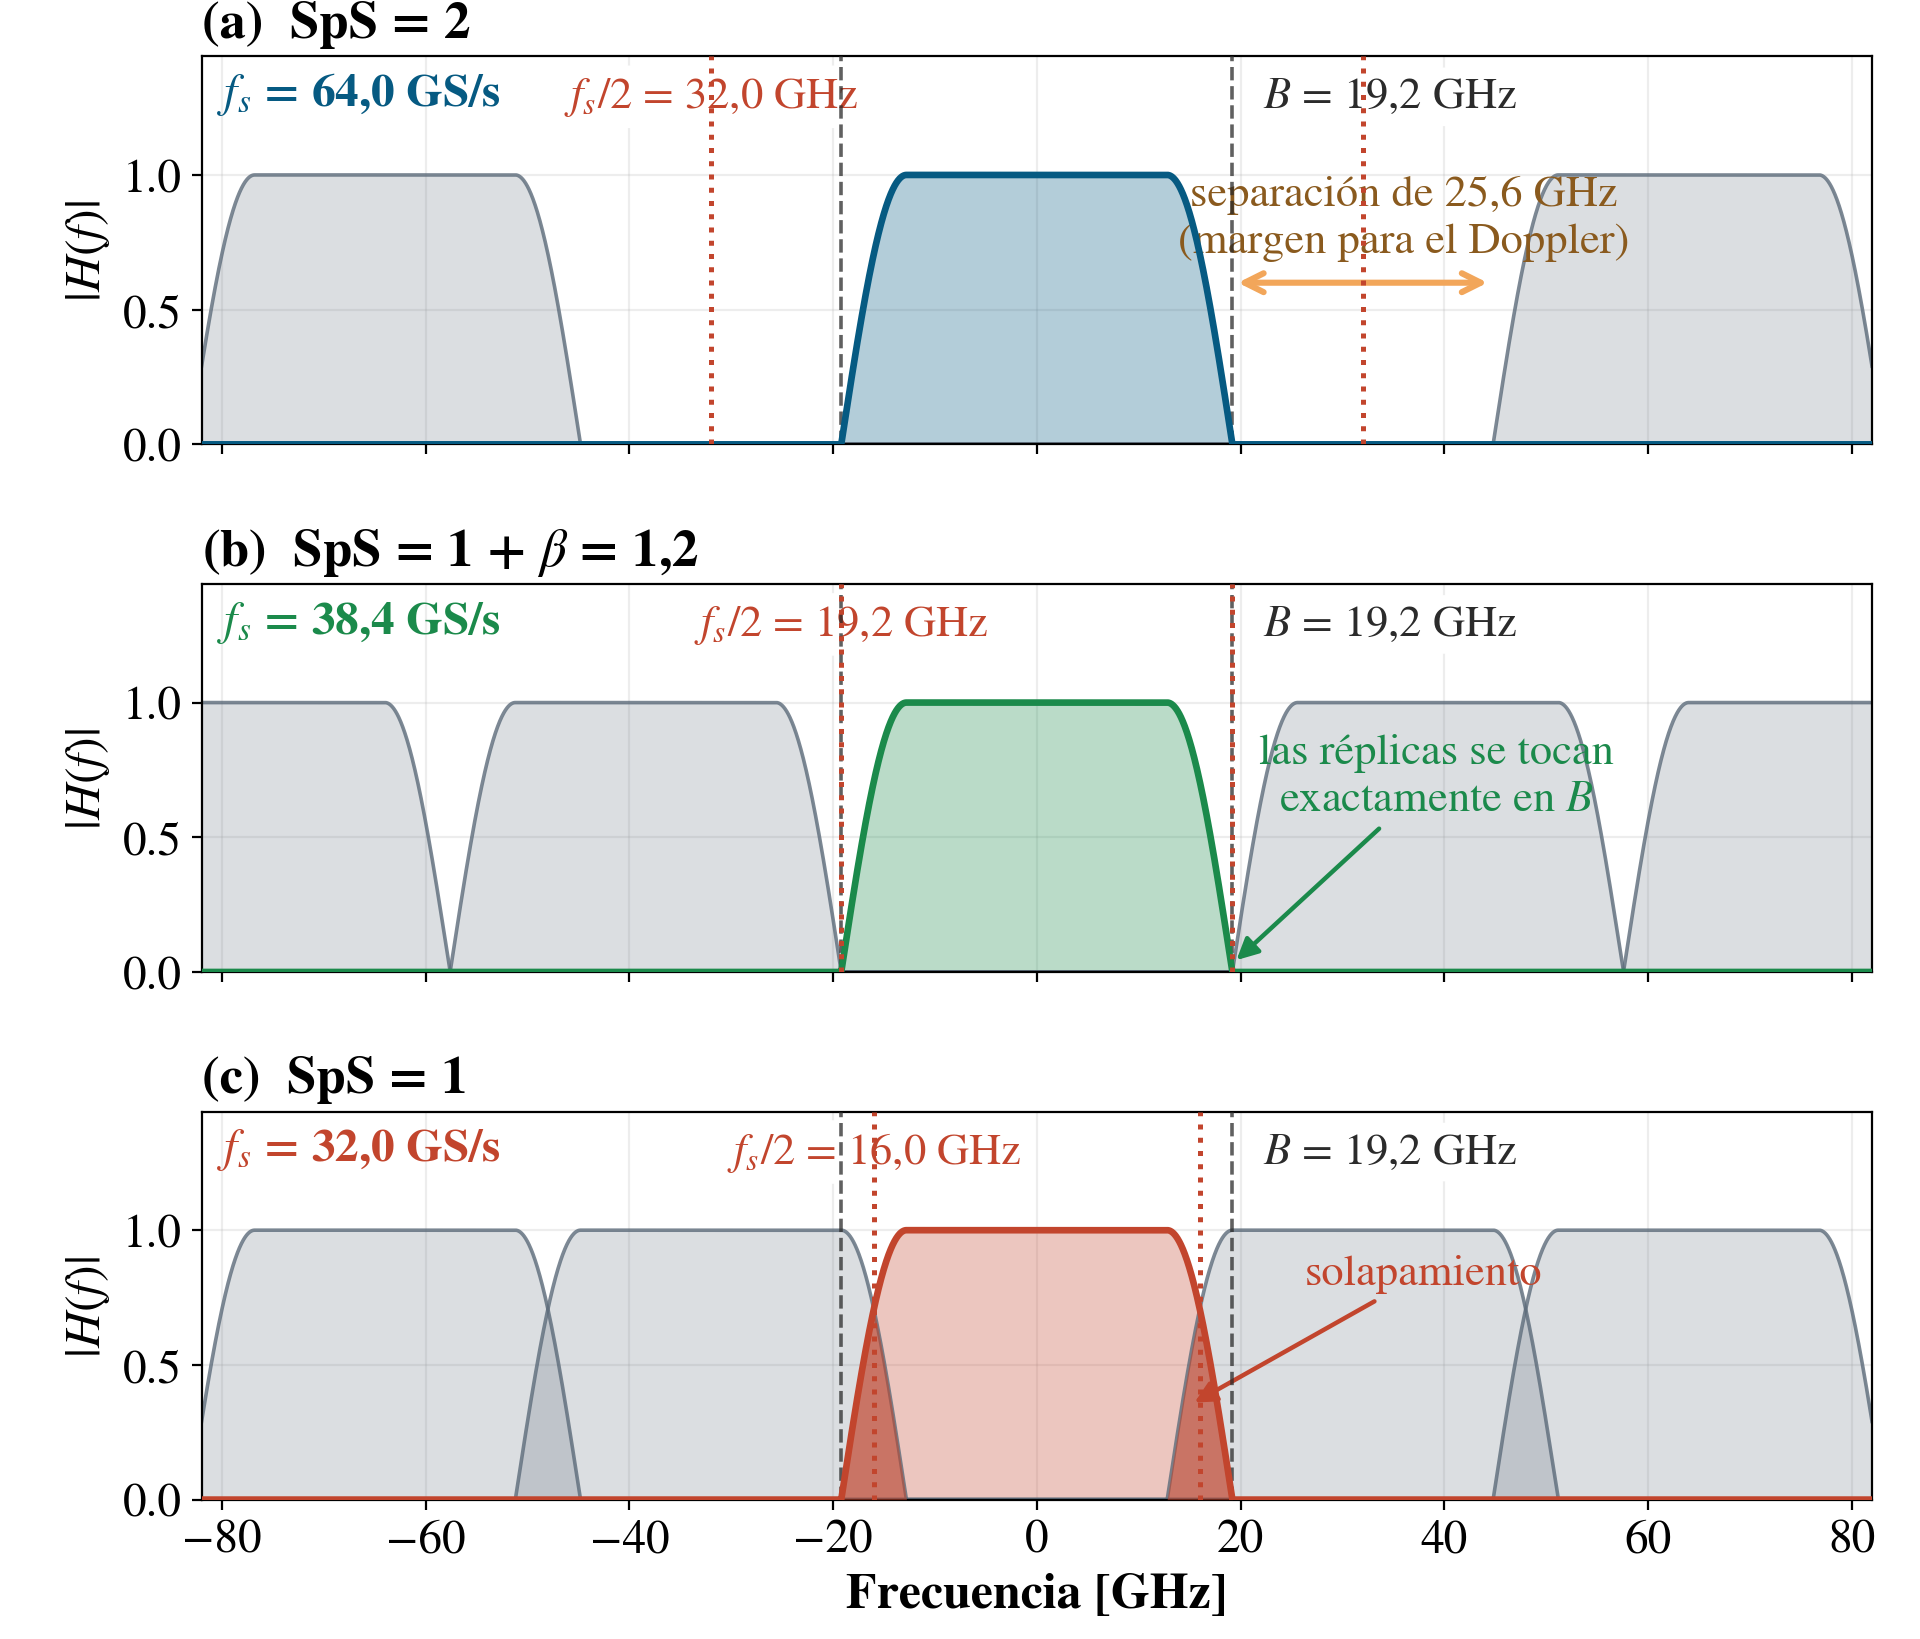
\includegraphics[width=0.88\linewidth]{nyquist_sps}
  \caption[Elecci\'on de la tasa de muestreo]{%
    Espectro muestreado para tres tasas. Con $\mathrm{SpS} = 2$ queda una
    separaci\'on de \SI{25.6}{\giga\hertz} entre la se\~nal y su r\'eplica. Con
    el m\'inimo te\'orico $\mathrm{SpS} = 1{,}2$ las r\'eplicas se tocan
    exactamente en $B$, y con $\mathrm{SpS} = 1$ se superponen y hay aliasing
    irreversible.}
  \label{fig:nyquist}
\end{figure}

La \cref{fig:nyquist} compara las tres situaciones. El m\'inimo te\'orico,
$\mathrm{SpS} = 1{,}2$, deja las r\'eplicas toc\'andose exactamente en $B$, de
modo que cumple Nyquist pero sin ning\'un margen. Con $\mathrm{SpS} = 2$, en
cambio, $f_s = \SI{64}{\giga\hertz}$ y queda una separaci\'on de
\SI{25.6}{\giga\hertz} entre la se\~nal y su r\'eplica.

Este margen es el que absorbe el desplazamiento Doppler. La se\~nal llega
centrada en $\Df$ y ocupa $[\Df - B,\ \Df + B]$, de manera que para que no se
pliegue al muestrear tiene que entrar por completo en la banda,
$\pm f_s/2$. La condici\'on resulta
\begin{equation}
  \abs{\Df} \;\leq\; \frac{f_s}{2} - B
            \;=\; \frac{\Rs\left[\mathrm{SpS} - (1+\beta)\right]}{2},
  \label{eq:doppler-alias}
\end{equation}
que con dos muestras por s\'imbolo se reduce a $\Rs(1-\beta)/2 =
\SI{12.8}{\giga\hertz}$. El requisito de captura del enlace es de
\SI{6.0}{\giga\hertz}, as\'i que el muestreo no es un problema. El verdadero limitante es el recuperador de frecuencia del DSP, cuyo
rango de captura se mide en el \cref{cap:tolerancias}.


\section{Desbalances considerados}
\label{sec:trx-noideal}

Sobre la cadena ideal se inyectan cuatro deterioros que no provienen del canal
sino del equipamiento, resumidos en la \cref{tab:noideal}.

\begin{table}[htbp]
\centering

\begin{tabular}{llc}
\toprule
\textbf{Deterioro} & \textbf{Origen} & \textbf{Valor} \\
\midrule
Desbalance IQ    & h\'ibrido de \SI{90}{\degree}     & \SI{10}{\degree} \\
Skew I/Q         & largo el\'ectrico de los carriles & \SIrange{-1.0}{1.5}{\pico\second} \\
Error de reloj   & Doppler (canal)                   & \SI{25.55}{\ppm}\\
                 & oscilador del Rx (hardware)       & \SI{5}{\ppm} \\
Fase de muestreo & instante de muestreo del ADC      & $0{,}25\,\Ts$\\
\bottomrule
\end{tabular}
\caption[No idealidades inyectadas y su origen f\'isico]{No idealidades inyectadas y su origen f\'isico. El error de reloj
suma dos contribuciones de naturaleza distinta: el Doppler del canal y la
deriva del oscilador local del receptor.}
\label{tab:noideal}
\end{table}

El desbalance IQ es la desviaci\'on de la cuadratura del h\'ibrido, por la cual
las dos salidas no son completamente ortogonales. Un receptor
coherente presenta t\'ipicamente entre \SIrange{1}{5}{\degree}. Se adopt\'o \SI{10}{\degree} para la validaci\'on del DSP.

El skew surge debido a la diferencia entre los caminos el\'ectricos que recorren las ramas I y Q de cada polarizaci\'on. Esta diferencia se acumula en todo el trayecto, desde el híbrido hasta los cables que entran al ADC. A \SI{32}{\giga\baud} un símbolo dura \SI{31.25}{\pico\second}, de modo que \SI{1.5}{\pico\second} son \num{0.048} tiempos de símbolo.

El error de reloj tiene dos or\'igenes distintos. Uno es el Doppler de reloj de la
ecuaci\'on~\eqref{eq:dop-sfo}, \SI{25.55}{\ppm}, que es una propiedad del
canal. Y el otro hace referencia al error de frecuencia de muestreo del ADC del receptor, unos
\SI{5}{\ppm}, que es una propiedad del equipo. Los dos se manifiestan como el
mismo error de frecuencia de muestreo y se inyectan sumados, aunque su origen
sea distinto. A esto se agrega un offset fijo del instante de muestreo, de
$0{,}25\,\Ts$, que representa la falta de sincronismo entre el reloj del
digitalizador y el del transmisor.

\section{Conclusiones}
\label{sec:trx-conclusiones}


En este cap\'itulo se desarroll\'o un modelo general del transmisor y del
receptor, desde la generaci\'on de s\'imbolos hasta el muestreo con error de
reloj y de fase. Los par\'ametros se eligieron despu\'es, tomando como
referencia los dispositivos del laboratorio, lo que permite contrastar
simulaci\'on y medici\'on en el \cref{cap:experimental}.


El modulador opera a excursi\'on plena,
porque reducirla empeora la p\'erdida de modulaci\'on con rapidez. El roll-off
$\beta = 0{,}2$ mantiene la se\~nal dentro del ancho de banda del front end sin privar al detector
de reloj del exceso de ancho de banda que necesita. Las dos muestras por
s\'imbolo dejan lugar para que el offset Doppler desplace la se\~nal dentro de
la banda digitalizada.

El conversor no cuantiza, de modo
que sus \'unicos efectos sobre la se\~nal son el filtrado y el submuestreo. Y el
modelo del modulador contabiliza solo la geometr\'ia de la modulaci\'on, por
lo que subestima la p\'erdida del dispositivo real. El balance de potencia del
\cref{cap:enlace} adopta en su lugar $L_{\mathrm{DP}} = \SI{14}{\dB}$, tomado
de un componente comercial.

Este modelo se utilizado para el resto del trabajo. Los algoritmos que recuperan la
se\~nal se describen en el \cref{cap:dsp}, el balance de potencia en el
\cref{cap:enlace} y los l\'imites de tolerancia de cada deterioro, incluidos
los dos ruidos del l\'aser, en el \cref{cap:tolerancias}.
% !TeX root = ../main.tex
\chapter{Algoritmos del receptor digital}
\label{cap:dsp}
\section{Introducci\'on}
\label{sec:dsp-intro}

En el \cref{cap:transceptor} se obtuvieron las expresiones de las se\~nales
correspondientes a cada uno de los cuatro conversores que componen el
receptor, los cuales digitalizan las componentes en fase y en cuadratura de
las dos polarizaciones ortogonales. En este cap\'itulo se describen los
algoritmos de procesamiento digital implementados en el receptor, encargados
de compensar las degradaciones que introduce el sistema y de realizar la
decisi\'on de s\'imbolo.

En el marco de este proyecto integrador se hace especial \'enfasis en el
algoritmo de recuperaci\'on de frecuencia, ya que es el que fija el l\'imite
de captura del receptor y, por lo tanto, el que determina si el enlace
LEO--GEO resulta viable con el Doppler del \cref{cap:canal}.

\section{Arquitectura de los bloques}
\label{sec:dsp-arquitectura}

La \cref{fig:dsp-cadena} muestra la cadena de algoritmos implementados, desde
la adquisici\'on de las se\~nales hasta la decisi\'on de s\'imbolo final.

\begin{figure}[H]
  \centering
  \resizebox{\linewidth}{!}{%
  \begin{tikzpicture}[
      font=\footnotesize,
      blk/.style={draw, rounded corners=2pt, minimum height=2.6em,
                  text width=6.8em, align=center, inner sep=2pt},
      rx/.style={blk, fill=blue!8},
      bm/.style={blk, fill=orange!12, dashed},
      >={Latex[length=2mm]}]

    \node[rx] (adc)  {ADC\\\scriptsize 2 muestras/s\'imbolo};
    \node[rx, right=0.9em of adc]  (gsop) {Ortogonalizaci\'on\\\scriptsize GSOP};
    \node[rx, right=0.9em of gsop] (foc)  {Recuperaci\'on de frecuencia\\\scriptsize $(\cdot)^4$};
    \node[rx, right=0.9em of foc]  (mf)   {Filtro adaptado\\\scriptsize RRC};
    \node[rx, right=0.9em of mf]   (clk)  {Recuperaci\'on de reloj};

    \node[bm, below=2.6em of clk]  (sync) {Sincronismo con la PRBS};
    \node[rx, left=0.9em of sync]  (eq)   {Ecualizador MIMO\\\scriptsize DD-LMS};
    \node[rx, left=0.9em of eq]    (pll)  {Recuperaci\'on de fase\\\scriptsize PLL};
    \node[rx, left=0.9em of pll]   (dec)  {Decisi\'on};
    \node[bm, left=0.9em of dec]   (met)  {$\BER$ y $\EVM$};

    \draw[->] (adc) -- (gsop);
    \draw[->] (gsop) -- (foc);
    \draw[->] (foc) -- (mf);
    \draw[->] (mf) -- (clk);
    \draw[->] (clk) -- (sync);
    \draw[->] (sync) -- (eq);
    \draw[->] (eq) -- (pll);
    \draw[->] (pll) -- (dec);
    \draw[->] (dec) -- (met);

    \begin{scope}[on background layer]
      \node[draw=blue!45, rounded corners=3pt, inner sep=5pt,
            fit=(eq) (pll)] (lazo) {};
    \end{scope}
    \node[below=0.2em of lazo, font=\scriptsize, blue!45!black]
      {integrados en un solo bloque};

  \end{tikzpicture}}
  \caption[Cadena de procesamiento digital]{%
    Cadena de DSP en el orden en que se ejecuta. En azul, los bloques que
    formar\'ian parte de un receptor de vuelo. En naranja punteado, los dos bloques que utilizan
    la secuencia transmitida: la sincronizaci\'on
    contra la PRBS conocida y el c\'alculo de m\'etricas. El ecualizador y el
    lazo de fase son un solo bloque de c\'odigo, con dos lazos independientes
    adentro.}
  \label{fig:dsp-cadena}
\end{figure}

La cadena consta de seis bloques, cada uno encargado de una degradaci\'on
distinta. El ortogonalizador corrige el desbalance de cuadratura del front end
del receptor. El estimador de cuarta potencia compensa el corrimiento Doppler
de la portadora. El filtro adaptado rechaza el ruido fuera de banda y limita
la interferencia entre s\'imbolos. La recuperaci\'on de reloj corrige el error
de fase de muestreo. El ecualizador MIMO adaptativo compensa la mezcla de
polarizaciones y la interferencia entre s\'imbolos residual. Por \'ultimo, el
lazo de recuperaci\'on de portadora, alojado dentro del mismo ecualizador,
sigue el ruido de fase de los l\'aseres.

Las secciones siguientes describen cada bloque en ese orden. La
justificaci\'on de por qu\'e se eligi\'o ese orden y no otro se desarrolla en
la \cref{sec:dsp-orden}, una vez descriptos todos los algoritmos.

\section{Ortogonalizaci\'on}
\label{sec:dsp-gsop}

\paragraph{Prop\'osito}
Compensa el desbalance de cuadratura del front end del receptor, que hace que
las componentes en fase y en cuadratura de cada polarizaci\'on no sean
ortogonales entre s\'i. El origen de estas imperfecciones est\'a en el
h\'ibrido \'optico de \ang{90} y en la diferencia de ganancia entre los pares
de fotodetectores balanceados.

\paragraph{Principio de operaci\'on}
Se aplica el procedimiento de Gram--Schmidt sobre el par $(r_I, r_Q)$ de cada
polarizaci\'on, donde $r_I$ y $r_Q$ son las se\~nales digitales asociadas a
las componentes en fase y en cuadratura a la salida del
conversor~\cite[ec.~(4.22)--(4.24)]{mello2021}. Se toma $r_I$ como
referencia, se le resta a $r_Q$ su proyecci\'on sobre $r_I$ y se renormaliza,
\begin{equation}
  r_I^{\mathrm{ort}} = \frac{r_I}{\sqrt{\E{r_I^2}}},
  \qquad
  r_Q^{\mathrm{int}} = r_Q - \frac{\E{r_I r_Q}}{\E{r_I^2}}\, r_I,
  \qquad
  r_Q^{\mathrm{ort}} = \frac{r_Q^{\mathrm{int}}}{\sqrt{\E{(r_Q^{\mathrm{int}})^2}}}.
  \label{eq:gsop}
\end{equation}
El \'angulo de cuadratura que se corrige queda expl\'icito como subproducto,
\begin{equation}
  \phi = \arcsin\!\left(\frac{\E{r_I r_Q}}{\sqrt{\E{r_I^2}\,\E{r_Q^2}}}\right).
  \label{eq:gsop-phi}
\end{equation}

\begin{figure}[H]
  \centering
  \begin{subfigure}[b]{0.36\linewidth}
    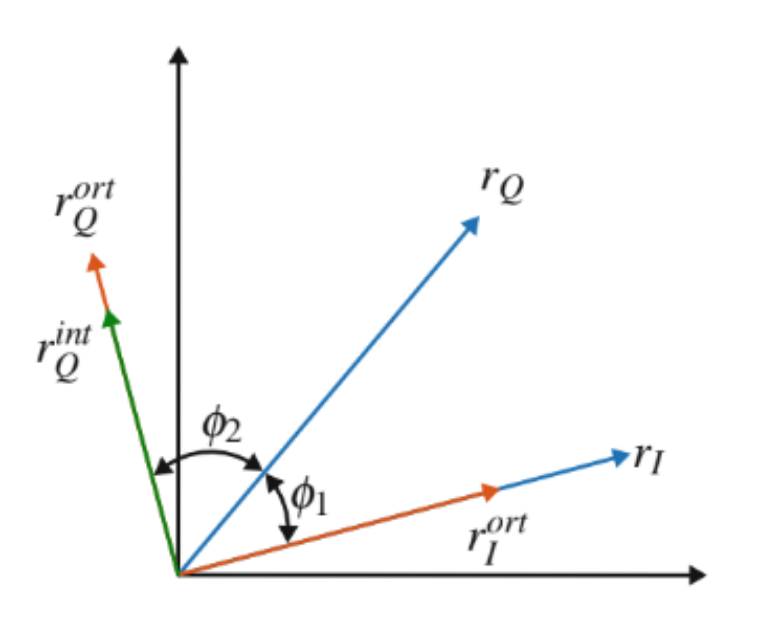
\includegraphics[width=\linewidth]{Ortogonalizador}
    \caption{}
    \label{fig:gsop-vec}
  \end{subfigure}\hfill
  \begin{subfigure}[b]{0.60\linewidth}
    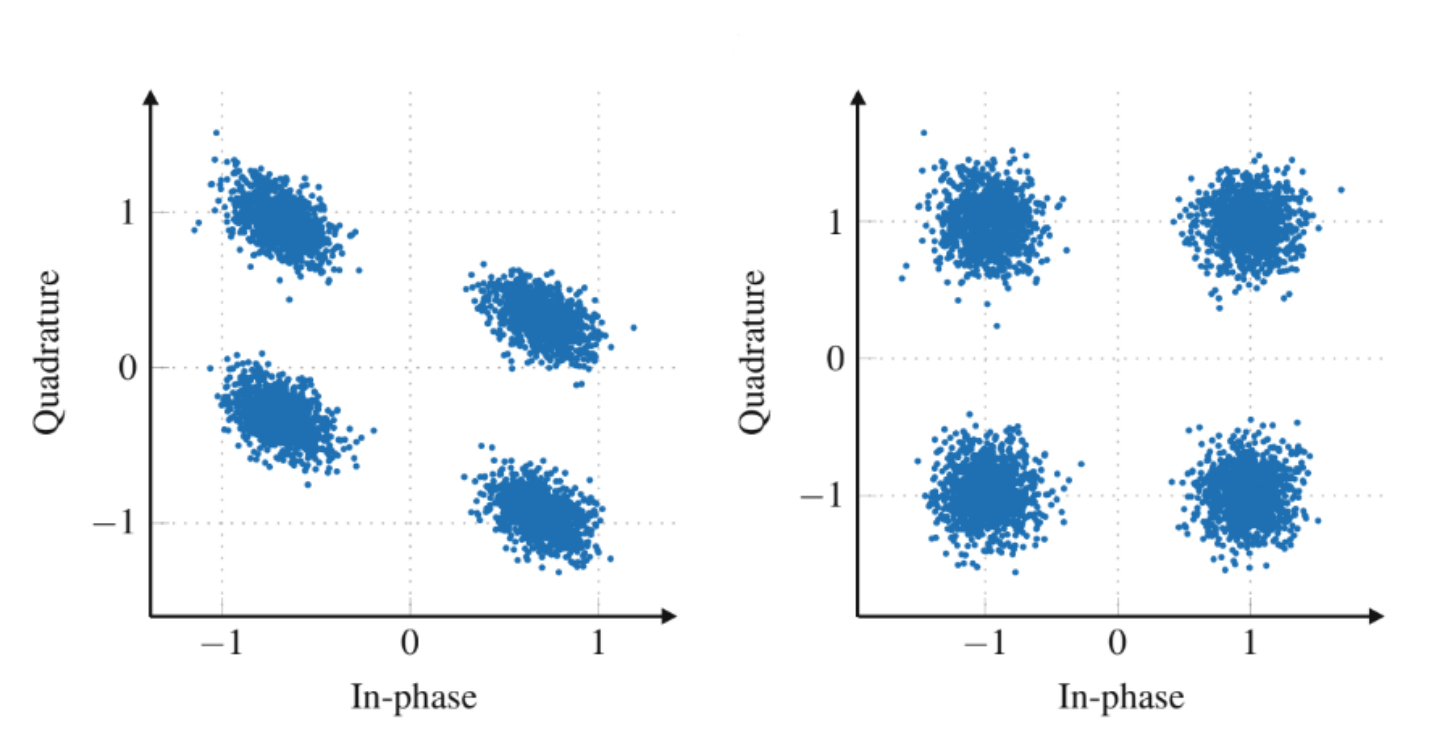
\includegraphics[width=\linewidth]{OrtogonalizadorAntesYDespues}
    \caption{}
    \label{fig:gsop-const}
  \end{subfigure}
  \caption[Ortogonalizaci\'on de Gram--Schmidt]{%
    (a) Construcci\'on: $r_I$ se conserva como referencia y a $r_Q$ se le resta
    su proyecci\'on sobre $r_I$, de modo que $r_Q^{\mathrm{ort}}$ queda
    perpendicular a $r_I^{\mathrm{ort}}$. Los \'angulos $\phi_1$ y $\phi_2$ son
    los que separan a cada carril de su posici\'on ideal. (b) Constelaci\'on
    antes y despu\'es: las nubes inclinadas y el rombo se convierten en nubes circulares.}
  \label{fig:gsop}
\end{figure}

La \cref{fig:gsop} muestra un ejemplo del procedimiento aplicado sobre una
se\~nal QPSK. En el panel~(a) se ve la construcci\'on geom\'etrica, donde los
\'angulos $\phi_1$ y $\phi_2$ miden cu\'anto se aparta cada carril de su
posici\'on ideal. En el panel~(b) se observa el efecto sobre la
constelaci\'on, donde las nubes inclinadas que forman un rombo pasan a ser
circulares y quedan centradas sobre los cuatro puntos ideales, caracter\'istico del ruido aditivo blanco gaussiano.

El procedimiento supone que la se\~nal ideal cumple $\E{s_I s_Q} = 0$, lo cual
vale para QPSK con s\'imbolos independientes. Corrige el \'angulo de
cuadratura y la ganancia relativa, pero no el skew temporal entre las ramas en
fase y en cuadratura. Ese efecto queda a cargo del ecualizador de la
\cref{sec:dsp-ddlms}, que por ser fraccionado en $T/2$ y tener filtros reales
para cada rama puede, en principio, compensarlo.

\paragraph{Verificaci\'on}
El bloque se puso a prueba realizando un barrido param\'etrico de la ganancia
relativa entre las ramas en fase y en cuadratura de las dos polarizaciones,
desde la condici\'on balanceada hasta un cociente de \num{0.30}. El desbalance
se inyect\'o sobre la fotocorriente, que es donde nace una diferencia de
responsividad entre los pares de fotodiodos balanceados.

\begin{figure}[H]
  \centering
  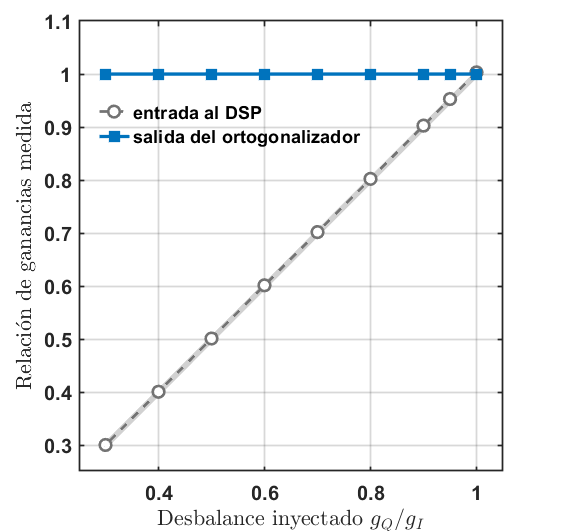
\includegraphics[width=0.6\textwidth]{figuras/DesbalanceGanancias.png}
  \caption[Compensaci\'on del desbalance de ganancia]{%
    Cociente entre la potencia de la rama en cuadratura y la de la rama en
    fase, medido a la entrada del procesamiento y a la salida del
    ortogonalizador, contra el desbalance inyectado.}
  \label{fig:gsop-ganancia}
\end{figure}

La \cref{fig:gsop-ganancia} compara el cociente de potencias a la entrada del
procesamiento y a la salida del ortogonalizador. A la salida vale \num{1.00}
en todo el barrido, y el EVM se mantiene en \SI{31.46}{\percent} en los nueve
puntos. El motivo es que el desbalance se aplica despu\'es de la
fotodetecci\'on y todo lo que sigue hasta el ortogonalizador es lineal, de
modo que el factor llega intacto a la normalizaci\'on y all\'i se cancela. La
medici\'on se hizo con el ruido del preamplificador, que es el dominante del
enlace, y ese ruido lo escalan los fotodetectores igual que a la se\~nal
\'optica, por lo que la relaci\'on se\~nal-ruido no cambia.

Seguidamente se gener\'o un error de desbalance de cuadratura de \ang{10}
junto con el de ganancia, para verificar que el algoritmo es capaz de
estimarlo. El ortogonalizador devuelve \ang{10.26} para todos los valores de
ganancia, lo que verifica la \cref{eq:gsop-phi}.

\section{Recuperaci\'on de frecuencia}
\label{sec:dsp-frec}

Como se describi\'o en la \cref{sec:canal-doppler}, el enlace LEO--GEO impone
un corrimiento Doppler de hasta \SI{4.94}{\giga\hertz} sobre la portadora, al
que se suma la incerteza absoluta de los dos l\'aseres. Por esa raz\'on
resulta necesario estudiar los l\'imites de este bloque.

\paragraph{Prop\'osito}
Compensa la diferencia de frecuencia $\Df$ entre el l\'aser transmisor y el
oscilador local, que en banda base aparece como una rotaci\'on continua de la
constelaci\'on a raz\'on de $2\pi\Df$ radianes por segundo.

\paragraph{Principio de operaci\'on}
Se implement\'o el algoritmo de cuarta potencia, que estima el offset en el
dominio de la frecuencia a partir del espectro de la se\~nal elevada a la
cuarta potencia~\cite[ec.~(6.4)]{mello2021}. La \cref{fig:foc-diagrama} muestra 
la estructura del bloque, donde se ve que
la estimaci\'on se calcula sobre un bloque de muestras y se aplica luego a la
se\~nal completa, sin realimentaci\'on.

Para explicar su funcionamiento, cons\'iderese que la se\~nal compleja
adquirida, en presencia de un offset de frecuencia $\Df$ y en ausencia de
ruido e interferencia entre s\'imbolos, puede escribirse como
\begin{equation}
  y[k] = A\, e^{\,j\left(2\pi\Df\,k/F_s + \theta_0\right)}\,
         e^{\,j\varphi_k}, \qquad
         \varphi_k \in \left\{\tfrac{\pi}{4}, \tfrac{3\pi}{4},
                              \tfrac{5\pi}{4}, \tfrac{7\pi}{4}\right\},
  \label{eq:foc-senal}
\end{equation}
donde $k$ recorre las muestras a la tasa del conversor, $F_s = 2\Rs$, y
$\varphi_k$ es la fase del s\'imbolo QPSK.

Para estimar y posteriormente compensar el valor de $\Df$ se utiliza una propiedad de
QPSK. Las cuatro fases posibles de la modulaci\'on est\'an separadas por
$\pi/2$, as\'i que al elevar a la cuarta potencia
\begin{equation}
  y^4[k] = A^4\, e^{\,j\left(8\pi\Df\,k/F_s + 4\theta_0\right)}\,
           \underbrace{e^{\,j 4\varphi_k}}_{=\,-1\ \forall k},
  \label{eq:foc-cuarta}
\end{equation}
la dependencia con el dato desaparece y lo que queda es una sinusoide pura de
frecuencia $4\Df$. El estimador la ubica computando el valor m\'aximo de la
transformada de Fourier de una secuencia de muestras y divide por cuatro,
\begin{equation}
  \widehat{\Df} = \frac{1}{4}\,
    \arg\max_{f}\ \abs{\mathcal{F}\{y^4[k]\}}.
  \label{eq:foc-estimador}
\end{equation}
La correcci\'on consiste en multiplicar la se\~nal por
$e^{-j2\pi\widehat{\Df}k/F_s}$.

\begin{figure}[H]
  \centering
  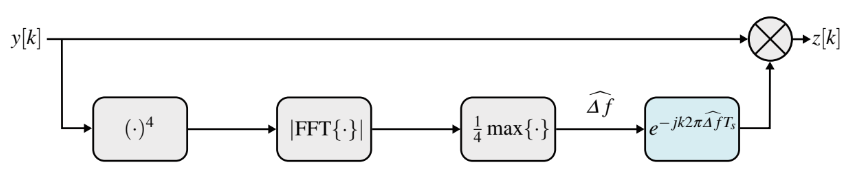
\includegraphics[width=0.86\linewidth]{FRecovery1}
  \caption[Estimador de frecuencia de cuarta potencia]{%
    Estructura del estimador. La rama inferior calcula
    $\widehat{\Df}$ sobre un bloque de muestras y la superior aplica la
    correcci\'on a la se\~nal completa. Es una estimaci\'on de lazo abierto.}
  \label{fig:foc-diagrama}
\end{figure}

\begin{figure}[H]
  \centering
  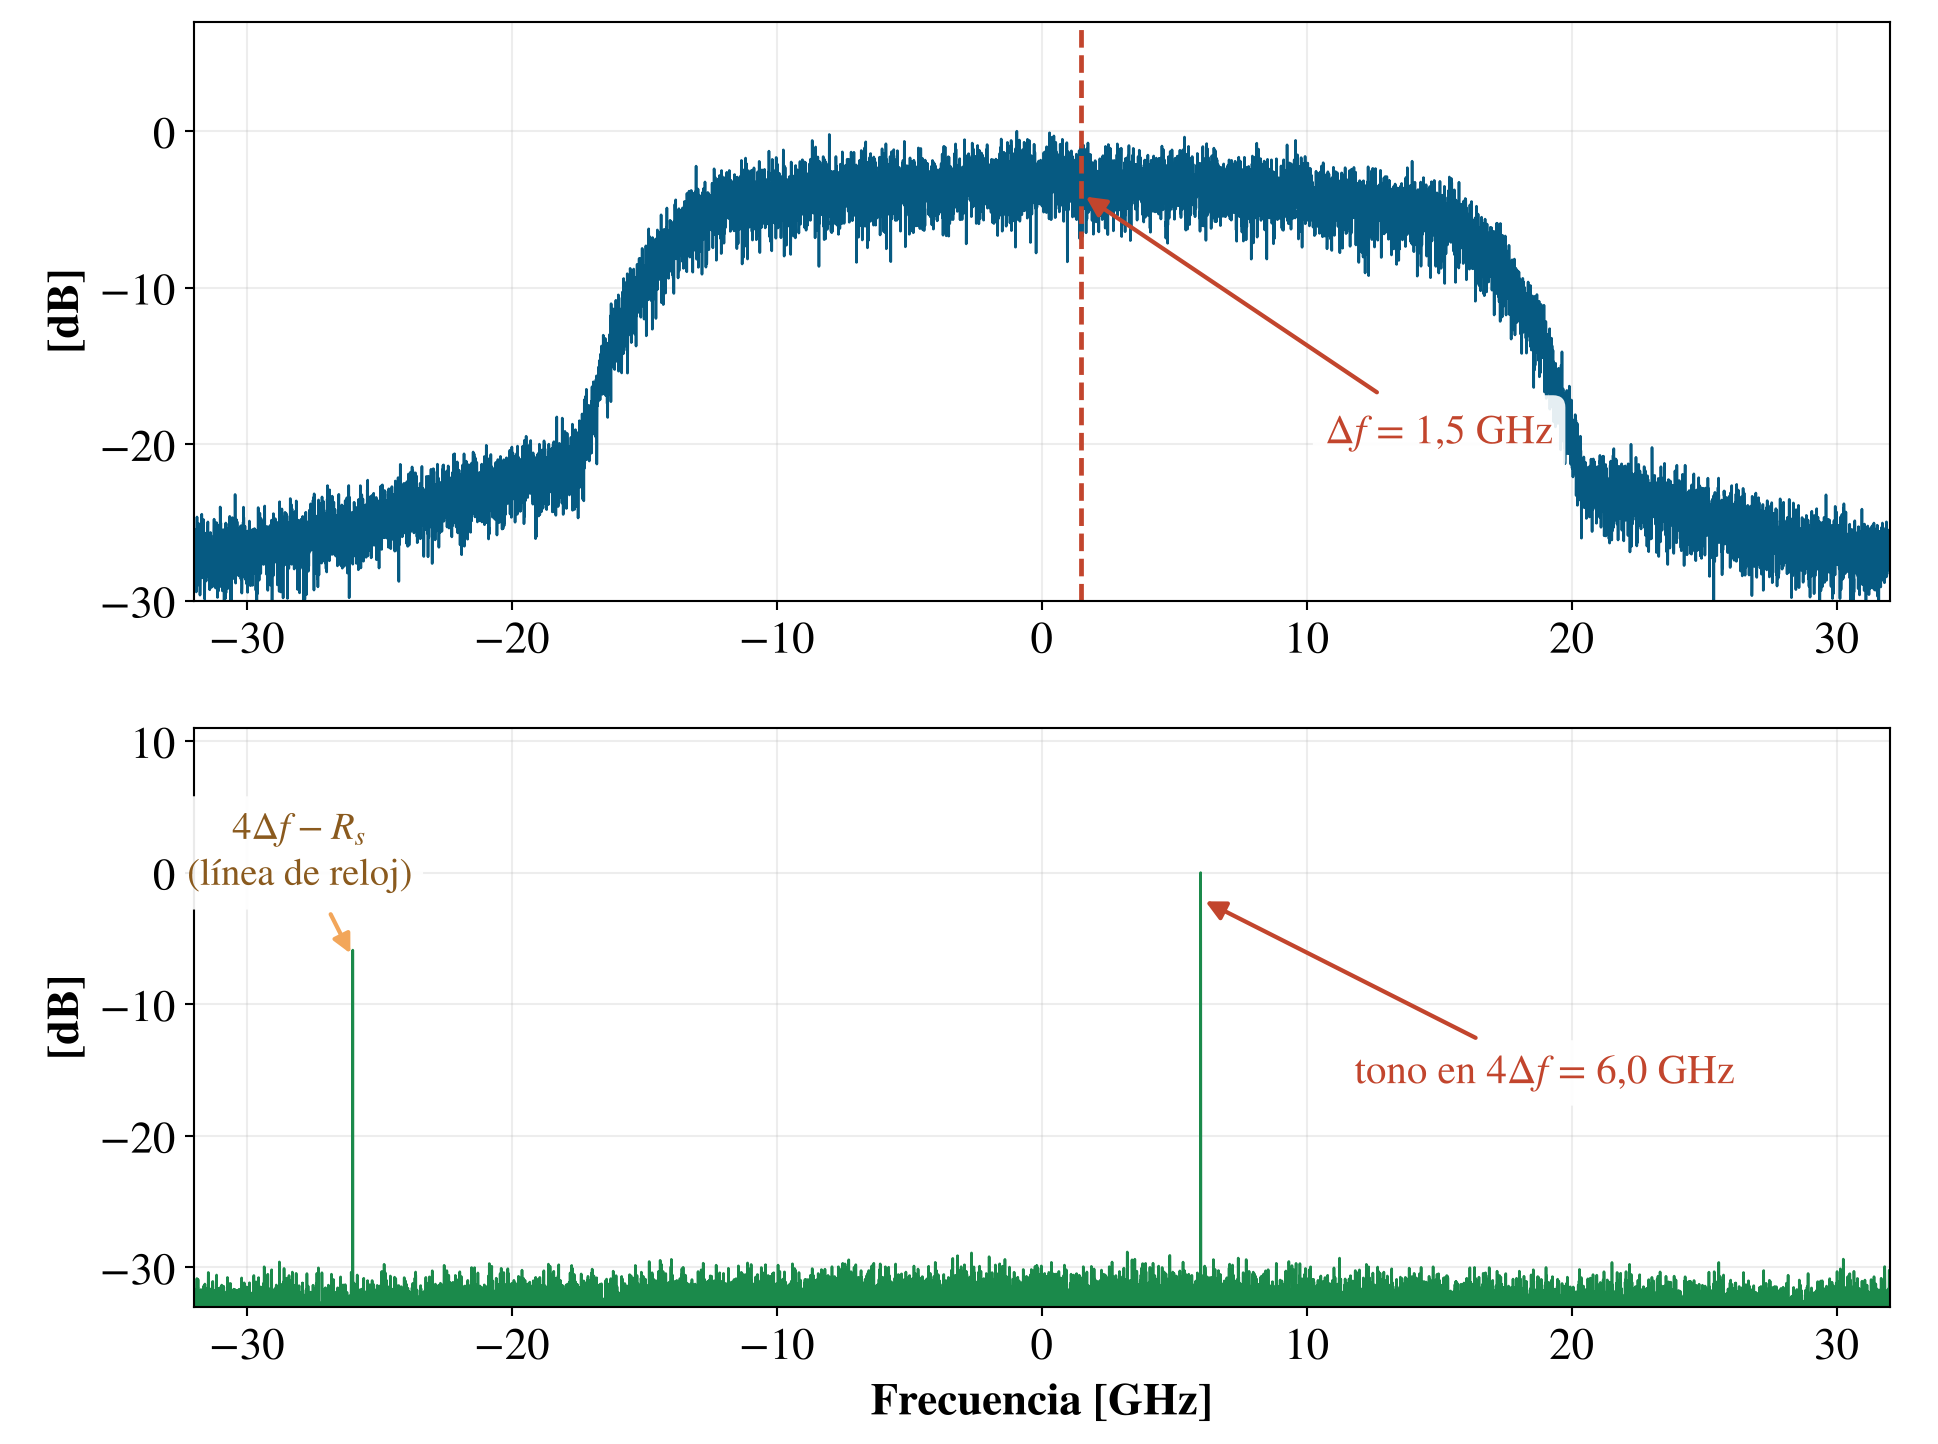
\includegraphics[width=0.9\linewidth]{fourth_power}
  \caption[Espectro antes y despu\'es de elevar a la cuarta potencia]{%
    Simulaci\'on a \SI{32}{\giga\baud} con $\Df = \SI{1.5}{\giga\hertz}$ y
    $\OSNR$ de \SI{16}{\dB}. La imagen superior muestra el espectro de $y[k]$. La inferior muestra c\'omo, elevando a la cuarta potencia, aparece una l\'inea espectral de
    m\'as de \SI{20}{\dB} sobre el piso, exactamente en
    $4\Df = \SI{6}{\giga\hertz}$. La l\'inea de reloj, \SI{6}{\dB} m\'as abajo, est\'a
    en $4\Df - \Rs$.}
  \label{fig:foc-espectro}
\end{figure}

La \cref{fig:foc-espectro} ilustra las
dos etapas del algoritmo sobre el espectro de una simulaci\'on. En el panel
superior, el espectro de $y[k]$ no presenta ninguna l\'inea discreta, porque
la modulaci\'on distribuye la energ\'ia sobre toda la banda. En el inferior, tras
elevar a la cuarta potencia, aparece un tono que sobresale m\'as de
\SI{20}{\dB} del piso y se ubica exactamente en $4\Df$, que es lo que el
estimador busca. Se distingue adem\'as una segunda l\'inea, \SI{6}{\dB} por
debajo y separada $\Rs$ de la principal, cuyo origen y consecuencias se
analizan en la \cref{sec:dsp-frec-limite}.

\subsection{L\'imite de captura}
\label{sec:dsp-frec-limite}

Tres mecanismos distintos pueden limitar el rango de offset que el estimador
resuelve correctamente.

\paragraph{(A) Plegado de Nyquist del tono de cuarta potencia:}
Al elevar a la cuarta potencia, el tono derivado del offset de frecuencia se
encuentra en $4\Df$. Como la se\~nal est\'a muestreada a $F_s = 2\Rs$, la
transformada solo representa frecuencias entre $-F_s/2$ y $+F_s/2$. Si
$4\abs{\Df}$ supera $F_s/2$, el tono cae fuera de ese rango y reaparece
plegado por el borde opuesto, donde el estimador lo toma como v\'alido. De
modo que el m\'aximo offset de frecuencia tolerado para que el estimador
funcione sin ambig\"uedad es
\begin{equation}
  \abs{\Df} < \frac{F_s}{8} = \frac{\Rs}{4} = \SI{8}{\giga\hertz}
  \qquad (\text{a } \Rs = \SI{32}{\giga\baud}).
  \label{eq:limite-nyquist}
\end{equation}

\begin{figure}[H]
  \centering
  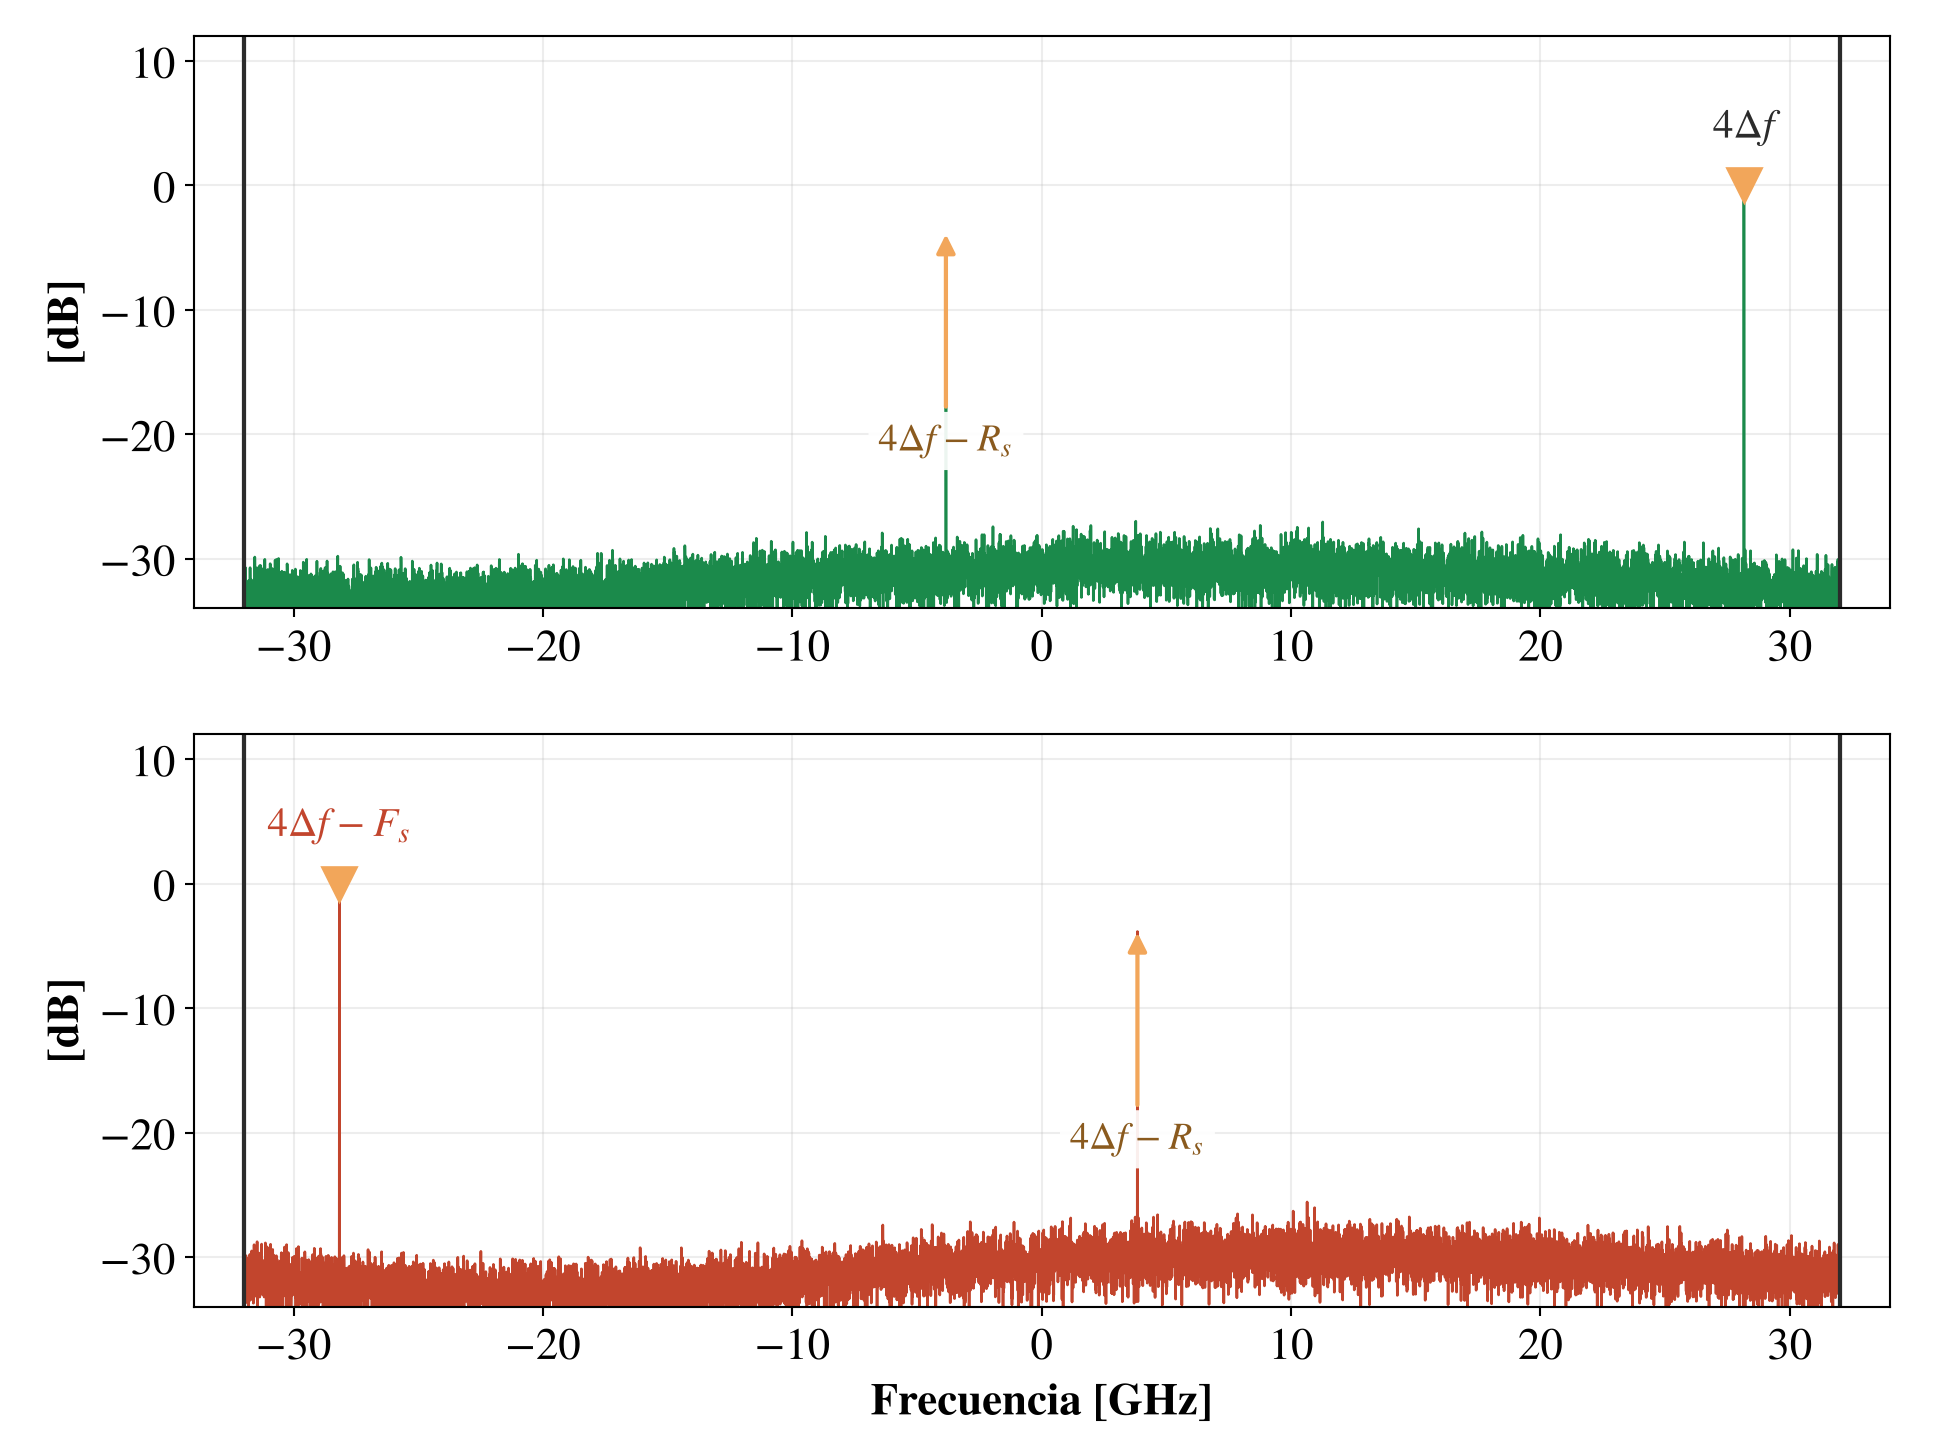
\includegraphics[width=0.9\linewidth]{limite_captura}
  \caption[Techo de captura por plegado de Nyquist]{%
    Espectro de $y^4[k]$ a los dos lados del techo~(A). Arriba, con
    $\Df = 0{,}22\,\Rs$ el tono de cuarta potencia cae dentro de la banda y la
    estimaci\'on es exacta. Abajo, con $\Df = 0{,}28\,\Rs$ el tono deber\'ia
    estar en \SI{35.84}{\giga\hertz}, fuera de $\pm F_s/2$. Sin embargo, reaparece plegado en
    \SI{-28.16}{\giga\hertz} y el estimador devuelve \SI{-7.04}{\giga\hertz} en
    lugar de \SI{8.96}{\giga\hertz}, un salto de $-\Rs/2$. En los dos paneles se
    ve tambi\'en la l\'inea de reloj en $4\Df - \Rs$, que en el panel de abajo ya
    est\'a a \SI{3.7}{\dB} del pico.}
  \label{fig:foc-limite}
\end{figure}

La \cref{fig:foc-limite} muestra un ejemplo de lo que ocurre a los dos lados
del umbral. En el panel superior, con $\Df = 0{,}22\,\Rs$, el tono de
cuarta potencia cae dentro de la banda representable y la estimaci\'on
coincide con el valor inyectado. En el inferior, con $\Df = 0{,}28\,\Rs$, el
tono deber\'ia ubicarse en \SI{35.84}{\giga\hertz}, por encima de $F_s/2$. Se
puede observar c\'omo reaparece en \SI{-28.16}{\giga\hertz}, de donde el
estimador devuelve \SI{-7.04}{\giga\hertz} en lugar de
\SI{8.96}{\giga\hertz}. El salto es de $-\Rs/2$ y ocurre sin degradaci\'on
previa, porque no se trata de una p\'erdida de precisi\'on sino de una
ambig\"uedad del rango representable.

\paragraph{(B) L\'inea de reloj:}
La ciclo\-estacionariedad del pulso conformado genera adem\'as l\'ineas
espectrales en $4\Df \pm k\Rs$. A medida que el offset
crece, el tono principal se acerca al borde de la banda del receptor, donde el
front end de \SI{20}{\giga\hertz} y el conversor de \SI{33}{\giga\hertz} lo
aten\'uan, mientras que la l\'inea ubicada $\Rs$ m\'as abajo queda en una zona
menos atenuada. Si llegara a superar al tono principal, la estimaci\'on
tendr\'ia un salto de  $-\Rs/4$, distinto al que produce el plegado y por lo
tanto reconocible.

El mecanismo se observa en las dos figuras anteriores. Con
$\Df = \SI{1.5}{\giga\hertz}$ la l\'inea de reloj est\'a \SI{6}{\dB} por
debajo del tono principal, y con el offset mayor de la \cref{fig:foc-limite}
esa distancia ya se redujo a \SI{3.7}{\dB}. En ninguna de las condiciones
ensayadas con $\beta = 0{,}2$ lleg\'o a predominar antes de alcanzarse el
l\'imite~(A).

\paragraph{(C) Ancho de banda de adquisici\'on:}
Este l\'imite no es debido al estimador sino al muestreo, y se dedujo en la
\cref{sec:trx-nyquist}. La se\~nal llega centrada en $\Df$ y ocupa
$[\Df - B,\ \Df + B]$, con $B = (1+\beta)\Rs/2$, de manera que para no
plegarse tiene que entrar por completo en la banda del
conversor,
\begin{equation}
  \abs{\Df} \leq \frac{F_s}{2} - B .
  \label{eq:limite-adc}
\end{equation}
Con $F_s = 2\Rs = \SI{64}{\giga\hertz}$ y $B = \SI{19.2}{\giga\hertz}$ el
l\'imite vale \SI{12.8}{\giga\hertz}, holgadamente por encima del techo~(A).


\paragraph{Conclusi\'on}
El mecanismo que predomina en la cadena simulada es el~(A). No se trata de una
degradaci\'on progresiva ni de una cuesti\'on de relaci\'on se\~nal-ruido,
sino del rango de la funci\'on que implementa el estimador, que busca un
m\'aximo sobre un eje de frecuencias acotado a $\pm F_s/2$. Para $\Rs = \SI{32}{\giga\baud}$,
\begin{equation}
  \abs{\widehat{\Df}} \leq \frac{\Rs}{4} = \SI{8}{\giga\hertz}.
  \label{eq:techo-duro}
\end{equation}

El requerimiento del enlace, establecido en el \cref{cap:canal}, es de
\SI{6.0}{\giga\hertz}, de los cuales \SI{4.94}{\giga\hertz} corresponden al
Doppler y \SI{1}{\giga\hertz} a la incerteza combinada de los dos l\'aseres.
Contra el l\'imite de \SI{8}{\giga\hertz} queda un \SI{33}{\percent} de margen.

El rango de captura escala \'unicamente con $\Rs$, de modo que bajar la tasa
de s\'imbolo lo reduce en la misma proporci\'on. El \cref{cap:tolerancias}
verifica estos l\'imites sobre un barrido de offset, y analiza en qu\'e medida
la relaci\'on se\~nal-ruido y el ancho de banda del receptor los modifican.

\section{Filtro adaptado y recuperaci\'on de reloj}
\label{sec:dsp-mf-clock}

\subsection{Filtro adaptado}
\label{sec:dsp-mf}

\paragraph{Prop\'osito}
Maximiza la relaci\'on se\~nal-ruido en el instante de decisi\'on y, junto con
la conformaci\'on de pulso del transmisor, completa el par que en principio
cumple el criterio de Nyquist.

\paragraph{Principio de operaci\'on}
Se trata del mismo RRC del transmisor, con $\beta = 0{,}2$, implementado como filtro
FIR a la tasa del conversor.

\begin{figure}[H]
  \centering
  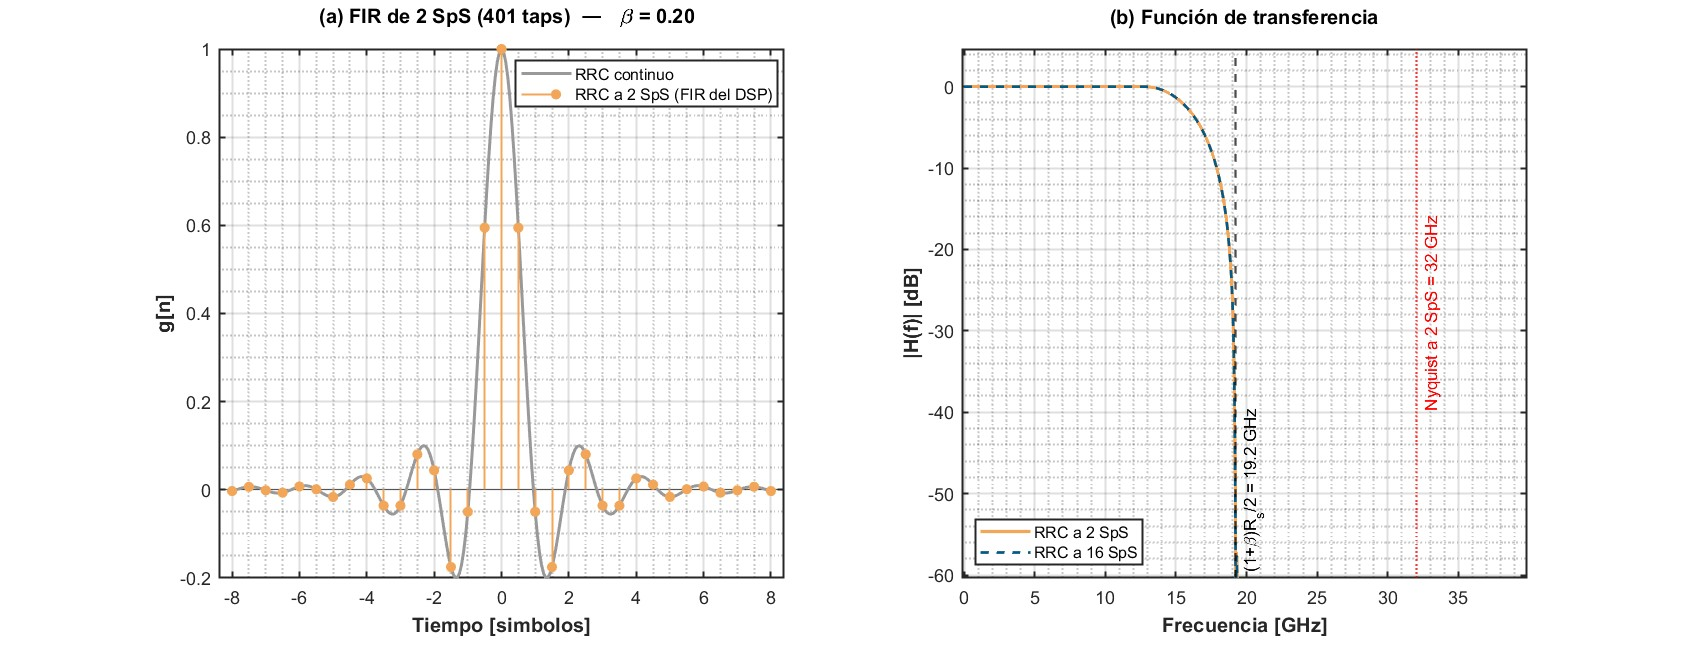
\includegraphics[width=0.95\linewidth]{FiltroFIRdelDSP}
  \caption[Filtro adaptado del receptor]{%
    (a) Respuesta al impulso: los \num{401} coeficientes del FIR caen
    exactamente sobre el RRC continuo. (b) Funci\'on de transferencia: la versi\'on a
    \num{2} muestras por s\'imbolo coincide con la de \num{16} hasta muy por debajo de
    $(1+\beta)\Rs/2 = \SI{19.2}{\giga\hertz}$, y el borde de Nyquist a \num{2}
    muestras por s\'imbolo, que est\'a en \SI{32}{\giga\hertz}, queda holgadamente por encima.}
  \label{fig:fir}
\end{figure}

La \cref{fig:fir} verifica que implementarlo a dos muestras por s\'imbolo no
altera su respuesta en la banda de inter\'es. En el panel~(a) se observa que
los \num{401} coeficientes del FIR caen sobre la respuesta del RRC continuo.
En el panel~(b) se compara la funci\'on de transferencia a dos y a dieciséis
muestras por s\'imbolo, y las dos coinciden hasta bastante m\'as all\'a del
borde de la se\~nal. El borde de Nyquist a dos muestras por s\'imbolo queda en
\SI{32}{\giga\hertz}, holgadamente por encima de los
\SI{19.2}{\giga\hertz} que la se\~nal ocupa.

Cabe resaltar que la cadena completa no cumple el criterio de Nyquist. Entre
los dos filtros RRC se interpone la respuesta del front end de
\SI{20}{\giga\hertz} y la del conversor de \SI{33}{\giga\hertz}, que recortan
el pulso y dejan interferencia entre s\'imbolos residual. Esa es una de las
razones por las que el ecualizador adaptativo de la \cref{sec:dsp-ddlms}
resulta necesario aun sin considerar los deterioros del canal.

\subsection{Lazo de recuperaci\'on de reloj}
\label{sec:dsp-clock}

\paragraph{Prop\'osito}
Por otro lado, la recuperaci\'on de reloj corrige el error de fase de muestreo
que aparece porque el conversor del receptor no est\'a sincronizado con el
reloj del transmisor. A esto se suma el desv\'io de la tasa de s\'imbolo de
\SI{25.55}{\ppm} que introduce el Doppler (\cref{sec:canal-doppler}).

\paragraph{Principio de operaci\'on}
El bloque reconstruye el valor que la se\~nal habr\'ia tenido en el instante
de muestreo correcto, interpolando entre las muestras disponibles. El instante
lo fija un lazo cerrado.

\begin{figure}[H]
  \centering
  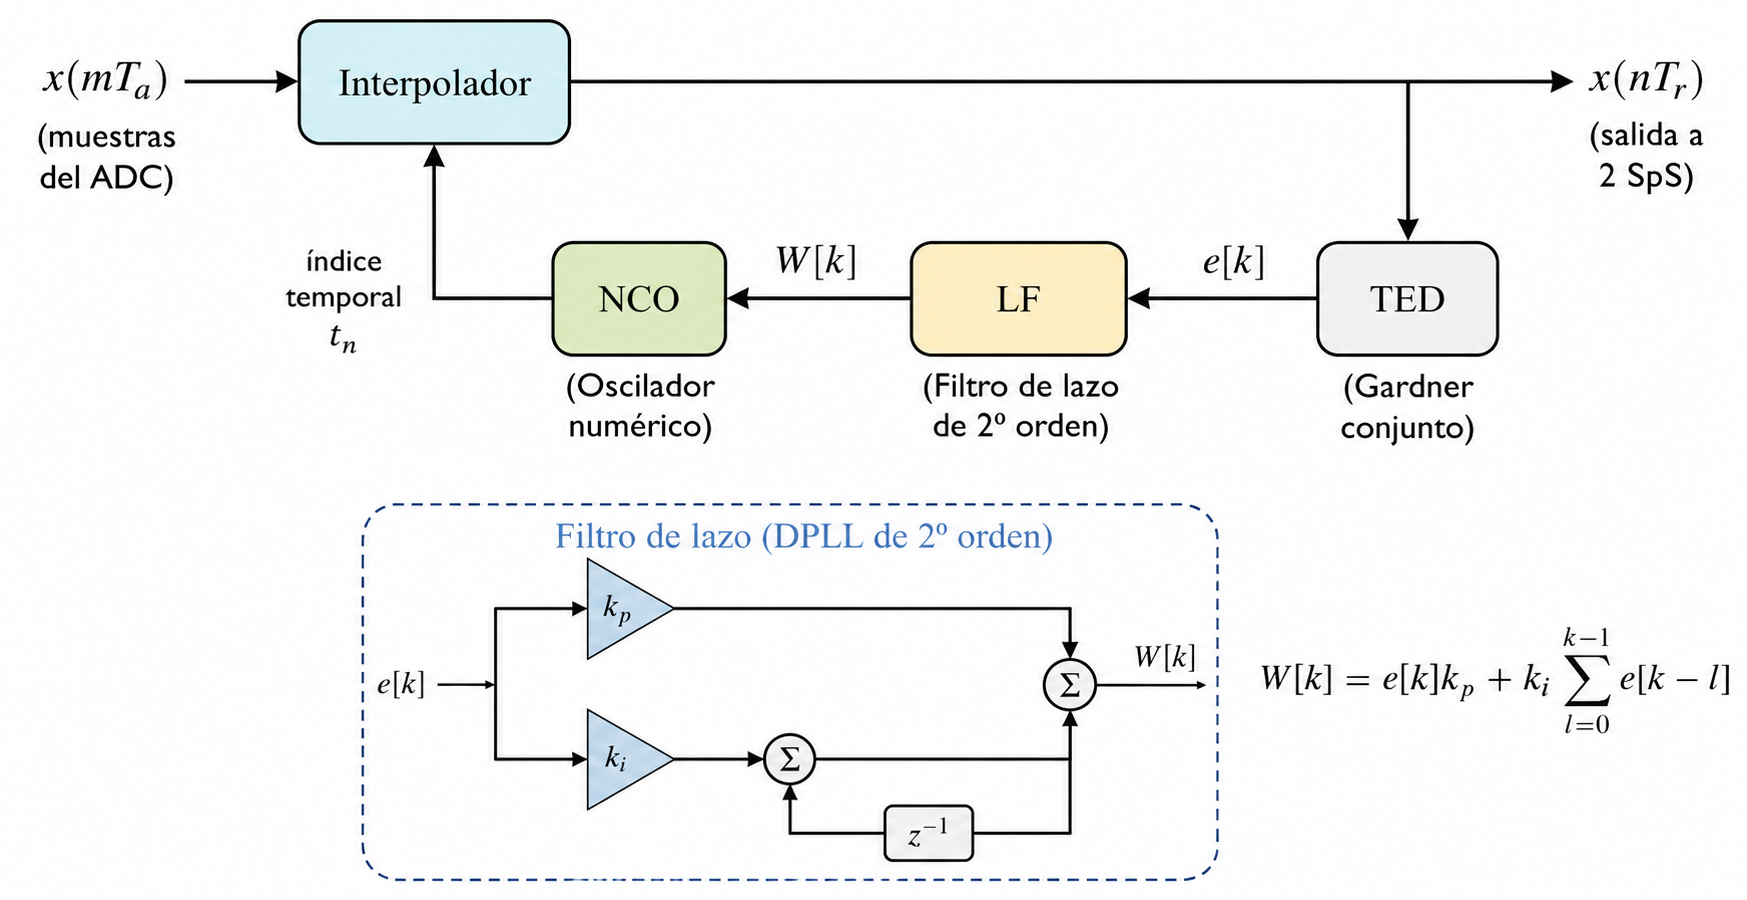
\includegraphics[width=\linewidth]{ClockRecoveryDiagrama2}
  \caption[Lazo de recuperaci\'on de reloj]{%
    Recuperaci\'on de reloj: interpolador controlado por un lazo cerrado. El
    detector de error de tiempo (TED) mide cu\'anto se aparta el instante de
    muestreo del \'optimo, el filtro de lazo PI integra el error y el
    oscilador num\'erico (NCO) produce el \'indice temporal $t_n$ con el que el
    interpolador reconstruye la muestra. Abajo, el filtro de lazo: rama
    proporcional $k_p$, rama integral $k_i$ con su acumulador.}
  \label{fig:clock}
\end{figure}

La \cref{fig:clock} muestra los tres elementos del lazo. El detector de error
de tiempo mide cu\'anto se aparta el instante de muestreo del \'optimo, el
filtro proporcional-integral promedia el error, y el oscilador num\'erico
acumula el resultado para producir el \'indice temporal con el que el
interpolador reconstruye cada muestra.

\paragraph{Detector de error de tiempo}
Se implementa el detector de Gardner~\cite{gardner1986}, que opera a dos muestras por
s\'imbolo. Toma el centro del s\'imbolo actual, el del anterior y la muestra
intermedia, que idealmente cae en el cruce por cero, y calcula
\begin{equation}
  e[k] = \Re\!\left\{\left(x_k - x_{k-1}\right)\, x_{k-1/2}^{*}\right\}.
  \label{eq:gardner}
\end{equation}
Si el muestreo est\'a en el instante \'optimo, el pulso es sim\'etrico
alrededor del cruce, la muestra intermedia cae en cero y el producto se anula.
Si est\'a adelantado o atrasado, la muestra intermedia toma un valor no nulo
cuyo signo indica la direcci\'on del desv\'io. El factor $(x_k - x_{k-1})$
aporta la direcci\'on de la transici\'on, de modo que el signo del error no
dependa de qu\'e s\'imbolos se hayan transmitido. El error se suma sobre las
dos polarizaciones, $e[k] = e_V[k] + e_H[k]$, para que un desvanecimiento en
una de ellas no deje al lazo sin se\~nal.

\paragraph{Interpolador}
La reconstrucci\'on usa un interpolador c\'ubico sobre las cuatro muestras
adyacentes al instante deseado.

\paragraph{Par\'ametros del lazo}
El filtro de lazo es proporcional-integral, as\'i que el conjunto
TED\,--\,filtro\,--\,NCO constituye un lazo de segundo orden, o de tipo~2. Sus
par\'ametros can\'onicos son~\cite[ec.~(7.10)--(7.12)]{mello2021}
\begin{equation}
  \omega_n T = \sqrt{k_i K_d},
  \qquad
  \zeta = \frac{k_p}{2}\sqrt{\frac{K_d}{k_i}},
  \qquad
  B_L = \frac{\omega_n}{2}\left(\zeta + \frac{1}{4\zeta}\right).
  \label{eq:lazo-2do}
\end{equation}
Ac\'a $k_p$ y $k_i$ son las ganancias de las ramas proporcional e integral del
filtro, $K_d$ es la sensibilidad del detector, $T = 1/\Rs$ el per\'iodo de
s\'imbolo, $\omega_n$ la frecuencia natural del lazo, $\zeta$ su factor de
amortiguamiento y $B_L$ su ancho de banda de ruido unilateral. Este \'ultimo
es el que gobierna el compromiso entre seguir variaciones r\'apidas del reloj
y filtrar el ruido.

Combinando las dos primeras expresiones se obtiene $\omega_n\zeta = k_p K_d/(2T)$
y $\omega_n/(4\zeta) = k_i/(2 k_p T)$, de modo que las ra\'ices se cancelan y
el ancho de banda queda en forma cerrada,
\begin{equation}
  B_L = \frac{\Rs}{4}\left( k_p K_d + \frac{k_i}{k_p} \right).
  \label{eq:BL-cerrada}
\end{equation}
La rama proporcional entra multiplicada por la ganancia del detector y la
integral dividida por la proporcional.

La sensibilidad $K_d$ es la pendiente de la curva caracter\'istica del
detector en el origen, que se obtiene de la \cref{tab:gardner-beta} m\'as
adelante. Para $\beta = 0{,}2$ vale \num{0.63}. Con $k_p = \num{e-3}$ y
$k_i = \num{e-7}$ se tiene
\begin{equation}
  f_n = \frac{\omega_n}{2\pi} = \SI{1.28}{\mega\hertz},
  \qquad
  \zeta = \num{1.25},
  \qquad
  B_L = \SI{5.8}{\mega\hertz}.
  \label{eq:lazo-reloj}
\end{equation}
Con $\zeta > 1$ el lazo queda sobreamortiguado, sin sobrepico. Su tiempo de
respuesta, estimado como $1/(2B_L)$, es de \SI{86}{\nano\second}, lo que a
\SI{32}{\giga\baud} se corresponde con unos \num{2750} s\'imbolos.

\paragraph{L\'imites del lazo}
De estos par\'ametros surgen tres consecuencias para el enlace.

\begin{itemize}

\item \textbf{Desv\'io constante de la tasa de muestreo:} Un lazo de tipo~2
sigue una rampa de fase sin dejar error en r\'egimen permanente, de modo que
el desv\'io de \SI{25.55}{\ppm} que impone el Doppler
(\cref{sec:canal-doppler}) queda compensado por completo. Ese desv\'io
equivale a una deriva del instante de muestreo de \SI{8.2e5}{} s\'imbolos por
segundo, que la rama integral alcanza en unos \num{250} s\'imbolos, dentro de
la ventana de entrenamiento del ecualizador.

\item \textbf{Aceleraci\'on:} Lo que un lazo de tipo~2 s\'i deja como error
est\'atico es la variaci\'on del desv\'io. La aceleraci\'on radial del pase,
$a_r = \SI{10.15}{\meter\per\second\squared}$, hace variar la tasa a raz\'on
de $a_r/c = \SI{3.4e-8}{\per\second}$, lo que en el instante de muestreo
representa una aceleraci\'on de \num{1083} s\'imbolos por segundo al cuadrado.
El error residual que deja es
\begin{equation}
  \tau_{ss} = \frac{\ddot\tau}{\omega_n^2}
            = \SI{1.7e-11}{}\ \text{s\'imbolos},
  \label{eq:error-acel}
\end{equation}
despreciable frente al per\'iodo de s\'imbolo.

\item \textbf{Deslizamiento de s\'imbolo:} La curva caracter\'istica del
detector no tiene un \'unico cero, y de ah\'i surge el tercer l\'imite.

\begin{figure}[H]
  \centering
  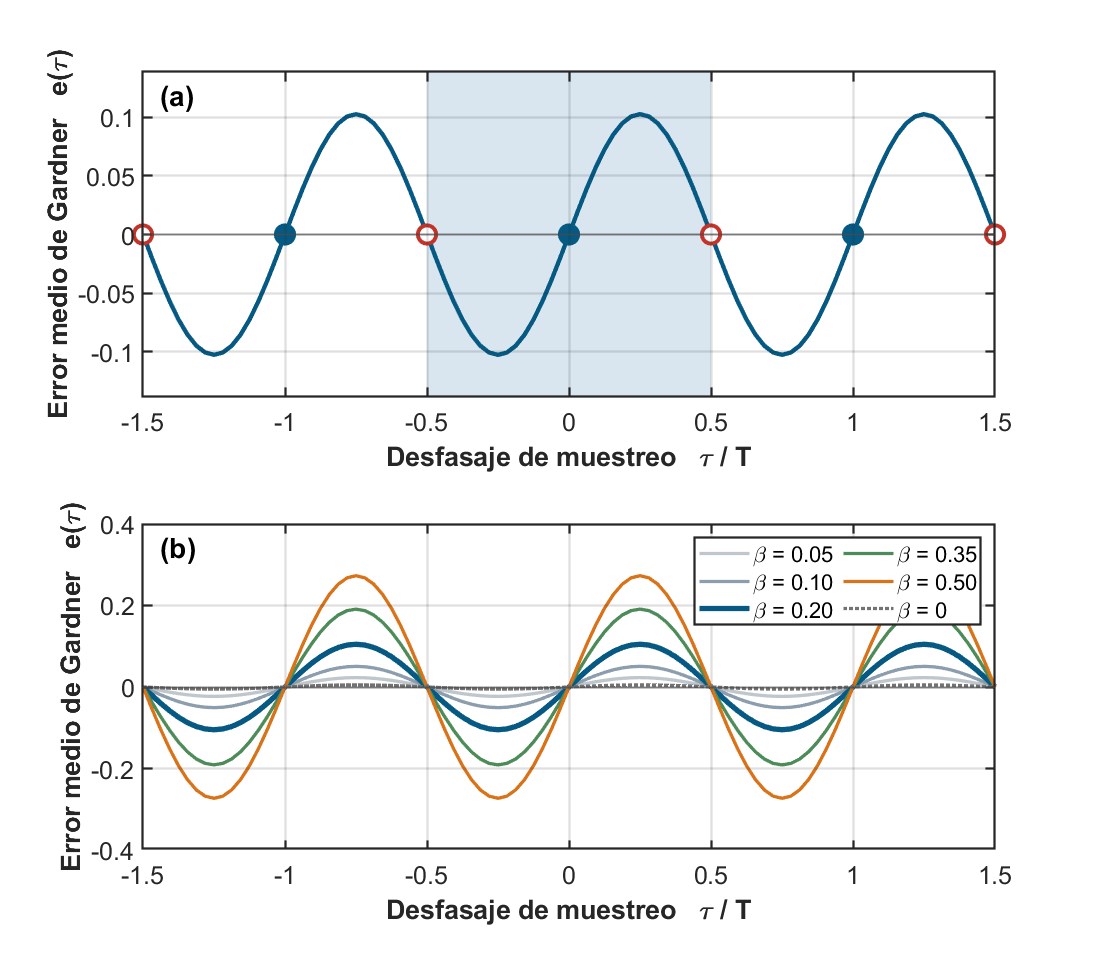
\includegraphics[width=0.92\linewidth]{gardner_scurve}
  \caption[Curva caracter\'istica del detector de Gardner]{%
    Error medio del detector de Gardner en funci\'on del desfasaje de muestreo
    $\tau$, obtenido promediando la \cref{eq:gardner} sobre \num{2e4}
    s\'imbolos QPSK conformados con el par RRC transmisor--receptor.
    \textbf{(a)} Con $\beta = 0{,}2$: la curva completa un ciclo por s\'imbolo.
    Los c\'irculos llenos marcan los puntos de enganche, separados $T$ entre
    s\'i, y los vac\'ios, los cruces intermedios, donde el error tambi\'en se
    anula pero el lazo es inestable. La franja sombreada tiene ancho $T$ y es
    el intervalo de captura alrededor de un punto de enganche.
    \textbf{(b)} El mismo barrido para varios \emph{roll-off}. La amplitud, y
    con ella la pendiente en el origen, se reducen a cero al disminuir $\beta$.}
  \label{fig:gardner-scurve}
\end{figure}

La \cref{fig:gardner-scurve} muestra el error medio del detector en funci\'on
del desfasaje de muestreo. Como se ve en el panel~(a), la curva es
peri\'odica con per\'iodo $T = 1/\Rs = \SI{31.25}{\pico\second}$, es decir que
el detector completa un ciclo entero por cada s\'imbolo que se corre el
instante de muestreo.

La consecuencia es que el punto de enganche no es \'unico. El error se anula
cada $T/2$, alternando el signo de la pendiente. Los cruces con pendiente de
un signo son puntos de equilibrio estable, porque ante una perturbaci\'on el
error realimentado empuja al lazo de vuelta hacia ellos, y los intermedios son
inestables por la raz\'on opuesta. Los estables est\'an separados $T$ entre
s\'i y el detector entrega el mismo error en todos, de modo que el lazo no
dispone de informaci\'on para distinguirlos. Son todos v\'alidos y difieren en
un s\'imbolo entero.

Eso define un intervalo de captura de $\pm T/2$ alrededor de cada punto de
enganche, que es el \'area sombreada de la figura. Si una perturbaci\'on
desplaza al lazo m\'as all\'a de esa franja antes de que alcance a corregirla,
el lazo converge al punto de enganche vecino y la salida queda corrida un
s\'imbolo entero. Cu\'an r\'apido puede el lazo absorber esa perturbaci\'on lo
determina $B_L$.

\item \textbf{Dependencia con el \emph{roll-off}.} La sensibilidad del
detector depende del conformado del pulso. La informaci\'on de temporizado de
una se\~nal modulada linealmente no est\'a en su espectro de potencia sino en
la correlaci\'on entre componentes separadas $\Rs$, y con un RRC esa
correlaci\'on solo existe en la banda de transici\'on del filtro, de ancho
$\beta\Rs$ a cada lado~\cite{franks1980}. Con $\beta = 0{,}2$ son
\SI{6.4}{\giga\hertz} de cada lado. Al reducir el \emph{roll-off} esa banda se
angosta, hasta que en $\beta = 0$ desaparece y no queda informaci\'on de
temporizado.

\begin{table}[htbp]
  \centering
  \begin{tabular}{ccc}
    \toprule
    $\beta$ & $\abs{K_d}$ & respecto de $\beta = 0{,}2$ \\
    \midrule
    \num{0}    & \num{0.029} & \SI{5}{\percent} \\
    \num{0.05} & \num{0.148} & \SI{24}{\percent} \\
    \num{0.10} & \num{0.337} & \SI{54}{\percent} \\
    \num{0.20} & \num{0.628} & \SI{100}{\percent} \\
    \num{0.35} & \num{1.177} & \SI{187}{\percent} \\
    \num{0.50} & \num{1.746} & \SI{278}{\percent} \\
    \bottomrule
  \end{tabular}
  \caption[Ganancia del detector de Gardner contra el \emph{roll-off}]{%
           Ganancia del detector de Gardner contra el \emph{roll-off},
           medida como la pendiente de la curva S en el origen.}
  \label{tab:gardner-beta}
\end{table}

La \cref{tab:gardner-beta} cuantifica esa dependencia. $K_d$ crece de manera
aproximadamente proporcional a $\beta$, y en $\beta = 0$ la pendiente es dos
\'ordenes de magnitud menor que en el valor adoptado. Seg\'un la
\cref{eq:lazo-2do}, $\omega_n$ y $\zeta$ escalan con $\sqrt{K_d}$, de modo que
bajar el \emph{roll-off} vuelve al lazo m\'as lento y peor amortiguado. Esta
es una de las razones por las que no se redujo $\beta$ por debajo de
\num{0.2}.

\end{itemize}


\section{Ecualizaci\'on adaptativa MIMO}
\label{sec:dsp-ddlms}

\paragraph{Prop\'osito}
Esta funci\'on se encarga de compensar la mezcla din\'amica de las dos
polarizaciones que introduce la rotaci\'on del estado de polarizaci\'on a lo
largo del enlace, la interferencia entre s\'imbolos residual y el skew
temporal entre ramas.

\paragraph{Principio de operaci\'on}
El ecualizador es una estructura mariposa $2\times2$. Cada salida es la suma
de dos filtros FIR aplicados a las dos entradas,
\begin{equation}
  \begin{bmatrix} y_X[k] \\ y_Y[k] \end{bmatrix}
  =
  \begin{bmatrix} \mathbf{h}_{XX} & \mathbf{h}_{XY} \\
                  \mathbf{h}_{YX} & \mathbf{h}_{YY} \end{bmatrix}
  \begin{bmatrix} \mathbf{x}_X[k] \\ \mathbf{x}_Y[k] \end{bmatrix},
  \label{eq:mariposa}
\end{equation}
con \num{7} coeficientes por rama y espaciado fraccionado $T/2$. La entrada
llega a dos muestras por s\'imbolo y la salida se entrega a una. Ese espaciado
fraccionado es lo que le permite corregir retardos de una fracci\'on de
s\'imbolo, es decir el skew.

\begin{figure}[H]
  \centering
  \makebox[\linewidth][c]{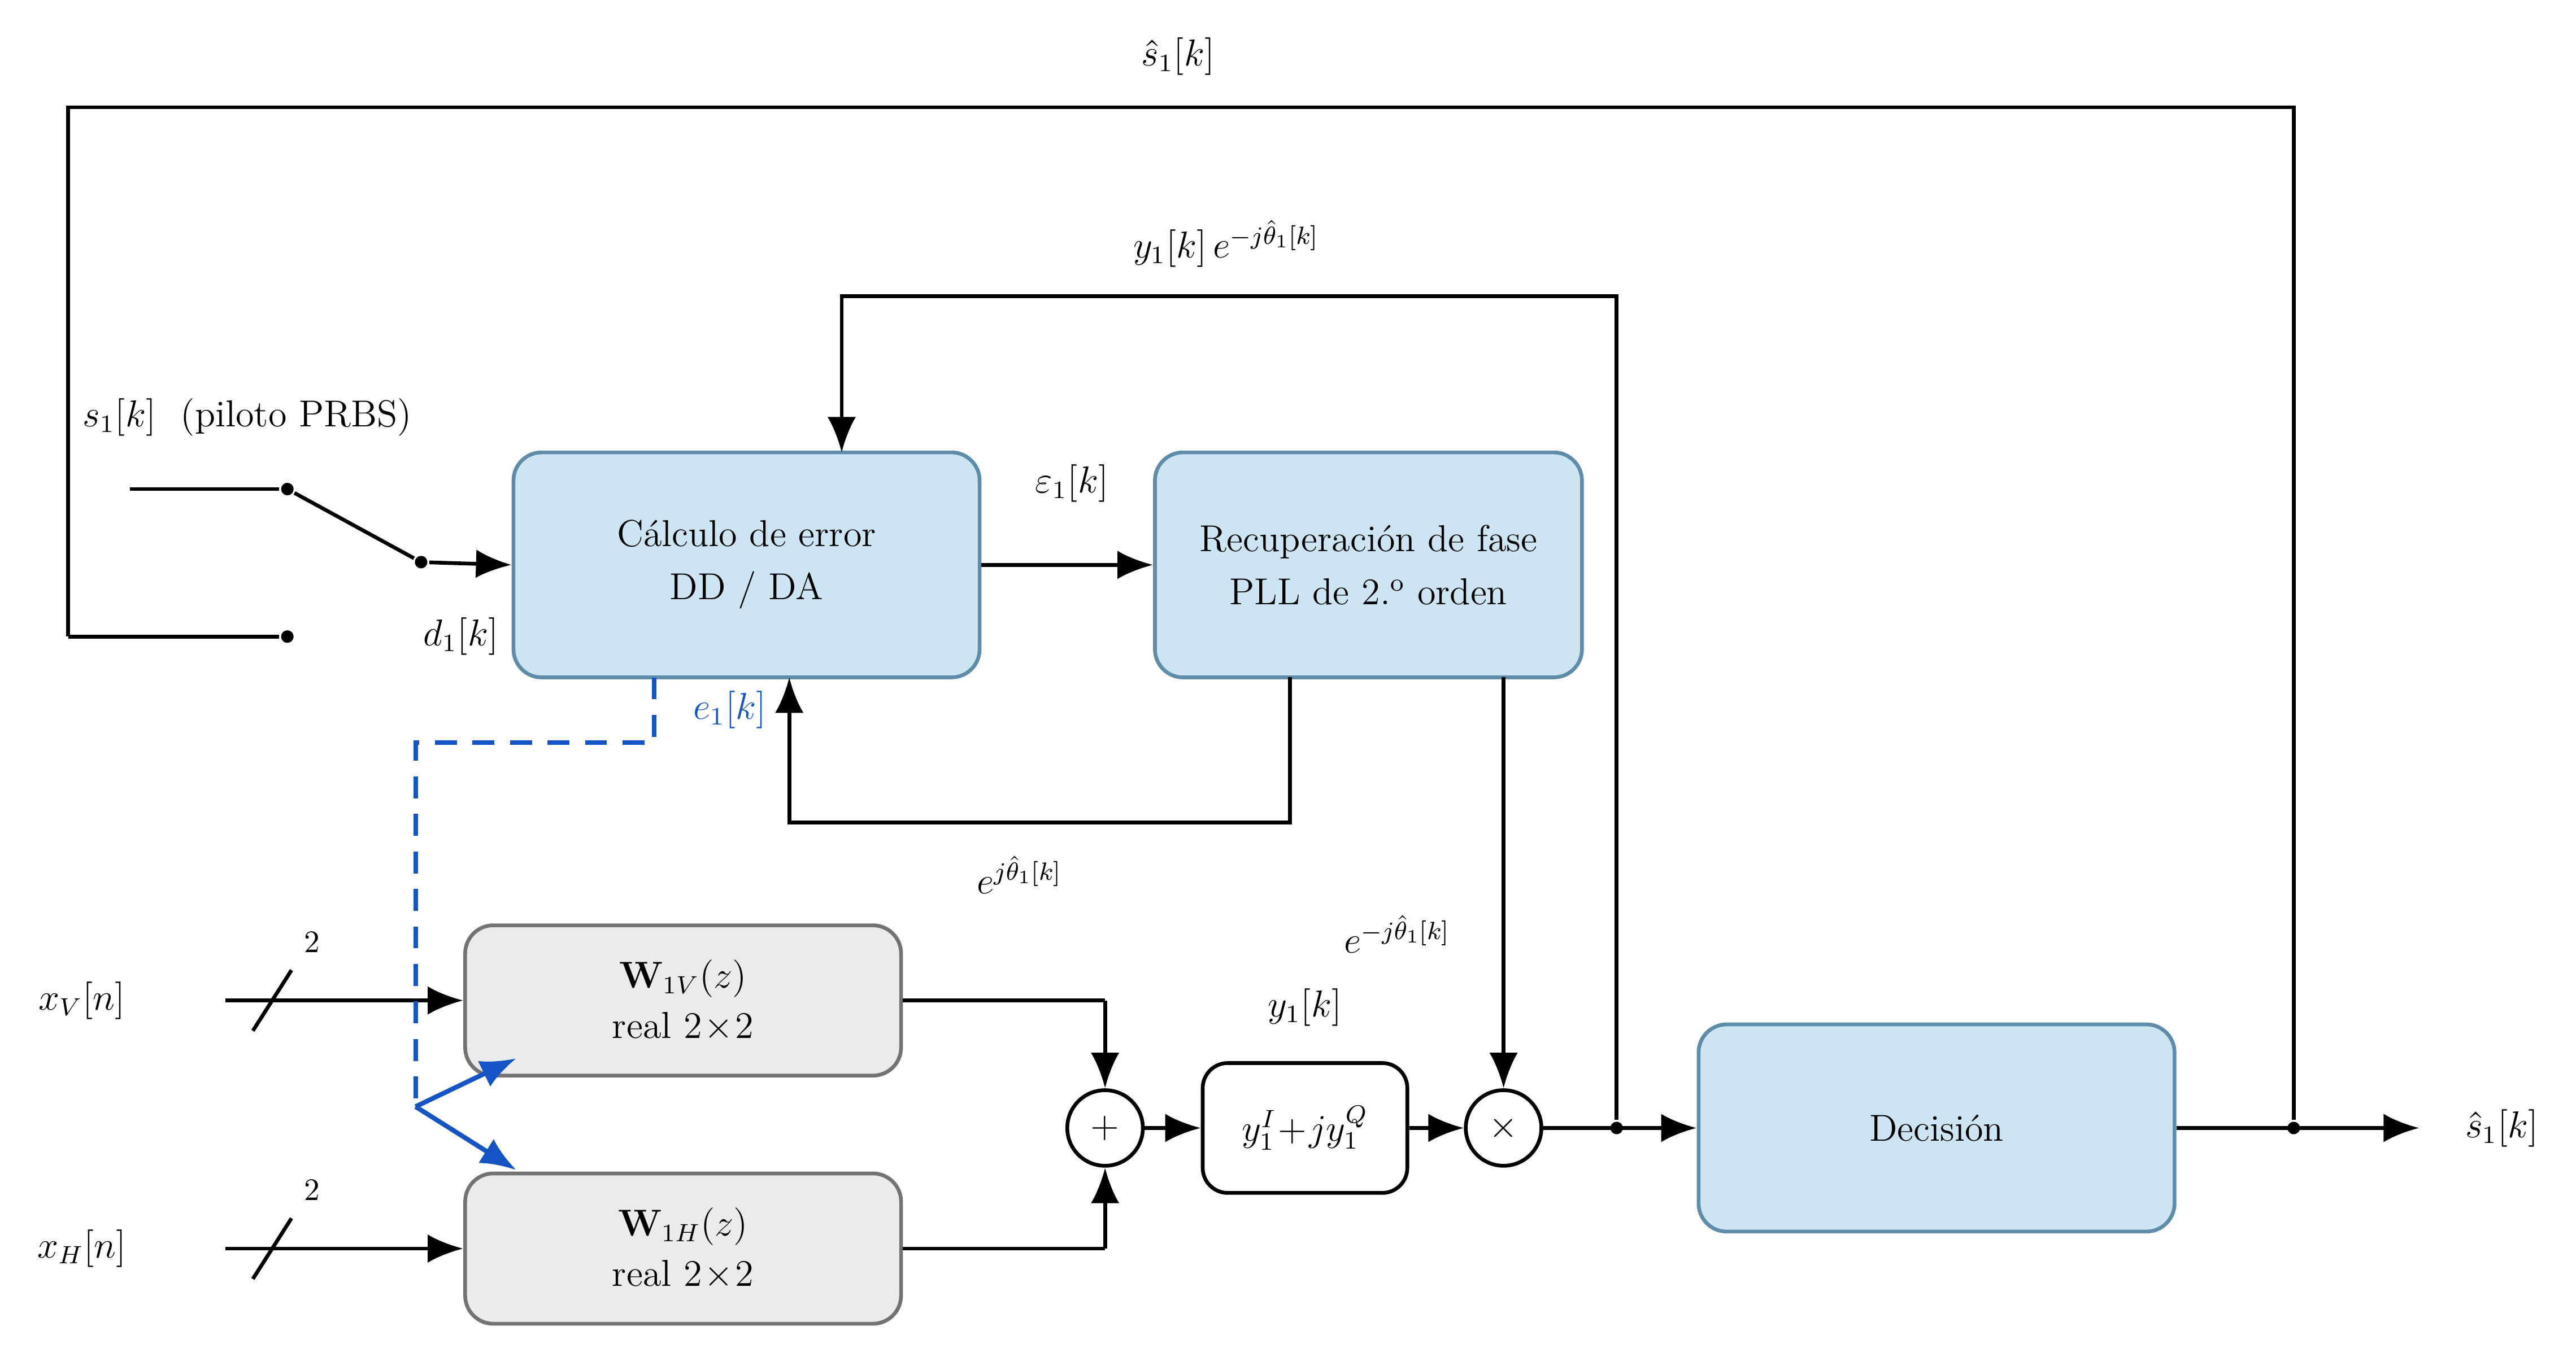
\includegraphics[width=1.12\linewidth]{ddlms_real_pol1_3}}
  \caption[Ecualizador mariposa y lazo de fase]{%
    Rama del ecualizador que genera la polarizaci\'on~V. Las dos entradas
    $x_V[n]$ y $x_H[n]$ llegan a \num{2} muestras por s\'imbolo, cada una pasa
    por su matriz real de $2\times2$ y las dos salidas se suman para formar
    $y_1[k]$ a una muestra por s\'imbolo. El conmutador de arriba a la
    izquierda selecciona la referencia del error: el piloto PRBS durante los
    primeros $N_{\mathrm{tr}}$ s\'imbolos y la propia decisi\'on despu\'es. La
    estructura es sim\'etrica, de modo que la rama que genera la
    polarizaci\'on~H es id\'entica, con sus propias $\mathbf{W}_{2V}$ y
    $\mathbf{W}_{2H}$ y su propio lazo de fase.}
  \label{fig:ddlms}
\end{figure}

La \cref{fig:ddlms} muestra una de las dos ramas de la estructura, la que
genera la polarizaci\'on~V, con el lazo de fase de la \cref{sec:dsp-cpr} ya en
su lugar. La otra rama es id\'entica y opera en paralelo sobre las mismas dos
entradas. En el diagrama se observa c\'omo cada entrada atraviesa su propio
filtro antes de sumarse, y c\'omo el conmutador de la referencia del error
decide si el algoritmo se entrena contra el piloto o contra su propia
decisi\'on.

La regla de actualizaci\'on de los coeficientes del filtro es el gradiente
estoc\'astico del algoritmo LMS~\cite[sec.~5.2]{mello2021},
\begin{equation}
  \mathbf{h}(n+1) = \mathbf{h}(n) + \mu\, e(n)\, \mathbf{x}^{*}(n),
  \label{eq:lms}
\end{equation}
con un paso de adaptaci\'on $\mu = 0{,}01$. El error $e(n)$ se calcula de dos
maneras distintas. Durante los primeros $N_{\mathrm{tr}} = \num{1000}$
s\'imbolos se utiliza la referencia PRBS conocida, en el modo asistido por
datos. Despu\'es de esa etapa, el error se calcula contra la propia
decisi\'on, en el modo dirigido por decisi\'on.

Un detalle de implementaci\'on que se pierde en la notaci\'on compacta de la
\cref{eq:mariposa} es que cada rama $\mathbf{h}_{ij}$ no es un filtro complejo
sino una matriz real de $2\times2$ que act\'ua sobre el par
$[\,\mathrm{Re},\ \mathrm{Im}\,]$. Son \num{16} filtros FIR reales y no cuatro
complejos, y de ah\'i surgen dos capacidades que la notaci\'on no deja ver.

\begin{itemize}
  \item La matriz real de $2\times2$ permite aplicar ganancias distintas a las
        componentes en fase y en cuadratura y mezclar una en la otra, es
        decir, compensar la p\'erdida de ortogonalidad entre ramas. Un filtro
        estrictamente complejo, que multiplica por un solo n\'umero, no puede
        hacerlo.
  \item Como la entrada de esa matriz es un FIR de \num{7} coeficientes
        espaciados $T/2$, y no un escalar, el bloque puede aplicar retardos
        fraccionarios distintos a cada componente y compensar as\'i el skew.
\end{itemize}

Una regla alternativa para la actualizaci\'on de los coeficientes de forma
ciega es el algoritmo de m\'odulo constante
(CMA)~\cite[sec.~5.2.2]{mello2021}, que no necesita referencia. Para QPSK,
donde todos los s\'imbolos tienen el mismo m\'odulo, el CMA converge bien y es
la elecci\'on habitual en receptores comerciales. Ac\'a se opt\'o por DD-LMS
con arranque asistido por datos por dos motivos. El primero es que la
secuencia PRBS transmitida est\'a disponible, tanto en simulaci\'on como en la
validaci\'on experimental. El segundo es que el arranque asistido evita las
convergencias degeneradas que el CMA presenta cuando la mezcla de
polarizaciones est\'a cerca de la singularidad, y que de otro modo obligan a
una inicializaci\'on espec\'ifica de los coeficientes.

\paragraph{Seguimiento del estado de polarizaci\'on}
El ecualizador adaptativo sigue las variaciones temporales del canal con
cierto retraso. La velocidad de convergencia del algoritmo LMS depende del
paso de adaptaci\'on $\mu$ y de las propiedades estad\'isticas de la se\~nal
de entrada. En una aproximaci\'on simplificada, la constante de tiempo de
adaptaci\'on es del orden de $1/\mu$ s\'imbolos, equivalente a $1/(\mu\Rs)$
segundos. Por lo tanto, si el estado de polarizaci\'on rota a una velocidad
angular $\dot\theta$, el retraso del ecualizador se traduce en un error
angular de seguimiento del orden de $\dot\theta/(\mu\Rs)$.

Este comportamiento responde al compromiso del LMS frente a un sistema
variable en el tiempo. Reducir $\mu$ disminuye el exceso de error asociado al
ruido de gradiente, pero aumenta el error de seguimiento de las variaciones
del canal. Aumentar $\mu$, por el contrario, permite seguir variaciones m\'as
r\'apidas a costa de un mayor error en r\'egimen permanente. Este compromiso
se estudia en Haykin~\cite{haykin2014} y, en el contexto de receptores
\'opticos coherentes, en Savory~\cite{savory2010}. En la \cref{sec:tol-sop} se
analiza mediante un barrido del paso de adaptaci\'on, del que se obtiene un
valor adecuado de $\mu$.


\section{Recuperaci\'on de fase de portadora}
\label{sec:dsp-cpr}

\paragraph{Prop\'osito}
Compensa el ruido de fase de los l\'aseres, tanto del transmisor como del
oscilador local, y el residuo de frecuencia que deja el estimador de la
\cref{sec:dsp-frec}. Es el bloque que fija la tolerancia al ruido de fase de los l\'aseres transmisor
y receptor.

\paragraph{Principio de operaci\'on}
Es un lazo de segundo orden integrado al ecualizador que utiliza el mismo
error de decisi\'on que este \'ultimo (\cref{fig:pll}). El detector compara la
se\~nal con la decisi\'on y devuelve el error de fase,
\begin{equation}
  \varepsilon[k] = \arg\!\left(y[k]\, d^{*}[k]\right).
  \label{eq:pll-detector}
\end{equation}
El filtro de lazo acumula ese error,
\begin{equation}
  u[k] = u[k-1] + g_1\left[(1+g_2)\,\varepsilon[k] - \varepsilon[k-1]\right],
  \label{eq:pll-filtro}
\end{equation}
y el oscilador controlado num\'ericamente acumula la correcci\'on,
\begin{equation}
  \hat\theta[k+1] = \hat\theta[k] + u[k].
  \label{eq:pll-nco}
\end{equation}

\begin{figure}[H]
  \centering
  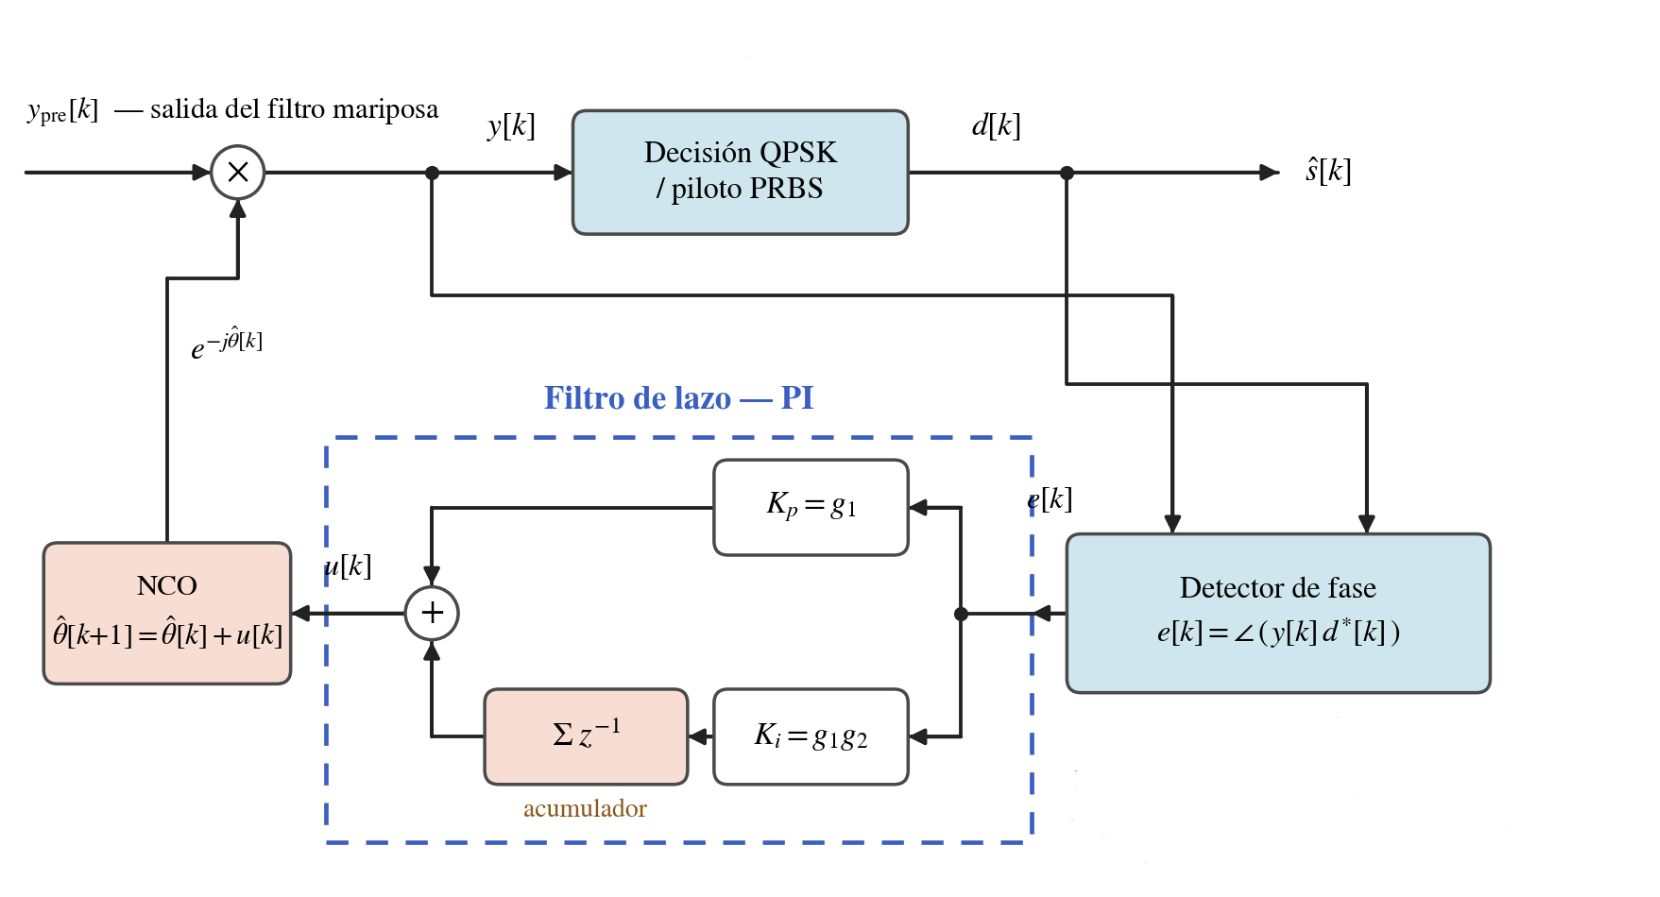
\includegraphics[width=0.95\linewidth]{ddlms_pll_recuperacionDeFase}
  \caption[Lazo de recuperaci\'on de fase]{%
    El lazo de fase dentro del bloque del ecualizador. La entrada
    $y_{\mathrm{pre}}[k]$ es la salida del filtro mariposa. El detector compara
    la se\~nal ya rotada contra la decisi\'on, que es el piloto PRBS durante el
    entrenamiento y la decisi\'on QPSK despu\'es. El filtro PI integra el error
    y el NCO acumula la fase estimada. El ecualizador se actualiza con el mismo
    error.}
  \label{fig:pll}
\end{figure}

Una alternativa a este lazo es un estimador feedforward tipo
Viterbi--Viterbi~\cite{mello2021}, que no necesita una etapa de enganche. En este trabajo se opt\'o por el lazo cerrado porque comparte el
error de decisi\'on con el ecualizador. De ese modo la rotaci\'on ya est\'a
corregida cuando el LMS actualiza los coeficientes, de manera que el
ecualizador no tiene que seguir al ruido de fase. Separar los dos bloques lo
obligar\'ia a compensar tambi\'en esa rotaci\'on, con una convergencia m\'as
lenta.

\paragraph{L\'imite te\'orico del lazo}
La \cref{eq:pll-filtro} es la misma rama proporcional e integral del lazo de
reloj, escrita de otra forma. Si se la desarrolla,
\[
  g_1\left[(1+g_2)\,\varepsilon[k] - \varepsilon[k-1]\right]
  = g_1\left(\varepsilon[k]-\varepsilon[k-1]\right) + g_1 g_2\,\varepsilon[k],
\]
queda claro que $K_p = g_1$ y $K_i = g_1 g_2$. Como es un lazo de tipo~2,
valen las mismas expresiones de la \cref{eq:lazo-2do}.

Como el error se calcula como $\arg(y\,d^{*})$, se tiene que $K_d = 1$. Con
$g_1 = 0{,}06$ y $g_2 = 0{,}025$, los parámetros característicos del lazo valen:
\begin{equation}
  f_n = \SI{197}{\mega\hertz},
  \qquad
  \zeta = \num{0.77},
  \qquad
  B_L = \SI{680}{\mega\hertz}.
  \label{eq:lazo-fase}
\end{equation}


\paragraph{Tolerancia al ancho de l\'inea}
El lazo no corrige la fase de forma instant\'anea. Su tiempo de respuesta
frente a un error de fase es del orden de
$\tau_L = 1/2B_L = \SI{0.74}{\nano\second}$. Lo que queda sin corregir en cada
instante es la fase que se acumul\'o durante los \'ultimos $\tau_L$ segundos.

La fase de un l\'aser es un proceso de Wiener, de modo que el incremento en un
intervalo $\tau$ es una variable aleatoria de media nula y varianza
proporcional a $\tau$. Para el ancho espectral combinado de los dos l\'aseres,
$\dnu_{\mathrm{tot}} = 2\dnu$,
\begin{equation}
  \sigma_\varphi^2
    = \operatorname{Var}\!\left[\varphi(t+\tau_L) - \varphi(t)\right]
    = 2\pi\, \dnu_{\mathrm{tot}}\, \tau_L
    = \frac{\pi\, \dnu_{\mathrm{tot}}}{B_L},
  \label{eq:var-fase}
\end{equation}
siendo entonces $\sigma_\varphi$ el valor eficaz del error de fase residual.

La \cref{eq:var-fase} contiene el compromiso de dise\~no del lazo. El error
residual crece con la ra\'iz del ancho de l\'inea y decrece con la ra\'iz del
ancho de banda del lazo. Ensanchar el lazo mejora el seguimiento de la fase,
pero tambi\'en deja entrar m\'as ruido aditivo al detector, efecto que esta
expresi\'on no contempla. El \'optimo surge al encontrar un equilibrio entre ambos mecanismos.

Mientras el error de fase instant\'aneo
se mantenga dentro del margen angular de QPSK, $\pm\ang{45}$
(\cref{cap:coherentes}), el lazo lo corrige. Cuando una excursi\'on lo supera,
el lazo se re-engancha desplazado un cuarto de vuelta y a partir de ah\'i
todos los s\'imbolos quedan decididos de manera err\'onea. Como el error de fase es gaussiano
de media nula, la frecuencia de esas excursiones es gobernada por la cantidad
de veces que cabe $\sigma_\varphi$ en los \ang{45}.

Esa ambig\"uedad de un m\'ultiplo de $\pi/2$ es tambi\'en la raz\'on por la
cual las m\'etricas se eval\'uan sobre las cuatro rotaciones posibles y sobre
el conjugado, tomando la de menor error.

El valor de $\sigma_\varphi$ al que se produce el quiebre no se deduce de
\eqref{eq:var-fase}, porque depende del presupuesto de error que el ruido
aditivo deja disponible. En el \cref{cap:tolerancias} se lo determina por
simulaci\'on, junto con el ancho de l\'inea m\'aximo tolerado y la ley de
escala con $B_L$.


\section{Sincronizaci\'on}
\label{sec:dsp-decision}

La cadena sincroniza la se\~nal recibida con la secuencia PRBS transmitida,
dos veces. La primera vez ocurre antes del ecualizador, para empezar la etapa
asistida por datos, y la segunda despu\'es, para poder comparar s\'imbolo a
s\'imbolo. Un receptor real no conoce la secuencia transmitida, as\'i que
estos dos bloques pertenecen al entorno de simulaci\'on y no a la cadena de recepci\'on. Por esa raz\'on
est\'an dibujados aparte en la \cref{fig:dsp-cadena}. Las m\'etricas se
calculan sobre los s\'imbolos posteriores a la ventana de convergencia del
ecualizador.

\section{Justificaci\'on del orden de los bloques}
\label{sec:dsp-orden}

\begin{itemize}

\item El ortogonalizador es el primer bloque porque compensa un error que se
vuelve irreversible si la recuperaci\'on de frecuencia act\'ua antes. Con
desbalance de cuadratura, la se\~nal compleja que se construye a partir de las
ramas, $z$, no es la deseada sino una combinaci\'on lineal en sentido amplio
de la se\~nal transmitida $s$ y de su conjugada,
\begin{equation}
  z = c_1\,s + c_2\,s^{*},
  \qquad
  c_1 = \tfrac{1}{2}\left(1 + \gamma e^{j\phi}\right),
  \qquad
  c_2 = \tfrac{1}{2}\left(1 - \gamma e^{j\phi}\right),
  \label{eq:iq-imbalance}
\end{equation}
donde $\gamma$ es el desbalance de ganancia entre I y Q y $\phi$ el
apartamiento de la cuadratura. El t\'ermino $c_2\,s^{*}$ es una imagen
conjugada. Si $s$ est\'a centrada en $+\Df$, la imagen est\'a en $-\Df$.

La imagen queda entonces exactamente en la frecuencia espejo de la se\~nal.
Eso es lo que permite cancelarla con una matriz real de $2\times2$ sin
memoria. El ortogonalizador aplica justamente eso, una operaci\'on
est\'atica sobre el par $(I, Q)$ con un solo par de coeficientes para toda la
se\~nal.

Ahora sup\'ongase que primero se corrige la frecuencia, es decir que se
multiplica todo por $e^{-j2\pi\Df t}$. Llamando $s' = s\,e^{-j2\pi\Df t}$ a la
se\~nal ya recentrada, y notando que
$s^{*}e^{-j2\pi\Df t} = s'^{*}\,e^{-j4\pi\Df t}$,
\begin{equation}
  z' = c_1\,s' + c_2\,s'^{*}\,e^{-j4\pi\Df t}.
  \label{eq:imagen-rotante}
\end{equation}
La imagen qued\'o en $-2\Df$ y dej\'o de estar en la frecuencia espejo. Una
matriz real de $2\times2$ sin memoria no puede cancelar un t\'ermino cuya fase
relativa rota. El ecualizador MIMO tampoco llega a seguirla. Sus coeficientes
se adaptan con una constante de tiempo de cien s\'imbolos, unos
\SI{3.1}{\nano\second}, mientras que la imagen completa una vuelta cada
\SI{0.25}{\nano\second} para el offset mayor de la \cref{tab:orden-gsop}.

El ortogonalizador tampoco puede estimar la correcci\'on en ese escenario.
Calcula un \'unico coeficiente de correlaci\'on $\E{r_I r_Q}$ promediado sobre
todo el bloque y aplica una \'unica correcci\'on est\'atica. Mientras la imagen
est\'a en el espejo, su aporte a esa correlaci\'on es un valor fijo y distinto
de cero. Cuando la imagen rota, el aporte promedia a cero y la estimaci\'on
falla.

La \cref{fig:orden-gsop} y la \cref{tab:orden-gsop} lo verifican en
simulaci\'on, inyectando un error de cuadratura conocido en los cuatro
carriles y comparando los dos \'ordenes con el resto de la cadena intacto.

\begin{figure}[H]
  \centering
  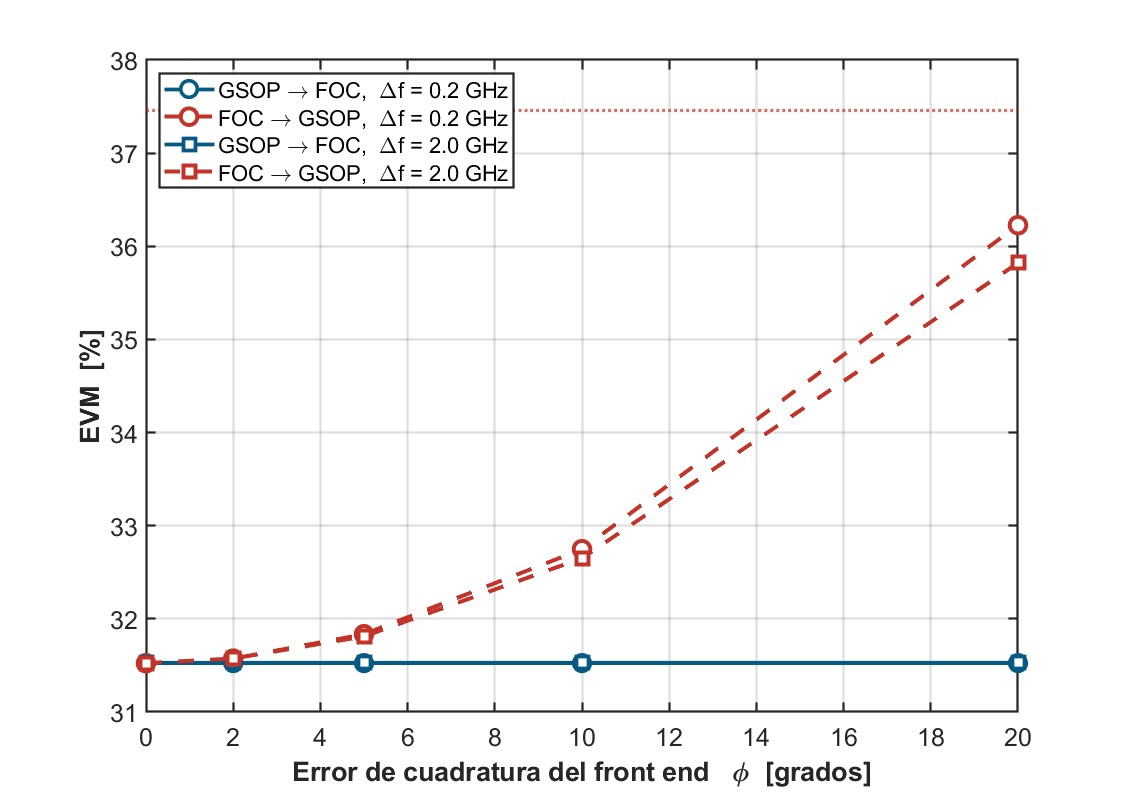
\includegraphics[width=0.92\linewidth]{orden_gsop_foc}
  \caption[Orden del ortogonalizador y el recuperador de frecuencia]{%
    EVM contra el error de cuadratura del front end, para los dos \'ordenes
    posibles y dos valores de offset de frecuencia. Con el orden correcto, en
    azul, las dos curvas quedan superpuestas y planas, de modo que el
    ortogonalizador remueve el desbalance por completo. Con el orden
    invertido, en rojo, el EVM crece con $\phi$. Las dos curvas quedan casi
    superpuestas entre s\'i aunque los offsets difieren un factor \num{10}, lo
    que muestra que la degradaci\'on no depende de $\Df$. La l\'inea punteada
    es el l\'imite HD-FEC.}
  \label{fig:orden-gsop}
\end{figure}

\begin{table}[H]
  \centering

  \begin{tabular}{cccccc}
    \toprule
    & \multicolumn{2}{c}{$\Df = \SI{0.2}{\giga\hertz}$}
    & \multicolumn{2}{c}{$\Df = \SI{2.0}{\giga\hertz}$} & \\
    \cmidrule(lr){2-3}\cmidrule(lr){4-5}
    $\phi$ & GSOP$\to$FOC & FOC$\to$GSOP & GSOP$\to$FOC & FOC$\to$GSOP
           & Penalidad \\
    \midrule
    \ang{0}  & \SI{31.52}{\percent} & \SI{31.52}{\percent} & \SI{31.53}{\percent} & \SI{31.53}{\percent} & \SI{0.00}{\dB} \\
    \ang{2}  & \SI{31.52}{\percent} & \SI{31.57}{\percent} & \SI{31.53}{\percent} & \SI{31.57}{\percent} & \SI{0.01}{\dB} \\
    \ang{5}  & \SI{31.52}{\percent} & \SI{31.83}{\percent} & \SI{31.53}{\percent} & \SI{31.81}{\percent} & \SI{0.09}{\dB} \\
    \ang{10} & \SI{31.52}{\percent} & \SI{32.75}{\percent} & \SI{31.53}{\percent} & \SI{32.65}{\percent} & \SI{0.33}{\dB} \\
    \ang{20} & \SI{31.52}{\percent} & \SI{36.23}{\percent} & \SI{31.53}{\percent} & \SI{35.82}{\percent} & \SI{1.21}{\dB} \\
    \bottomrule
  \end{tabular}
  \caption[Penalidad por invertir el orden de ortogonalizaci\'on y
           recuperaci\'on de frecuencia]{Penalidad por invertir el orden, a
           $\OSNR = \SI{14.4}{\dB}$ y \num{2e5} s\'imbolos.}
  \label{tab:orden-gsop}
\end{table}

Con el orden correcto el EVM es el mismo para todo $\phi$ entre \ang{0} y
\ang{20}, lo que indica que el ortogonalizador remueve el desbalance por
completo. Con el orden invertido el deterioro crece con $\phi$ hasta
\SI{1.21}{\dB}. La $\BER$ pasa de \num{7.6e-4} a \num{2.9e-3}, a un factor
\num{1.3} del umbral HD-FEC.

\item Por otro lado, hay una raz\'on para aplicar el filtro adaptado despu\'es
de la recuperaci\'on de frecuencia. El filtro RRC est\'a centrado en banda
base y tiene un ancho de banda de
$\Rs(1+\beta)/2 = \SI{19.2}{\giga\hertz}$. Con el Doppler del enlace la
se\~nal llega corrida hasta \SI{6}{\giga\hertz}, as\'i que un filtro aplicado
antes de corregir el offset recortar\'ia un borde del espectro de la se\~nal y
dejar\'ia pasar ruido por el otro. El estimador de cuarta potencia, en cambio,
no necesita que la se\~nal est\'e centrada. Trabaja sobre el espectro completo,
por lo que puede aplicarse primero. Recentrada la se\~nal, el filtro adaptado
act\'ua correctamente.

\item A su vez, el detector de error de muestreo mide la asimetr\'ia del pulso
en torno al instante de decisi\'on, de modo que trabaja mejor sobre el pulso
ya conformado por el filtro adaptado, con el ruido fuera de banda rechazado.
Pero adem\'as el detector calcula un producto entre muestras separadas medio
s\'imbolo y se queda con la parte real. Si la portadora todav\'ia gira a GHz,
esas muestras se comparan con fases distintas y el signo del error se vuelve
aleatorio. El detector necesita entonces las dos cosas, el pulso conformado y
la se\~nal ya recentrada en continua. Ubicarlo a continuaci\'on del filtro
adaptado, que a su vez va despu\'es de la recuperaci\'on de frecuencia,
satisface las dos condiciones.

\item Por \'ultimo, el ecualizador MIMO adaptativo es el \'unico bloque que
necesita una decisi\'on correcta para actualizarse. Todo lo que pueda
compensarse con un algoritmo que no dependa de la decisi\'on, es decir el
desbalance, el offset de frecuencia, el ruido fuera de banda y la fase de
muestreo, se remueve antes. As\'i el ecualizador arranca desde una
constelaci\'on ya reconocible y no tiene que converger a ciegas.

\end{itemize}

\section{Conclusiones}
\label{sec:dsp-conclusiones}

En este cap\'itulo se describieron los algoritmos de procesamiento digital
del receptor. Cada uno compensa una degradaci\'on distinta de las que el
enlace LEO--GEO y el front end introducen sobre la se\~nal.


El resultado central del cap\'itulo es el l\'imite de captura del estimador de
frecuencia. De los tres mecanismos analizados, el que predomina es el plegado
de Nyquist del tono de cuarta potencia, fijando un rango de $\Rs/4 = \SI{8}{\giga\hertz}$. Contra el requerimiento de \SI{6.0}{\giga\hertz} del \cref{cap:canal}
queda un \SI{33}{\percent} de margen.

Los dos lazos cerrados quedaron caracterizados por sus par\'ametros de segundo
orden. El de reloj,  por ser de tipo~2, sigue el desv\'io de frecuencia de muestreo 
debido al Doppler sin error
est\'atico. La aceleraci\'on del pase
le deja un error residual despreciable. El lazo de fase, a su vez, deja un
error de fase residual que escala como $\sqrt{\dnu_{\mathrm{tot}}/B_L}$.

El ecualizador MIMO cierra la cadena y absorbe los efectos que los dem\'as bloques
dejan. Al implementarse con filtros reales fraccionados en $T/2$, tiene la capacidad de compensar
el skew entre ramas y el desbalance de cuadratura residual, dos efectos que una
estructura estrictamente compleja no puede corregir. Su necesidad no depende del
canal. Entre los dos filtros RRC se interponen las respuestas del front end y
del conversor, de manera que el par transmisor--receptor no cumple el criterio
de Nyquist y deja interferencia entre s\'imbolos aun con el enlace ideal.

El orden en que se ejecutan no es arbitrario. La ortogonalizaci\'on se posiciona primero
porque el desbalance de cuadratura genera una imagen conjugada que, una vez
que la recuperaci\'on de frecuencia recentra la se\~nal, pasa a rotar y deja
de ser corregible con una operaci\'on est\'atica. El filtro adaptado se sit\'ua
despu\'es de la recuperaci\'on de frecuencia porque est\'a centrado en continua y
recortar\'ia una se\~nal desplazada en gigahertz. El detector de error de
muestreo le sigue filtro adaptado, que le entrega el pulso ya
conformado y sin el ruido fuera de banda. El ecualizador es el \'ultimo bloque porque es
el \'unico bloque que necesita una decisi\'on correcta para adaptarse. La
simulaci\'on confirma el primero de esos argumentos, con una penalidad de
\SI{1.21}{\dB} al invertir el orden frente a un error de cuadratura de
\ang{20}.

El \cref{cap:tolerancias} cuantifica por simulaci\'on los m\'argenes que este
cap\'itulo dej\'o planteados, entre ellos el ancho de l\'inea m\'aximo
tolerado y la velocidad de rotaci\'on del estado de polarizaci\'on que el
ecualizador alcanza a seguir.
% !TeX root = ../main.tex
\chapter{Balance de potencia del enlace}
\label{cap:enlace}

\section{Introducci\'on}
\label{sec:enl-intro}

Los cap\'itulos anteriores desarrollaron por separado los tres bloques
fundamentales del enlace LEO--GEO. El modelo del canal y su principal fuente de
ruido (\cref{cap:canal}), el modelo del transmisor y el receptor \'opticos
(\cref{cap:transceptor}) y el procesamiento digital que compensa las
imperfecciones de los dos anteriores (\cref{cap:dsp}). Este cap\'itulo los
re\'une para analizar la viabilidad del enlace en t\'erminos de potencia.

Se realiza un balance de potencia donde se identifican las ganancias y las
p\'erdidas de cada etapa, y se establece una relaci\'on entre la potencia del
l\'aser transmisor y la OSNR a la entrada del receptor. Con los resultados de
simulaci\'on de la cadena completa se cuantifican las penalidades respecto del
l\'imite te\'orico de un receptor ideal en un canal AWGN, y se determina el
umbral de operaci\'on del sistema.

El cap\'itulo cierra con las simplificaciones del balance y con los t\'erminos
que quedaron fuera por el alcance del proyecto.
\section{Balance de potencia}
\label{sec:enl-linkbudget}

En el \cref{ap:ruido} se desarrolla el an\'alisis te\'orico que determina la
OSNR m\'inima necesaria para alcanzar el umbral de BER del esquema de
correcci\'on de errores. Para el sistema DP-QPSK de este trabajo ese requisito
es de \SI{12.61}{\dB}, suponiendo un receptor ideal sobre un canal AWGN. A
partir de ah\'i, el balance de potencia recorre las ganancias y las p\'erdidas
de cada etapa para determinar qu\'e potencia \'optica tiene que entregar el
l\'aser transmisor.

\paragraph{Relaci\'on entre potencia de l\'aser y OSNR:}
Sea $\Pcw$ la potencia \'optica emitida por el l\'aser transmisor, medida a la
entrada del modulador. El modulador DP introduce p\'erdidas por la conversi\'on
intr\'inseca de los MZM, por el acoplamiento a fibra y por la propagaci\'on a
trav\'es de las gu\'ias de onda y el rotador de polarizaci\'on. Para los
c\'alculos que siguen se tom\'o como referencia el modulador de niobato de
litio del laboratorio, que a \SI{32}{\giga\baud} especifica una p\'erdida de
inserci\'on total de hasta
\begin{equation}
  L_{\mathrm{DP}} = \SI{14}{\dB}
  \label{eq:liqm}
\end{equation}
seg\'un su hoja de datos~\cite{fujitsu_ftm7977}.

Considerando la ganancia del amplificador \'optico de transmisi\'on,
$G_b = \SI{35}{\dB}$, y la p\'erdida neta del enlace de la
\eqref{eq:pathloss}, la potencia \'optica a la entrada del pre-amplificador del
receptor resulta
\begin{equation}
  P_{rx} = \Pcw - L_{\mathrm{DP}} + G_b - L = \Pcw - \SI{52.40}{\dB}.
  \label{eq:prx}
\end{equation}

A la salida del pre-amplificador la potencia de se\~nal es
$P_{rx} + G_{\mathrm{EDFA}}$. La potencia total de ruido ASE que la acompa\~na
en el ancho de referencia es
$P_{\mathrm{ASE}} = 10\log_{10}\!\left(2S_{\mathrm{pol}}\Bref/\SI{1}{\milli\watt}\right)
= \SI{-28.46}{\dBm}$, con $S_{\mathrm{pol}}$ la densidad espectral de potencia
de ruido por cada uno de los dos modos de polarizaci\'on, definida en la
\eqref{eq:ase}. El cociente entre ambas potencias es la OSNR de la
\eqref{eq:osnr-def},
\begin{equation}
  \OSNR\,[\si{\dB}]
    = \underbrace{\left(P_{rx} + G_{\mathrm{EDFA}}\right)}_{\text{se\~nal en }\si{\dBm}}
      - \underbrace{P_{\mathrm{ASE}}}_{\text{ASE en }\si{\dBm}}
    = \Pcw\,[\si{\dBm}] - 52{,}40 + 25{,}0 + 28{,}46,
  \label{eq:osnr-pcw-pasos}
\end{equation}
que se reduce a una \'unica constante aditiva,
\begin{equation}
  \OSNR\,[\si{\dB}] = \Pcw\,[\si{\dBm}] + 1{,}06.
  \label{eq:osnr-pcw}
\end{equation}
Los dos t\'erminos que se restan en la \eqref{eq:osnr-pcw-pasos} est\'an en
\si{\dBm}, de modo que su diferencia es un cociente y queda en \si{\dB}. La
constante de la \eqref{eq:osnr-pcw} va sin unidad porque arrastra esa
cancelaci\'on de la referencia de \SI{1}{\milli\watt}.

Esta expresi\'on vincula el balance con las simulaciones del
\cref{cap:tolerancias}. Fijar una OSNR objetivo equivale a fijar la potencia
\'optica que tiene que entregar el l\'aser transmisor.

\begin{figure}[H]
  \centering
  \begin{tikzpicture}[font=\footnotesize, >={Latex[length=2mm]}, yscale=0.115, xscale=1.02]
    \definecolor{cSig}{RGB}{11,90,127}
    \definecolor{cAse}{RGB}{194,51,41}

    % --- ejes -----------------------------------------------------------
    \foreach \y in {-40,-30,-20,-10,0,10,20,30}{
      \draw[gray!25] (-0.35,\y) -- (11.7,\y);
      \node[left, gray!55!black, font=\scriptsize] at (-0.40,\y) {\y};
    }
    \draw[->, gray!60!black] (-0.35,-45) -- (-0.35,37);
    \node[rotate=90, gray!55!black, font=\scriptsize, above] at (-1.15,-4)
         {potencia \'optica [dBm]};

    % --- escalones de senal ---------------------------------------------
    \draw[cSig, very thick]
       (0.00,12.54) -- (1.60,12.54)
    -- (1.60,-1.46) -- (3.90,-1.46)
    -- (3.90,33.54) -- (6.20,33.54)
    -- (6.20,-39.86) -- (8.50,-39.86)
    -- (8.50,-14.86) -- (10.90,-14.86);

    % --- nivel de ASE ----------------------------------------------------
    \draw[cAse, thick, dashed] (8.50,-28.46) -- (11.10,-28.46);
    \node[cAse, right, font=\scriptsize, align=left] at (11.05,-28.46)
         {ASE total\\ en $\Bref$\\ \SI{-28.5}{\dBm}};

    % --- flecha de OSNR --------------------------------------------------
    \draw[<->, thick, black] (9.60,-14.86) -- (9.60,-28.46);
    \node[right, font=\scriptsize, align=left] at (9.70,-21.7)
         {\textbf{OSNR}\\ \SI{13.6}{\dB}};

    % --- etiquetas de cada tramo ----------------------------------------
    \node[cSig, above, font=\scriptsize] at (0.80,12.54)  {\SI{12.5}{\dBm}};
    \node[cSig, below, font=\scriptsize] at (2.75,-1.46)  {\SI{-1.5}{\dBm}};
    \node[cSig, above, font=\scriptsize] at (5.05,33.54)  {\SI{33.5}{\dBm} = \SI{2.3}{\watt}};
    \node[cSig, below, font=\scriptsize] at (7.35,-39.86) {\SI{-40.0}{\dBm}};
    \node[cSig, above, font=\scriptsize] at (10.35,-14.86) {\SI{-15.0}{\dBm}};

    % --- etiquetas de los saltos ----------------------------------------
    \node[right, font=\scriptsize, align=left] at (1.70,5.5)
         {modulador DP\\ $-\SI{14}{\dB}$};
    \node[right, font=\scriptsize, align=left] at (4.00,17.0)
         {booster\\ $+\SI{35}{\dB}$};
    \node[right, font=\scriptsize, align=left] at (6.30,-6.0)
         {enlace\\ $-\SI{73.4}{\dB}$};
    \node[right, font=\scriptsize, align=left] at (8.60,-35.5)
         {preamp.\\ $+\SI{25}{\dB}$};

    % --- eje de etapas ---------------------------------------------------
    \node[below, font=\scriptsize, gray!55!black] at (0.80,-46)  {l\'aser};
    \node[below, font=\scriptsize, gray!55!black] at (2.75,-46)  {mod.};
    \node[below, font=\scriptsize, gray!55!black] at (5.05,-46)  {booster};
    \node[below, font=\scriptsize, gray!55!black] at (7.35,-46)  {espacio};
    \node[below, font=\scriptsize, gray!55!black] at (9.70,-46)  {preamp.};
  \end{tikzpicture}
  \caption[Balance de potencia del enlace]{%
    Nivel de potencia \'optica a lo largo de la cadena, evaluado en el punto de
    operaci\'on de vuelo, es decir en el umbral HD-FEC y a la distancia del
    peor instante del pase. La l\'inea de trazos es el ASE total del
    pre-amplificador medido en el ancho de referencia. La separaci\'on entre
    ambas al final de la cadena es la OSNR.}
  \label{fig:balance}
\end{figure}

La \cref{fig:balance} muestra la evoluci\'on de la potencia \'optica a lo largo
del enlace, y la \cref{tab:balance} presenta el balance desglosado por etapas.

\begin{table}[htbp]
  \centering

  \begin{tabular}{lrr}
    \toprule
    T\'ermino & Modulador real & Modelo de modulador \\
    \midrule
    Potencia del l\'aser CW, $\Pcw$   & \SI{12.5}{\dBm}  & \SI{4.7}{\dBm} \\
    P\'erdida del modulador DP        & \SI{-14.0}{\dB}  & \SI{-6.2}{\dB} \\
    Ganancia del booster              & \SI{+35.0}{\dB}  & \SI{+35.0}{\dB} \\
    \midrule
    \textbf{Potencia transmitida}         & \SI{33.5}{\dBm}  & \SI{33.5}{\dBm} \\
    \midrule
    P\'erdida neta del enlace         & \SI{-73.4}{\dB}  & \SI{-73.4}{\dB} \\
    \midrule
    \textbf{Entrada del pre-amplificador} & \SI{-40.0}{\dBm} & \SI{-40.0}{\dBm} \\
    \midrule
    Ganancia del pre-amplificador     & \SI{+25.0}{\dB}  & \SI{+25.0}{\dB} \\
    Potencia de se\~nal               & \SI{-15.0}{\dBm} & \SI{-15.0}{\dBm} \\
    ASE total en $\Bref$              & \SI{-28.5}{\dBm} & \SI{-28.5}{\dBm} \\
    \midrule
    \textbf{OSNR}                     & \SI{13.6}{\dB}   & \SI{13.6}{\dB} \\
    \bottomrule
  \end{tabular}
  \caption[Balance de potencia]{%
    Balance de potencia t\'ermino por t\'ermino, evaluado en el umbral
    operativo y a $d = \SI{45000}{\kilo\metre}$, el peor instante del pase. Las
    dos columnas describen el mismo enlace y difieren en un \'unico t\'ermino,
    el modelo de p\'erdida del modulador.}
  \label{tab:balance}
\end{table}

Las dos columnas de la \cref{tab:balance} consideran modelos distintos de
p\'erdida del modulador. El modelo de la \cref{sec:trx-modulador} contempla
\'unicamente la p\'erdida de conversi\'on intr\'inseca de los MZM, estimada en
\SI{6.2}{\dB} a excursi\'on plena. El balance de dise\~no, en cambio, usa la
p\'erdida de inserci\'on total del dispositivo real, los \SI{14}{\dB} de la
\eqref{eq:liqm}. Esa diferencia de \SI{7.8}{\dB} se compensa con un incremento
equivalente en la potencia del l\'aser, de manera que ambos modelos dan la
misma potencia \'optica a la salida del modulador y, en consecuencia, los
mismos niveles de potencia y de OSNR en el resto del enlace. La relaci\'on que
reporta la \eqref{eq:osnr-pcw} es la del modulador real.

\paragraph{Validez del modelo lineal:}
La \eqref{eq:osnr-pcw} supone ganancias y p\'erdidas constantes a lo largo del
enlace. Los amplificadores \'opticos, sin embargo, saturan, y su ganancia
depende de la potencia de entrada. La aproximaci\'on vale mientras los dos
amplificadores de la cadena trabajen en r\'egimen lineal.

El pre-amplificador no presenta problemas. Por la \eqref{eq:prx}, en el punto
de operaci\'on su entrada es de \SI{-40.0}{\dBm}, muy por debajo de cualquier
nivel de compresi\'on, de modo que su ganancia de \SI{25}{\dB} puede tomarse
constante. La figura de ruido de \SI{4.5}{\dB} que adopta el modelo del
\cref{ap:ruido} es consistente con los valores reportados para
pre-amplificadores de fibra validados por radiaci\'on para enlaces l\'aser
satelitales~\cite{edmunds2017}.

El booster es el que define el dimensionamiento, porque opera con una potencia
de salida pr\'oxima a su l\'imite de saturaci\'on. En el punto de operaci\'on
esa potencia es
\begin{equation}
  P_{\mathrm{out}} = \Pcw - L_{\mathrm{DP}} + G_b = \SI{33.5}{\dBm}
                   \equiv \SI{2.3}{\watt}.
  \label{eq:pout-booster}
\end{equation}

Considerando un m\'odulo de \SI{5}{\watt} de potencia nominal de salida y
\SI{40}{\dB} de ganancia m\'axima~\cite{nuphoton}, equivalente a una potencia
de saturaci\'on $P_{\mathrm{sat}} = \SI{37.0}{\dBm}$, el amplificador trabaja
\begin{equation}
  P_{\mathrm{sat}} - P_{\mathrm{out}} = \SI{3.5}{\dB}
  \label{eq:backoff}
\end{equation}
por debajo de la saturaci\'on. Su entrada de \SI{-1.5}{\dBm} tambi\'en cae
dentro del rango de operaci\'on especificado para este tipo de m\'odulos.

\paragraph{Umbral operativo y m\'argenes de potencia:}
Con la penalidad de implementaci\'on y los deterioros de vuelo que se obtienen
en la \cref{sec:enl-verificacion}, la OSNR m\'inima para operar por debajo del
umbral HD-FEC queda en \SI{13.6}{\dB}. Por la \eqref{eq:osnr-pcw} eso
corresponde a $\Pcw = \SI{12.5}{\dBm}$, unos \SI{18}{\milli\watt}. El l\'aser
comercial disponible en el laboratorio entrega hasta \SI{17}{\dBm} en banda
C~\cite{ppcl500}, de modo que quedan \SI{4.5}{\dB} de margen respecto de su
m\'axima potencia de emisi\'on.

La potencia m\'axima que puede alcanzar la se\~nal en el receptor, sin embargo,
no la limita el l\'aser sino la saturaci\'on del booster,
\begin{equation}
  \OSNR_{\max} = P_{\mathrm{sat}} - L + G_{\mathrm{EDFA}} - P_{\mathrm{ASE}}
               = \SI{17.0}{\dB}.
  \label{eq:osnr-max}
\end{equation}
Ese valor representa un margen de \SI{3.5}{\dB} sobre la OSNR m\'inima
requerida, evaluado a la m\'axima distancia del enlace. La principal
limitaci\'on de potencia del sistema queda entonces del lado del booster, y no
del l\'aser transmisor. El margen se podr\'ia ampliar con un amplificador de
transmisi\'on de mayor potencia de saturaci\'on.

\section{Penalidad de implementaci\'on y umbral operativo}
\label{sec:enl-verificacion}

Para evaluar el desempe\~no del sistema y determinar la OSNR m\'inima de
operaci\'on se simul\'o la cadena completa, con el modelo del transceptor del
\cref{cap:transceptor} y el DSP del \cref{cap:dsp}. El resultado se compara con
la curva te\'orica de BER de un receptor ideal sobre un canal AWGN, la
\eqref{eq:ber-qpsk}.

Se corren dos configuraciones. La primera es el receptor sin los deterioros de
vuelo, y sirve para cuantificar la penalidad que introducen las limitaciones
del receptor y el error residual de los algoritmos del DSP. La segunda
representa la condici\'on m\'as exigente del enlace, con el desplazamiento
Doppler, el error de frecuencia de reloj, el desajuste de fase de muestreo, el
ancho de l\'inea y el RIN de los l\'aseres, la deriva del estado de
polarizaci\'on, el skew y el error de cuadratura actuando de manera
simult\'anea. Los valores son los de especificaci\'on del enlace y se detallan
en la \cref{tab:tol-configs}.

\begin{figure}[H]
  \centering
  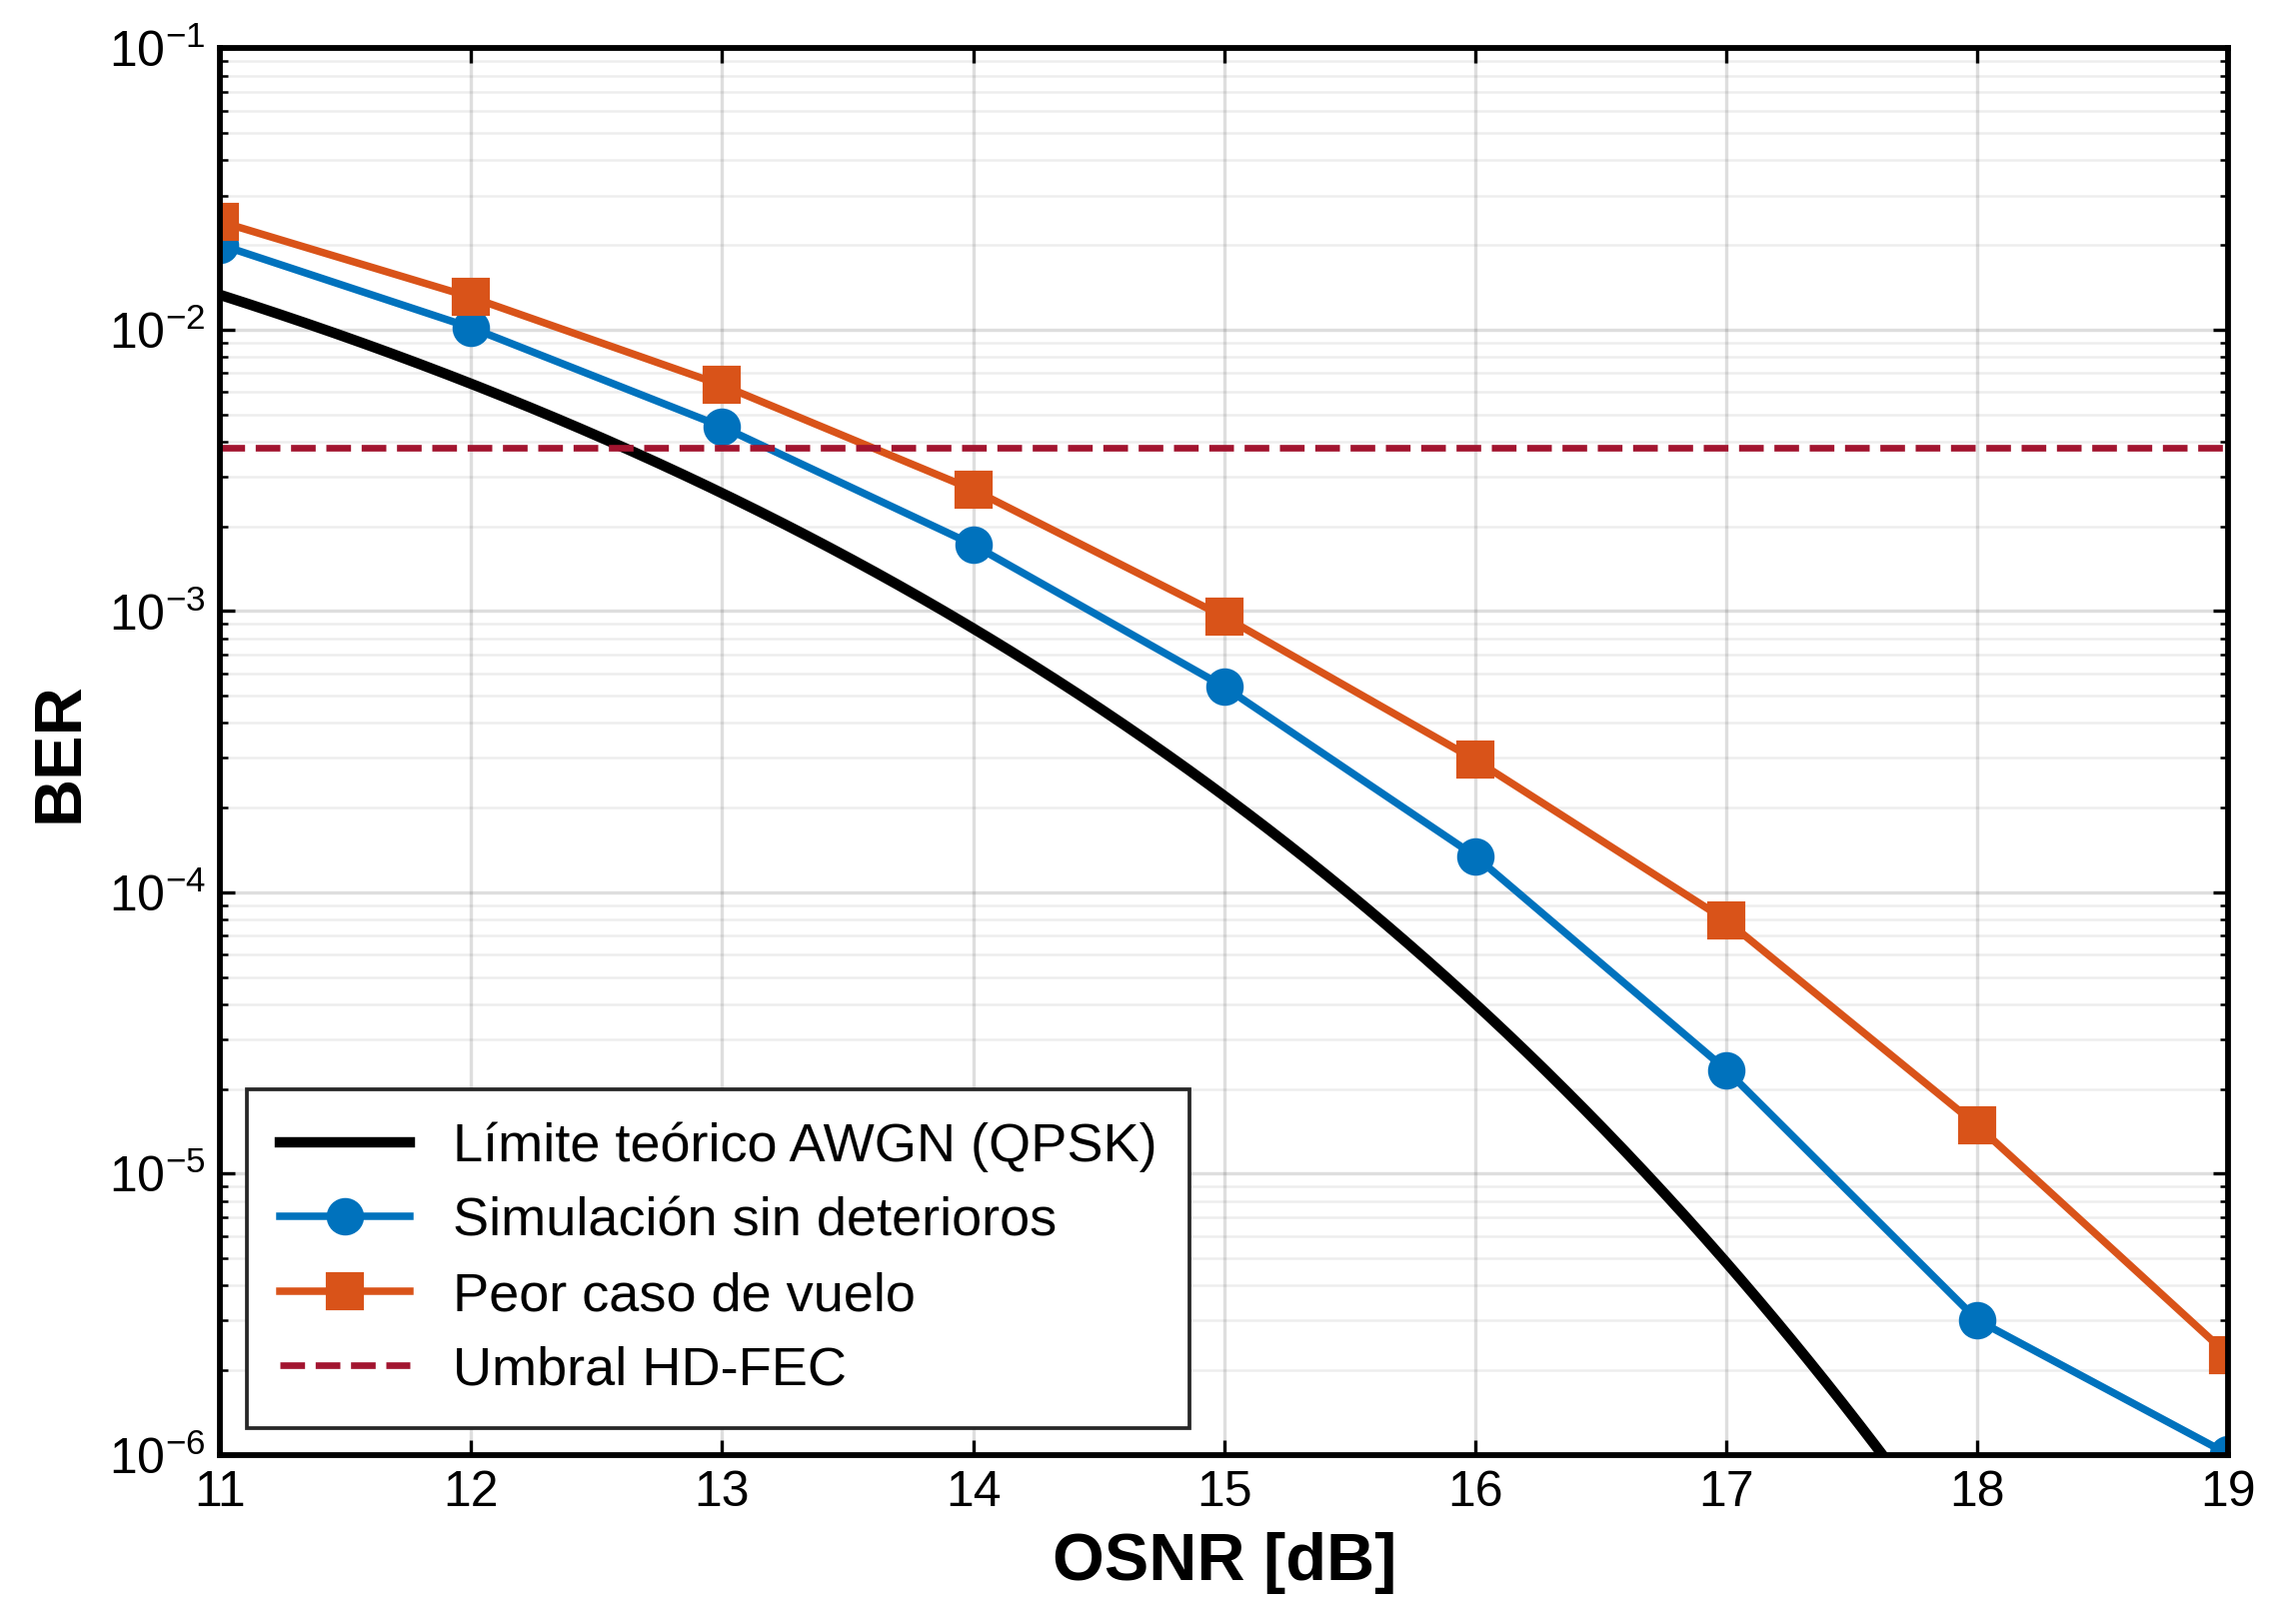
\includegraphics[width=0.85\textwidth]{figuras/ber_vs_osnr.png}
  \caption[Desempe\~no simulado contra el l\'imite te\'orico]{%
    BER contra OSNR. La curva negra es el l\'imite te\'orico AWGN de la
    \cref{eq:ber-qpsk}. La curva azul representa la cadena completa sin
    desbalances y la naranja, el peor caso de vuelo. Las dos separaciones
    horizontales sobre el umbral HD-FEC son la penalidad de implementaci\'on
    del receptor y el costo de los deterioros de vuelo.}
  \label{fig:ber-osnr}
\end{figure}

Como se observa en la \cref{fig:ber-osnr}, en ausencia de deterioros el umbral
HD-FEC se alcanza con una $\OSNR$ de \SI{13.18}{\dB}, frente a los
\SI{12.61}{\dB} del receptor ideal de la \cref{tab:cadena-teorica}. Esa
diferencia representa una penalidad de implementaci\'on de \SI{0.57}{\dB},
atribuible a las limitaciones del receptor y al error residual de los
algoritmos de compensaci\'on del DSP. Al incorporar los deterioros de vuelo de
manera simult\'anea, la OSNR requerida sube a \SI{13.60}{\dB}, es decir
\SI{0.42}{\dB} m\'as. La \cref{tab:umbral} resume los resultados.

\begin{table}[htbp]
  \centering

  \begin{tabular}{llc}
    \toprule
    Configuraci\'on & Penalidad & $\OSNR$ en el umbral \\
    \midrule
    Te\'orico AWGN            & ---                                   & \SI{12.61}{\dB} \\
    Receptor sin deterioros   & $+\SI{0.57}{\dB}$ de implementaci\'on & \SI{13.18}{\dB} \\
    Peor caso de vuelo        & $+\SI{0.42}{\dB}$ de deterioros       & \SI{13.60}{\dB} \\
    \bottomrule
  \end{tabular}
  \caption[Descomposici\'on del umbral operativo]{%
    Penalidad desde el receptor ideal al umbral operativo. La \'ultima fila es
    la que se usa en el balance de potencia.}
  \label{tab:umbral}
\end{table}

De los dos t\'erminos, el mayor es la penalidad de implementaci\'on. Los
deterioros de vuelo con valores de especificaci\'on aportan menos de medio
decibel entre todos.
\section{T\'erminos no contemplados en el balance}
\label{sec:enl-critica}

Se enumeran ciertos aspectos del balance que no se tienen en cuenta, o se simplifican por el alcance del proyecto:
\begin{puntos}
\item{La p\'erdida de apuntamiento es una estimaci\'on:}
En un enlace real el apuntamiento no es un error fijo sino un proceso aleatorio, y es controlado por el Sistema de Control de Actitud (ACS). Sin embargo, para simplicidad se utiliz\'o \SI{5}{\dB} 
de p\'erdidas constantes por este fen\'omeno.

\item{Falta el acoplamiento a fibra monomodo:}
El balance lleva la potencia desde el telescopio de recepci\'on hasta la
entrada del pre-amplificador sin ning\'un t\'ermino intermedio. En realidad, el
haz recibido tiene que acoplarse a una fibra monomodo. En este proceso se tienen dos tipos 
de p\'erdidas. En primer lugar est\'a el desajuste entre el campo de una apertura circular
uniformemente iluminada y el modo gaussiano de la fibra. Por otro lado, se tiene el error de frente de onda residual del
telescopio. Ninguno de estos efectos se tuvo en cuenta debido a la complejidad de sus implementaciones.


\item{No hay margen de sistema asignado:}
El balance se cierra con \SI{3.5}{\dB} entre el umbral operativo y el
l\'imite de saturaci\'on del booster, sin reservar margen para la degradaci\'on
de los componentes a lo largo de la vida \'util. Esto incluye el envejecimiento del l\'aser, la
deriva t\'ermica del punto de polarizaci\'on del modulador y las tolerancias
de fabricaci\'on entre unidades, que una misi\'on real cubre con un margen de
sistema reservado desde el dise\~no.

\end{puntos}
El resultado es que el balance de potencia cierra o no seg\'un las penalidades de estos factores. Un an\'alisis detallado de los subsistemas del sat\'elite es una continuaci\'on natural del proyecto.
\section{Conclusiones}
\label{sec:enl-conclusiones}

El balance de potencia permiti\'o evaluar la viabilidad del enlace LEO--GEO
bajo las condiciones de dise\~no consideradas. A \SI{45000}{\kilo\metre}, los
componentes de la \cref{tab:balance} alcanzan la OSNR necesaria para operar por
debajo del umbral HD-FEC, con un margen de \SI{3.5}{\dB} hasta la saturaci\'on
del booster.

La simulaci\'on completa cuantific\'o una penalidad de implementaci\'on de
\SI{0.57}{\dB} respecto del l\'imite te\'orico AWGN, a la que se suman
\SI{0.42}{\dB} asociados a los deterioros de vuelo. El requisito de OSNR para
el dimensionamiento del enlace queda entonces en \SI{13.60}{\dB}.

El balance no contempla las p\'erdidas de acoplamiento a fibra monomodo ni
reserva un margen de sistema para degradaciones e incertidumbres adicionales.
Las p\'erdidas por apuntamiento, adem\'as, se aproximaron con una penalidad
constante de \SI{5}{\dB}. La viabilidad del enlace queda condicionada a que
estos efectos se mantengan dentro del margen disponible. Por \'ultimo, el
an\'alisis se hizo cerca de la separaci\'on m\'axima entre los sat\'elites, de
modo que operar a distancias menores deja m\'as margen de potencia.

% !TeX root = ../main.tex
\chapter{Tolerancia a las degradaciones del canal}
\label{cap:tolerancias}

\section{Introducci\'on}
\label{sec:tol-intro}

En este cap\'itulo se eval\'uan los l\'imites de operaci\'on del receptor
frente a cada una de las degradaciones consideradas. Para cada deterioro se
barre la variable que lo controla, aumentando su magnitud hasta que el
receptor deja de cumplir el requisito de BER, y se identifica el mecanismo
que produce la falla.

Se tiene dos objetivos. Por un lado, entender qu\'e limita el desempe\~no en
cada caso. Por otro, cuantificar el margen que queda entre el l\'imite medido
y el valor que el enlace realmente impone, calculado en el \cref{cap:canal}.
Los resultados se re\'unen en una tabla al final del cap\'itulo.

\section{Metodolog\'ia}
\label{sec:tol-metodologia}

\paragraph{M\'etrica de evaluaci\'on:}
Para evaluar la tolerancia del receptor se utiliza la magnitud del vector de
error, EVM, tomada siempre sobre la polarizaci\'on de peor desempe\~no y no
sobre el promedio de las dos. Se toma la peor porque algunas fallas del
receptor afectan a una sola polarizaci\'on, y promediarlas disimular\'ia el colapso.

\paragraph{Estimaci\'on de la penalidad de OSNR:}
La penalidad asociada a un deterioro es el incremento de OSNR necesario para
mantener el desempe\~no en el umbral HD-FEC. Determinarla de forma directa
obligar\'ia a correr un barrido de OSNR completo en cada punto, con un costo
de simulaci\'on muy alto. En su lugar se la estima a partir del EVM,
aprovechando que en QPSK con ruido gaussiano aditivo vale
$\EVM^{2} = 1/\mathrm{SNR}$, con el EVM normalizado al valor eficaz de la
constelaci\'on de referencia.

La conversi\'on tiene dos pasos. Primero se separa en cuadratura lo que
aporta el deterioro de lo que aporta el ruido \'optico, que ya estaba en el
punto limpio. Despu\'es se convierte esa fracci\'on del presupuesto de error
en decibeles.
\begin{equation}
  \EVM_{\mathrm{imp}}^{2} = \EVM_{\mathrm{med}}^{2} - \EVM_{\mathrm{limpio}}^{2},
  \qquad
  \mathcal{P}\,[\si{\dB}] = -10\log_{10}\!
  \left[1 - \left(\frac{\EVM_{\mathrm{imp}}}{\EVM_{\mathrm{th}}}\right)^{2}\right],
  \label{eq:tol-penalidad}
\end{equation}
con $\EVM_{\mathrm{th}} = \SI{37.46}{\percent}$ el EVM que corresponde al
umbral HD-FEC.

\section{Offset de frecuencia Doppler}
\label{sec:tol-doppler}

El desplazamiento Doppler introduce una diferencia de frecuencia entre la
portadora \'optica recibida y el oscilador local del receptor, que el DSP
tiene que estimar y compensar. En la \cref{eq:requisito-captura} se
estableci\'o un requisito de captura de \SI{\pm 6.0}{\giga\hertz} para el
enlace LEO--GEO. En esta secci\'on se eval\'ua en simulaci\'on el rango de
frecuencias que el receptor puede compensar, y se verifica su cumplimiento
para las tres tasas de s\'imbolo consideradas.

\begin{figure}[H]
  \centering
  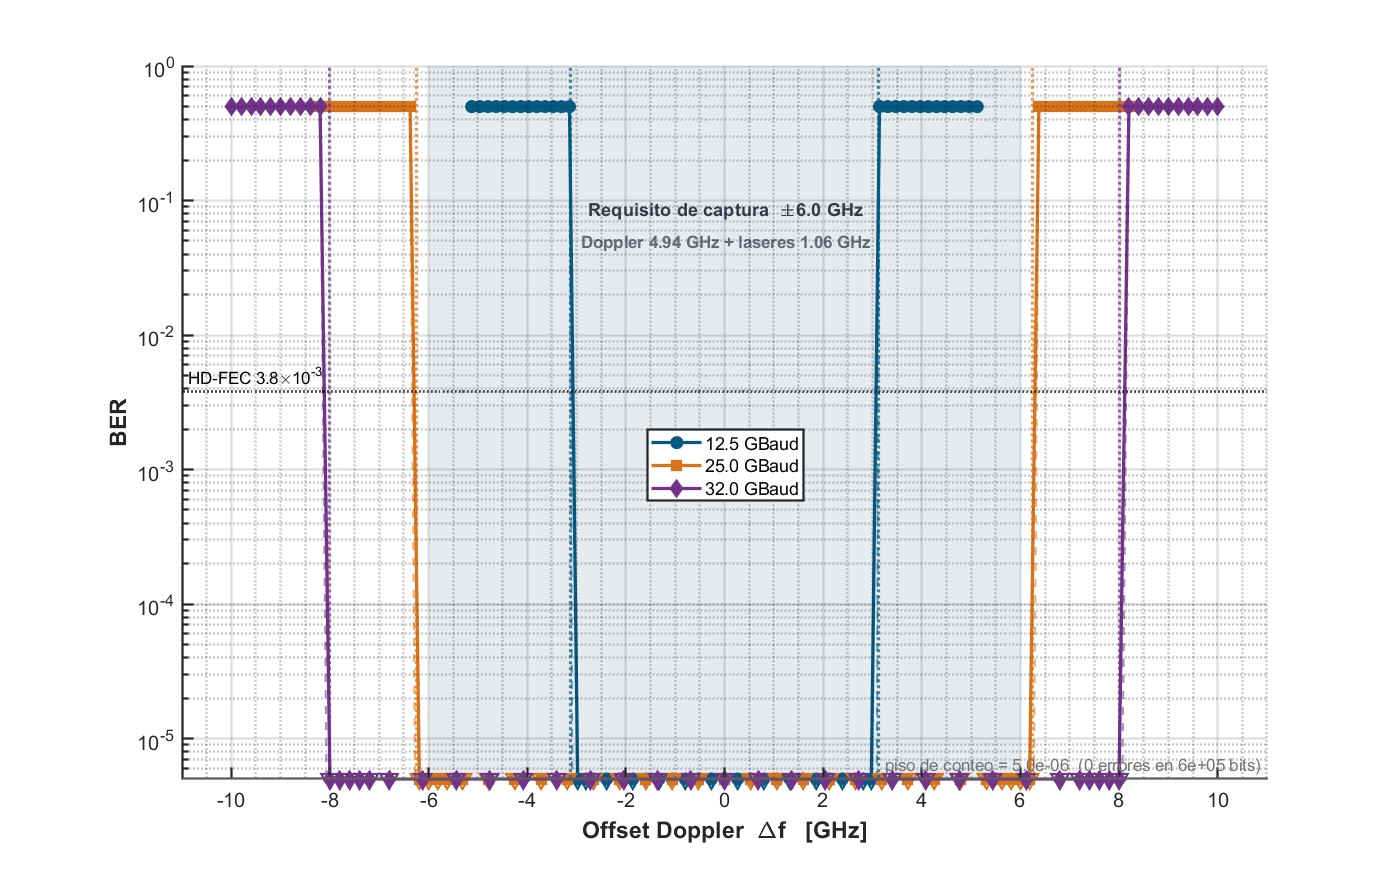
\includegraphics[width=0.92\textwidth]{figuras/EfectoDopplerFiguraFinalSimulacion.jpg}
  \caption[Tolerancia al offset Doppler en simulaci\'on]{%
    BER contra offset Doppler para las tres tasas de s\'imbolo para una OSNR
    fija, en simulaci\'on. La franja sombreada es el requisito de captura del
    enlace, \SI{\pm 6.0}{\giga\hertz}. La l\'inea de trazos es el umbral
    HD-FEC.}
  \label{fig:tol-doppler-sim}
\end{figure}

La \cref{fig:tol-doppler-sim} muestra que la BER se mantiene
aproximadamente constante dentro de un intervalo de frecuencias, a partir del
cual sube de forma abrupta hasta valores cercanos a \num{0.5}, sin
degradaci\'on gradual.

Los l\'imites de captura obtenidos son de \SI{\pm 3.1}{\giga\hertz} a
\SI{12.5}{\giga\baud}, \SI{\pm 6.25}{\giga\hertz} a \SI{25}{\giga\baud} y
\SI{\pm 8.0}{\giga\hertz} a \SI{32}{\giga\baud}, es decir $\Rs/4$ en las
tres. El mecanismo est\'a explicado en la \cref{sec:dsp-frec-limite}. El
estimador trabaja sobre la se\~nal elevada a la cuarta potencia, de modo que
el offset aparece como un tono en $4\Df$. La se\~nal est\'a muestreada a dos
muestras por s\'imbolo, as\'i que $F_s = 2\Rs$ y la frecuencia de Nyquist es
$F_s/2 = \Rs$. La igualdad $4\Df = \Rs$ se alcanza en $\Df = \Rs/4$, y por
encima de ese valor el tono se pliega y el estimador deja de identificar
correctamente el offset.

El mecanismo se puede observar de forma directa mirando qu\'e frecuencia
entrega el estimador. La \cref{fig:tol-frecuencia-estimada} compara la
estimaci\'on contra el offset realmente aplicado, para las mismas tres tasas
de s\'imbolo.

\begin{figure}[H]
  \centering
  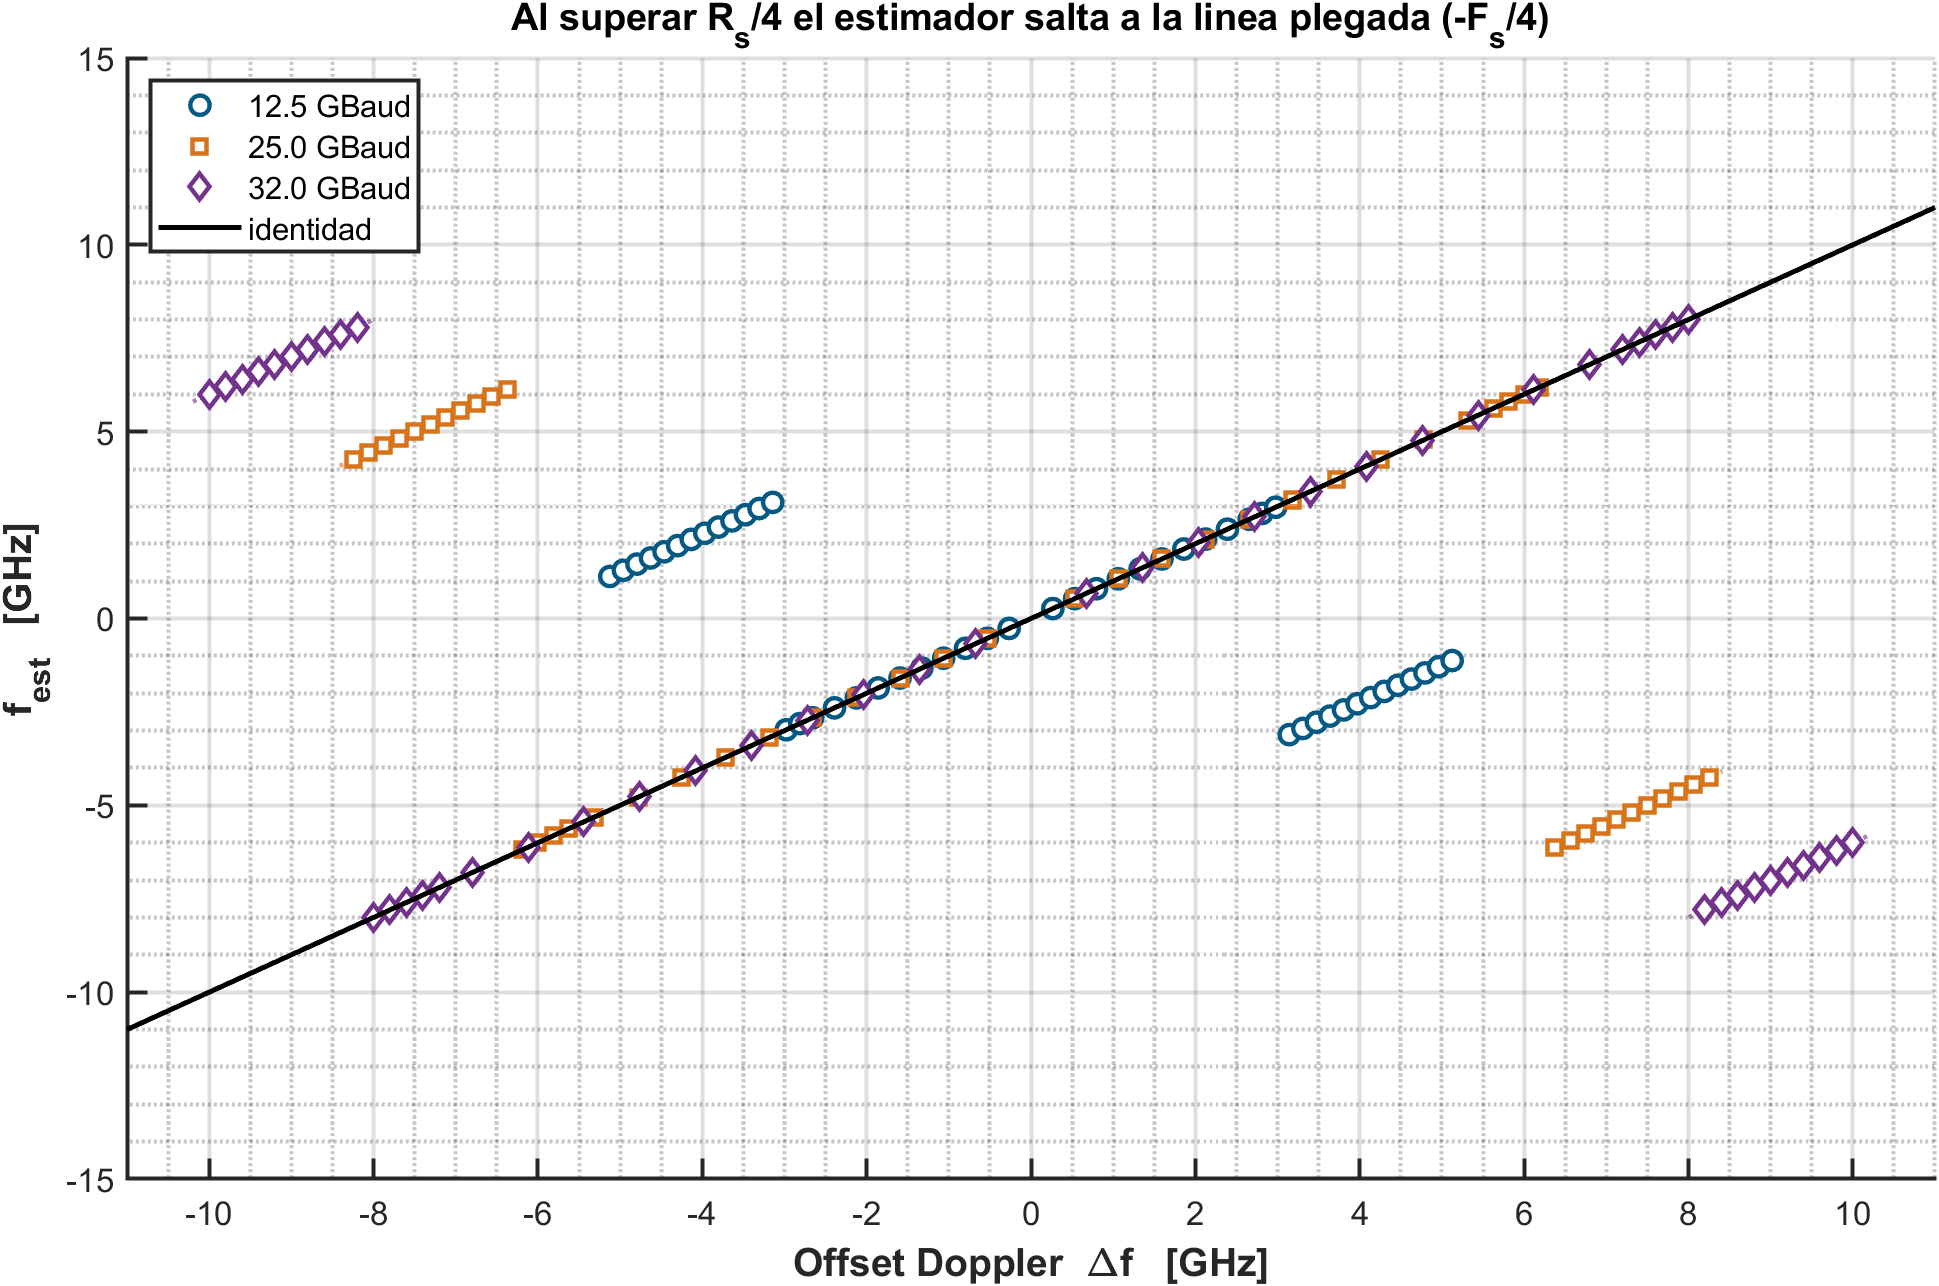
\includegraphics[width=0.92\textwidth]{figuras/tol_frecuencia_estimada.png}
  \caption[Frecuencia estimada contra offset aplicado]{%
    Frecuencia estimada por el bloque de recuperaci\'on en funci\'on del offset
    aplicado, para las tres tasas de s\'imbolo. La recta negra es la
    identidad. Mientras el tono cae dentro de la banda de Nyquist la
    estimaci\'on la sigue. Pasado $\Rs/4$ el tono se pliega y la estimaci\'on
    salta a una segunda recta, paralela a la primera y desplazada en
    $\Rs/2$.}
  \label{fig:tol-frecuencia-estimada}
\end{figure}

Mientras el tono cae dentro de la banda, la estimaci\'on sigue la identidad
en las tres tasas. Pasado $\Rs/4$ no se vuelve err\'atica sino que salta a un
valor determinado,
\begin{equation}
  f_{\mathrm{est}} = \Df - \frac{\Rs}{2},
  \label{eq:tol-plegado}
\end{equation}
que es la posici\'on del tono plegado. El salto escala con la tasa de
s\'imbolo, de \SI{6.25}{\giga\hertz} a \SI{12.5}{\giga\baud} a
\SI{16}{\giga\hertz} a \SI{32}{\giga\baud}, lo que confirma que el l\'imite
de captura lo fija d\'onde cae el tono dentro de la banda de Nyquist.

\begin{table}[htbp]
  \centering

  \begin{tabular}{lccc}
    \toprule
     $\Rs$ & $\Rs/4$ & Simulaci\'on & Margen \\
    \midrule
    \SI{12.5}{\giga\baud} & \SI{3.125}{\giga\hertz} & \SI{\pm 3.1}{\giga\hertz}  & \SI{-2.9}{\giga\hertz}  \\
    \SI{25}{\giga\baud}   & \SI{6.25}{\giga\hertz}  & \SI{\pm 6.25}{\giga\hertz} & \SI{+0.25}{\giga\hertz} \\
    \SI{32}{\giga\baud}   & \SI{8.0}{\giga\hertz}   & \SI{\pm 8.0}{\giga\hertz}  & \SI{+2.0}{\giga\hertz}  \\
    \bottomrule
  \end{tabular}
  \caption[Ventana de captura de Doppler]{%
    Ventana de captura medida en simulaci\'on contra el l\'imite te\'orico
    $\Rs/4$. La \'ultima columna es la diferencia con el requisito de captura
    del enlace, \SI{\pm 6.0}{\giga\hertz}.}
  \label{tab:tol-doppler}
\end{table}

La tolerancia al offset crece con la tasa de s\'imbolo. A
\SI{12.5}{\giga\baud} el rango de captura no alcanza para cubrir el requisito
de \SI{\pm 6.0}{\giga\hertz}. A \SI{25}{\giga\baud} el requisito se cumple,
aunque con un margen reducido de \SI{0.25}{\giga\hertz}. A
\SI{32}{\giga\baud} el margen es de \SI{2.0}{\giga\hertz}, de modo que el
receptor cumple con holgura.

\subsection{Dependencia con la relaci\'on se\~nal-ruido}
\label{sec:tol-doppler-osnr}

Para evaluar la influencia del ruido \'optico sobre el rango de captura, se
repiti\'o el barrido de offset a \SI{32}{\giga\baud} para doce valores de
OSNR entre \SI{10}{\dB} y \SI{21}{\dB}.

\begin{figure}[H]
  \centering
  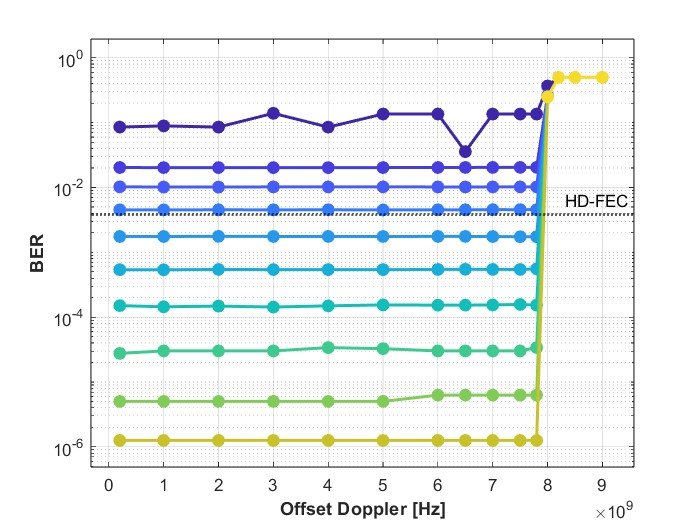
\includegraphics[width=0.92\textwidth]{figuras/tol_doppler_osnr.jpg}
  \caption[Offset Doppler contra la familia de OSNR]{%
    BER contra offset Doppler para doce valores de OSNR. El color denota una
    OSNR en pasos de \SI{1}{\dB}, de azul oscuro en \SI{10}{\dB} a amarillo
    en \SI{21}{\dB}. Las curvas se desplazan verticalmente con la OSNR pero
    quiebran todas en el mismo punto.}
  \label{fig:tol-doppler-osnr}
\end{figure}

Como se observa en la \cref{fig:tol-doppler-osnr}, para OSNR entre
\SI{13}{\dB} y \SI{21}{\dB} el receptor funciona hasta
\SI{7.8}{\giga\hertz} y colapsa en \SI{8.0}{\giga\hertz}. El quiebre no se
desplaza con la OSNR y queda en $\Rs/4$ en todos los casos, que es el mismo
plegado de la \cref{fig:tol-frecuencia-estimada}. Al tratarse de un efecto de
muestreo, el nivel de ruido no lo corre. Por debajo de \SI{13}{\dB} se
observan degradaciones adicionales, posiblemente asociadas a dificultades del
lazo de recuperaci\'on de fase.

\section{Tasa de chirp Doppler}
\label{sec:tol-chirp}

El desplazamiento Doppler no es constante a lo largo del pase, porque la
velocidad radial relativa entre los sat\'elites var\'ia. Eso produce una
deriva temporal de la frecuencia recibida, cuya tasa m\'axima se estim\'o en
\SI{6.55}{\mega\hertz\per\second} para las condiciones de vuelo
consideradas. En esta secci\'on se mide cu\'anta deriva tolera el receptor.

\begin{figure}[H]
  \centering
  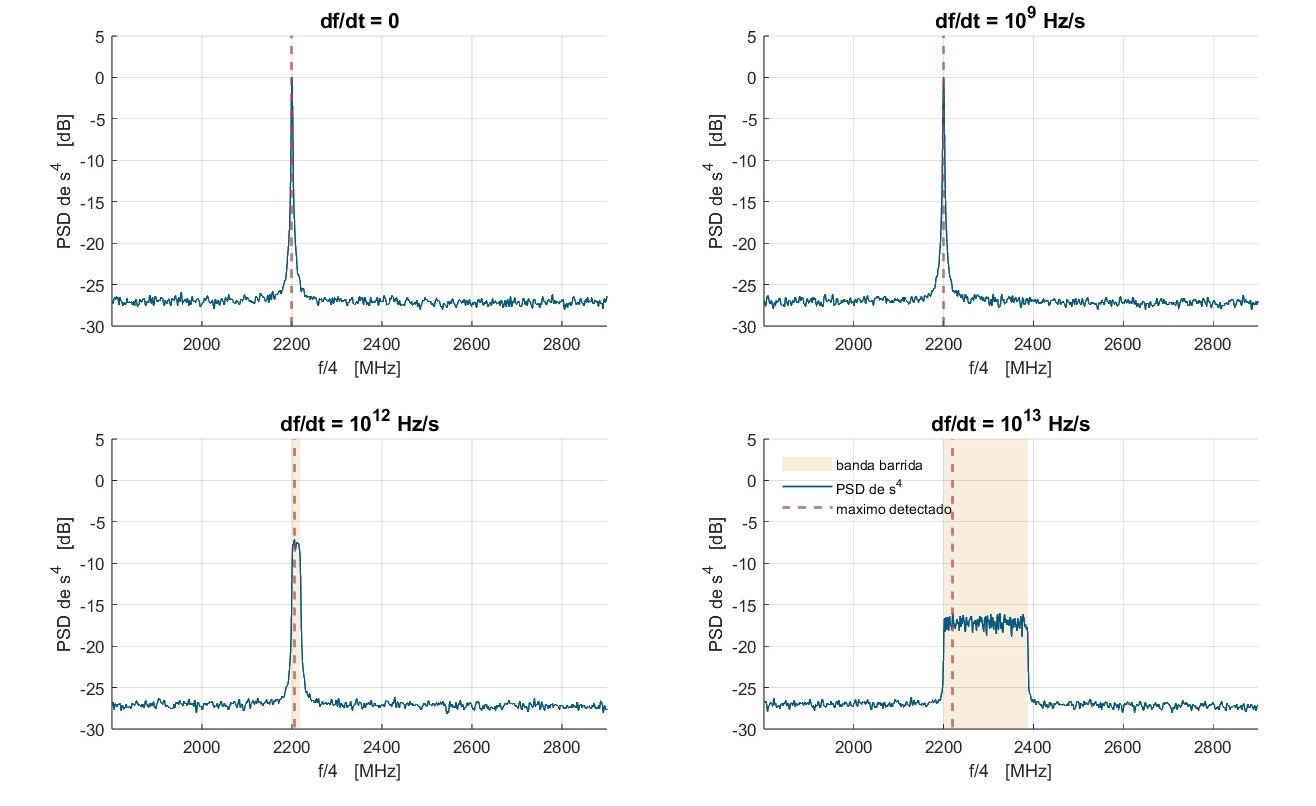
\includegraphics[width=0.92\textwidth]{figuras/EfectoChirp.jpg}
  \caption[Efecto del chirp sobre el espectro de la cuarta potencia]{%
    Densidad espectral de la se\~nal elevada a la cuarta para cuatro tasas de
    chirp, con una ventana de \SI{18.75}{\micro\second} y un offset de
    \SI{2200}{\mega\hertz}. La franja marca la banda barrida durante la
    ventana y la l\'inea de trazos, el m\'aximo que detecta el estimador.}
  \label{fig:tol-efecto-chirp}
\end{figure}

La \cref{fig:tol-efecto-chirp} muestra el efecto del chirp sobre el estimador
de frecuencia. A diferencia de un offset constante, una frecuencia que var\'ia
linealmente con el tiempo ensancha la componente espectral que el estimador
utiliza, porque durante una ventana de duraci\'on $T$ el offset recorre
$\dot f\,T$. Para una tasa de \SI{1e13}{\hertz\per\second} y una ventana de
\SI{18.75}{\micro\second} son \SI{187.5}{\mega\hertz}, y el tono deja de ser
una l\'inea para convertirse en una meseta de \num{2200} a
\SI{2390}{\mega\hertz}. La altura del pico cae en proporci\'on inversa al
ensanchamiento, de \SI{0}{\dB} a \SI{-17}{\dB}, y el estimador se queda con
uno de los m\'aximos dentro de ese rango.

El estimador entrega un \'unico valor de frecuencia para toda la secuencia
procesada, de modo que no puede seguir su variaci\'on temporal. Despu\'es de
la compensaci\'on queda un offset residual que var\'ia a lo largo del
registro, como muestra la \cref{fig:tol-rampa-frecuencia}.

\begin{figure}[H]
  \centering
  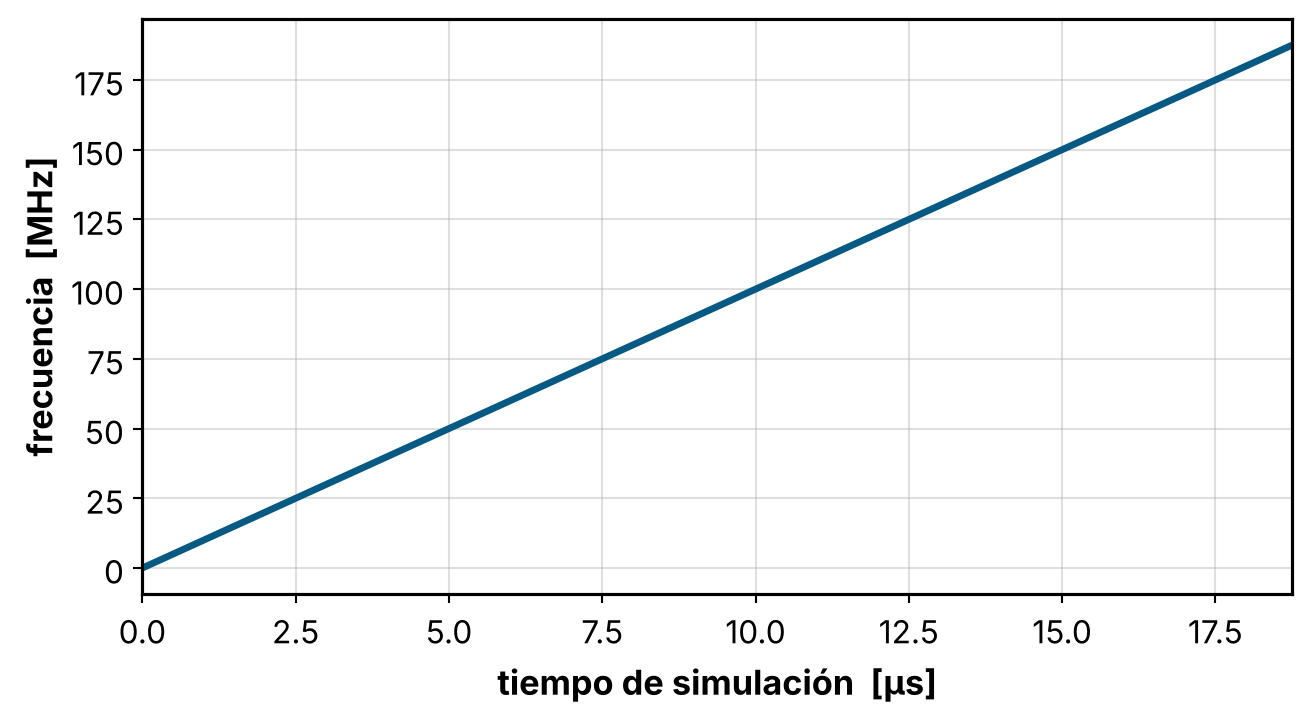
\includegraphics[width=0.78\textwidth]{figuras/rampa_frecuencia_chirp.png}
  \caption[Rampa de frecuencia dejada por el chirp]{%
    Frecuencia instant\'anea a lo largo del registro para un offset inicial
    nulo y una tasa de chirp de \SI{1e13}{\hertz\per\second}.}
  \label{fig:tol-rampa-frecuencia}
\end{figure}

El lazo de recuperaci\'on de fase es de segundo orden, as\'i que ante una
rampa de frecuencia queda con un error de fase estacionario. Ese residuo,
sumado al ruido de fase que aportan el l\'aser transmisor y el oscilador
local, es lo que el lazo tiene que absorber mientras el ecualizador converge.

\begin{figure}[H]
  \centering
  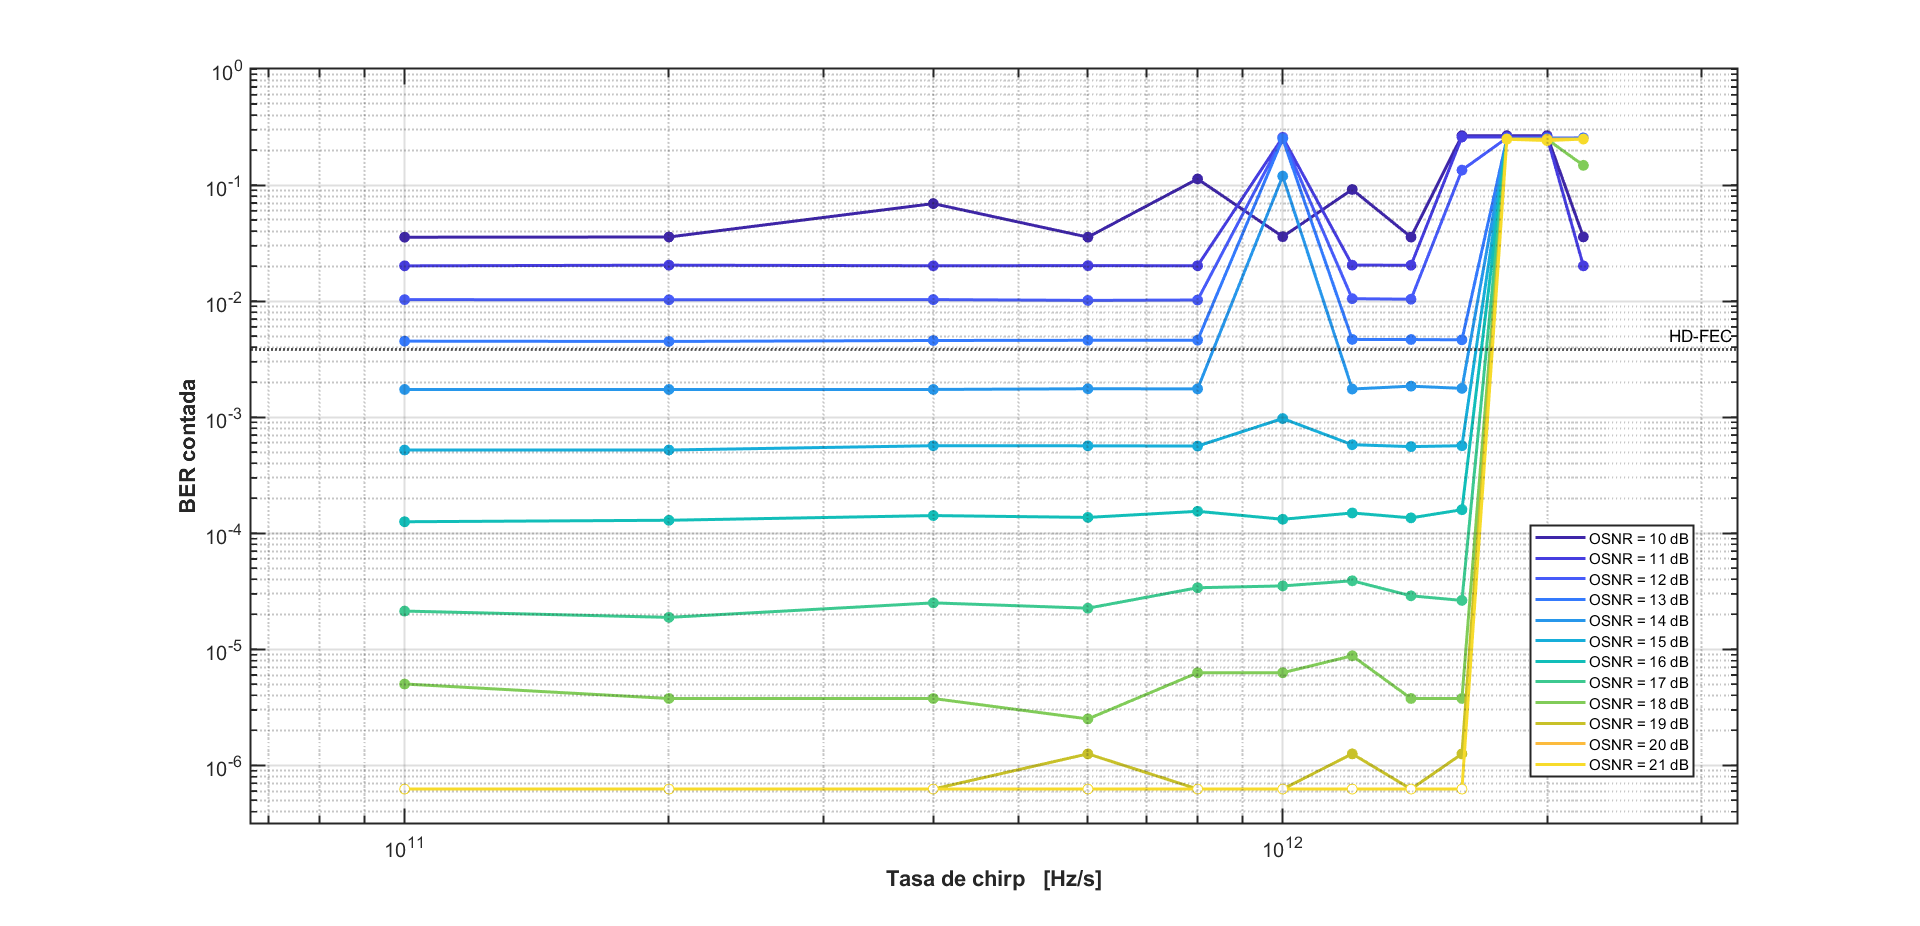
\includegraphics[width=0.92\textwidth]{figuras/tol_chirp_osnr.png}
  \caption[Tolerancia a la tasa de chirp]{%
    BER contra tasa de chirp Doppler para doce valores de OSNR. El color determina la OSNR en pasos de \SI{1}{\dB}, de azul
    oscuro en \SI{10}{\dB} a amarillo en \SI{21}{\dB}. Los c\'irculos huecos
    son puntos sin ning\'un error, dibujados en el piso de conteo. De
    \SI{14}{\dB} en adelante las curvas son planas hasta
    \SI{1.6e12}{\hertz\per\second} y suben hasta \num{0.25} antes de
    \SI{1.8e12}{\hertz\per\second}.}
  \label{fig:tol-chirp}
\end{figure}

La \cref{fig:tol-chirp} barre doce tasas entre \num{1e11} y
\SI{2.2e12}{\hertz\per\second} para doce valores de OSNR. De \SI{14}{\dB} en
adelante la BER se mantiene aproximadamente constante hasta
\SI{1.6e12}{\hertz\per\second} y cruza el umbral HD-FEC entre \num{1.6e12} y
\SI{1.8e12}{\hertz\per\second}, en el mismo intervalo para todas.

El l\'imite no se desplaza con la OSNR. El ruido \'optico no corre el umbral,
pero vuelve a las curvas menos regulares, con fallas aisladas que aparecen en
un punto y desaparecen en el siguiente, como la de
\SI{1e12}{\hertz\per\second} entre \num{11} y \SI{14}{\dB}. Por debajo de
\SI{13}{\dB} las curvas ya arrancan por encima del umbral.

Los resultados sugieren que la falla se asocia a la incapacidad del lazo de
recuperaci\'on de fase para compensar el residuo que deja la variaci\'on
temporal del offset. El quiebre est\'a en \SI{1.8e12}{\hertz\per\second},
m\'as de cinco \'ordenes de magnitud por encima de los
\SI{6.55}{\mega\hertz\per\second} que impone el peor instante del pase, de
modo que el chirp Doppler no representa una limitaci\'on para el enlace.

\section{Rotaci\'on del estado de polarizaci\'on}
\label{sec:tol-sop}

La variaci\'on de la geometr\'ia del enlace LEO--GEO produce una rotaci\'on
din\'amica del estado de polarizaci\'on de la se\~nal recibida, que el
ecualizador MIMO tiene que seguir y compensar. En esta secci\'on se eval\'ua
la capacidad de seguimiento del receptor barriendo la velocidad angular de
rotaci\'on $\dot\theta$ para distintas condiciones de OSNR.

\begin{figure}[H]
  \centering
  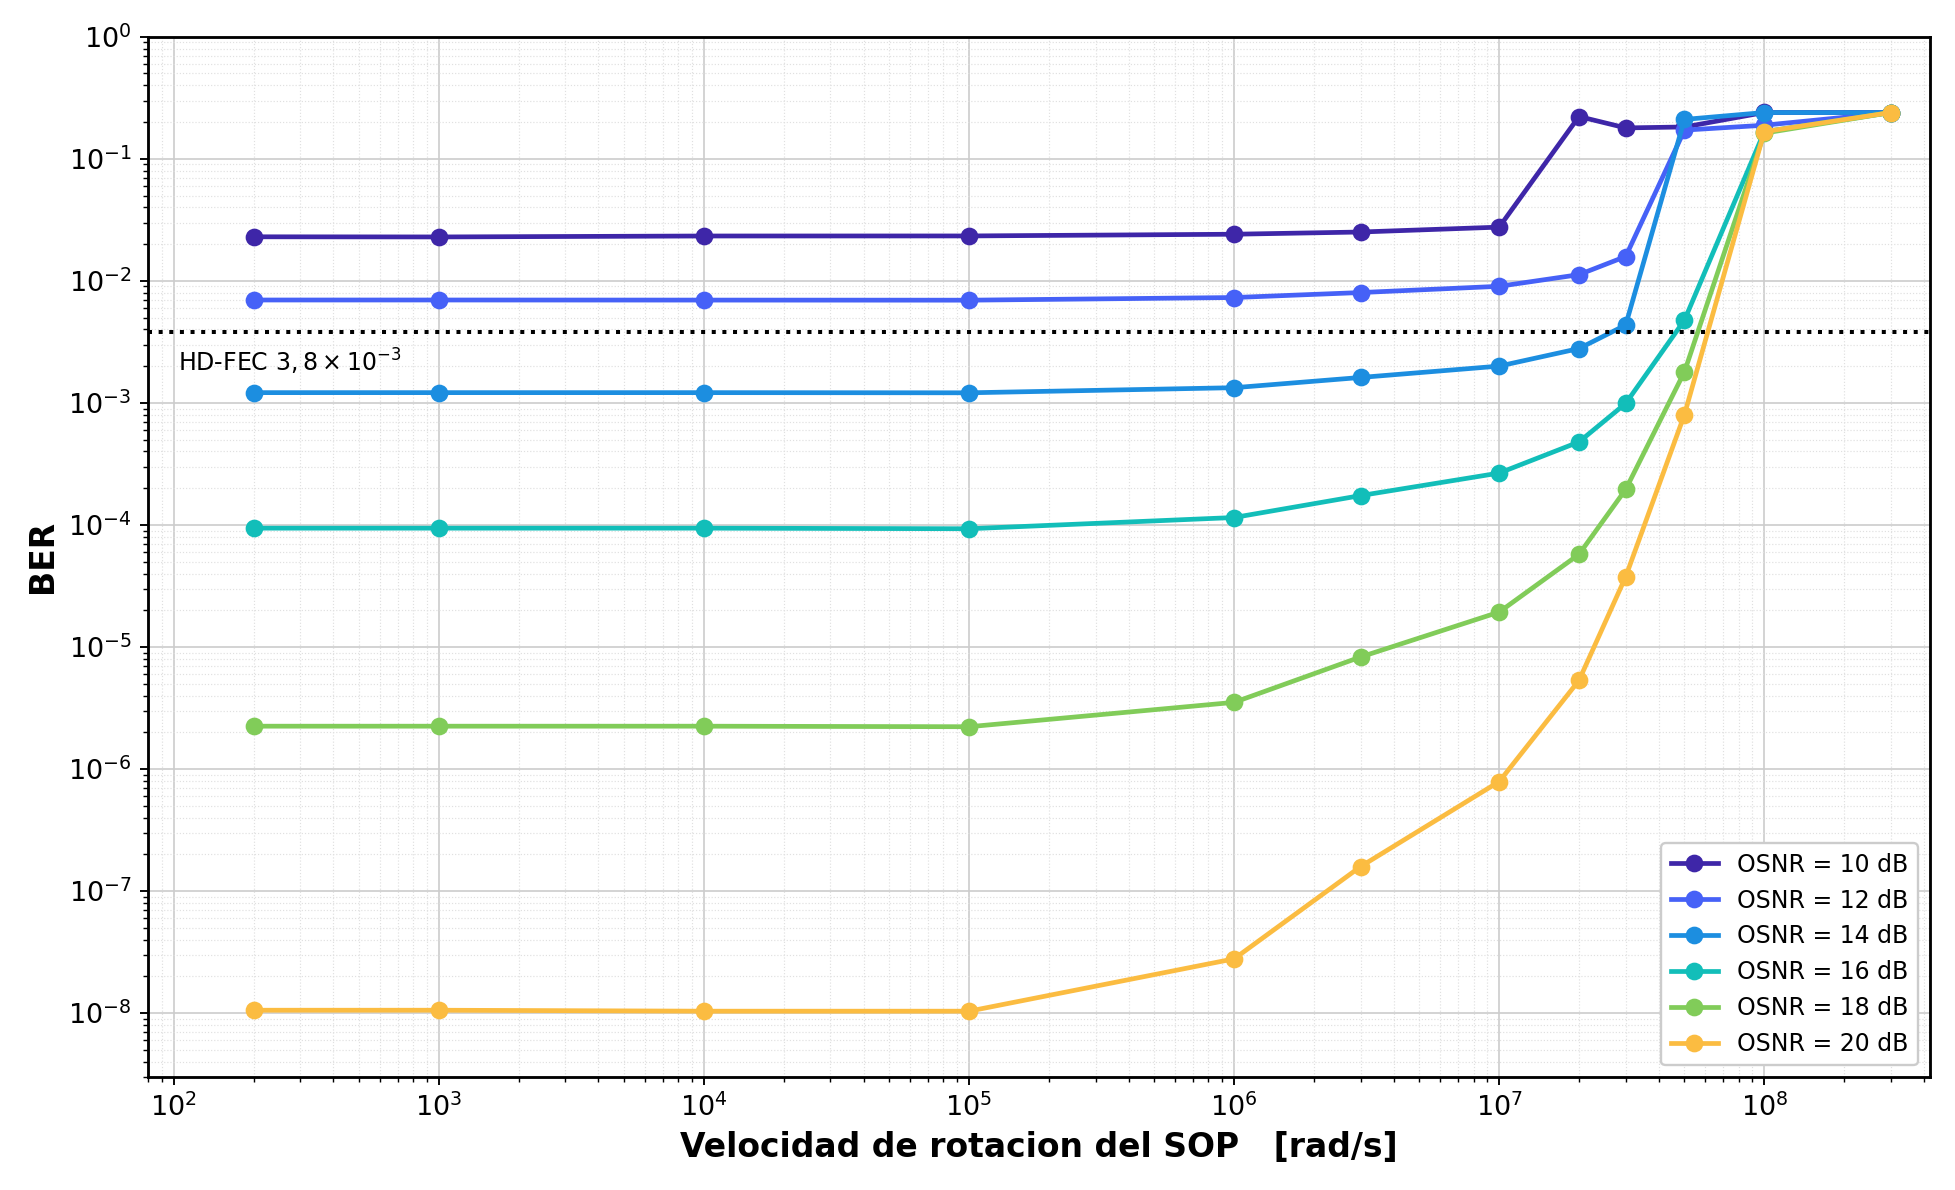
\includegraphics[width=0.92\textwidth]{figuras/SOPOSNR_BER.png}
  \caption[Tolerancia a la rotaci\'on del estado de polarizaci\'on]{%
    BER contra velocidad de rotaci\'on del estado de polarizaci\'on para una
    familia de OSNR. La degradaci\'on empieza a notarse en
    \SI{1e6}{\radian\per\second}, con la primera degradaci\'on pr\'acticamente en el mismo
    lugar para todas las OSNR.}
  \label{fig:tol-sop}
\end{figure}

La capacidad de seguimiento del ecualizador depende de su paso de
adaptaci\'on $\mu$. Un paso mayor actualiza los coeficientes m\'as r\'apido y
reduce el retardo frente a las variaciones del estado de polarizaci\'on.
Tomando una constante de tiempo de adaptaci\'on proporcional a
$1/(\mu\Rs)$~\cite{haykin2014}, el error angular de seguimiento queda, de
forma aproximada,
\begin{equation}
  \theta_{\mathrm{lag}} = \frac{\dot\theta}{\mu \Rs}.
  \label{eq:tol-lag}
\end{equation}
Esta relaci\'on sugiere que, para un error angular m\'aximo tolerable, la
velocidad de rotaci\'on que el ecualizador puede compensar crece en
proporci\'on directa con $\mu$. La \cref{fig:tol-sop-mu} barre doce pasos de
adaptaci\'on y muestra hasta d\'onde vale esa proporcionalidad.

\begin{figure}[H]
  \centering
  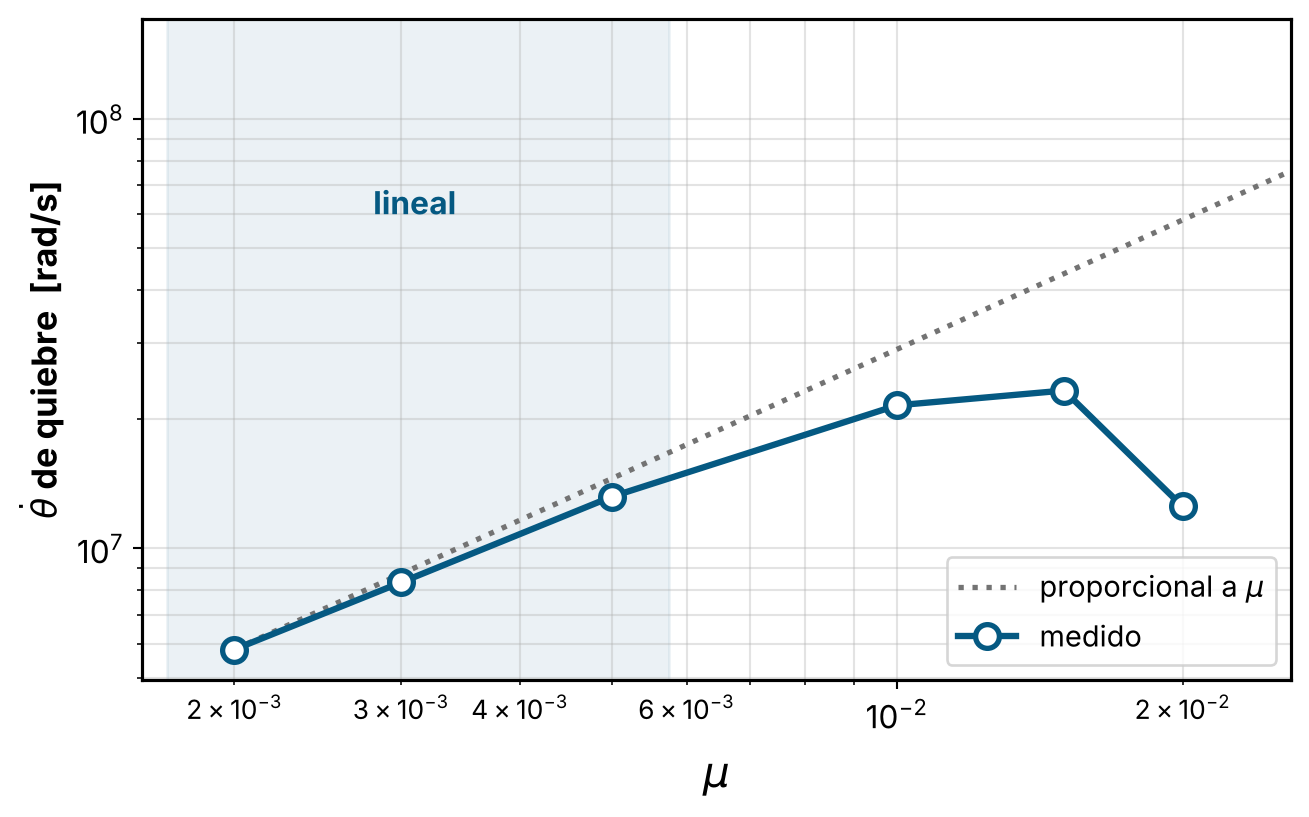
\includegraphics[width=0.82\textwidth]{figuras/tol_quiebre_vs_mu.png}
  \caption[Velocidad de quiebre contra el paso de adaptaci\'on]{%
    Velocidad de rotaci\'on a la que el EVM cruza el umbral HD-FEC, contra el
    paso de adaptaci\'on del ecualizador. La franja marca el tramo en que la
    proporcionalidad con $\mu$ se cumple.}
  \label{fig:tol-sop-mu}
\end{figure}

La proporcionalidad se cumple para los tres pasos m\'as chicos. En
$\mu = \num{0.01}$, que es el valor nominal, el quiebre medido ya se aparta
de la recta, y para valores mayores la tolerancia alcanza un m\'aximo y
despu\'es disminuye.

El comportamiento responde a dos efectos contrapuestos. Un paso mayor permite
seguir variaciones m\'as r\'apidas, pero tambi\'en aumenta el error residual
asociado al ruido de gradiente del ecualizador. El EVM en ausencia de
rotaci\'on sube de \SI{34.4}{\percent} en $\mu = \num{0.002}$ a
\SI{36.6}{\percent} en \num{0.02}, lo que reduce el margen disponible hasta
el umbral HD-FEC. Los dos efectos se compensan alrededor de
$\mu = \num{0.015}$, y por encima de \num{0.025} el receptor deja de cumplir
el requisito de BER incluso con el estado de polarizaci\'on quieto.

Para el paso nominal $\mu = \num{0.01}$ el receptor tolera velocidades de
hasta \SI{2.15e7}{\radian\per\second}, m\'as de diez \'ordenes de magnitud
por encima de los \SI{1e-3}{\radian\per\second} que impone la geometr\'ia del
pase. El estado de polarizaci\'on, por lo tanto, no representa una
limitaci\'on para el enlace.

El modelo de canal incorpora, adem\'as de la deriva geom\'etrica, el jitter
mec\'anico que introduce el control de actitud de la plataforma. Quedan fuera
las variaciones de polarizaci\'on que originan las perturbaciones
mec\'anicas y t\'ermicas sobre los tramos de fibra del transmisor y del
receptor. Dado el margen de diez \'ordenes de magnitud, esos efectos no
cambian la conclusi\'on, pero una implementaci\'on real tiene que
caracterizarlos.

\section{Ruido del l\'aser}
\label{sec:tol-laser}

El ruido de fase del l\'aser transmisor y del oscilador local introduce
fluctuaciones aleatorias en la fase de la se\~nal detectada, que el lazo de
recuperaci\'on de fase tiene que compensar. El par\'ametro barrido en esta
secci\'on es el ancho de l\'inea por l\'aser, $\dnu$. Suponiendo fuentes
independientes con espectro lorentziano, el ancho de l\'inea efectivo del
batido es la suma de los dos.

\subsection{Dependencia con la relaci\'on se\~nal-ruido}
\label{sec:tol-laser-osnr}

\begin{figure}[H]
  \centering
  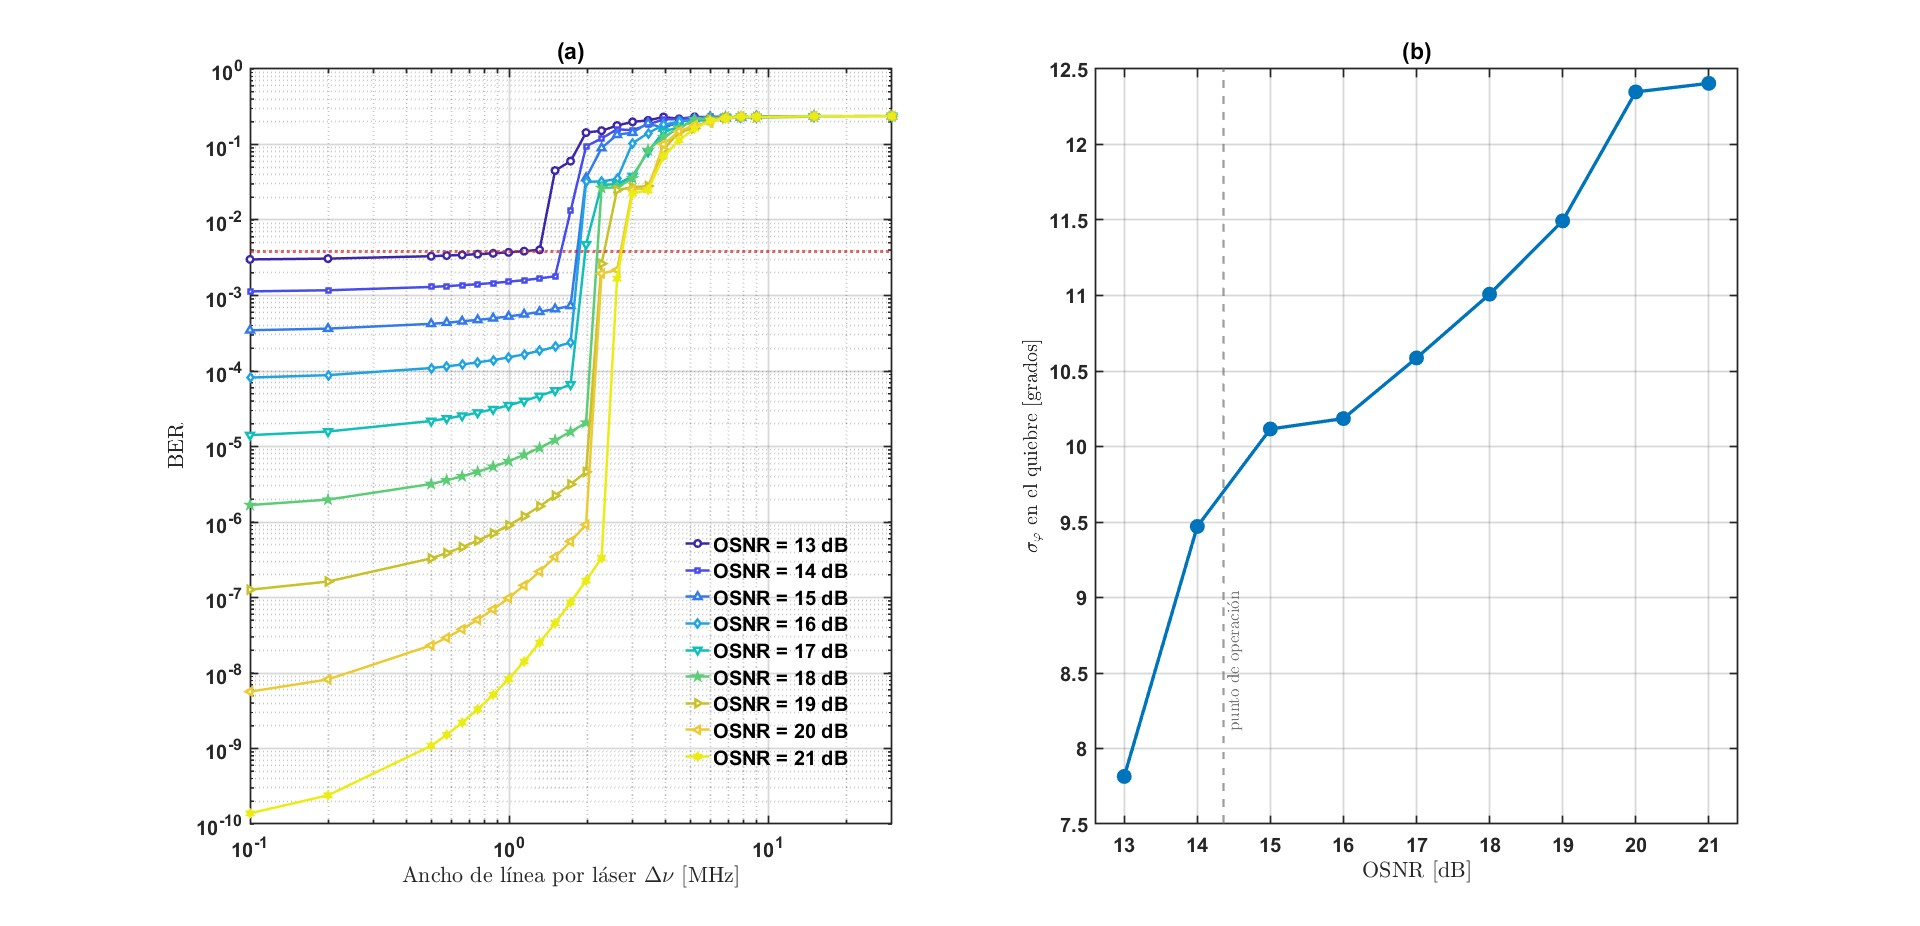
\includegraphics[width=0.98\textwidth]{figuras/TolAnchodeLineaFamiliaOSNR.jpg}
   \caption[Tolerancia al ancho de l\'inea contra OSNR]{%
    (a) BER contra ancho de l\'inea por l\'aser, para una familia de nueve
    valores de OSNR, con $g_1 = \num{0.02}$. El color determina la OSNR en
    pasos de \SI{1}{\dB}, de azul oscuro en \SI{13}{\dB} a amarillo en
    \SI{21}{\dB}. (b) Desviaci\'on est\'andar del error de fase residual,
    evaluada en el quiebre de cada curva. La BER se obtiene del EVM con
    $\mathrm{BER} = Q(1/\EVM)$, que es la misma conversi\'on que define el
    umbral de la \cref{sec:tol-metodologia}.}
  \label{fig:tol-linewidth}
\end{figure}

Como se observa en la \cref{fig:tol-linewidth}a, el aumento del ancho de
l\'inea degrada el desempe\~no de forma gradual. La BER sube de manera
continua y cada curva cruza el umbral en un punto propio. Ese punto mejora
con la OSNR, de \SI{1.6}{\mega\hertz} por l\'aser en \SI{14}{\dB} a
\SI{2.7}{\mega\hertz} en \SI{21}{\dB}.

El panel (b) muestra que la desviaci\'on del error de fase en el quiebre
tampoco es constante. Crece un \SI{59}{\percent} entre \SI{13}{\dB} y
\SI{21}{\dB}. Con menos ASE queda m\'as EVM disponible antes del umbral, de
modo que el lazo tolera excursiones de fase mayores. El l\'imite de
tolerancia al ruido de fase depende entonces de la OSNR de operaci\'on. Esto
no invalida la ley de escala de la \cref{sec:tol-laser-ley}, que se verifica
a OSNR fija, pero s\'i obliga a reportar su constante atada al punto de
operaci\'on.

\subsection{Verificaci\'on de la ley de escala}
\label{sec:tol-laser-ley}

La \cref{eq:var-fase} predice que el quiebre ocurre siempre a la misma
desviaci\'on de fase residual, cualquiera sea la combinaci\'on de ancho de
l\'inea y ancho de banda de lazo. Se puso a prueba esta afirmaci\'on al barrer la
ganancia del lazo y verificar si todas las curvas colapsan en el mismo punto.

\begin{figure}[H]
  \centering
  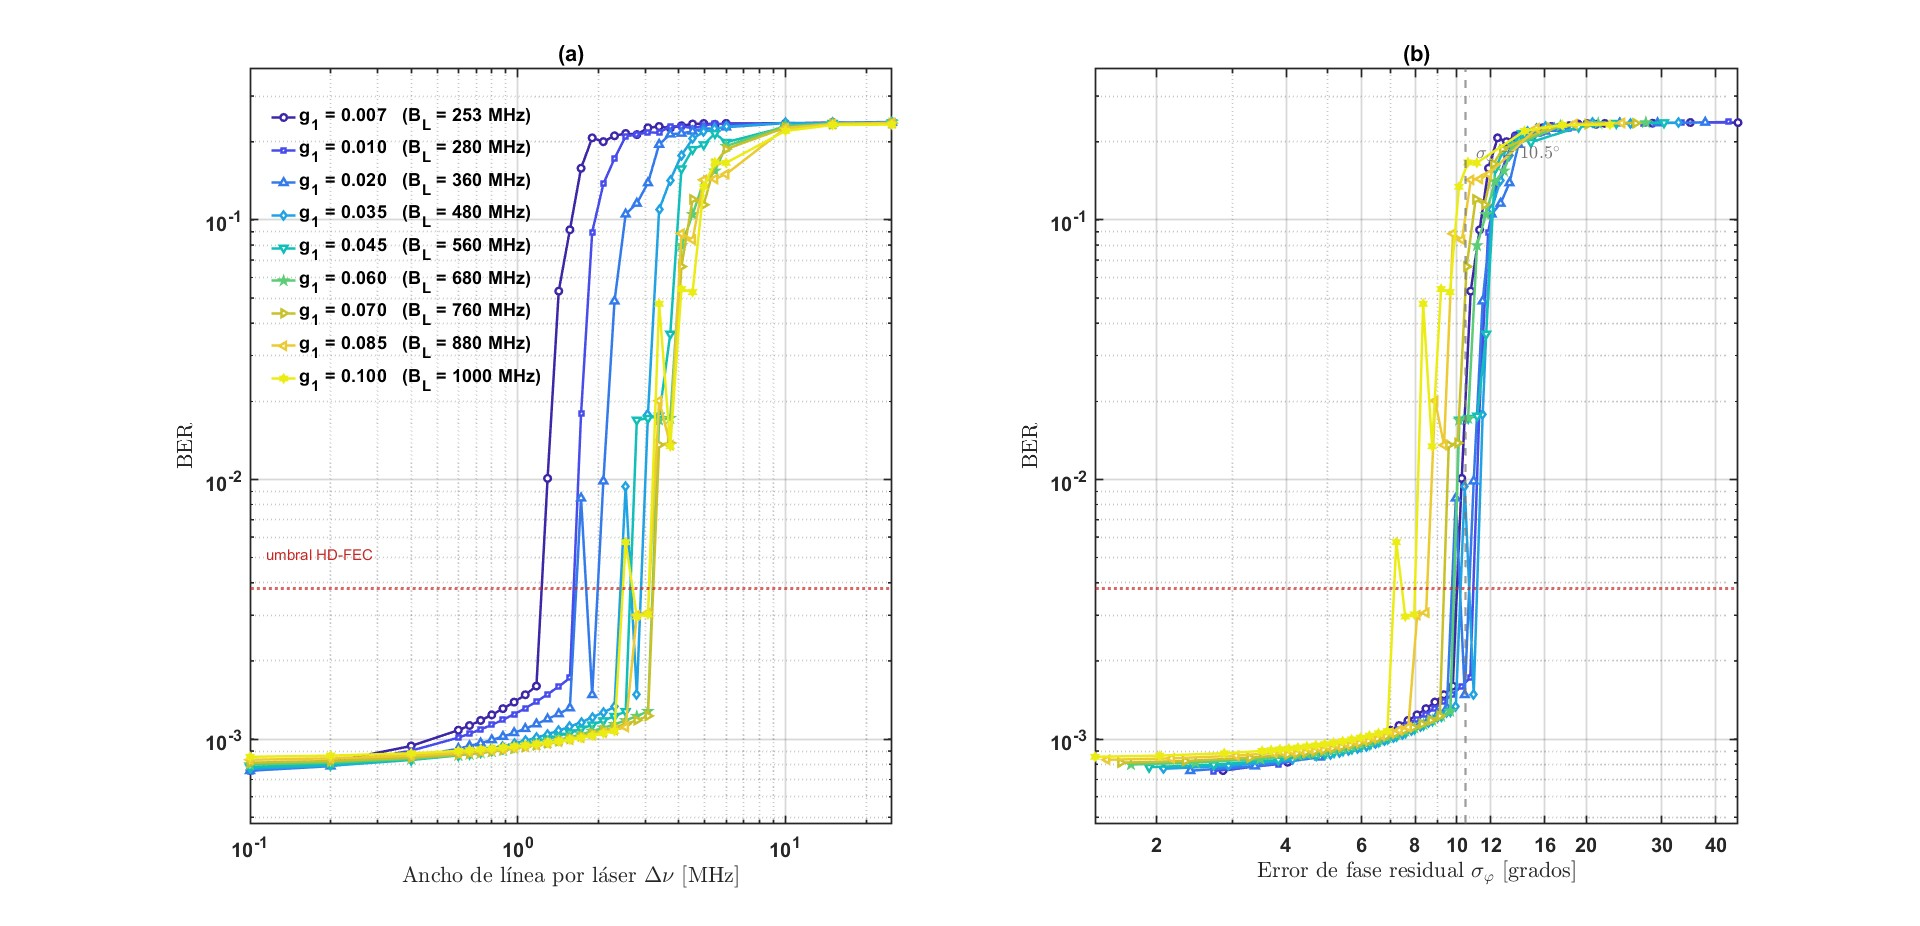
\includegraphics[width=0.98\textwidth]{figuras/TolAnchoLineaLey.jpg}
  \caption[Verificaci\'on de la ley de ruido de fase]{%
    (a) BER contra ancho de l\'inea por l\'aser, una curva por cada valor de
    $g_1$, a $\OSNR = \SI{14.4}{\dB}$. (b) Las mismas curvas contra el error
    de fase residual de la \cref{eq:var-fase}. Si la ley vale, todas tienen
    que cruzar el umbral en el mismo punto del eje horizontal.}
  \label{fig:tol-ley}
\end{figure}

El colapso se verifica sobre las seis curvas de menor ganancia, con
$\sigma_\varphi = \ang{10.5}$ y una dispersi\'on del \SI{5}{\percent}.

Este valor se interpreta contra el margen angular de QPSK, que es de
$\pm\ang{45}$. El cociente entre los dos vale
\begin{equation}
  \frac{\ang{45}}{\sigma_\varphi} = \num{4.3},
  \label{eq:cuatro-sigma}
\end{equation}
es decir que el receptor falla justo donde la cola de la distribuci\'on de
fase empieza a cruzar la frontera de decisi\'on con probabilidad apreciable.
Como muestra la \cref{sec:tol-laser-osnr}, ese cociente no es universal,
porque depende de la OSNR.

\begin{table}[htbp]
  \centering
  \begin{tabular}{lccc}
    \toprule
    $g_1$ & $B_L$ & $\dnu$ de quiebre [\si{\mega\hertz}] & $\sigma_\varphi$ \\
    \midrule
    \num{0.0067} & \SI{253}{\mega\hertz}  & \num{1.22} & \ang{9.96}  \\
    \num{0.010}  & \SI{280}{\mega\hertz}  & \num{1.60} & \ang{10.87} \\
    \num{0.020}  & \SI{360}{\mega\hertz}  & \num{1.97} & \ang{10.63} \\
    \num{0.035}  & \SI{480}{\mega\hertz}  & \num{2.86} & \ang{11.08} \\
    \num{0.045}  & \SI{560}{\mega\hertz}  & \num{2.61} & \ang{9.80}  \\
    \num{0.060}  & \SI{680}{\mega\hertz}  & \num{3.16} & \ang{9.79}  \\
    \midrule
    \num{0.070}  & \SI{760}{\mega\hertz}  & \num{3.17} & \ang{9.28}  \\
    \num{0.085}  & \SI{880}{\mega\hertz}  & \num{3.09} & \ang{8.51}  \\
    \num{0.100}  & \SI{1000}{\mega\hertz} & \num{3.08} & \ang{7.97}  \\
    \bottomrule
  \end{tabular}
  \caption[Ancho de l\'inea de quiebre contra la ganancia del lazo]{%
    Ancho de l\'inea de quiebre y desviaci\'on de fase residual que resulta,
    a $\OSNR = \SI{14.4}{\dB}$. Las seis primeras filas son las que cumplen
    la ley. Las \'ultimas tres se apartan, con un quiebre que deja de
    crecer y un $\sigma_\varphi$ que baja de forma monot\'ona.}
  \label{tab:tol-linewidth}
\end{table}

La \cref{tab:tol-linewidth} recorre las nueve ganancias ensayadas, con el
ancho de l\'inea de quiebre que resulta en cada una. La elecci\'on de la
ganancia de operaci\'on se discute en la \cref{sec:tol-laser-diseno}.

\subsection{Alcance y punto de dise\~no}
\label{sec:tol-laser-diseno}

Las \'ultimas tres filas de la \cref{tab:tol-linewidth} se apartan de la
ley. El quiebre se queda en unos \SI{3.1}{\mega\hertz} aunque el ancho de
banda del lazo siga creciendo.

\begin{figure}[H]
  \centering
  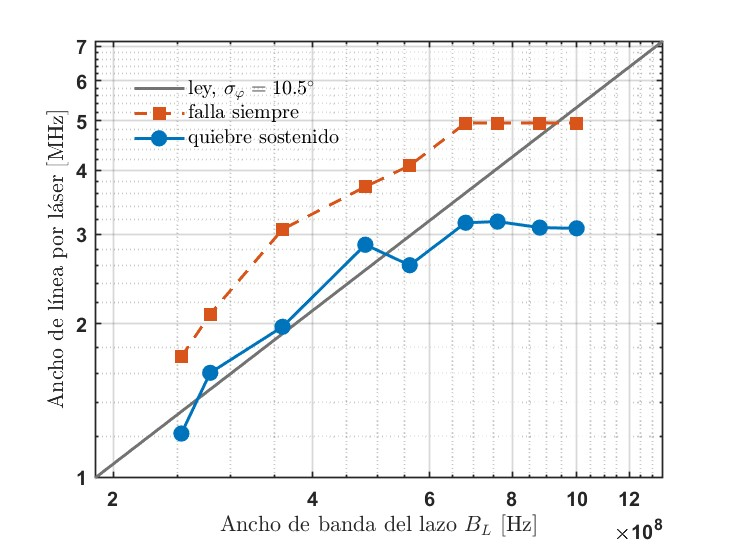
\includegraphics[width=0.72\textwidth]{figuras/TolAnchoLineaDiseno.jpg}
  \caption[Alcance de la ley de escala]{%
    Ancho de l\'inea de quiebre contra ancho de banda del lazo, con la recta
    de la ley ajustada sobre las curvas que la cumplen. Se agrega el ancho de
    l\'inea a partir del cual fallan todas las semillas. Entre las dos curvas
    se encuentra la banda en la que el receptor funciona o no seg\'un la
    realizaci\'on del ruido.}
  \label{fig:tol-diseno}
\end{figure}

La separaci\'on entre las dos curvas de la \cref{fig:tol-diseno} es la zona de
transici\'on. La falla no es una degradaci\'on sino un deslizamiento de ciclo, o cycle slip,
de modo que no hay un umbral duro sino una probabilidad creciente. Con
$g_1 = \num{0.02}$ el receptor empieza a fallar de forma aislada en
\SI{1.97}{\mega\hertz} y falla siempre a partir de \SI{3.07}{\mega\hertz}.

En la \cref{fig:tol-dosg1} se analizan dos valores de ganancia, con sus puntos de quiebre para una familia de OSNR.

\begin{figure}[H]
  \centering
  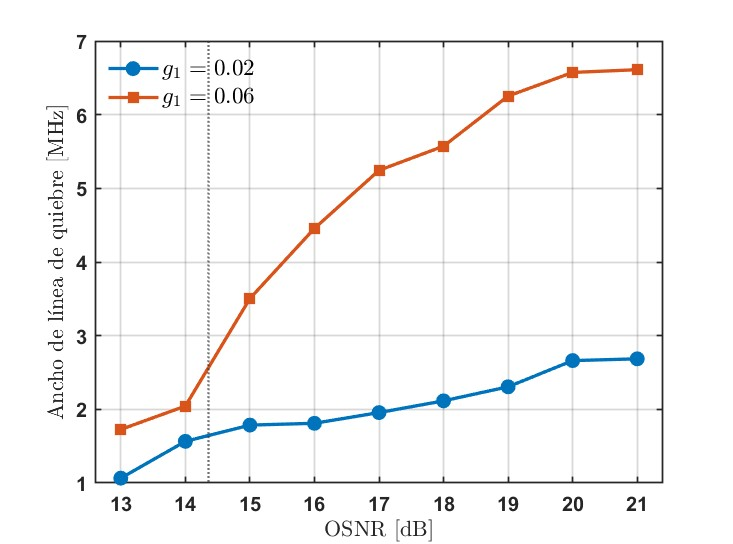
\includegraphics[width=0.72\textwidth]{figuras/TolAnchodeLineaDosValG1.jpg}
  \caption[Quiebre contra OSNR para dos ganancias de lazo]{%
    Ancho de l\'inea de quiebre contra OSNR, para dos valores de ganancia. Las dos curvas crecen con la OSNR y
    la del lazo ancho crece m\'as r\'apido.}
  \label{fig:tol-dosg1}
\end{figure}

Entre \SI{13}{\dB} y \SI{21}{\dB} el quiebre de $g_1 = \num{0.02}$ mejora un
factor \num{2.5}, mientras que el de $g_1 = \num{0.06}$ mejora un factor
\num{3.8}. El lazo ancho se beneficia m\'as de bajar el ASE. Esto indica que lo
que lo limita a OSNR baja es el ruido aditivo que integra, y no un l\'imite
propio del lazo. Si fuese as\'i, el quiebre de
$g_1 = \num{0.06}$ se habr\'ia mantenido constante al mejorar la OSNR. A 
OSNR alta la mejora es cada vez menor por \si{\dB} de OSNR. En este caso el factor de falla predominante es el l\'imite propio del lazo, es decir, su ancho de banda, en lugar del ruido aditivo.

Se concluye que pasar de \num{0.02} a \num{0.06} sube la tolerancia un factor
\num{1.6}, en lugar del \num{1.9} que predice el ajuste de la
\cref{fig:tol-diseno}.

Con esto queda fijado el punto de dise\~no. La ganancia del lazo de fase se
fij\'o en $g_1 = \num{0.06}$, que por las expresiones de la
\cref{sec:dsp-cpr} corresponde a $B_L = \SI{680}{\mega\hertz}$ y a un
amortiguamiento de $\zeta = \num{0.77}$. 

Hacia valores menores de $B_L$, la tolerancia se pierde en proporci\'on con \'el, tal como
predice la \cref{eq:var-fase}. Hacia valores mayores, y a OSNR constante, satura porque el lazo pasa a
integrar m\'as ruido aditivo del que gana en seguimiento de la fase. Con esta
ganancia el receptor tolera \SI{3.16}{\mega\hertz} de ancho de l\'inea por
l\'aser, de modo que contra el requisito de \SI{100}{\kilo\hertz} el margen es
de un factor \num{32}. El l\'aser del laboratorio, de \SI{15}{\kilo\hertz},
est\'a un factor \num{210} por debajo del quiebre.

\subsection{Ruido de intensidad relativa}
\label{sec:tol-rin}

El ruido de intensidad se barri\'o con la misma familia de OSNR, como se ve en la \cref{fig:tol-rin}. La respuesta es plana desde
\SI{-165}{\dB\per\hertz} hasta \SI{-140}{\dB\per\hertz}, que es el valor de los l\'aseres
utilizados, y el desempe\~no empieza a degradarse reci\'en en
\SI{-130}{\dB\per\hertz}. El cruce del umbral va de \SI{-120}{\dB\per\hertz}
en \SI{13}{\dB} de OSNR a \SI{-109}{\dB\per\hertz} desde \SI{17}{\dB} en
adelante.


\begin{figure}[H]
  \centering
  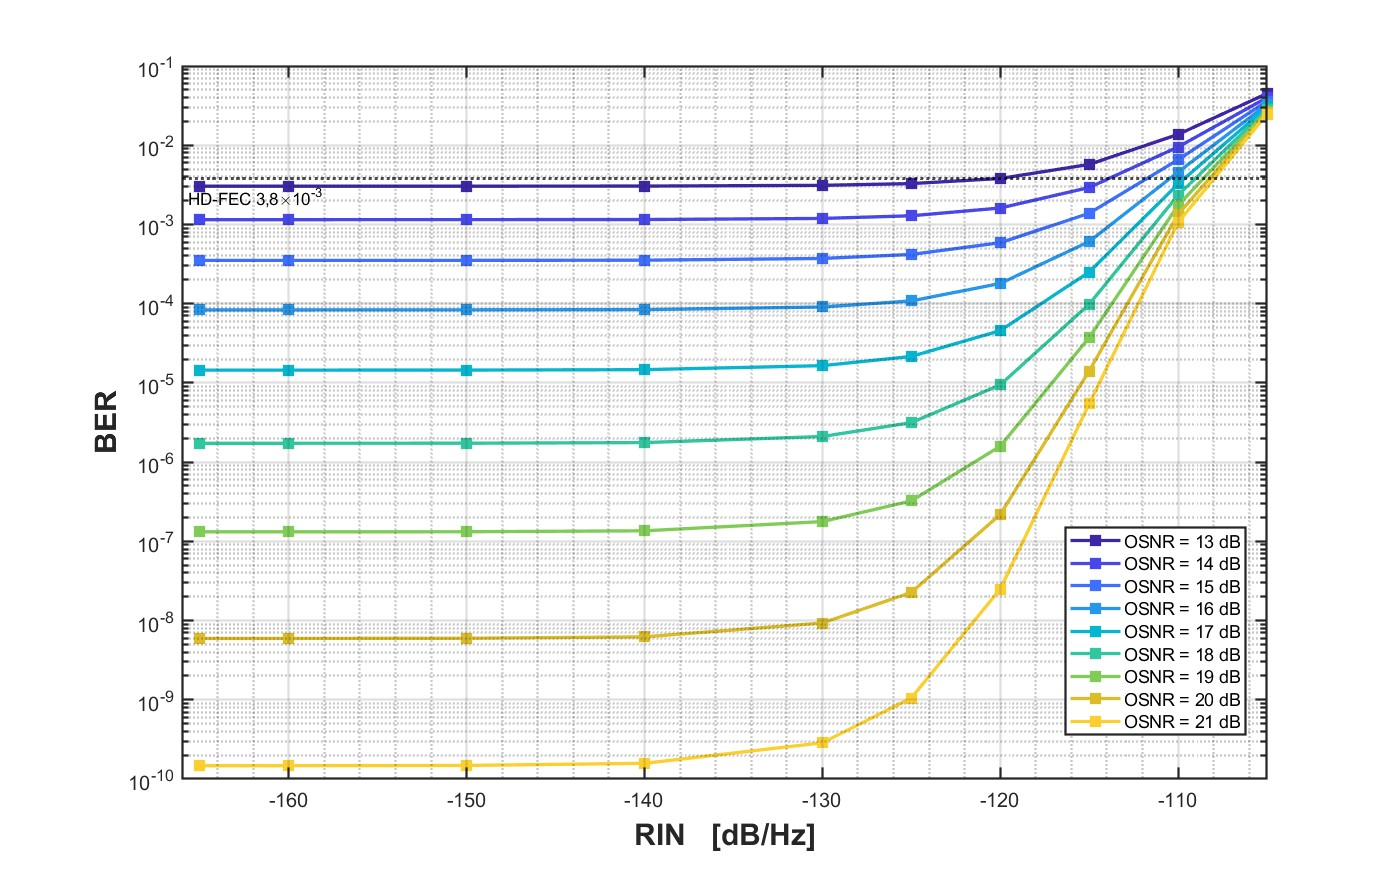
\includegraphics[width=0.92\textwidth]{figuras/BarridoRINOSNR.jpg}
  \caption[Tolerancia al RIN]{%
    BER en funci\'on del RIN del l\'aser, para una familia de
    nueve valores de OSNR. El color determina la OSNR en pasos de \SI{1}{\dB}, de azul oscuro en \SI{13}{\dB} a amarillo en \SI{21}{\dB}.}
  \label{fig:tol-rin}
\end{figure}

El RIN degrada el desempe\~no de forma gradual, con un l\'imite que mejora al
bajar el ASE y se aplana por encima de \SI{17}{\dB}. El margen contra el
componente real es amplio en todo el rango simulado.

\section{Deterioros del front end del receptor}
\label{sec:tol-frontend}

En esta secci\'on se analizan los deterioros provenientes del
receptor para encontrar sus tolerancias m\'aximas.

\paragraph{Skew entre las ramas}
El skew es la diferencia de retardo entre los cuatro carriles del front end, y
es el \'unico deterioro de este cap\'itulo cuyo margen es estrecho. Con el
estimador de frecuencia desactivado el ecualizador lo absorbe hasta
\SI{62.5}{\pico\second}. Pero con el estimador de frecuencia activo, que es la condici\'on
real de operaci\'on, la tolerancia cae a \SI{4.5}{\pico\second} para
\SI{0.5}{\dB} de penalidad.

Esto es debido al orden en que est\'an los bloques. Un retardo $\tau$ entre la rama en
fase y la de cuadratura es una operaci\'on ampliamente lineal sobre la se\~nal
compleja: si $x$ es la se\~nal sin deteriorar, la que llega al conversor es
\begin{equation}
  r = A(f)\,x + B(f)\,x^{*},
  \qquad
  \left|\frac{B(f)}{A(f)}\right| = \left|\tan(\pi f \tau)\right|,
  \label{eq:tol-skew-wl}
\end{equation}
con una r\'eplica conjugada que crece hacia los bordes de la banda. El
ecualizador mariposa de este receptor es de filtros reales y espaciado $T/2$,
de modo que tiene los grados de libertad para cancelar la r\'eplica. Es decir, puede
aplicar retardos distintos a la componente en fase y a la de cuadratura, lo que ocurre con el
estimador desactivado, llegando a \SI{62.5}{\pico\second} de tolerancia.

La compensaci\'on de frecuencia multiplica la se\~nal por $e^{-j\omega t}$.
Sin embargo, sobre la r\'eplica
conjugada deja un factor $e^{-j2\omega t}$. El efecto neto es que deja de estar en la frecuencia espejo y pasa a girar a $2\Delta f$ respecto de la se\~nal. Es un deterioro que se vuelve irreversible, porque la cancelaci\'on exige que los coeficientes del ecualizador se adapten a esa velocidad.

\begin{table}[htbp]
  \centering

  \begin{tabular}{lcccc}
    \toprule
    & \multicolumn{4}{c}{Skew entre ramas} \\
    \cmidrule(l){2-5}
    & \SI{0}{\pico\second} & \SI{2}{\pico\second} & \SI{5}{\pico\second}
    & \SI{10}{\pico\second} \\
    \midrule
    $\Df = 0$                      & 35,10 & 35,09 & 35,10 & 35,12 \\
    \midrule
    $\Df = \SI{0.02}{\giga\hertz}$ & 35,10 & 35,31 & 36,66 & colapsa \\
    $\Df = \SI{0.2}{\giga\hertz}$  & 35,10 & 35,47 & 37,44 & colapsa \\
    $\Df = \SI{1}{\giga\hertz}$    & 35,10 & 35,48 & 37,46 & colapsa \\
    $\Df = \SI{2}{\giga\hertz}$    & 35,10 & 35,46 & 37,32 & colapsa \\
    $\Df = \SI{4}{\giga\hertz}$    & 35,10 & 35,39 & 36,93 & colapsa \\
    \bottomrule
  \end{tabular}
  \caption[Origen del l\'imite de skew]{%
    EVM de la peor polarizaci\'on contra skew entre las ramas en fase y
    cuadratura, con el estimador de frecuencia activo, para seis valores de
    offset, a $\OSNR = \SI{14.4}{\dB}$. En la primera fila el offset es nulo y el ecualizador absorbe el
    skew en todo el rango barrido.}
  \label{tab:tol-skew}
\end{table}

La \cref{tab:tol-skew} muestra un an\'alisis de los dos efectos mencionados. Entre
\SI{0.2}{\giga\hertz} y \SI{4}{\giga\hertz} el
colapso sigue cayendo en \SI{10}{\pico\second} y el EVM en
\SI{5}{\pico\second} se mantiene aproximadamente constante. Esto significa que, desde offsets de 
frecuencia peque\~nos como \SI{20}{\mega\hertz}, los coeficientes del ecualizador no llegan a adaptarse, es decir, la penalidad satura desde el principio. Con offset nulo no se tiene una componente espuria rotando, y el ecualizador absorbe el skew hasta los \SI{62.5}{\pico\second} del barrido, al igual que con el bloque desactivado.


El problema, entonces, no es de grados de libertad sino de orden. Una forma de
resolverlo es compensar el skew y el desbalance de cuadratura antes del
recuperador de frecuencia, con una estructura ampliamente lineal
dedicada~\cite{portodasilva2016}, en el punto de la cadena donde la r\'eplica
conjugada todav\'ia est\'a quieta. Esto implicar\'ia reordenar la cadena del
DSP y rehacer los an\'alisis correspondientes.

Con la cadena actual, es necesario hacer una calibraci\'on del front end receptor antes de entrar en operaci\'on. El skew tiene que quedar por debajo de
\SI{4.5}{\pico\second} para tener una penalidad menor a \SI{0.5}{\dB}.


\paragraph{Error de reloj}
El desajuste entre el reloj del transmisor y el del ADC del receptor se tolera
hasta \SI{175}{\ppm}. El l\'imite lo impone el rango de enganche del lazo de
segundo orden, no la longitud de la secuencia de s\'imbolos. Un desajuste de reloj mueve el
instante de muestreo un poco por s\'imbolo, siempre en el mismo sentido, de
modo que el corrimiento se acumula a lo largo de la simulaci\'on. A
\SI{175}{\ppm} ese corrimiento pasa de \num{8.8} per\'iodos de s\'imbolo en una
secuencia de \num{5e4} a \num{70} en uno de \num{4e5}. Repitiendo el barrido en
todo ese rango el punto de falla no se mueve, lo que descarta al corrimiento
acumulado como causa. Contra los \SI{25.55}{\ppm} que impone el Doppler sobre
la tasa de s\'imbolos, el margen es de un factor \num{6.8}, y deja unos
\SI{150}{\ppm} de presupuesto para la deriva del oscilador del receptor.

\paragraph{Fase de muestreo, error de cuadratura y desbalance de ganancia}
Ninguno de los tres impone l\'imite en el rango explorado. El desajuste de fase
de muestreo se barri\'o hasta $1{,}0\,\Ts$, es decir un s\'imbolo completo,
sin penalidad medible.
El error de cuadratura del h\'ibrido se barri\'o hasta \SI{18}{\degree} con el
mismo resultado, porque la ortogonalizaci\'on de Gram-Schmidt lo invierte de
forma exacta, seg\'un se mostr\'o en la \cref{sec:dsp-gsop}.
El desbalance de ganancia entre las ramas tiene un resultado similar. Se barri\'o
hasta un cociente de \num{0.30}, es decir un factor tres entre las dos
ramas, sin penalidad medible.


\section{Presupuesto conjunto de deterioros}
\label{sec:tol-presupuesto}

En las secciones anteriores se midi\'o cada deterioro por separado. Esta secci\'on analiza diferentes casos con distintas configuraciones de deterioros, a trav\'es de un barrido sobre nueve valores de OSNR.

Se midieron trece configuraciones, numeradas de \Cfg{0} a \Cfg{12} y definidas
en la \cref{tab:tol-configs}. Todas comparten el mismo punto de partida, que es
el receptor con el l\'aser nominal de \SI{100}{\kilo\hertz} y el offset
Doppler de \SI{2}{\giga\hertz} que usa todo el cap\'itulo, y se distinguen por
lo que se agrega encima.

\Cfg{0} es ese punto de partida sin nada agregado y sirve de referencia para
todos los dem\'as casos. De \Cfg{1} a \Cfg{3} se activa un deterioro por vez, con
niveles calibrados de antemano para que los tres cuesten lo mismo por separado:
ancho de l\'inea de \SI{1.333}{\mega\hertz}, deriva de polarizaci\'on de
\SI{14.53}{\mega\radian\per\second} y skew de \SI{3.789}{\pico\second}. De
\Cfg{4} a \Cfg{7} se combinan esos mismos tres niveles de a pares y de a
tres.

Por otro lado, los cinco \'ultimos casos usan los valores de especificaci\'on del
enlace.
\Cfg{8} agrega los dos deterioros que var\'ian a lo largo del pase, la deriva
de polarizaci\'on y el error de cuadratura del h\'ibrido. \Cfg{9} agrega los
cuatro que son valores fijos de especificaci\'on, el Doppler, el error de
reloj, el desajuste de fase de muestreo y el skew. \Cfg{10} tiene todos los deterioros a
la vez, mostrando el peor caso de vuelo. \Cfg{11} y \Cfg{12} repiten \Cfg{10} con el
skew calibrado a \SI{2}{\pico\second} y \SI{0}{\pico\second}.

\begin{table}[htbp]
  \centering
  \small
  \setlength{\tabcolsep}{4.5pt}

  \begin{tabular}{llccccccc}
    \toprule
    & & $\dnu$ & SOP & $\varphi$ & $\Df$ & reloj & fase & skew \\
    & & [\si{\kilo\hertz}] & [\si{\radian\per\second}] & [\si{\degree}]
      & [\si{\giga\hertz}] & [\si{\ppm}] & [$\Ts$] & [\si{\pico\second}] \\
    \midrule
    \Cfg{0}    & referencia        & ---  & ---        & --- & --- & ---   & ---  & ---  \\
    \midrule
    \Cfg{1}    & \multirow{7}{*}{\parbox{2.6cm}{niveles\\calibrados}}
                                   & 1333 & ---        & --- & --- & ---   & ---  & ---  \\
    \Cfg{2}    & & ---  & \num{1.453e7} & --- & --- & ---   & ---  & ---  \\
    \Cfg{3}   & & ---  & ---          & --- & --- & ---   & ---  & 3,79 \\
    \Cfg{4} & & 1333 & \num{1.453e7} & --- & --- & ---   & ---  & ---  \\
    \Cfg{5}  & & 1333 & ---          & --- & --- & ---   & ---  & 3,79 \\
    \Cfg{6}   & & ---  & \num{1.453e7} & --- & --- & ---   & ---  & 3,79 \\
    \Cfg{7}  & & 1333 & \num{1.453e7} & --- & --- & ---   & ---  & 3,79 \\
    \midrule
    \Cfg{8}   & \multirow{5}{*}{\parbox{2.6cm}{valores\\de vuelo}}
                                   & ---  & \num{e-3}  & 3   & --- & ---   & ---  & ---  \\
    \Cfg{9}  & & ---  & ---        & --- & 6   & 25,55 & 0,25 & 5    \\
    \Cfg{10}   & & ---  & \num{e-3}  & 3   & 6   & 25,55 & 0,25 & 5    \\
    \Cfg{11}   & & ---  & \num{e-3}  & 3   & 6   & 25,55 & 0,25 & 2    \\
    \Cfg{12}   & & ---  & \num{e-3}  & 3   & 6   & 25,55 & 0,25 & ---  \\
    \bottomrule
  \end{tabular}
  \caption[Configuraciones de deterioros del presupuesto]{%
    Las trece configuraciones del presupuesto. Un gui\'on indica que el
        deterioro est\'a en su valor neutro, es decir ausente, salvo en las
    columnas de $\dnu$ y $\Df$, donde significa que se mantiene el valor
    base de todo el cap\'itulo, \SI{100}{\kilo\hertz} de ancho de l\'inea por
    l\'aser y \SI{2}{\giga\hertz} de offset Doppler.}
  \label{tab:tol-configs}
\end{table}

\begin{figure}[H]
  \centering
  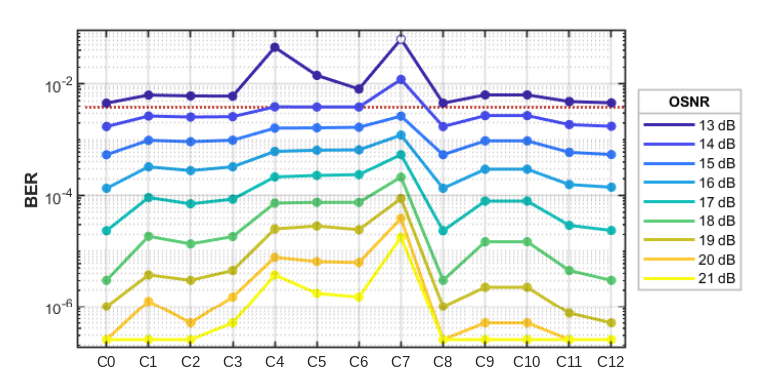
\includegraphics[width=0.95\textwidth]{figuras/tol_ber_vs_deterioro.png}
  \caption[BER de cada configuraci\'on de deterioros]{%
    BER de las trece configuraciones de la \cref{tab:tol-configs} para la
    familia de OSNR simuladas, de \SIrange{13}{21}{\dB}. El color determina la
    OSNR, de azul oscuro en \SI{13}{\dB} a amarillo en \SI{21}{\dB}.}
  \label{fig:tol-familia}
\end{figure}

La \cref{fig:tol-familia} pone las trece configuraciones una al lado de la
otra para las nueve OSNR de \SIrange{13}{21}{\dB}. El orden entre ellas es el
mismo en el resto de figuras, as\'i que alcanza con resumir cada configuraci\'on por la OSNR
a la que cruza el umbral HD-FEC.

\begin{figure}[H]
  \centering
  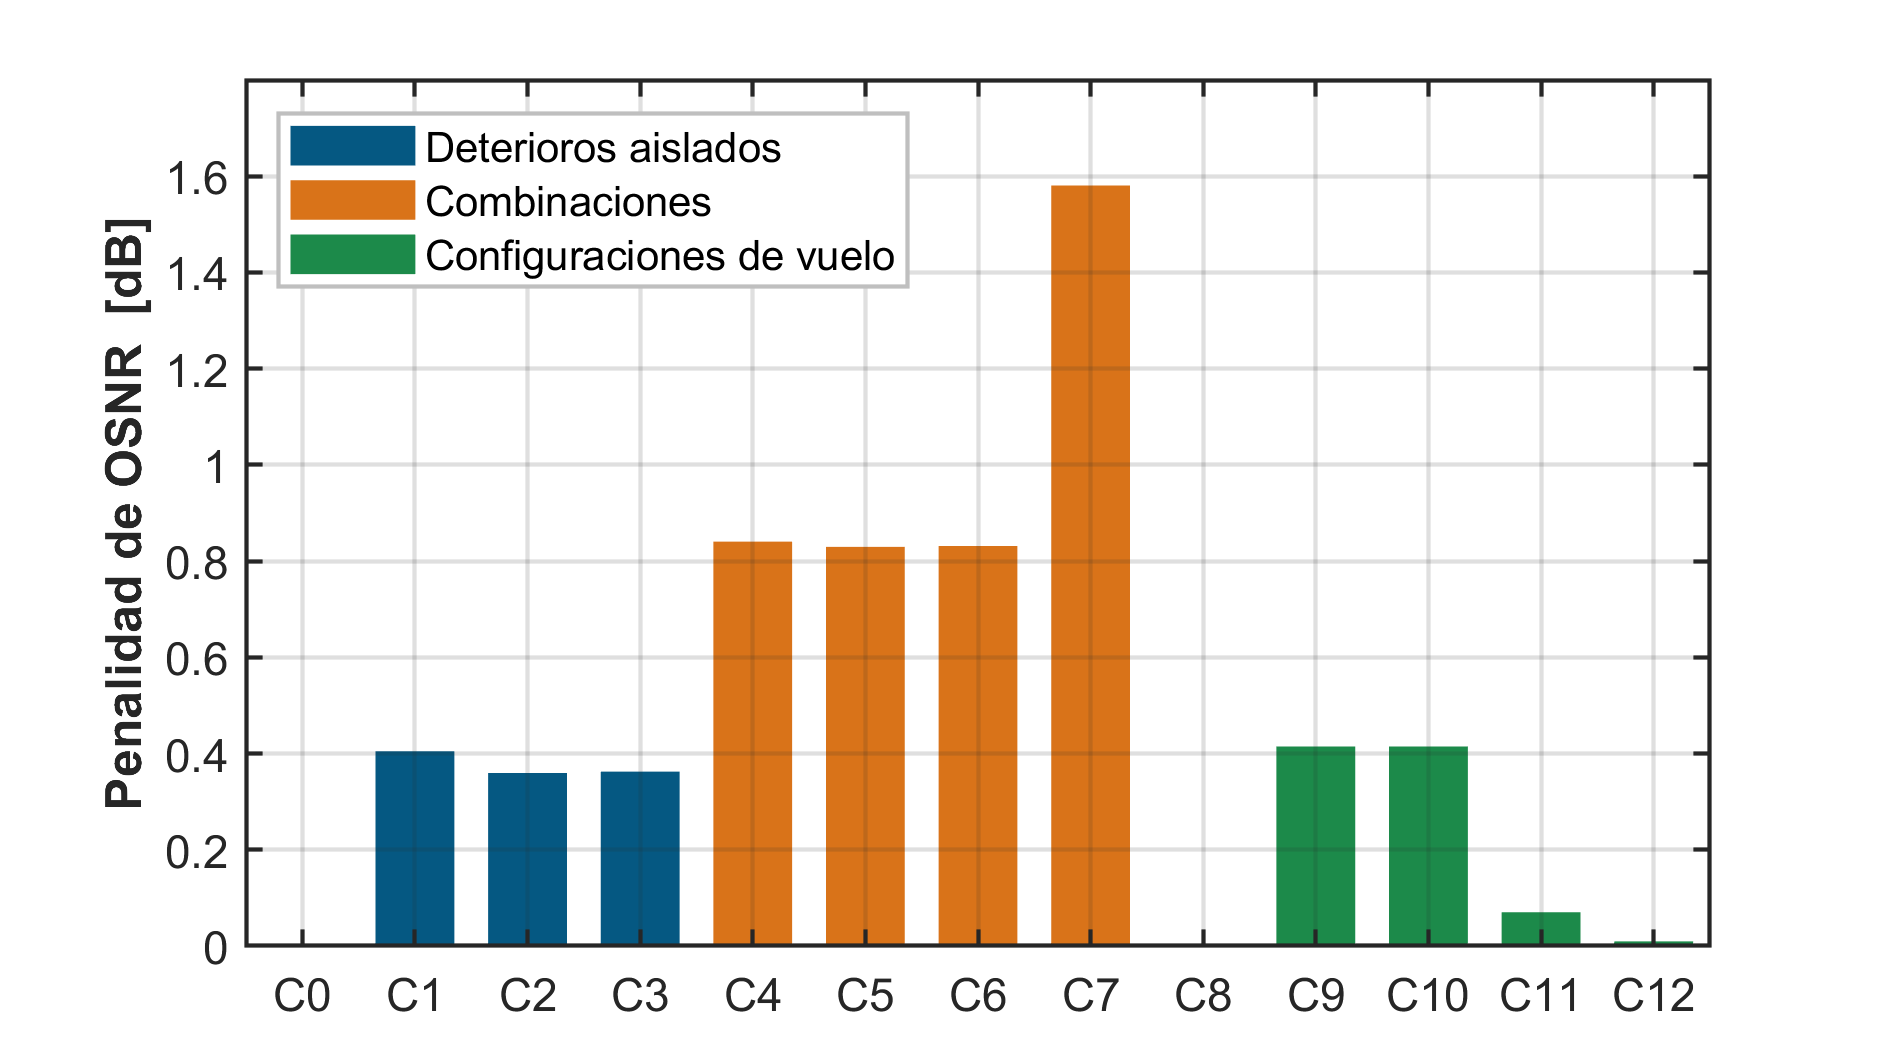
\includegraphics[width=0.95\textwidth]{figuras/tol_penalidad_configuraciones.png}
  \caption[Penalidad de OSNR por configuraci\'on]{%
    Penalidad de OSNR en el cruce del umbral HD-FEC, por configuraci\'on,
    respecto de \Cfg{0}. Los tres deterioros calibrados de \Cfg{1} a \Cfg{3}
    entran con el mismo peso, los pares de \Cfg{4} a \Cfg{6} son aditivos y
    \Cfg{7} es superaditiva.}
  \label{fig:tol-penalidad}
\end{figure}

La distancia entre el cruce medido y el de \Cfg{0} es lo que cuesta la
configuraci\'on. Estos valores se muestran en la \cref{fig:tol-penalidad} y en la
\cref{tab:tol-presupuesto}.

\begin{table}[htbp]
  \centering

  \begin{tabular}{llcc}
    \toprule
    & Deterioros activos & $\OSNR$ de cruce & Penalidad \\
    \midrule
    \Cfg{0}  & ninguno                   & \SI{13.18}{\dB} & ---             \\
    \midrule
    \Cfg{1}  & ancho de l\'inea          & \SI{13.58}{\dB} & \SI{0.40}{\dB}  \\
    \Cfg{2}  & deriva de polarizaci\'on  & \SI{13.54}{\dB} & \SI{0.36}{\dB}  \\
    \Cfg{3}  & skew                      & \SI{13.54}{\dB} & \SI{0.36}{\dB}  \\
    \midrule
    \Cfg{4}  & ancho de l\'inea y SOP    & \SI{14.02}{\dB} & \SI{0.84}{\dB}  \\
    \Cfg{5}  & ancho de l\'inea y skew   & \SI{14.01}{\dB} & \SI{0.83}{\dB}  \\
    \Cfg{6}  & SOP y skew                & \SI{14.01}{\dB} & \SI{0.83}{\dB}  \\
    \Cfg{7}  & los tres                  & \SI{14.76}{\dB} & \SI{1.58}{\dB}  \\
    \midrule
    \Cfg{8}  & vuelo, los que var\'ian   & \SI{13.18}{\dB} & \SI{0.00}{\dB}  \\
    \Cfg{9}  & vuelo, los fijos          & \SI{13.59}{\dB} & \SI{0.41}{\dB}  \\
    \Cfg{10} & vuelo completo            & \SI{13.59}{\dB} & \SI{0.41}{\dB}  \\
    \Cfg{11} & vuelo, skew \SI{2}{\pico\second} & \SI{13.25}{\dB} & \SI{0.07}{\dB} \\
    \Cfg{12} & vuelo, skew \SI{0}{\pico\second} & \SI{13.19}{\dB} & \SI{0.01}{\dB} \\
    \bottomrule
  \end{tabular}
  \caption[Presupuesto conjunto de deterioros]{%
    OSNR a la que cruza el umbral HD-FEC cada una de las configuraciones de
    la \cref{tab:tol-configs}, y penalidad respecto de \Cfg{0}.}
  \label{tab:tol-presupuesto}
\end{table}

De la tabla salen cuatro resultados.
\begin{puntos}
  \item La calibraci\'on cumple su prop\'osito: \Cfg{1}, \Cfg{2} y \Cfg{3}
        dan \num{0.40}, \num{0.36} y \SI{0.36}{\dB}. Los tres deterioros
        aislados pesan casi lo mismo, que era la condici\'on para poder
        compararlos de igual a igual.

  \item Los pares se apartan ligeramente de la suma lineal: \Cfg{4}, \Cfg{5} y
        \Cfg{6} dan \num{0.84}, \num{0.83} y \SI{0.83}{\dB}, contra los
        \SIrange{0.72}{0.76}{\dB} que predice la suma. El
        exceso ronda la d\'ecima de decibel en los tres casos. Se hace notar tambi\'en
        que los tres pares coinciden entre s\'i, lo que dice que ninguna
        combinaci\'on tiene mayor peso.

  \item Con los tres juntos el exceso se vuelve mayor: \Cfg{7} cuesta
        \SI{1.58}{\dB} contra \SI{1.12}{\dB} de la suma lineal.  Esto puede
        deberse a que los tres se corrigen con lazos que dependen de la
        decisi\'on. Cuando uno de ellos empeora las decisiones, los otros dos
        adaptan peor.

  \item El peor caso de vuelo es dominado por el skew: \Cfg{8} agrega la deriva de polarizaci\'on del pase y
        \SI{3}{\degree} de error de cuadratura. El resultado en este caso es id\'entico 
        al de \Cfg{0} en las nueve OSNR, porque la deriva real est\'a
        diez \'ordenes por debajo del quiebre y el error de cuadratura lo
        invierte la ortogonalizaci\'on. \Cfg{9} tiene una penalidad de \SI{0.41}{\dB}, todo debido al skew. 
        Sin skew, que es \Cfg{12}, la
        penalidad cae a \SI{0.01}{\dB}. Con \SI{2}{\pico\second}, que es
        \Cfg{11}, queda en \SI{0.07}{\dB}. Por eso \Cfg{9} y \Cfg{10} dan el
        mismo n\'umero. Lo que \Cfg{10} agrega sobre \Cfg{9} es justamente lo
        que \Cfg{8} muestra que no tiene penalidad.
\end{puntos}

\begin{figure}[H]
  \centering
  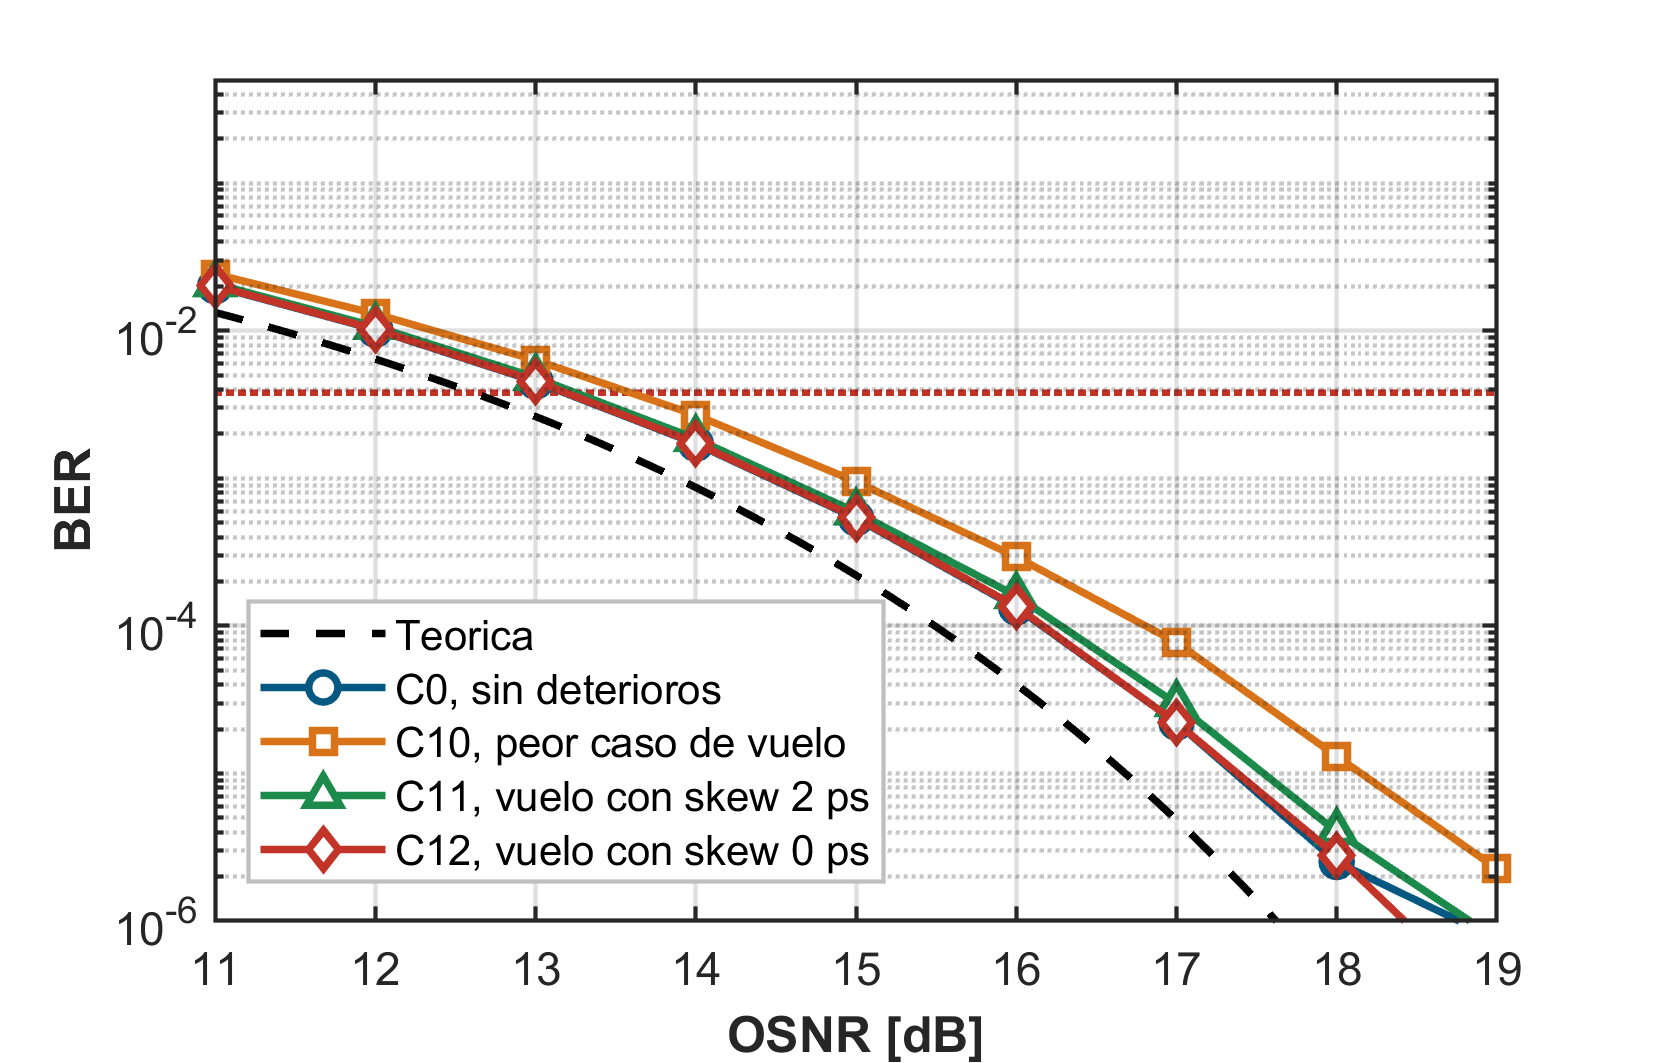
\includegraphics[width=0.85\textwidth]{figuras/tol_vuelo_ber_vs_osnr.png}
  \caption[Configuraciones de vuelo contra el receptor sin deterioros]{%
    BER contra OSNR de \Cfg{10}, \Cfg{11} y \Cfg{12}, comparadas con \Cfg{0} y
    con la curva te\'orica de DP-QPSK. La separaci\'on entre \Cfg{10} y
    \Cfg{0} es de \SI{0.41}{\dB} en el umbral, y desaparece casi por completo
    al reducir el skew del front end. La distancia entre la curva te\'orica y
    \Cfg{0} es la penalidad de implementaci\'on.}
  \label{fig:tol-vuelo}
\end{figure}

La \cref{fig:tol-vuelo} muestra las curvas BER para las tres \'ultimas configuraciones. Con el skew calibrado, el
ancho de l\'inea y la deriva de polarizaci\'on de especificaci\'on no imponen una penalidad significativa. El skew es el \'unico deterioro que importa en el presupuesto de vuelo,
lo que refuerza el requisito de calibraci\'on de la
\cref{sec:tol-frontend}.


\section{Conclusiones}
\label{sec:tol-conclusiones}

La \cref{tab:tol-final} re\'une todo el cap\'itulo. En ella se muestra, para cada deterioro, el
valor que impone el canal o el componente, la tolerancia medida y el margen
entre los dos.

\begin{table}[htbp]
  \centering

  \begin{tabular}{llll}
    \toprule
    Deterioro & Valor del enlace & Tolerancia medida & Margen \\
    \midrule
    Offset Doppler            & \SI{\pm 6.0}{\giga\hertz}          & \SI{\pm 8.0}{\giga\hertz}        & \SI{\pm 2.0}{\giga\hertz}    \\
    Chirp Doppler             & \SI{6.55}{\mega\hertz\per\second}  & \SI{1.8e12}{\hertz\per\second}   & \num{2.7e5}  \\
    Deriva de SOP             & \SI{1e-3}{\radian\per\second}       & \SI{2.15e7}{\radian\per\second}  & \num{2.2e10} \\
    Ancho de l\'inea          & \SI{100}{\kilo\hertz}              & \SI{3.16}{\mega\hertz}           & \num{32}     \\
    Error de reloj            & \SI{25.55}{\ppm}        & \SI{175}{\ppm}        & \num{6.8}    \\
    Skew del front end$^{*}$  & \SI{5}{\pico\second}               & \SI{4.5}{\pico\second}           & \num{0.9}    \\
    Fase de muestreo$^{*}$    & $0{,}25\,\Ts$                     & $>1{,}0\,\Ts$                 & $>\num{4}$   \\
    Error de cuadratura$^{*}$ & \SI{3}{\degree}                    & $>\SI{18}{\degree}$              & $>\num{6}$   \\
    \bottomrule
  \end{tabular}
  \caption[Resumen de tolerancias y m\'argenes]{%
    Tolerancia medida de cada deterioro contra el valor que impone el enlace.
    El margen es el cociente entre los dos. Los deterioros marcados con
    asterisco son calibrables en la integraci\'on y no propiedades del canal.}
  \label{tab:tol-final}
\end{table}

Se obtienen las siguientes conclusiones:

En primer lugar, el receptor tiene margen de sobra contra todo lo que impone
el canal. El deterioro m\'as ajustado de los provenientes del enlace es el
offset Doppler, con un margen de \SI{\pm 2.0}{\giga\hertz} sobre el requisito de \SI{\pm 6.0}{\giga\hertz}, y el resto est\'a entre uno y diez
\'ordenes de magnitud por encima del valor f\'isico. Ning\'un deterioro del
canal satelital amenaza el funcionamiento del receptor a
\SI{32}{\giga\baud}.

Por otro lado, el \'unico margen realmente estrecho no viene del canal sino
del equipo del receptor. El skew entre las ramas del front end tolera
\SI{4.5}{\pico\second} contra los \SI{5}{\pico\second} de especificaci\'on, es
decir que est\'a en el l\'imite, y es adem\'as el t\'ermino que domina el
presupuesto de vuelo de la \cref{sec:tol-presupuesto}. Reducir el skew a \SI{2}{\pico\second} en la integraci\'on disminuir\'ia la penalidad total de vuelo de \num{0.41} a \SI{0.07}{\dB}, lo cual ser\'ia recomendable en la pr\'actica.

En tercer lugar, el l\'imite de captura de Doppler, que es el margen m\'as
ajustado del lado del canal, es lo que justifica la tasa de s\'imbolo elegida.
Las tres tasas presentan un l\'imite en $\Rs/4$, de modo que la ventana de captura crece con
la tasa, y s\'olo \SI{32}{\giga\baud} cubre el requisito de
\SI{\pm 6.0}{\giga\hertz} con margen. 

Por \'ultimo, los dos deterioros que vienen del movimiento del sat\'elite, el
offset y el chirp, se barrieron contra una familia de doce valores de OSNR y
en ninguno de los dos el quiebre se vio afectado por el ruido. La
\cref{fig:tol-frecuencia-estimada} muestra adem\'as que el estimador de
frecuencia sigue el offset sin error apreciable hasta el \'ultimo punto
te\'orico posible, y que pasado el l\'imite salta al valor que predice el
plegado de Nyquist. Esto significa que estas tolerancias no son un compromiso
entre se\~nal y ruido que se pueda compensar con potencia \'optica. Son
propiedades de los algoritmos y de la frecuencia a la que se los utiliza.
Ampliar estas tolerancias exige cambiar el procesamiento, subiendo las
muestras por s\'imbolo o reemplazando el elevado a la cuarta por un m\'etodo
sin ambig\"uedad, no mejorando el enlace \'optico.

En cambio, los ruidos del l\'aser se comportan diferente. Tanto el de fase como el de
intensidad degradan el desempe\~no de forma gradual, y sus l\'imites var\'ian con la
OSNR, porque la falla ocurre cuando el deterioro y el ruido \'optico juntos
agotan el presupuesto de error. En esos dos casos la potencia \'optica implica un aumento de la tolerancia. Con el ancho de banda del lazo adoptado, el receptor admite
\SI{3.16}{\mega\hertz} de ancho de l\'inea por l\'aser, un factor \num{32}
sobre el requisito, y el RIN no impone ninguna restricci\'on en todo el rango
simulado. 


% !TeX root = ../main.tex
%% =======================================================================
%  CAPITULO 8 — VALIDACION EXPERIMENTAL
\chapter{Validaci\'on experimental}
\label{cap:experimental}

\section{Introducci\'on}
\label{sec:exp-intro}

En este cap\'itulo se implementa la cadena \'optica en el laboratorio y se
procesan las se\~nales adquiridas utilizando la misma cadena DSP desarrollada
y evaluada mediante simulaciones en los cap\'itulos anteriores.

El objetivo es validar experimentalmente el procesamiento digital, no
reproducir el enlace satelital completo. El sistema implementado consiste en
un enlace de fibra \'optica entre un transmisor y un receptor coherente, por
lo que no contempla efectos como la p\'erdida de espacio libre, la
amplificaci\'on \'optica de potencia o la rotaci\'on din\'amica del estado de
polarizaci\'on. Sin embargo, permite evaluar el desempe\~no del DSP frente a
imperfecciones reales de los dispositivos, que en las simulaciones se
representan mediante modelos aproximados. Entre ellas se encuentran el ruido
de fase de los l\'aseres, los desbalances y las limitaciones de ancho de banda
del front end, el desfasaje temporal entre canales y las imperfecciones del
proceso de adquisici\'on.

La validaci\'on experimental comprende tres ensayos. El primero eval\'ua el
desempe\~no del receptor para tres tasas de s\'imbolo, \SI{12.5}{\giga\baud},
\SI{25}{\giga\baud} y \SI{32}{\giga\baud}, correspondientes a tasas de
transmisi\'on de \SI{50}{\giga\bit\per\second},
\SI{100}{\giga\bit\per\second} y \SI{128}{\giga\bit\per\second}. El segundo
caracteriza la sensibilidad del receptor mediante la variaci\'on de la
potencia \'optica de la se\~nal recibida y del oscilador local, con el
objetivo de determinar las condiciones m\'inimas de potencia necesarias para
su funcionamiento. Finalmente, el tercero reproduce el desplazamiento de
frecuencia asociado al efecto Doppler mediante el ajuste de la frecuencia
\'optica del transmisor, para evaluar el rango de offsets que el receptor
puede compensar.


\section{Esquema experimental}
\label{sec:exp-banco}

\begin{figure}[H]
  \centering
  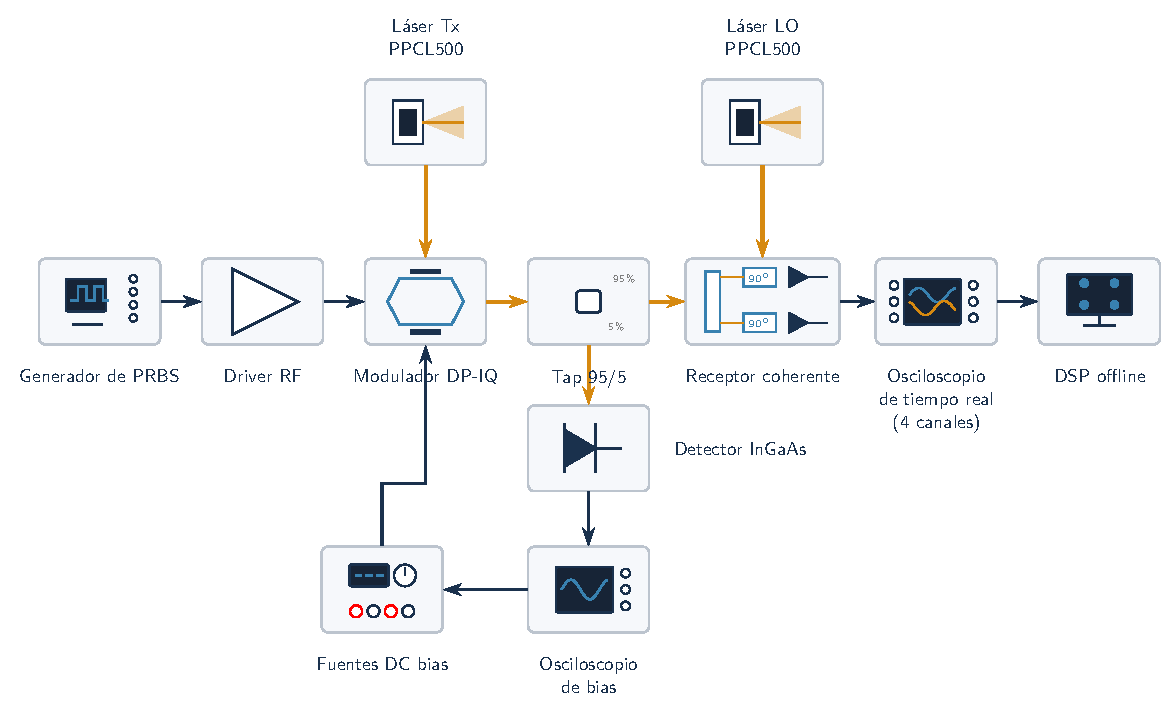
\includegraphics[width=\textwidth]{figuras/lab_setup_base.pdf}
  \caption[Esquema de medici\'on coherente DP-QPSK]{%
    Esquema de la configuraci\'on experimental. Los caminos \'opticos y
    el\'ectricos se indican en naranja y azul, respectivamente. La salida del
    \SI{5}{\percent} del acoplador \'optico se utiliza para alimentar el lazo
    de control del punto de polarizaci\'on (\emph{bias}) del modulador.}
  \label{fig:exp-setup}
\end{figure}

La \cref{fig:exp-setup} muestra el esquema completo de la configuraci\'on
experimental.

El generador de patrones produce cuatro secuencias PRBS independientes, una
para cada rama del modulador, correspondientes a las componentes en fase y
cuadratura de ambas polarizaciones. Un driver de RF de cuatro canales
amplifica estas se\~nales para alcanzar la excursi\'on de tensi\'on requerida
por el modulador. Como se explic\'o en la \cref{sec:trx-modulador}, cada
modulador Mach-Zehnder se polariza en el punto de m\'inima transmisi\'on. 

La portadora \'optica es generada por el l\'aser transmisor, un ITLA
sintonizable en la banda C, la cual ingresa al modulador de doble
polarizaci\'on. Dado que los puntos de operaci\'on de los moduladores no
permanecen constantes en el tiempo, sino que presentan derivas debido
principalmente a variaciones de temperatura y otras condiciones ambientales,
las seis tensiones de polarizaci\'on deben ajustarse din\'amicamente para
mantener las condiciones de operaci\'on deseadas. Para ello se dispone de un
lazo de control autom\'atico de bias. En concreto, a la salida del modulador
se dispone un tramo corto de fibra monomodo y un acoplador \'optico que divide
la potencia en dos ramas, del \SI{95}{\percent} y el \SI{5}{\percent}. La
primera se dirige hacia el receptor coherente, mientras que la segunda
alimenta un fotodetector de InGaAs. La se\~nal resultante es adquirida por un
osciloscopio y se utiliza como realimentaci\'on del algoritmo de control, que
ajusta las fuentes de tensi\'on continua para mantener los puntos de
operaci\'on del modulador.

Se utiliza otro l\'aser ITLA del mismo modelo que el transmisor como LO, que
se conecta directamente al receptor, es decir, el front-end \'optico. Dentro
se encuentra el par de h\'ibridos de \SI{90}{\degree} que baten la se\~nal contra el
oscilador local, y los cuatro pares de fotodiodos balanceados con sus
amplificadores de transimpedancia. El receptor genera as\'i cuatro tensiones,
que contienen la fase y cuadratura de cada polarizaci\'on.

El osciloscopio digitaliza estos cuatro canales. Por \'ultimo, las capturas se
guardan y se procesan despu\'es en MATLAB con la misma cadena de bloques del
cap\'itulo~\ref{cap:dsp}.

\begin{table}[htbp]
  \centering

  \begin{tabular}{lll}
    \toprule
    Funci\'on & Equipo & Caracter\'istica relevante \\
    \midrule
    Generador de patrones & Tektronix PPG3204      & cuatro canales, PRBS \\
    L\'aser Tx y LO       & Pure Photonics PPCL500 & sinton\'ia fina de $\pm\SI{30}{\giga\hertz}$ \\
    Front end coherente   & Lab Buddy DSC-R413     & h\'ibrido de \SI{90}{\degree} y balanceados \\
    Digitalizador         & Tektronix DPO70000SX   & \SI{50}{\giga S\per\second} por canal \\
    Control de bias       & Tektronix MDO3054      & lectura del detector del tap \\
    \bottomrule
  \end{tabular}
  \caption[Equipos utilizados en el laboratorio]{%
    Equipos utilizados y la caracter\'istica que importa en cada caso.}
  \label{tab:instrumental}
\end{table}


\section{Desempe\~no en t\'erminos de BER y EVM}
\label{sec:exp-tasas}
\label{sec:exp-osnr}

Se realizaron mediciones correspondientes a las tres tasas de transmisi\'on
consideradas, cambiando \'unicamente la frecuencia de reloj del generador y la
frecuencia de muestreo del osciloscopio. Las
\cref{fig:exp-const-125,fig:exp-const-25,fig:exp-const-32} muestran las
constelaciones recuperadas.

\begin{figure}[H]
  \centering
  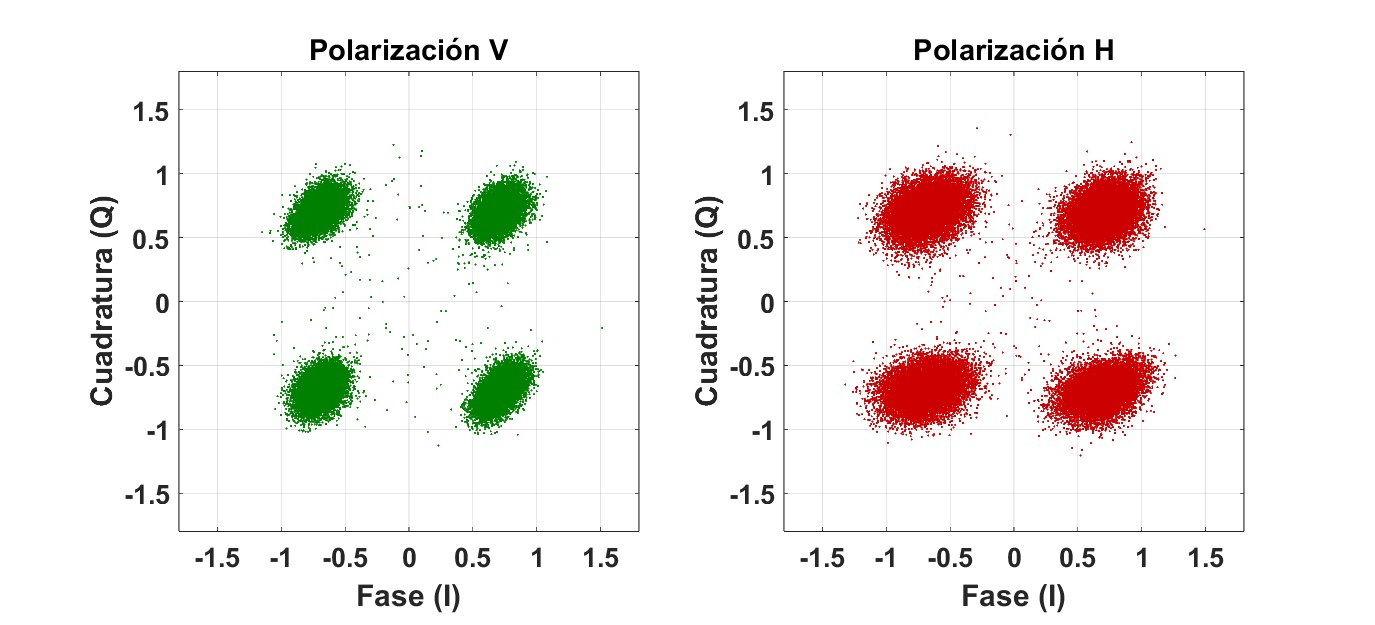
\includegraphics[width=0.95\textwidth]{figuras/Lab_12p5Gb_Final.jpg}
  \caption[Constelaci\'on medida a \SI{12.5}{\giga\baud}]{%
    Constelaci\'on recuperada de una captura de laboratorio a
    \SI{12.5}{\giga\baud}, equivalente a \SI{50}{\giga\bit\per\second}, con un
    EVM de \SI{16}{\percent}.}
  \label{fig:exp-const-125}
\end{figure}

\begin{figure}[H]
  \centering
  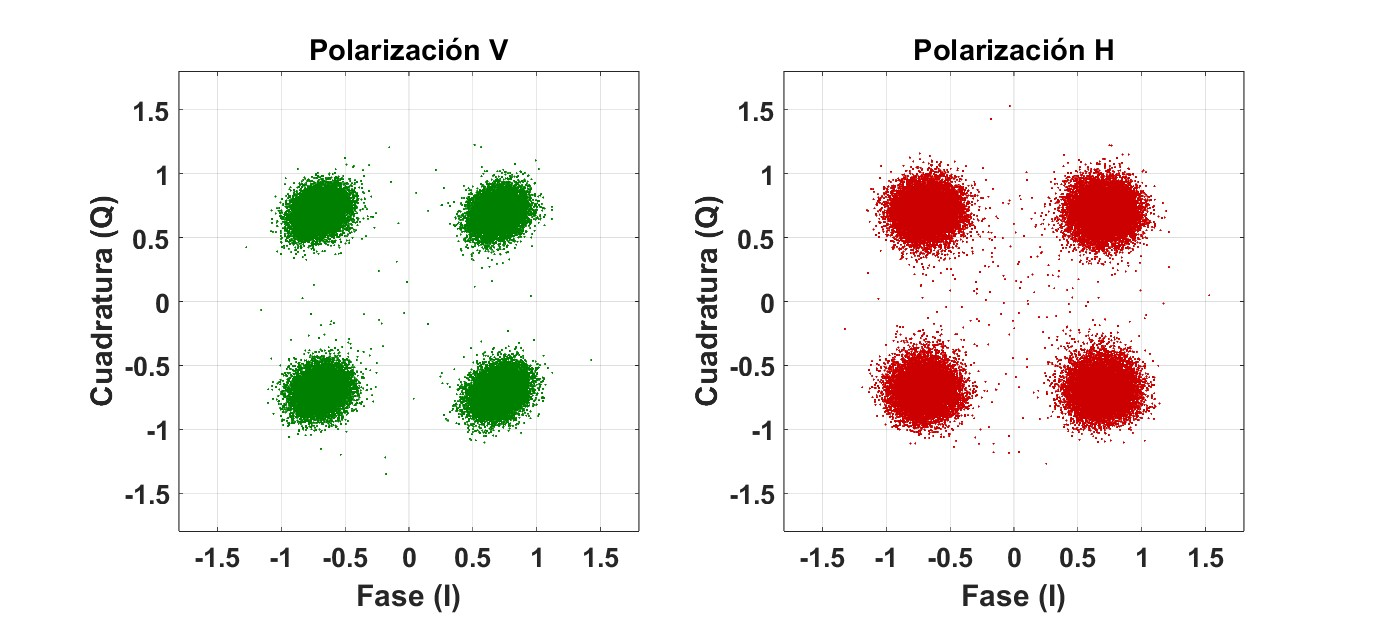
\includegraphics[width=0.95\textwidth]{figuras/Lab_25Gb_Final.jpg}
  \caption[Constelaci\'on medida a \SI{25}{\giga\baud}]{%
    Constelaci\'on recuperada a \SI{25}{\giga\baud}, equivalente a
    \SI{100}{\giga\bit\per\second}, con un EVM de \SI{22}{\percent}.}
  \label{fig:exp-const-25}
\end{figure}

\begin{figure}[H]
  \centering
  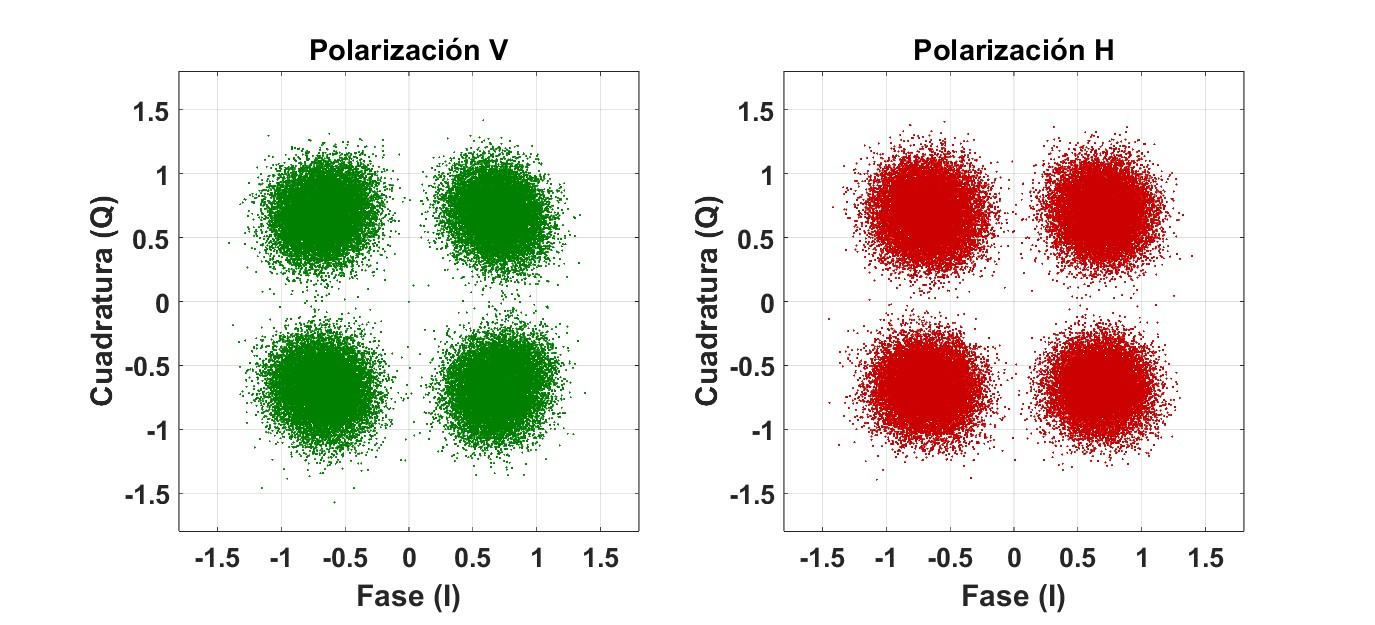
\includegraphics[width=0.95\textwidth]{figuras/Lab_32Gb_Final.jpg}
  \caption[Constelaci\'on medida a \SI{32}{\giga\baud}]{%
    Constelaci\'on recuperada a \SI{32}{\giga\baud}, equivalente a
    \SI{128}{\giga\bit\per\second}, que es la tasa de dise\~no del enlace, con
    un EVM de \SI{33}{\percent}.}
  \label{fig:exp-const-32}
\end{figure}

Se observan en los tres casos las constelaciones de QPSK y las dos
polarizaciones separadas. Por lo tanto, la cadena de procesamiento
demultiplexa, recupera el reloj, corrige el offset de frecuencia y engancha la
fase sobre se\~nales reales. Sin embargo, se observa que las nubes de
s\'imbolos no tienen la simetr\'ia circular propia de un canal AWGN. Esto
sugiere que hay cierto desbalance de cuadratura residual presente en
los s\'imbolos finales.

La diferencia entre las tres est\'a en el tama\~no de las nubes. A
\SI{12.5}{\giga\baud} los c\'umulos son compactos y quedan bien separados de
los ejes. A \SI{25}{\giga\baud} crecen de manera apreciable. A
\SI{32}{\giga\baud} el radio de cada nube es comparable a la distancia al eje,
y algunos s\'imbolos cruzan al cuadrante vecino, generando los primeros
errores contados.

En los experimentos de laboratorio no se dispuso de una medici\'on directa de
la OSNR. Por esta raz\'on se estim\'o una OSNR equivalente a partir de las
constelaciones recuperadas por el DSP, utilizando las relaciones del
\cref{cap:coherentes}. La magnitud del vector de error se relaciona con la relaci\'on
se\~nal-ruido mediante la \eqref{eq:evm-ber}, y la \eqref{eq:osnr-esno} la
refiere al ancho de banda de referencia de \SI{12.5}{\giga\hertz}.

Esta cifra es una OSNR equivalente y no una medici\'on \'optica. El EVM
incorpora tambi\'en degradaciones distintas del ruido \'optico, como el error
residual de ecualizaci\'on, el ruido de fase y las imperfecciones del
transmisor y del receptor. Por lo tanto, el valor estimado no coincide
necesariamente con la OSNR que se medir\'ia de forma directa con un analizador
de espectro \'optico.

\begin{table}[htbp]
  \centering

  \begin{tabular}{lccccc}
    \toprule
    Tasa & $\Rs$ & $\EVM$ & $E_s/N_0$ & $\OSNR$ equivalente & BER estimada \\
    \midrule
    \SI{50}{\giga\bit\per\second}  & \SI{12.5}{\giga\baud} & \SI{16}{\percent} & \SI{15.9}{\dB} & \SI{15.9}{\dB} & \num{2e-10} \\
    \SI{100}{\giga\bit\per\second} & \SI{25}{\giga\baud}   & \SI{22}{\percent} & \SI{13.2}{\dB} & \SI{16.2}{\dB} & \num{2.7e-6} \\
    \SI{128}{\giga\bit\per\second} & \SI{32}{\giga\baud}   & \SI{33}{\percent} & \SI{9.6}{\dB}  & \SI{13.7}{\dB} & \num{1.2e-3} \\
    \bottomrule
  \end{tabular}
  \caption[OSNR equivalente estimada en el banco]{%
    EVM medido en cada tasa, con la relaci\'on se\~nal-ruido y la OSNR
    equivalente que resultan. La columna $E_s/N_0$ es la relaci\'on
    el\'ectrica en el punto de decisi\'on.}
  \label{tab:exp-osnr}
\end{table}

En la \cref{tab:exp-osnr} se muestra la OSNR equivalente estimada para las
tasas de transmisi\'on consideradas. La potencia \'optica es la misma en las
tres medidas, ya que se us\'o la misma potencia de l\'aser, y la densidad
espectral de ruido tambi\'en, as\'i que al duplicar la tasa de s\'imbolo se
integra el doble de ruido y la relaci\'on cae \SI{3}{\dB}. Entre
\SI{12.5}{\giga\baud} y \SI{25}{\giga\baud} la ca\'ida medida es de
\SI{2.8}{\dB} contra \SI{3.0}{\dB} que predice la cuenta. Por lo tanto, la
transici\'on de \SI{50}{\giga\bit\per\second} a
\SI{100}{\giga\bit\per\second}, a estas potencias en el receptor, no degrada
nada que no sea directamente la penalidad por ancho de banda. En el tercer
experimento se analiza en mayor detalle. La OSNR equivalente, que no tiene en
cuenta este factor, queda pr\'acticamente igual en las dos tasas.

Por otro lado, el pasar de \SI{25}{\giga\baud} a \SI{32}{\giga\baud}
deber\'ia implicar \SI{1.1}{\dB} de relaci\'on se\~nal-ruido por ancho de banda y, sin embargo, se obtiene una diferencia de \SI{3.5}{\dB}. Hay por lo tanto \SI{2.4}{\dB} de exceso, y la OSNR equivalente cae de \SI{16.2}{\dB} a
\SI{13.7}{\dB}. Este exceso tiene tres contribuciones debidas al equipo
utilizado.

\paragraph{L\'imite de tasa de muestreo del osciloscopio}
El osciloscopio puede muestrear como m\'aximo a \SI{50}{\giga S\per\second}
por canal. A \SI{12.5}{\giga\baud} y \SI{25}{\giga\baud} esto alcanza para
capturar a dos muestras por s\'imbolo, que es la tasa a la que trabaja el DSP.
A \SI{32}{\giga\baud} se obtienen \num{1.5625} muestras por s\'imbolo y el DSP
tiene que interpolar hasta \num{2} antes de empezar. La
\cref{tab:sps-captura} resume la situaci\'on.

La interpolaci\'on aumenta la cantidad de muestras pero no agrega
informaci\'on. Con \SI{50}{\giga S\per\second} el l\'imite de Nyquist de la
captura queda en \SI{25}{\giga\hertz}, por debajo del contenido espectral que
la se\~nal NRZ a \SI{32}{\giga\baud} tiene por encima de esa frecuencia, de
modo que parte del espectro se pliega ya en la adquisici\'on. Lo que se pierde
en ese plegado no se recupera despu\'es en el procesamiento.

\begin{table}[htbp]
  \centering

  \begin{tabular}{lccc}
    \toprule
    Tasa & $\Rs$ & $F_s$ del osciloscopio & Muestras por s\'imbolo \\
    \midrule
    \SI{50}{\giga\bit\per\second}  & \SI{12.5}{\giga\baud} & \SI{25}{\giga S\per\second} & 2 \\
    \SI{100}{\giga\bit\per\second} & \SI{25}{\giga\baud}   & \SI{50}{\giga S\per\second} & 2 \\
    \SI{128}{\giga\bit\per\second} & \SI{32}{\giga\baud}   & \SI{50}{\giga S\per\second} & \num{1.5625} \\
    \bottomrule
  \end{tabular}
  \caption[Muestras por s\'imbolo en la captura]{%
    Frecuencia de muestreo y muestras por s\'imbolo disponibles en cada tasa.
    S\'olo la tasa de dise\~no queda por debajo de las dos muestras por
    s\'imbolo que necesita el DSP.}
  \label{tab:sps-captura}
\end{table}

\paragraph{El ancho de banda del camino el\'ectrico}
Los amplificadores de transimpedancia del front end y los drivers de
radiofrecuencia presentan una respuesta en frecuencia no plana, con una
atenuaci\'on creciente hacia las frecuencias m\'as altas del espectro de la
se\~nal. Esta limitaci\'on introduce distorsi\'on en la forma de los pulsos y
genera interferencia entre s\'imbolos, mucho m\'as nociva a
\SI{32}{\giga\baud} que a \SI{25}{\giga\baud} y \SI{12.5}{\giga\baud}. Si bien
el ecualizador adaptativo puede compensar parcialmente esta distorsi\'on, su
capacidad est\'a limitada por la amplificaci\'on del ruido que se produce al
intentar invertir la atenuaci\'on de las componentes espectrales de alta
frecuencia.

\paragraph{El skew entre ramas}
El cap\'itulo~\ref{cap:tolerancias} mostr\'o que el skew entre las ramas en
fase y cuadratura es el deterioro de margen m\'as estrecho de todo el
receptor, y que su efecto crece con la frecuencia. Ese retardo no proviene
\'unicamente del front end de recepci\'on, ya que el transmisor tambi\'en
introduce diferencias de camino entre las cuatro ramas. La tasa de
\SI{32}{\giga\baud} es la de mayor ancho de banda de las tres analizadas, de
modo que el mismo retardo f\'isico degrada m\'as la se\~nal.

Como conclusi\'on, se procesaron muestras a la tasa de dise\~no, con una OSNR
equivalente de \SI{13.7}{\dB}, un dec\'ibel por encima del umbral HD-FEC. Se
pudo recuperar la constelaci\'on QPSK en ambas polarizaciones.


\section{Barridos de potencia}
\label{sec:exp-barridos}

Las mediciones anteriores se realizaron para una \'unica condici\'on de
potencia \'optica recibida. En esta secci\'on se caracteriza el desempe\~no
del receptor en funci\'on de la potencia \'optica, con el objetivo de
determinar los niveles m\'inimos necesarios para su funcionamiento. Para ello
se realizaron dos barridos independientes, uno variando la potencia de la
se\~nal recibida y otro modificando la potencia del oscilador local.

Para realizar estas mediciones se introdujeron dos modificaciones en el
esquema experimental de la \cref{fig:exp-setup}. En primer lugar, se
reemplaz\'o el l\'aser transmisor por un ID Photonics CoBrite Tunable Laser
DX, que proporciona una mayor potencia \'optica de salida y permite ampliar el
rango de potencias evaluado. En segundo lugar, se incorpor\'o un atenuador
\'optico variable entre el acoplador 95/5 y el receptor coherente, para
controlar la potencia de se\~nal incidente sin modificar las condiciones de
operaci\'on del modulador. El esquema experimental resultante se presenta en
la \cref{fig:exp-setup-barrido}.

\begin{figure}[H]
  \centering
  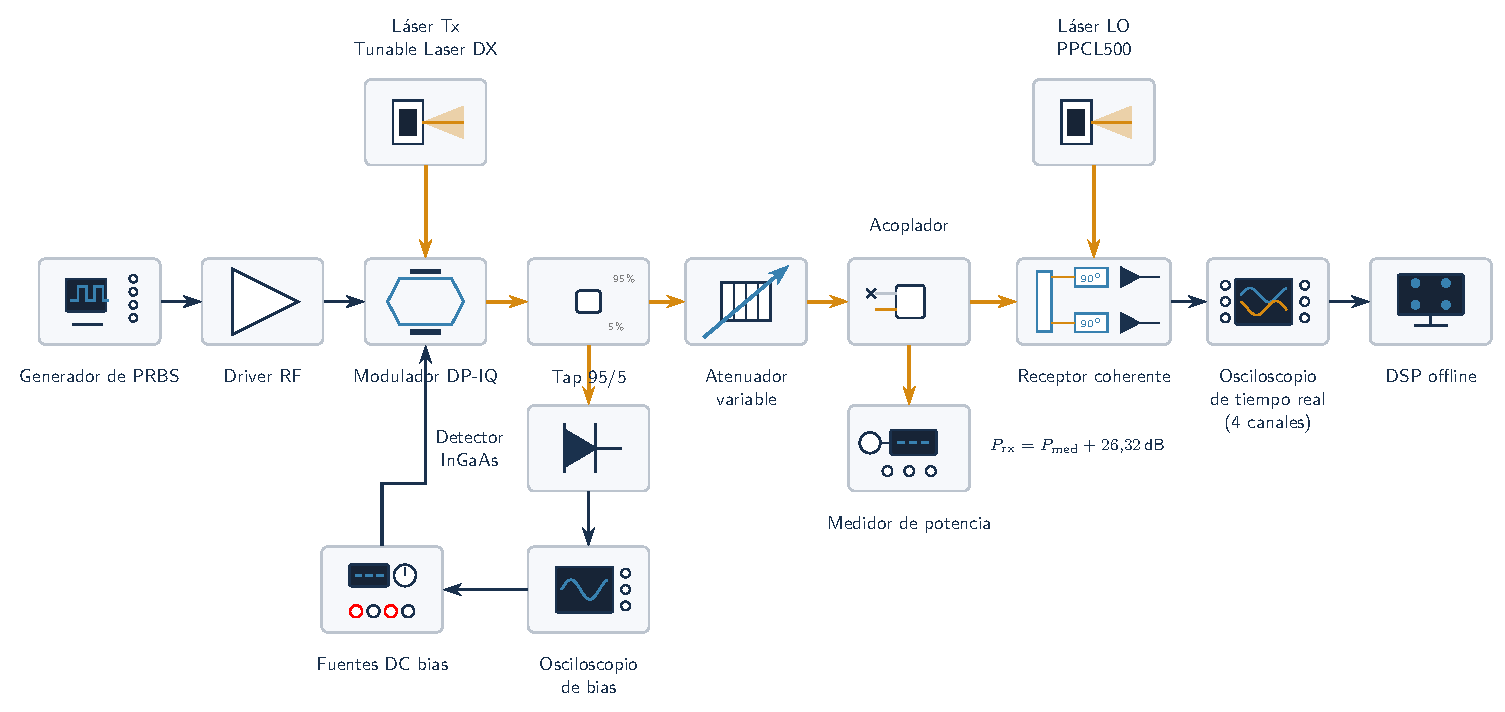
\includegraphics[width=\textwidth]{figuras/lab_setup_barrido.pdf}
  \caption[Esquema de medici\'on con atenuador variable]{%
    Esquema experimental utilizado para los barridos de potencia \'optica.
    Respecto de la configuraci\'on de la \cref{fig:exp-setup}, se incorpora un
    atenuador \'optico variable y un sistema de monitoreo compuesto por un
    acoplador \'optico y un medidor de potencia, que permite estimar la
    potencia \'optica incidente sobre el receptor.}
  \label{fig:exp-setup-barrido}
\end{figure}


Para estimar la potencia \'optica incidente sobre el receptor se incorpor\'o
un acoplador de fibra sintonizable, a modo de tap, ubicado despu\'es del
atenuador variable. Una de sus salidas se conecta al front end del receptor
coherente y la otra a un medidor de potencia \'optica. Se utiliz\'o una
relaci\'on de acoplamiento que permite dirigir la mayor parte de la potencia
hacia el receptor, manteniendo en la rama de monitoreo un nivel de potencia
suficiente para realizar una medici\'on confiable.

La diferencia de potencia entre ambas ramas se determin\'o mediante una
calibraci\'on experimental, obteni\'endose un valor de
$\Delta_{\mathrm{cal}} = \SI{26.3}{\dB}$. De esta manera, la potencia
\'optica incidente sobre el receptor puede calcularse a partir de la lectura
del medidor como
\begin{equation}
  P_{\mathrm{rx}} = P_{\mathrm{medidor}} + \Delta_{\mathrm{cal}},
  \label{eq:exp-calibracion}
\end{equation}
donde ambas potencias se expresan en \si{\dBm}. La calibraci\'on se
repiti\'o al inicio de cada sesi\'on de medici\'on y despu\'es de realizar
modificaciones en la cadena \'optica.

\subsection{Barrido de potencia de la se\~nal recibida}
\label{sec:exp-barrido-tx}

Manteniendo fija la potencia del oscilador local en su punto de trabajo
(\SI{8.0}{\dBm}), se reduce progresivamente la potencia \'optica de la
se\~nal recibida mediante el atenuador variable, en pasos de aproximadamente
\SI{0.5}{\dB}. En cada punto del barrido se realizan ocho capturas del
osciloscopio, que posteriormente se procesan con la cadena DSP del receptor.

Para cada nivel de potencia se obtienen dos estimaciones de la tasa de error
de bits. La primera se calcula por conteo directo, comparando la secuencia de
bits recuperada con la PRBS transmitida y acumulando los errores de las ocho
capturas. Dado que este m\'etodo tiene una resoluci\'on limitada por la
cantidad total de bits analizados, solo se representan los puntos con una
cantidad suficiente de errores para obtener una estimaci\'on confiable. La
segunda se obtiene a partir del EVM de la constelaci\'on recuperada,
siguiendo el procedimiento descrito en la \cref{sec:exp-osnr}. Ambos
resultados se presentan por separado para cada polarizaci\'on.

\begin{figure}[H]
  \centering
  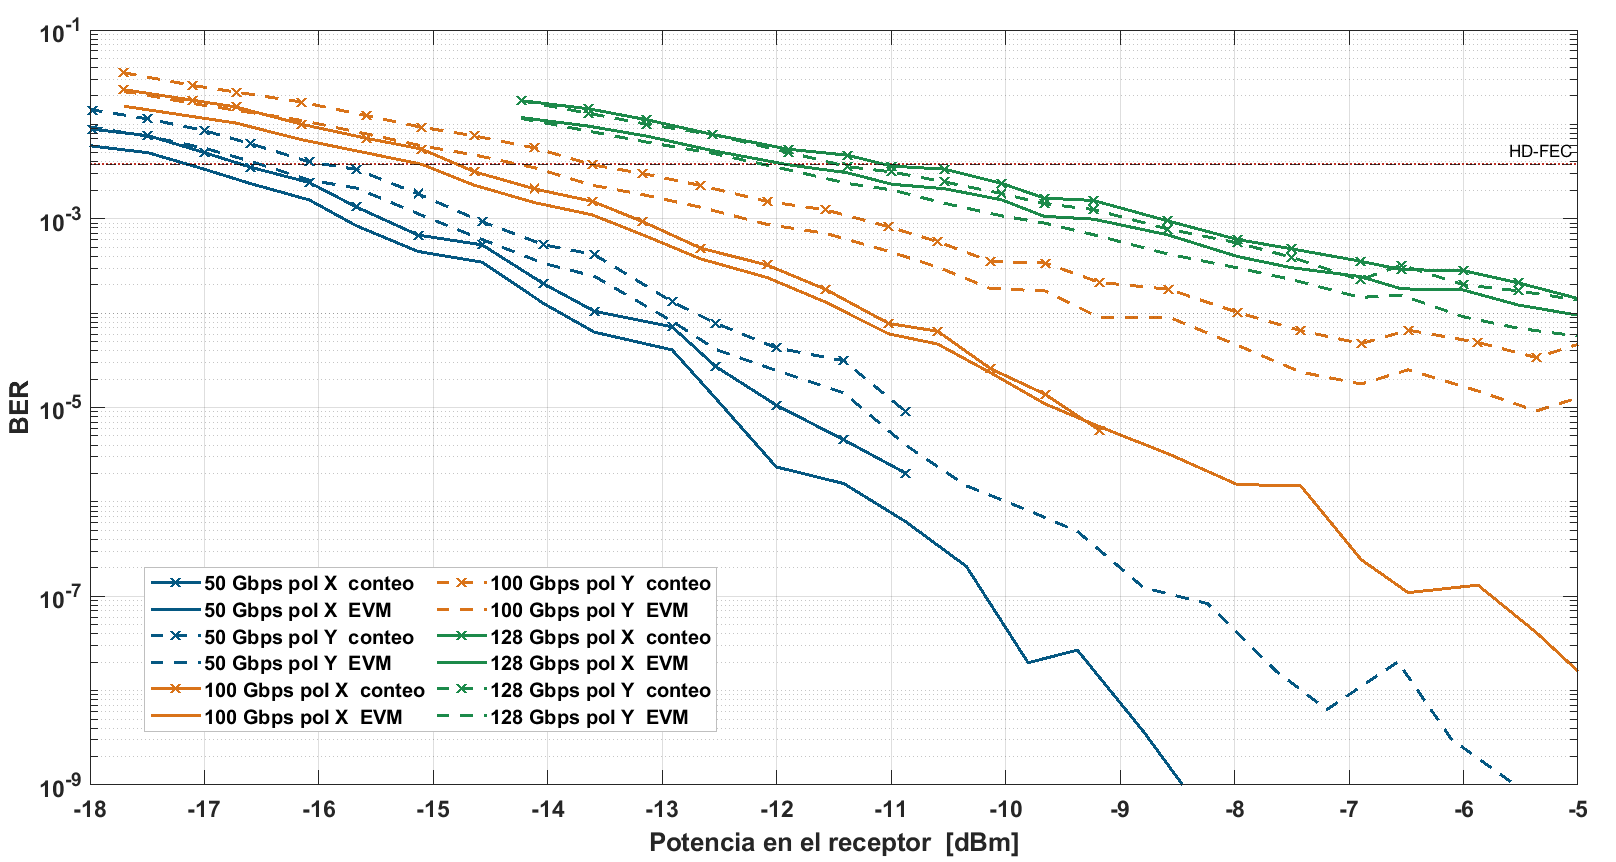
\includegraphics[width=\textwidth]{figuras/BarridoTxTodasLasTasas.png}
  \caption[Barrido de potencia de se\~nal en las tres tasas]{%
    BER en funci\'on de la potencia \'optica en el receptor para las tres
    tasas. El color indica la tasa, la l\'inea llena y la de trazos las
    polarizaciones X e Y, y las cruces la BER contada contra la estimada por
    EVM. La l\'inea punteada es el umbral HD-FEC.}
  \label{fig:exp-barrido-tx}
\end{figure}

La \cref{fig:exp-barrido-tx} muestra los resultados obtenidos para las tres
tasas de s\'imbolo, en un rango de potencia \'optica recibida de
\SIrange{-18}{-5}{\dBm}. Como era de esperar, el desempe\~no del receptor
mejora al aumentar la potencia de se\~nal. Tambi\'en se observa que una de las
polarizaciones presenta una BER sistem\'aticamente mayor en todo el rango
medido, lo que sugiere la existencia de diferencias en las caracter\'isticas
de los caminos de transmisi\'on o recepci\'on de ambas polarizaciones.

Tomando como referencia el cruce con el umbral HD-FEC de la BER medida por
conteo en la polarizaci\'on de peor desempe\~no, se obtiene una sensibilidad
de \SI{-16.0}{\dBm} a \SI{12.5}{\giga\baud}, \SI{-13.6}{\dBm} a
\SI{25}{\giga\baud} y \SI{-11.0}{\dBm} a \SI{32}{\giga\baud}. La diferencia
entre los dos primeros valores, de \SI{2.4}{\dB}, es cercana al incremento
te\'orico de \SI{3}{\dB} en la potencia requerida al duplicar la tasa de
s\'imbolo, manteniendo constante la relaci\'on se\~nal-ruido por s\'imbolo.
En cambio, el incremento de \SI{2.6}{\dB} observado al pasar de
\SI{25}{\giga\baud} a \SI{32}{\giga\baud} supera los \SI{1.1}{\dB} esperados
por el cambio de tasa. Esta diferencia es consistente con la penalidad
adicional observada a la tasa de dise\~no en la \cref{sec:exp-osnr}, que
ac\'a se manifiesta como un aumento de la potencia necesaria para alcanzar el
umbral de BER.

Por \'ultimo, la BER estimada a partir del EVM presenta una tendencia similar
a la BER medida por conteo, lo que respalda su utilidad como m\'etodo de
estimaci\'on indirecta.

La \cref{tab:exp-cruces-tx} resume las sensibilidades obtenidas para cada tasa
de s\'imbolo y polarizaci\'on.

% ---------------------------------------------------------------
\begin{table}[htbp]
  \centering

  \begin{tabular}{lccc}
    \toprule
    Tasa & Pol.\ X & Pol.\ Y & Diferencia \\
    \midrule
    \SI{50}{\giga\bit\per\second} & \SI{-16.68}{\dBm} & \SI{-15.97}{\dBm} & \SI{0.72}{\dB} \\
    \SI{100}{\giga\bit\per\second} & \SI{-14.80}{\dBm} & \SI{-13.63}{\dBm} & \SI{1.17}{\dB} \\
    \SI{128}{\giga\bit\per\second} & \SI{-11.52}{\dBm} & \SI{-11.03}{\dBm} & \SI{0.49}{\dB} \\
    \bottomrule
  \end{tabular}
  \caption[Cruce del umbral HD-FEC en el barrido de se\~nal]{%
    Potencia \'optica de se\~nal en el receptor a la que la BER contada de
    cada polarizaci\'on cruza el umbral HD-FEC, y diferencia entre las dos.}
  \label{tab:exp-cruces-tx}
\end{table}

\subsection{Barrido de potencia del oscilador local}
\label{sec:exp-barrido-lo}

En el segundo barrido se mantuvo fija la potencia \'optica de la se\~nal
recibida en \SI{-5.5}{\dBm} y se vari\'o la potencia del LO. Dado que el
l\'aser permite ajustar directamente su potencia de salida entre
\SIrange{7}{13}{\dBm}, las mediciones se realizaron en dos etapas. En la
primera, el LO se conect\'o directamente al receptor para cubrir el rango de
potencias m\'as altas. En la segunda, se incorpor\'o un atenuador fijo de
\SI{7.7}{\dB} a la salida del l\'aser para extender las mediciones hacia
potencias menores. De esta manera se cubri\'o un rango de
\SIrange{-0.3}{11}{\dBm} de potencia \'optica del LO incidente sobre el front
end. El procesamiento de las se\~nales y el c\'alculo de la BER se realizaron
siguiendo el mismo procedimiento que en el barrido anterior.

\begin{figure}[H]
  \centering
  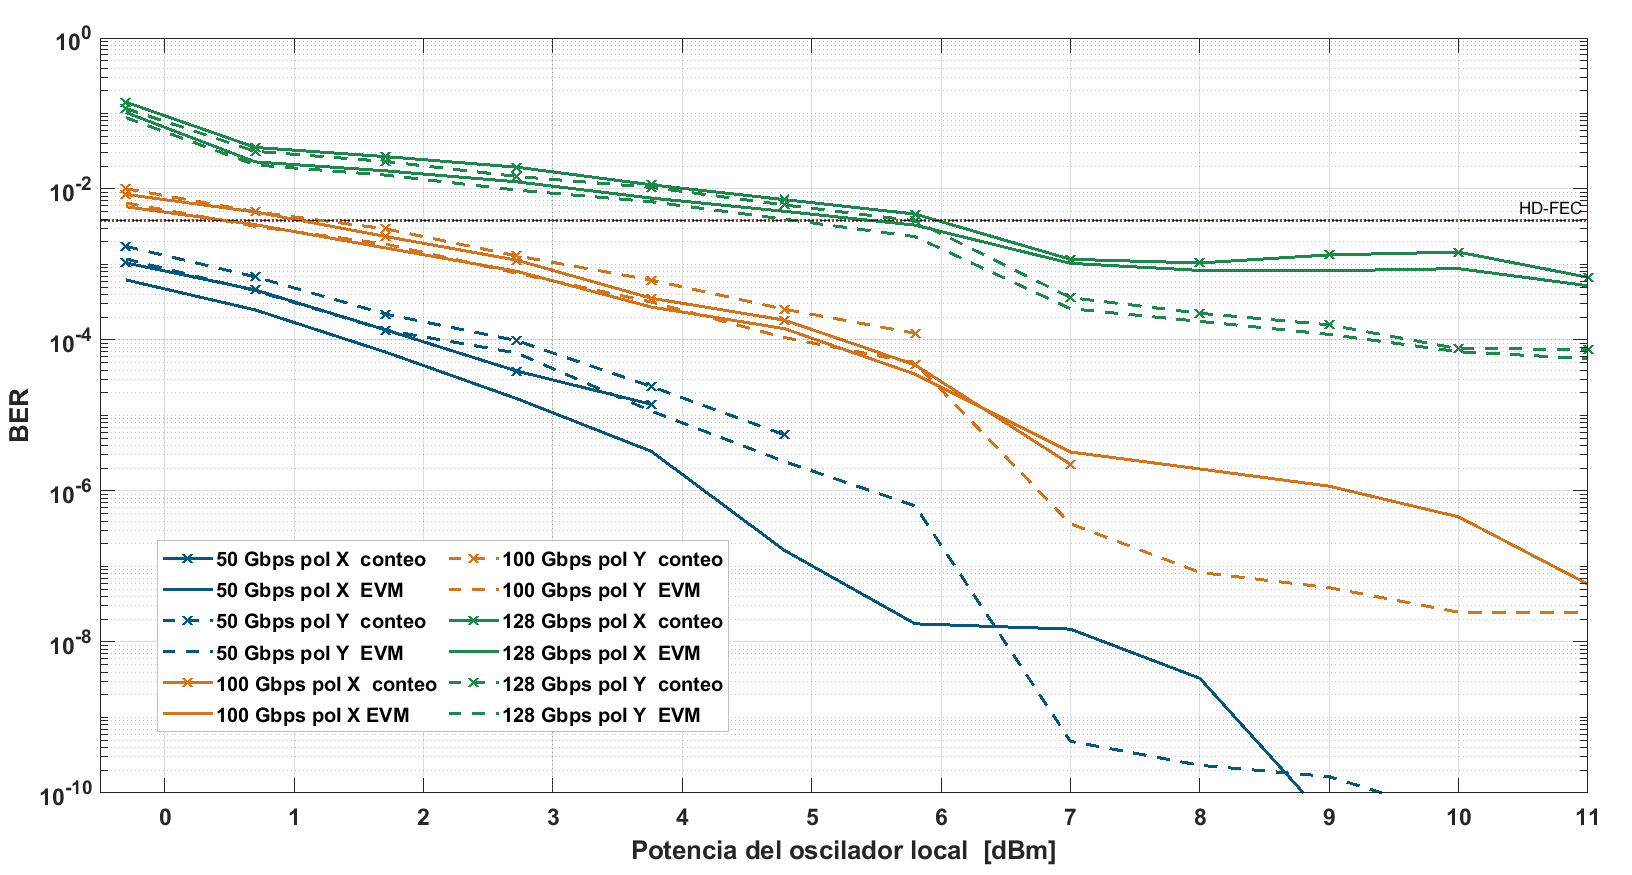
\includegraphics[width=\textwidth]{figuras/BarridoLOTodasLasTasas.png}
  \caption[Barrido de potencia de oscilador local en las tres tasas]{%
    BER en funci\'on de la potencia de oscilador local en el receptor para las
    tres tasas, con la potencia de se\~nal fija en \SI{-5.5}{\dBm}. La
    convenci\'on de colores, l\'ineas y marcadores es la misma que la de la
    \cref{fig:exp-barrido-tx}.}
  \label{fig:exp-barrido-lo}
\end{figure}

La \cref{fig:exp-barrido-lo} muestra los resultados obtenidos. Las curvas
presentan un comportamiento similar para las tres tasas de transmisi\'on. A
bajas potencias del LO, la BER disminuye r\'apidamente al aumentar su
potencia. A partir de aproximadamente \SI{7}{\dBm} la mejora se vuelve
considerablemente menor y, para \SI{128}{\giga\bit\per\second}, la BER
permanece pr\'acticamente constante entre \SI{7}{\dBm} y \SI{11}{\dBm}.

Este comportamiento es consistente con el esperado para un receptor coherente.
La amplitud de la corriente de batido es proporcional a la ra\'iz del producto
de las potencias \'opticas de la se\~nal y del oscilador local. Por lo tanto,
manteniendo fija la potencia de se\~nal, la potencia el\'ectrica de la se\~nal
detectada crece proporcionalmente con la potencia del LO. Mientras predomina
el ruido t\'ermico de la electr\'onica de recepci\'on, cuya potencia es
aproximadamente independiente del LO, cada incremento de \SI{1}{\dB} en su
potencia produce una mejora cercana a \SI{1}{\dB} en la relaci\'on
se\~nal-ruido el\'ectrica. Sin embargo, al aumentar la potencia del oscilador
local tambi\'en crece el ruido de disparo asociado a la fotocorriente, cuya
varianza es proporcional a la potencia \'optica recibida. Cuando este ruido
predomina, tanto la potencia el\'ectrica de se\~nal como la potencia de ruido
aumentan aproximadamente en la misma proporci\'on, por lo que la relaci\'on
se\~nal-ruido deja de mejorar de forma significativa.

El aplanamiento observado en las curvas indica que, a partir de cierta
potencia del LO, su incremento deja de producir una mejora apreciable en el
desempe\~no. En este r\'egimen la BER queda limitada por las restantes
contribuciones de ruido y distorsi\'on del sistema, incluyendo las
degradaciones identificadas en la \cref{sec:exp-osnr}.

A \SI{50}{\giga\bit\per\second} la BER permanece por debajo del umbral HD-FEC
en todo el rango medido. Para \SI{100}{\giga\bit\per\second} y
\SI{128}{\giga\bit\per\second}, los cruces con este umbral se producen a
potencias del LO de \SI{1.23}{\dBm} y \SI{5.98}{\dBm}, respectivamente,
tomando como referencia la BER medida por conteo en la polarizaci\'on de peor
desempe\~no.

La \cref{tab:exp-cruces-lo} resume las potencias m\'inimas del oscilador local
necesarias para alcanzar el umbral HD-FEC en cada tasa de transmisi\'on y
polarizaci\'on.

% ---------------------------------------------------------------
\begin{table}[htbp]
  \centering

  \begin{tabular}{lccc}
    \toprule
    Tasa & Pol.\ X & Pol.\ Y & Diferencia \\
    \midrule
    \SI{50}{\giga\bit\per\second}$^{*}$ & \SI{-1.45}{\dBm} & \SI{-1.04}{\dBm} & \SI{0.41}{\dB} \\
    \SI{100}{\giga\bit\per\second} & \SI{1.23}{\dBm} & \SI{0.60}{\dBm} & \SI{0.63}{\dB} \\
    \SI{128}{\giga\bit\per\second} & \SI{5.98}{\dBm} & \SI{6.19}{\dBm} & \SI{0.21}{\dB} \\
    \bottomrule
  \end{tabular}
  \caption[Cruce del umbral HD-FEC en el barrido de oscilador local]{%
    Potencia de oscilador local a la que la BER contada de cada
    polarizaci\'on cruza el umbral HD-FEC, y diferencia entre las dos. Como a
    \SI{50}{\giga\bit\per\second} el receptor nunca alcanza el umbral dentro
    del rango medido, los valores marcados con asterisco son una
    extrapolaci\'on sobre los cinco puntos m\'as bajos de potencia.}
  \label{tab:exp-cruces-lo}
\end{table}



\section{Efecto Doppler}
\label{sec:exp-doppler}

El tercer experimento consiste en un barrido del offset de frecuencia,
siguiendo el procedimiento de la \cref{sec:tol-doppler}. Para emular el
desplazamiento de frecuencia producido por el efecto Doppler en un enlace
LEO--GEO, se modific\'o la frecuencia \'optica del l\'aser transmisor mediante
comandos ITLA, con una resoluci\'on de \SI{1}{\mega\hertz} y un rango de
ajuste de $\pm\SI{30}{\giga\hertz}$.

Para cada tasa de s\'imbolo, el barrido se realiz\'o desde un offset nulo
hasta \SI{1}{\giga\hertz} por encima del l\'imite te\'orico de estimaci\'on de
$\Rs/4$, utilizando pasos de \SI{500}{\mega\hertz}. Se realizaron tres pasadas
por cada punto para considerar las posibles variaciones temporales de la
frecuencia de emisi\'on de los l\'aseres. Las se\~nales adquiridas se
procesaron posteriormente con la misma cadena DSP utilizada en las mediciones
del punto de trabajo.

\begin{figure}[H]
  \centering
  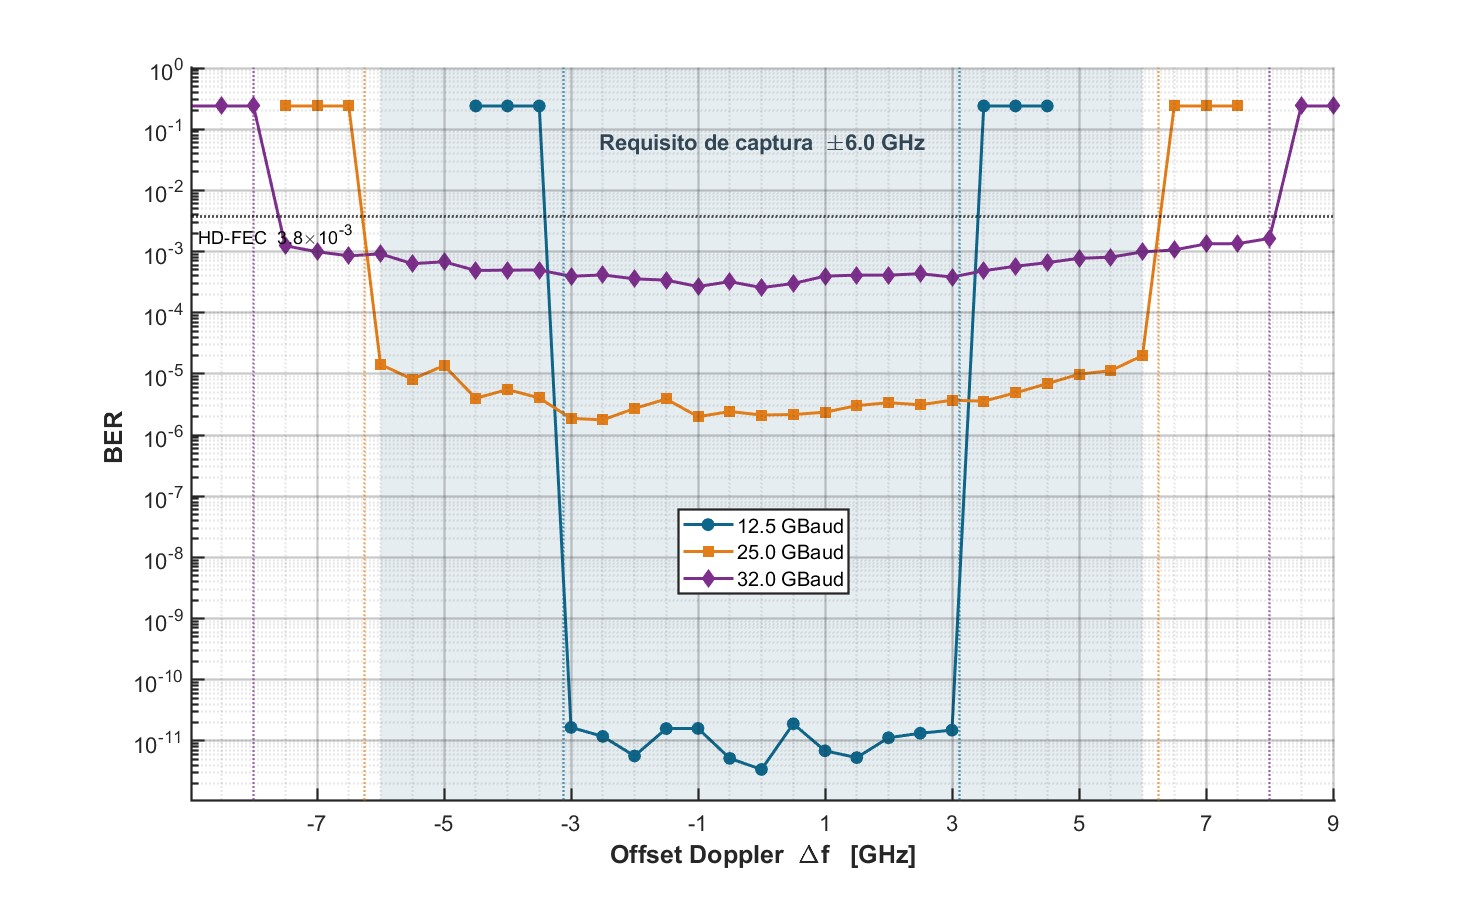
\includegraphics[width=0.92\textwidth]{figuras/DopplerComparacionExperimentalFinal.jpg}
  \caption[Barrido de offset Doppler medido en el laboratorio]{%
    BER estimada a partir del EVM contra offset de frecuencia medido en el
    laboratorio para las tres tasas, con tres pasadas por punto y paso de
    \SI{500}{\mega\hertz}. El piso de BER sube con la tasa por lo discutido en
    la \cref{sec:exp-osnr}.}
  \label{fig:exp-doppler}
\end{figure}

La \cref{fig:exp-doppler} muestra los resultados obtenidos. Las tres tasas
presentan un comportamiento similar. La BER estimada se mantiene
aproximadamente constante dentro del rango de funcionamiento del estimador de
frecuencia y aumenta abruptamente al superar su l\'imite de captura. En este
\'ultimo r\'egimen la estimaci\'on alcanza valores cercanos a \num{0.24},
correspondientes a un EVM de aproximadamente \SI{141}{\percent} al aplicar la
relaci\'on te\'orica utilizada para QPSK. Este incremento no representa
necesariamente una degradaci\'on progresiva de la calidad de la se\~nal, sino
que indica que el estimador de frecuencia deja de compensar correctamente el
offset, tal como se observ\'o en las simulaciones. Tambi\'en se aprecia un
ligero aumento de la BER dentro del rango de captura, a medida que crece el
valor absoluto del offset. Este comportamiento se analiza en la siguiente
secci\'on y se compara con los resultados de simulaci\'on.


\subsection{Espectro con y sin offset}
\label{sec:exp-doppler-espectro}

El efecto del offset sobre la se\~nal se ve directamente en el espectro de la
captura. La \cref{fig:exp-doppler-espectro-lab} compara dos medidas a
\SI{32}{\giga\baud}, una centrada y otra con un offset de
\SI{7}{\giga\hertz}.

\begin{figure}[H]
  \centering
  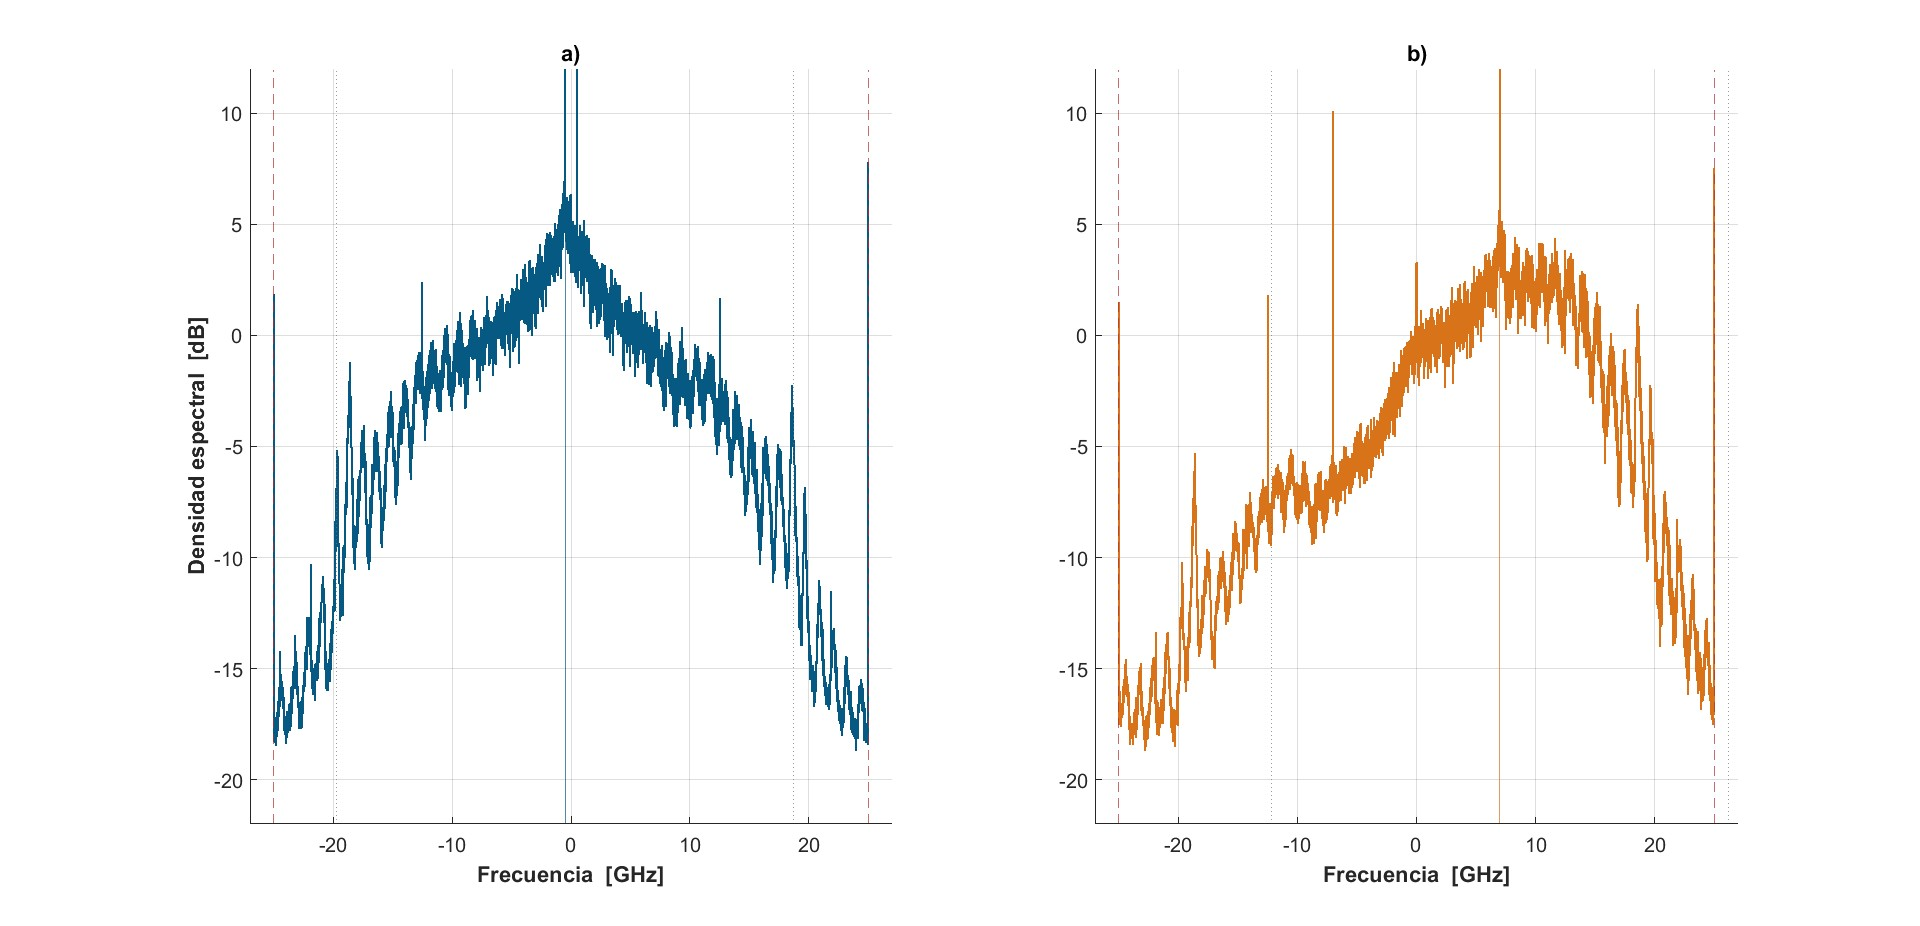
\includegraphics[width=\textwidth]{figuras/EspectroParaDistintosBW_LAB.jpg}
  \caption[Espectro medido con y sin offset Doppler]{%
    Densidad espectral de la se\~nal capturada a \SI{32}{\giga\baud}, a) sin
    offset y b) con un offset de \SI{7}{\giga\hertz}. Las l\'ineas de trazos
    marcan los \SI{\pm 25}{\giga\hertz} de Nyquist del osciloscopio.}
  \label{fig:exp-doppler-espectro-lab}
\end{figure}

Sin offset, el espectro de la se\~nal se encuentra centrado en continua y
presenta una distribuci\'on aproximadamente sim\'etrica respecto del origen.
Al introducir un offset, el espectro se desplaza en frecuencia. Debido a la
respuesta pasabajos del front end y del sistema de adquisici\'on, las
componentes desplazadas hacia frecuencias m\'as altas experimentan una mayor
atenuaci\'on, lo que introduce una distorsi\'on espectral asim\'etrica. A
\SI{32}{\giga\baud}, con un offset de \SI{7}{\giga\hertz}, parte del contenido
espectral de la se\~nal puede incluso superar el l\'imite de Nyquist del
osciloscopio, situado en \SI{25}{\giga\hertz}. Tambi\'en se observa el
desplazamiento de una componente residual de portadora, que permite
identificar visualmente el offset aplicado.

\begin{figure}[H]
  \centering
  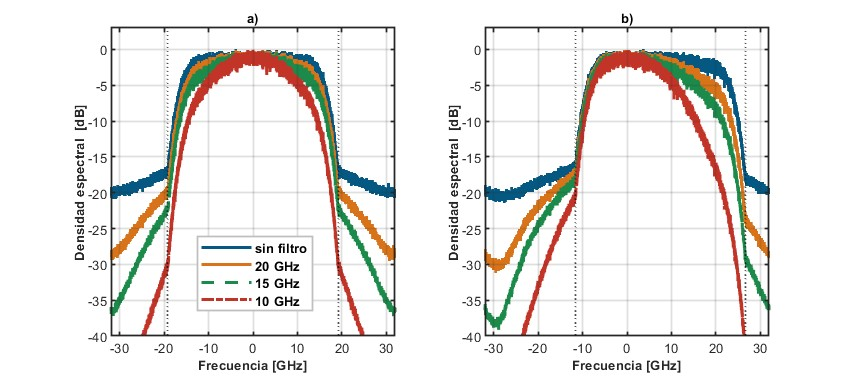
\includegraphics[width=\textwidth]{figuras/EspectroParaDistintosBWFotodiodos.jpg}
  \caption[Espectro simulado con y sin offset Doppler]{%
    Densidad espectral en simulaci\'on a \SI{32}{\giga\baud}, a) sin offset y
    b) con \SI{7}{\giga\hertz} de offset, para distintos anchos de banda. Las
    l\'ineas punteadas son los bordes de la banda de la se\~nal.}
  \label{fig:exp-doppler-espectro-sim}
\end{figure}

La \cref{fig:exp-doppler-espectro-sim} reproduce esta comparaci\'on mediante
simulaci\'on, considerando distintos anchos de banda para el filtro del
receptor. Mientras que la simulaci\'on utiliza pulsos conformados mediante un
filtro RRC, en el laboratorio se emplean se\~nales NRZ, por lo que sus
distribuciones espectrales son diferentes. Sin embargo, en ambos casos se
observa que el offset desplaza el espectro respecto de la respuesta en
frecuencia del receptor, produciendo una atenuaci\'on asim\'etrica que se
acent\'ua al reducir el ancho de banda. Este efecto contribuye a explicar el
aumento gradual de la BER observado dentro del rango de captura del estimador
de frecuencia, que se analiza con mayor detalle en la
\cref{sec:exp-comparacion}.




\section{Comparaci\'on con la simulaci\'on}
\label{sec:exp-comparacion}


\subsection{Constelaciones}

Las \cref{fig:exp-comp-125,fig:exp-comp-25,fig:exp-comp-32} son las
constelaciones que produce la simulaci\'on en las mismas tres tasas.

\begin{figure}[H]
  \centering
  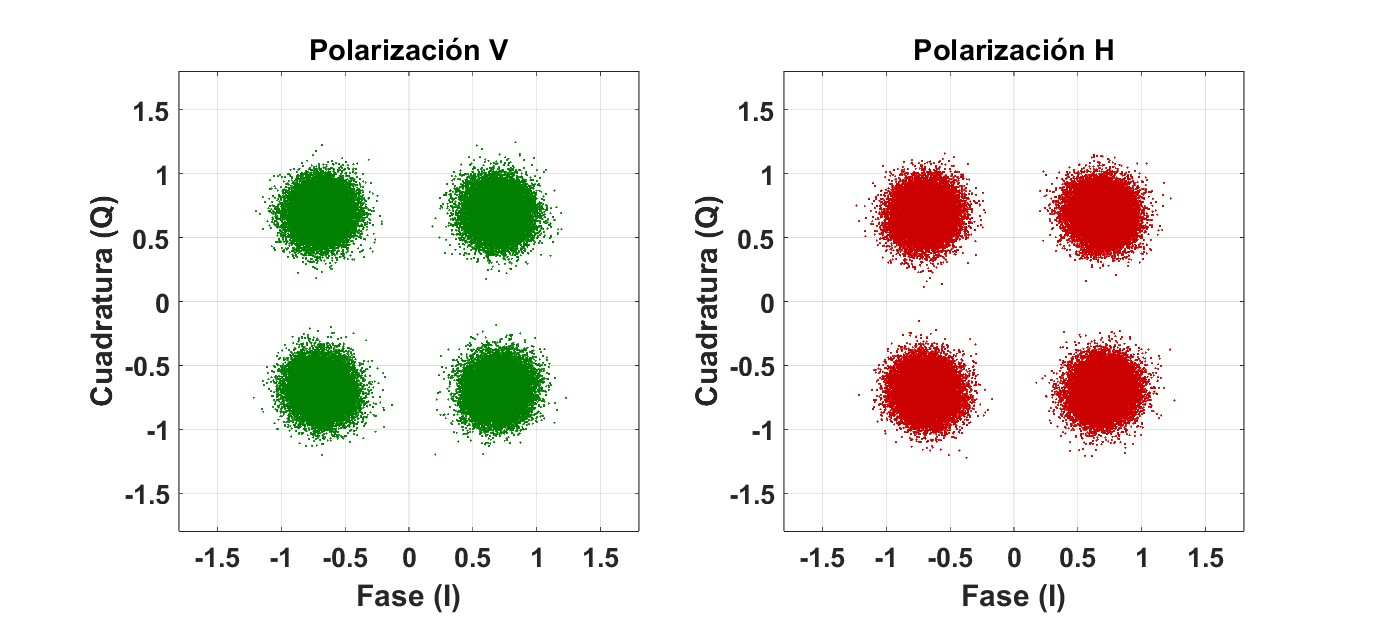
\includegraphics[width=0.95\textwidth]{figuras/Pol2_12p5Gb_Final.jpg}
  \caption[Constelaci\'on simulada a \SI{12.5}{\giga\baud}]{%
    Constelaci\'on de simulaci\'on a \SI{12.5}{\giga\baud}, para comparar con
    la \cref{fig:exp-const-125}.}
  \label{fig:exp-comp-125}
\end{figure}

\begin{figure}[H]
  \centering
  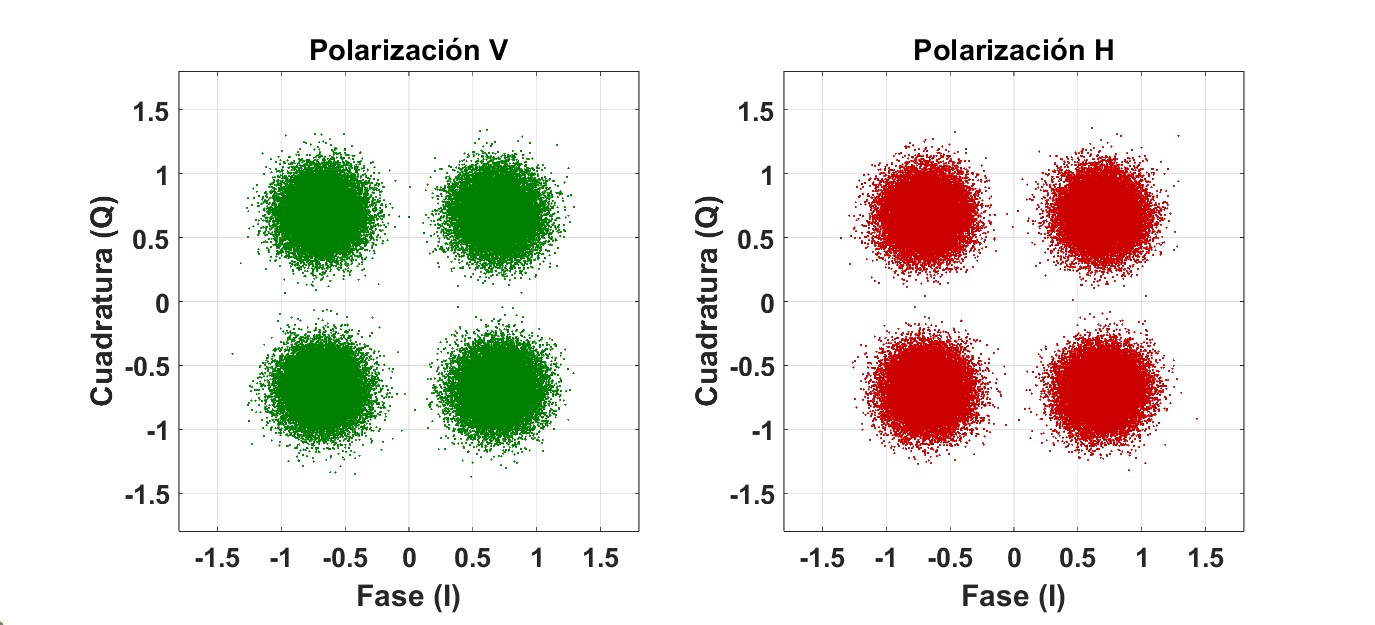
\includegraphics[width=0.95\textwidth]{figuras/Pol2_25Gb_Final.jpg}
  \caption[Constelaci\'on simulada a \SI{25}{\giga\baud}]{%
    Constelaci\'on de simulaci\'on a \SI{25}{\giga\baud}, para comparar con
    la \cref{fig:exp-const-25}.}
  \label{fig:exp-comp-25}
\end{figure}

\begin{figure}[H]
  \centering
  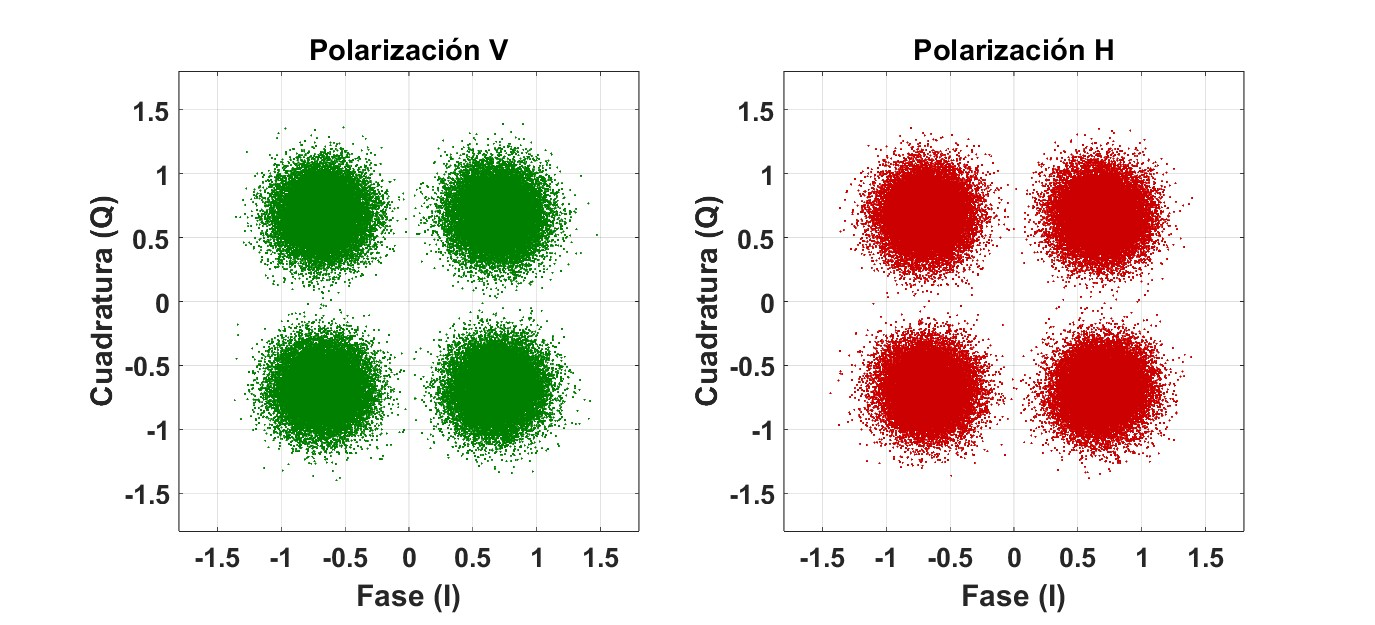
\includegraphics[width=0.95\textwidth]{figuras/Pol2_32Gb_Final.jpg}
  \caption[Constelaci\'on simulada a \SI{32}{\giga\baud}]{%
    Constelaci\'on de simulaci\'on a \SI{32}{\giga\baud}, para comparar con
    la \cref{fig:exp-const-32}.}
  \label{fig:exp-comp-32}
\end{figure}

La simulaci\'on se corri\'o al nivel de ruido que reproduce el EVM medido en cada
tasa, de modo que el tama\~no de las nubes no es una predicci\'on
independiente sino un ajuste. 
Compar\'andolas con las constelaciones obtenidas en el laboratorio, las
nubes simuladas son redondas y est\'an centradas en los mismos puntos, sin
rotaci\'on residual, sin elongaci\'on en una direcci\'on y sin sesgo entre las
dos polarizaciones. En cambio, las constelaciones finales del laboratorio parecen tener un 
desbalance de cuadratura que el GSOP no pudo compensar completamente.


\subsection{Tolerancia al offset Doppler}

Se reutiliza el gr\'afico del barrido de
offset simulado de la \cref{sec:tol-doppler} (\cref{fig:exp-doppler-sim}), con las mismas tres tasas que
la \cref{fig:exp-doppler}.

\begin{figure}[H]
  \centering
  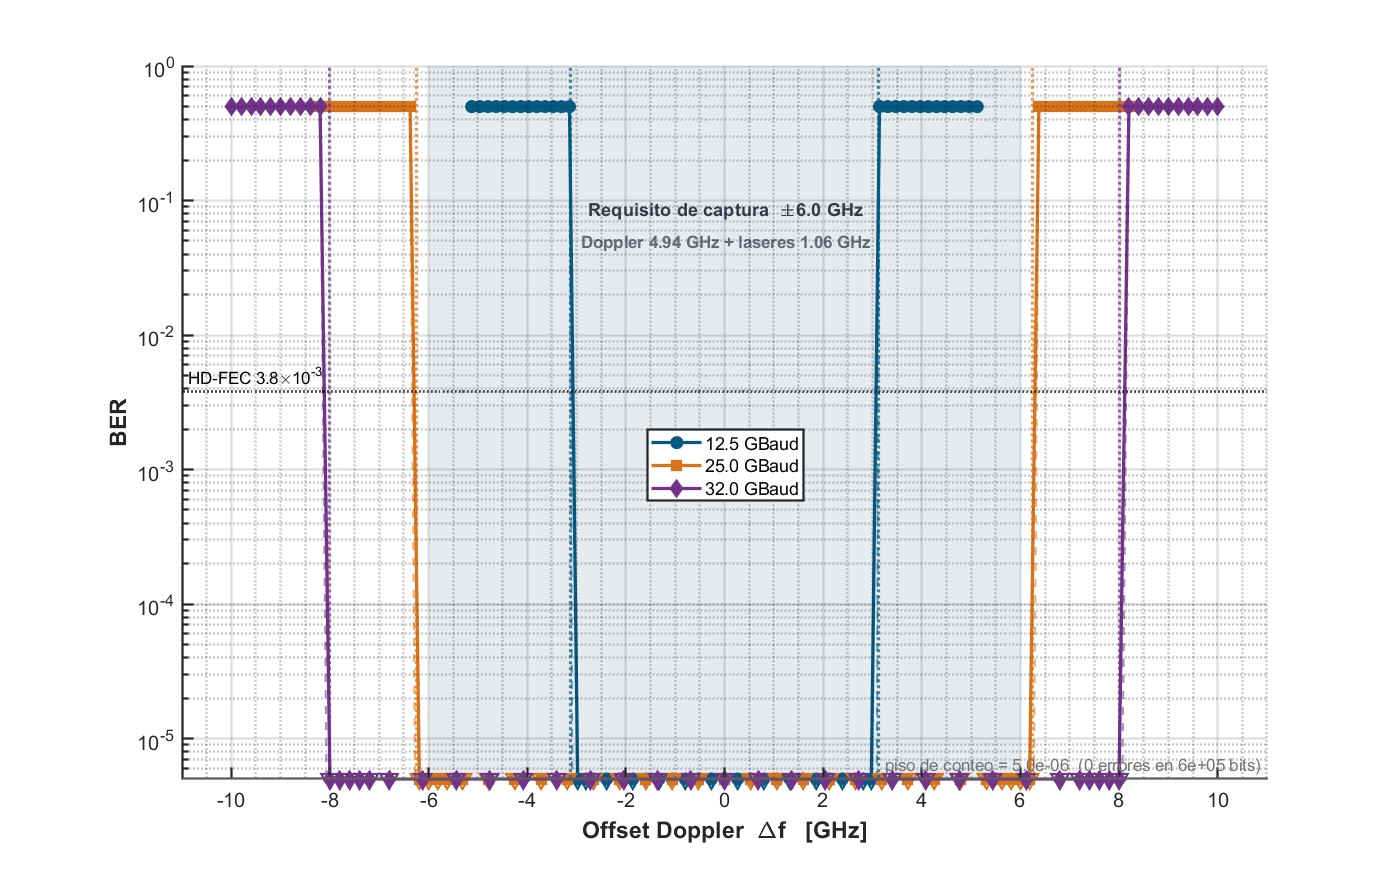
\includegraphics[width=0.92\textwidth]{figuras/EfectoDopplerFiguraFinalSimulacion.jpg}
  \caption[Barrido de offset Doppler en simulaci\'on]{%
    BER contra offset Doppler en simulaci\'on para las tres tasas de s\'imbolo,
    a OSNR fija. Es la misma figura de la \cref{fig:tol-doppler-sim},
    reproducida para comparar con la \cref{fig:exp-doppler}. La franja
    sombreada es el requisito de captura del enlace, \SI{\pm 6.0}{\giga\hertz},
    y la l\'inea de trazos el umbral HD-FEC.}
  \label{fig:exp-doppler-sim}
\end{figure}

La \cref{tab:exp-doppler} muestra el punto de corte medido contra el simulado
y contra el l\'imite te\'orico $\Rs/4$.

\begin{table}[htbp]
  \centering

  \begin{tabular}{lcccc}
    \toprule
    Tasa & $\Rs/4$ & Simulaci\'on & Laboratorio & Diferencia \\
    \midrule
    \SI{12.5}{\giga\baud} & \SI{3.125}{\giga\hertz} & \num{\pm 3.1}  & \num{\pm 3.0} & \SI{100}{\mega\hertz} \\
    \SI{25}{\giga\baud}   & \SI{6.25}{\giga\hertz}  & \num{\pm 6.25} & \num{\pm 6.0} & \SI{250}{\mega\hertz} \\
    \SI{32}{\giga\baud}   & \SI{8.0}{\giga\hertz}   & \num{\pm 8.0}  & $+8{,}0\,/\,-7{,}5$ & \SIrange{0}{500}{\mega\hertz} \\
    \bottomrule
  \end{tabular}
  \caption[Ventana de captura medida contra simulada]{%
    Offset de frecuencia donde el receptor falla, en laboratorio y en
    simulaci\'on, contra el l\'imite te\'orico $\Rs/4$.}
  \label{tab:exp-doppler}
\end{table}

Las tres tasas coinciden dentro de un paso de grilla, y fallan en
$\Rs/4$. En el laboratorio, el quiebre se presenta sistem\'aticamente un poco antes debido al paso de frecuencia entre mediciones. A su vez, existe un residuo de frecuencia entre los dos
l\'aseres de \SIrange{40}{95}{\mega\hertz} que puede correr
el punto de quiebre efectivo, lo que puede explicar la falla asim\'etrica en \SI{32}{\giga\baud}.



Dentro del rango enganchado hay una segunda diferencia. En el laboratorio
la BER aumenta ligeramente con el valor absoluto del offset, pero la simulaci\'on
no muestra esta pendiente. En el barrido contra la familia de OSNR de la
\cref{sec:tol-doppler-osnr}, a \SI{32}{\giga\baud} y \SI{16}{\dB}, el EVM
simulado pasa de \SI{26.57}{\percent} en \SI{0.2}{\giga\hertz} a
\SI{26.58}{\percent} en \SI{7.8}{\giga\hertz}, as\'i que la pendiente no
viene del procesamiento sino de los equipos. Adem\'as se observa que esta degradaci\'on crece con la tasa. A
\SI{12.5}{\giga\baud} casi no se aprecia, mientras que a \num{25} y
\SI{32}{\giga\baud}, la BER aumenta relativamente m\'as, lo que sugiere que el 
ancho de banda del receptor ocasiona el fen\'omeno. El offset desplaza el espectro de la se\~nal hacia uno de
los bordes de la banda del front-end y del osciloscopio, que est\'an
centradas en continua, y a \SI{32}{\giga\baud} el borde de la se\~nal llega a
los \SI{25}{\giga\hertz} de Nyquist del osciloscopio, que muestrea a
\SI{50}{\giga S\per\second}. En la simulaci\'on, en cambio, se utilizaron los anchos de banda
de las hojas de datos de los equipos, que resultaron ser m\'as grandes que los reales. En estas condiciones, y para 
los valores de Doppler que se manejan en el enlace,
el ancho de banda no es un limitante.


Para comprobarlo se repiti\'o el barrido de offset en simulaci\'on variando el
ancho de banda del receptor. La \cref{fig:exp-doppler-bw}
muestra el EVM resultante a la tasa de dise\~no.

\begin{figure}[H]
  \centering
  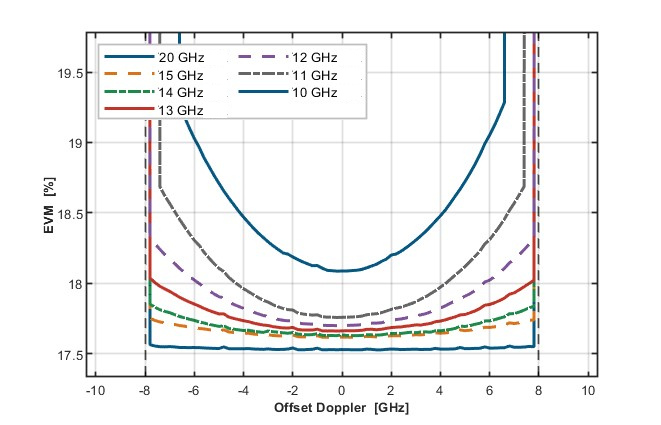
\includegraphics[width=0.8\textwidth]{figuras/BarridoOffsetDistintosBW.jpg}
  \caption[Barrido de offset Doppler para distintos anchos de banda]{%
    EVM contra offset Doppler en simulaci\'on a \SI{32}{\giga\baud}, para
    anchos de banda de receptor de \SIrange{10}{20}{\giga\hertz}. Las
    lineas verticales en $\pm\SI{8}{\giga\hertz}$ son el l\'imite de captura
    $\Rs/4$.}
  \label{fig:exp-doppler-bw}
\end{figure}

Con \SI{20}{\giga\hertz} de ancho de banda la curva es plana en todo el rango
enganchado, que es el caso de la \cref{fig:exp-doppler-sim}. Al achicar el
filtro el EVM sube en todo el barrido y, sobre todo, se curva. Con
\SI{10}{\giga\hertz} pasa de \SI{18.1}{\percent} en el centro a m\'as de
\SI{19}{\percent} en $\pm\SI{6.5}{\giga\hertz}$. Tambi\'en se observa que, por debajo de cierto valor
de ancho de banda, el rango \'util de captura disminuye, indicando que la señal qued\'o
filtrada por el receptor y el DSP no puede compensar la distorsi\'on.

El modelo reproduce entonces la pendiente medida en cuanto se le pone un ancho
de banda comparable al del laboratorio, lo que confirma que la
pendiente viene del equipo utilizado y no del procesamiento.


\section{Conclusiones}
\label{sec:exp-conclusiones}

El procesamiento recupera la constelaci\'on sobre se\~nales reales en las tres
tasas medidas, incluida la tasa de dise\~no de
\SI{128}{\giga\bit\per\second}, sin ninguna modificaci\'on respecto de la
versi\'on validada en simulaci\'on.

Los barridos de potencia dan la sensibilidad del conjunto. Sobre la BER
contada de la peor polarizaci\'on, el umbral HD-FEC se cruza con
\SI{-16.0}{\dBm} de se\~nal a \SI{12.5}{\giga\baud}, \SI{-13.6}{\dBm} a
\SI{25}{\giga\baud} y \SI{-11.0}{\dBm} a \SI{32}{\giga\baud}, los tres dentro
del rango de entrada que especifica el receptor. El primer escal\'on es del
orden de los \SI{3}{\dB} que cuesta duplicar la tasa de s\'imbolo y el segundo
vuelve a mostrar el exceso de la tasa de dise\~no que ya hab\'ia aparecido en
el punto de trabajo. Del lado del oscilador local el comportamiento es el de
un receptor coherente: por debajo de unos \SI{7}{\dBm} cada dec\'ibel se
traduce en un dec\'ibel de relaci\'on se\~nal-ruido, y por encima las curvas
se aplanan, de modo que llevar el oscilador al extremo alto de su rango no
agrega margen.


La tolerancia al offset Doppler medida en el laboratorio reproduce la simulada
en las tres tasas, confirmando el
l\'imite te\'orico de $\Rs/4$. Del lado del requisito, el resultado es el mismo
que en simulaci\'on. Utilizar una tasa de \SI{12.5}{\giga\baud} no cubre los
$\pm\SI{6.0}{\giga\hertz}$ del enlace, \SI{25}{\giga\baud} los cubre
justo, y \SI{32}{\giga\baud} los cubre con margen.

El ancho de banda el\'ectrico del camino de recepci\'on aparece como un segundo
efecto, separado del l\'imite de captura. Dentro del rango enganchado la BER
medida crece con el valor absoluto del offset, y la simulaci\'on reproduce esta
pendiente cuando se disminuye el ancho de banda del front end, de modo que viene del equipo
del laboratorio y no del procesamiento. Con los anchos de banda de las hojas de
datos la curva es plana, as\'i que para el rango de Doppler del enlace el
ancho de banda no es un limitante.


La limitaci\'on del laboratorio est\'a en el equipo utilizado, no en el receptor. La
frecuencia de muestreo del osciloscopio impide capturar la tasa de dise\~no
a dos muestras por s\'imbolo. 
Por \'ultimo, una comparaci\'on m\'as objetiva entre desempeños en el laboratorio 
y en la simulaci\'on ser\'ia posible midiendo OSNR directamente y no estim\'andola. Trazar la curva de BER contra OSNR, y compararla
contra la del cap\'itulo~\ref{cap:enlace}, es la continuaci\'on natural de
este trabajo.

% !TeX root = ../main.tex
%% =======================================================================
%  CAPITULO 9 — CONCLUSIONES

\chapter{Conclusiones}
\label{cap:conclusiones}

El receptor DP-QPSK de \SI{128}{\giga\bit\per\second} desarrollado en este
trabajo compensa el offset Doppler y su deriva, la rotaci\'on del estado de
polarizaci\'on y el ruido de los l\'aseres del enlace LEO--GEO. Frente a cada
uno de esos deterioros del canal queda margen sobre el valor f\'isico. Tambi\'en
se desarroll\'o el balance de potencias, llegando a la conclusi\'on de que es posible
con un sistema de apuntamiento adecuado.

\section{Conclusiones generales}
\label{sec:con-generales}

Los cinco objetivos espec\'ificos planteados en la \cref{sec:intro-objetivos}
se cumplieron:

\paragraph{Modelo de la cadena}
Se model\'o la cadena completa, desde el transmisor hasta la digitalizaci\'on,
pasando por el canal satelital, con los par\'ametros de los equipos del
laboratorio. Con todo el procesamiento incluido, la simulaci\'on cruza el
umbral HD-FEC a medio dB del l\'imite te\'orico AWGN.

\paragraph{Procesamiento digital}
La cadena de siete bloques del \cref{cap:dsp} compensa todas las degradaciones
que impone el enlace. El l\'imite de captura de frecuencia es fijado por
el plegado de Nyquist del tono de cuarta potencia, no por el ruido, resultado en $\Rs/4$. Los tres lazos
quedaron caracterizados, cada uno con su ancho de banda medido. El paso de
adaptaci\'on del ecualizador se eligi\'o como el mejor compromiso entre
tolerancia al estado de polarizaci\'on y ruido de gradiente.

\paragraph{Balance de potencia}
A la distancia del enlace, en el peor instante del pase, la OSNR que llega al
receptor queda ligada de forma directa a la potencia del l\'aser transmisor. El
umbral operativo, que suma los deterioros de vuelo al receptor simulado, se
alcanza con un l\'aser comercial y un amplificador de potencia trabajando por
debajo de su saturaci\'on. Pero el margen que queda al llevar ese
amplificador al m\'aximo punto de trabajo se consume por completo en el acoplamiento a fibra monomodo
y en el margen de sistema. El enlace cierra s\'olo si el apuntamiento alcanza
el orden del microradi\'an.

\paragraph{Tolerancias}
La \cref{tab:tol-final} resume el resultado. El receptor tiene margen frente a
todos los deterioros que impone el canal. El m\'as ajustado de ellos es el
offset Doppler. El resto, que son la tasa de chirp, la deriva del estado de
polarizaci\'on, el ancho de l\'inea de los l\'aseres y el error de reloj,
quedan \'ordenes de magnitud por encima de lo que el enlace pide.

El \'unico margen estrecho proviene del hardware del receptor. El skew tolerado
entre las ramas del front-end queda apenas por debajo de la especificaci\'on
del componente. Es adem\'as el t\'ermino que m\'as pesa en el presupuesto de
vuelo. Sin embargo, este deterioro es calibrable. Haciendo esta calibraci\'on en la integraci\'on
se convierte la penalidad de vuelo en algo despreciable.

Los l\'imites de offset y de chirp no cambian con la OSNR en ninguno de los
valores barridos, as\'i que son propiedades de los algoritmos y no se pueden
mejorar con potencia \'optica.

\paragraph{Validaci\'on experimental}
El mismo DSP, sin ninguna modificaci\'on, recupera la constelaci\'on
sobre capturas de laboratorio en las tres tasas medidas, incluida la de
dise\~no. El offset Doppler emulado se compensa hasta $\Rs/4$ en las tres, lo
que confirma el mecanismo de quiebre sobre se\~nales reales. La limitaci\'on del laboratorio
est\'a en el osciloscopio, que a la tasa de dise\~no no llega a dos muestras
por s\'imbolo.

Los barridos de potencia fijan la sensibilidad del conjunto en cada tasa. Del
lado del oscilador local muestran que el desempe\~no deja de mejorar a partir
de cierta potencia, como corresponde a un receptor coherente que pasa de estar
limitado por el ruido t\'ermico a estarlo por el shot del propio oscilador.
Dentro del rango enganchado la BER medida crece con el valor absoluto del
offset. La simulaci\'on reproduce esta pendiente a medida que se disminuye el
ancho de banda del front-end. Por tanto, la degradaci\'on viene del equipo utilizado en el laboratorio y no del DSP.
Con los anchos de banda de las hojas de datos, este efecto no limita el rango de Doppler del
enlace.

\section{Aportes del trabajo}
\label{sec:con-aportes}

\begin{itemize}
  \item Un simulador completo de la cadena DP-QPSK LEO--GEO, construido sobre
        los par\'ametros del hardware de laboratorio y validado contra el
        l\'imite te\'orico AWGN.
  \item Un DSP de siete bloques que funciona tanto sobre se\~nales simuladas como
        sobre capturas reales, en tres tasas de s\'imbolo.
  \item La explicaci\'on del l\'imite de captura Doppler como el rango del
        estimador de cuarta potencia, $\Rs/4$, verificada en simulaci\'on y en
        laboratorio.
  \item Un balance de potencia a la distancia del enlace, separado en l\'imite
        te\'orico, penalidad de implementaci\'on y deterioros de vuelo.
\end{itemize}

\section{Trabajo futuro}
\label{sec:con-futuro}

\begin{itemize}
  \item Si un enlace futuro necesita m\'as que $\Rs/4$ de captura, subir las
        muestras por s\'imbolo o reemplazar la
        cuarta potencia por otro algoritmo.
  \item Calibrar el skew del front end en la integraci\'on, por debajo de lo
        que pide el presupuesto de vuelo.
  \item En el laboratorio, medir la OSNR directamente y muestrear a dos
        muestras por s\'imbolo en la tasa de dise\~no, para trazar la curva de
        BER contra OSNR y compararla con la del \cref{cap:enlace}.
  \item Modelar el apuntamiento y el acoplamiento a fibra, que son los
        t\'erminos que deciden el margen del enlace.
  \item Implementar la correcci\'on de errores en bloque.
\end{itemize}


%% ---------------- Apendices ----------------
\appendix
% !TeX root = ../main.tex
\chapter{Modelo de ruido y desempe\~no te\'orico del receptor}
\label{ap:ruido}

Este ap\'endice re\'une el modelo de ruido del receptor preamplificado, el
requisito de OSNR que impone el umbral HD-FEC. El \cref{cap:enlace} toma estos resultados como datos para el balance de potencia.


\section{Modelo de ruido y OSNR}
\label{sec:enl-ruido}

La fuente de ruido dominante del enlace es la emisi\'on espont\'anea
amplificada del EDFA del receptor. El modelo est\'a
desarrollado en la \cref{sec:canal-ase}: densidad espectral por modo de
polarizaci\'on $S_{\mathrm{pol}} = \nsp h\nu (G-1) = \tfrac12 (FG-1)h\nu$,
inyectada en cada polarizaci\'on, y OSNR definida sobre el total en
$\Bref = \SI{12.5}{\giga\hertz}$.

\begin{puntos}
  \item Consistencia del factor de emisi\'on espont\'anea:
En la simulaci\'on no se toma $\nsp$ como par\'ametro sino que se usa directamente la f\'ormula
$S_{\mathrm{pol}} = \tfrac12(FG-1)h\nu$. Invirtiendo la
definici\'on de figura de ruido,
\begin{equation}
  F = \frac{1 + 2\nsp(G-1)}{G}
  \quad\Longrightarrow\quad
  \nsp = \frac{FG - 1}{2\,(G-1)},
  \label{eq:nsp-exacto}
\end{equation}
y con $G = \SI{25}{\dB}$ y $F = \SI{4.5}{\dB}$ resulta $\nsp = \num{1.4121}$.
Utilizando la aproximaci\'on de ganancia alta se obtiene: $\nsp \simeq F/2 = \num{1.4092}$. Es decir,
a \SI{25}{\dB} de ganancia las dos expresiones son equivalentes.

El factor de emisi\'on espont\'anea
es $\nsp = N_2/(N_2 - N_1)$, con $N_2$ y $N_1$ las poblaciones de los niveles
superior e inferior del medio activo, de modo que siempre se cumple $\nsp \ge 1$. A su vez, la igualdad
corresponde a inversi\'on de poblaci\'on completa, resultante en
$F = \SI{3.01}{\dB}$, es decir, el l\'imite cu\'antico de un amplificador \'optico. Los
\SI{4.5}{\dB} especificados est\'an entonces
\begin{equation}
  F - \SI{3.01}{\dB} = 10\log_{10}\nsp = \SI{1.50}{\dB}
  \label{eq:exceso-nf}
\end{equation}
por encima del l\'imite, que es lo t\'ipico de un EDFA comercial.
El modelo de
ruido no tiene par\'ametros libres. Fijados $G$ y $F$, la densidad de ASE queda
determinada. 

  \item En la simulaci\'on solo se tiene en cuenta el ruido ASE del EDFA del receptor,
 despreciando al ruido shot, t\'ermico y ASE del booster del transmisor.

En un receptor coherente todos los t\'erminos de ruido aparecen en el
fotodetector multiplicados por el oscilador local, as\'i que la comparaci\'on
correcta es entre densidades espectrales de corriente a la salida de un
fotodiodo. Con $R$ la responsividad, $P_{LO}$ la potencia de oscilador local
que llega a ese fotodiodo, $S_{\mathrm{pol}}$ la densidad de ASE
co-polarizado y $F_{\mathrm{TIA}}$ la figura de ruido el\'ectrica del amplificador de
transimpedancia, el batido ASE--LO, el ruido de shot y el ruido t\'ermico
valen
\begin{equation}
  S_{\mathrm{ASE\text{-}LO}} = 2R^{2}P_{LO}S_{\mathrm{pol}},
  \qquad
  S_{\mathrm{shot}} = 2qRP_{LO},
  \qquad
  S_{\mathrm{term}} = \frac{4k_BT F_{\mathrm{TIA}}}{R_L}.
  \label{eq:ruidos}
\end{equation}

\begin{comment}
Conviene no confundir $F_{\mathrm{TIA}}$ con la $F$ del EDFA. La del EDFA es una figura de
ruido \'optica, mide cu\'anto degrada el amplificador la relaci\'on se\~nal a
ruido del campo \'optico y tiene un piso cu\'antico de \SI{3.01}{\dB}. $F_{\mathrm{TIA}}$
es una figura de ruido el\'ectrica: el factor por el que el amplificador de
transimpedancia multiplica al ruido t\'ermico de la resistencia de carga, sin
m\'as piso que la unidad, y vale t\'ipicamente entre \SI{2}{\dB} y
\SI{4}{\dB} en un TIA de banda ancha.
\end{comment}

El cociente entre los dos primeros t\'erminos no depende de la potencia del
oscilador local:
\begin{equation}
  \frac{S_{\mathrm{shot}}}{S_{\mathrm{ASE\text{-}LO}}}
    = \frac{q}{R\,S_{\mathrm{pol}}}
    = \num{2.81e-3} \equiv \SI{-25.5}{\dB}.
  \label{eq:shot-vs-ase}
\end{equation}
Aumentar la ganancia aumenta $S_{\mathrm{pol}}$ y vuelve despreciable al ruido
shot. Para calcular la relaci\'on con el ruido t\'ermico hay que
definir valores. Con $P_{LO} = \SI{10}{\dBm}$ repartidos entre dos
polarizaciones y las cuatro salidas del h\'ibrido, se tienen \SI{1.25}{\milli\watt} por
fotodiodo, y con $R_L = \SI{50}{\ohm}$, $T = \SI{300}{\kelvin}$ y
$F_{\mathrm{TIA}} = \SI{3}{\dB}$ su densidad espectral termina \SI{23.3}{\dB} por debajo del batido
ASE--LO. Sumando los ruidos t\'ermico y shot, el ruido total sube un factor \num{1.0075}, es decir
\SI{0.03}{\dB}.


Tambi\'en es despreciado el ASE del booster de transmisi\'on. Este ruido se genera
antes del enlace, de modo que llega al receptor atenuado por los
\SI{73.40}{\dB} de p\'erdida de trayecto, y el pre-amplificador lo vuelve a
amplificar. Sin embargo, antes de descartarlo es necesario verificar si este ruido re-amplificado es comparable con el ASE del preamplificador. Con $G_b$ y $F_b$ la ganancia y
la figura de ruido del booster, y $L$ la p\'erdida del enlace,

\begin{equation}
  \frac{S_{\mathrm{booster}}}{S_{\mathrm{pol}}}
    = \frac{\tfrac12\,(F_bG_b-1)\,h\nu\;L\;G}{\tfrac12\,(FG-1)\,h\nu}
    \;\simeq\; \frac{F_b G_b}{F}\,L .
  \label{eq:ase-booster}
\end{equation}

Con $G_b = \SI{35}{\dB}$ y $F_b = \SI{5}{\dB}$, el
ASE del booster comienza $F_bG_b/F = \SI{35.5}{\dB}$ por encima de la densidad del EDFA del receptor,
porque el booster tiene \SI{10}{\dB} m\'as de ganancia. Sin embargo, luego de pasar por el canal y amplificarse, queda \SI{37.9}{\dB} por
debajo, o \SI{0.001}{\dB} de contribuci\'on.


Todo esto vale para el receptor preamplificado del enlace. El
$S_{\mathrm{pol}}$ de la \cref{eq:ruidos} crece con la ganancia del
pre-amplificador. Por lo tanto el propio EDFA termina generando el ruido que hace despreciable a los dem\'as. Alcanza con \SI{2.6}{\dB} de ganancia para que
el batido ASE--LO supere al t\'ermico, y a \SI{25}{\dB} ya le saca
\SI{23}{\dB}. En el esquema experimental del \cref{cap:experimental} no se tiene el
pre-amplificador, por lo que los ruidos dominantes son tanto el shot como el t\'ermico, dependiendo
de la potencia del LO.

 La \cref{tab:ruidos} resume los resultados.
\end{puntos}

\begin{table}[htbp]
  \centering

  \small
  \setlength{\tabcolsep}{4pt}
  \begin{tabular}{lccl}
    \toprule
    Fuente & Densidad relativa & Penalidad & En el modelo \\
    \midrule
    Batido se\~nal--ASE del pre-amplificador & referencia      & ---                & s\'i \\
    Batido ASE--ASE                          & ---             & ---                & s\'i \\
    Ruido t\'ermico del TIA                  & \SI{-23.3}{\dB} & \SI{0.020}{\dB}    & no \\
    Ruido de disparo                         & \SI{-25.5}{\dB} & \SI{0.012}{\dB}    & no \\
    ASE del booster de transmisi\'on         & \SI{-37.9}{\dB} & \SI{0.001}{\dB}    & no \\
    \bottomrule
  \end{tabular}
  \caption[Contribuciones de ruido al receptor]{%
    Peso de cada fuente de ruido en el punto de operaci\'on. La segunda columna
    es la densidad espectral de la fuente respecto de la del batido
    se\~nal--ASE del pre-amplificador, que se toma como referencia. La tercera columna se refiere a
    cu\'anto subir\'ia el ruido total si se agregara ese t\'ermino al modelo.}
  \label{tab:ruidos}
\end{table}



\section{Desempe\~no te\'orico}
\label{sec:enl-teorico}

El umbral HD-FEC fija el requisito de OSNR. Utilizando las
conversiones desarrolladas en la \cref{sec:coh-metricas}, se obtiene la
\cref{tab:cadena-teorica}.

\begin{table}[htbp]
  \centering

  \begin{tabular}{llc}
    \toprule
    Magnitud & Origen & Valor \\
    \midrule
    $\BER$ objetivo & umbral HD-FEC       & \num{3.8e-3} \\
    $\EbNo$         & \cref{eq:ber-qpsk}  & \SI{5.52}{\dB} \\
    $\EsNo$         & $E_s = 2E_b$        & \SI{8.53}{\dB} \\
    $\OSNR$         & \cref{eq:osnr-esno} & \SI{12.61}{\dB} \\
    \bottomrule
  \end{tabular}
  \caption[Del umbral HD-FEC al requisito de OSNR]{%
    Conversiones desde el umbral de la correcci\'on de errores hasta
    el requisito de OSNR, a \SI{32}{\giga\baud} con
    $\Bref = \SI{12.5}{\giga\hertz}$.}
  \label{tab:cadena-teorica}
\end{table}

La misma cadena con una sola polarizaci\'on resulta en \SI{9.60}{\dB}, tres dB menos.
La diferencia sale de que multiplexar en polarizaci\'on obliga a duplicar la
potencia de se\~nal y deja la de ruido igual, as\'i que duplicar la tasa
binaria por esta v\'ia cuesta \SI{3.01}{\dB} de OSNR.

Los \SI{12.61}{\dB} son el desempe\~no de un receptor ideal. Lo que separa este
valor de OSNR con el que la simulaci\'on completa es
la penalidad de implementaci\'on, que se mide en la
\cref{sec:enl-verificacion}.

%% !TeX root = ../main.tex
\chapter{Par\'ametros y c\'odigos}
\label{ap:parametros}

Este ap\'endice re\'une los par\'ametros con los que se corri\'o la cadena y el
\'indice de los programas que produjeron cada resultado.

\section{Par\'ametros de la simulaci\'on}
\label{sec:ap-parametros}

Los valores que siguen son los del punto de operaci\'on nominal. Cada barrido
del \cref{cap:tolerancias} pisa \'unicamente el par\'ametro que barre y deja
los dem\'as en estos valores, que es lo que permite sumar las penalidades
medidas por separado.

\begin{table}[htbp]
  \centering
  \begin{tabular}{llc}
    \toprule
    Par\'ametro & S\'imbolo & Valor \\
    \midrule
    Formato de modulaci\'on        & ---                & DP-QPSK \\
    Tasa de s\'imbolo              & $\Rs$              & \SI{32}{\giga\baud} \\
    Tasa binaria                   & $R_b$              & \SI{128}{\giga\bit\per\second} \\
    Polarizaciones                 & $N_{\mathrm{pol}}$ & 2 \\
    Muestras por s\'imbolo (simulaci\'on) & SpS         & 16 \\
    Muestras por s\'imbolo (DSP)   & SpS$_{\mathrm{ADC}}$ & 2 \\
    Secuencia                      & ---                & PRBS-15 por polarizaci\'on \\
    S\'imbolos por corrida         & $N_{\mathrm{symb}}$ & \num{2e5} / \num{6e5} \\
    Roll-off del RRC               & $\beta$            & 0,2 \\
    Span del RRC                   & ---                & 200 s\'imbolos \\
    Longitud de onda               & $\lambda$          & \SI{1550}{\nano\metre} \\
    \bottomrule
  \end{tabular}
  \caption[Se\~nal y cadena de simulaci\'on]{%
    Par\'ametros de la se\~nal y de la cadena de simulaci\'on. Los barridos
    del \cref{cap:tolerancias} usan \num{2e5} s\'imbolos por punto y la
    cadena completa del \cref{cap:enlace}, \num{6e5}.}
  \label{tab:ap-senal}
\end{table}

\begin{table}[htbp]
  \centering
  \begin{tabular}{llc}
    \toprule
    Par\'ametro & S\'imbolo & Valor \\
    \midrule
    Potencia de l\'aser en el punto de operaci\'on & $\Pcw$ & \SI{12.5}{\dBm} \\
    Potencia de l\'aser en los barridos            & $\Pcw$ & \SI{4.5}{\dBm} \\
    Ancho de l\'inea por l\'aser                   & $\dnu$ & \SI{100}{\kilo\hertz} \\
    Tensi\'on de media onda del MZM                & $V_\pi$ & \SI{2}{\volt} \\
    Punto de polarizaci\'on                        & ---     & $-V_\pi$ (nulo) \\
    Excursi\'on de la se\~nal el\'ectrica          & ---     & $\pm V_\pi$ \\
    P\'erdida de inserci\'on del modulador DP      & $L_{\mathrm{DP}}$ & \SI{14}{\dB} \\
    Ganancia del booster                           & $G_b$   & \SI{35}{\dB} \\
    \bottomrule
  \end{tabular}
  \caption[Transmisor y l\'aser]{Par\'ametros del transmisor y del l\'aser.}
  \label{tab:ap-tx}
\end{table}

\begin{table}[htbp]
  \centering
  \begin{tabular}{llc}
    \toprule
    Par\'ametro & S\'imbolo & Valor \\
    \midrule
    Distancia del enlace            & $d$                 & \SI{45000}{\kilo\metre} \\
    Apertura transmisora            & $D_{tx}$            & \SI{135}{\milli\metre} \\
    Apertura receptora              & $D_{rx}$            & \SI{250}{\milli\metre} \\
    P\'erdida de apuntamiento       & $L_p$               & \SI{5}{\dB} \\
    P\'erdida neta de trayecto      & ---                 & \SI{73.40}{\dB} \\
    Ganancia del EDFA de recepci\'on & $G$                & \SI{25}{\dB} \\
    Figura de ruido del EDFA        & NF                  & \SI{4.5}{\dB} \\
    Ancho de banda del filtro \'optico & ---              & $2\Rs = \SI{64}{\giga\hertz}$ \\
    Ancho de banda de referencia de OSNR & $B_{\mathrm{ref}}$ & \SI{12.5}{\giga\hertz} \\
    \bottomrule
  \end{tabular}
  \caption[Canal y amplificaci\'on \'optica]{%
    Par\'ametros del canal LEO--GEO y del pre-amplificador del receptor.}
  \label{tab:ap-canal}
\end{table}

\begin{table}[htbp]
  \centering
  \begin{tabular}{llc}
    \toprule
    Par\'ametro & S\'imbolo & Valor \\
    \midrule
    R\'egimen de ruido                  & ---                 & limitado por ASE \\
    Ancho de banda del TIA              & $B_{\mathrm{TIA}}$  & \SI{20}{\giga\hertz} \\
    Ancho de banda del ADC              & $B_{\mathrm{ADC}}$  & \SI{33}{\giga\hertz} \\
    Filtro de los dos                   & ---                 & Bessel de quinto orden \\
    Resistencia de carga                & $R_L$               & \SI{50}{\ohm} \\
    Temperatura                         & $T$                 & \SI{300}{\kelvin} \\
    Figura de ruido del amplificador el\'ectrico & $F_n$      & \SI{3}{\dB} \\
    \bottomrule
  \end{tabular}
  \caption[Front end y digitalizaci\'on]{%
    Par\'ametros del receptor coherente y del ADC. Los dos anchos
    de banda son los de los equipos del laboratorio.}
  \label{tab:ap-rx}
\end{table}

\begin{table}[htbp]
  \centering
  \begin{tabular}{llc}
    \toprule
    Deterioro & S\'imbolo & Valor nominal \\
    \midrule
    Offset de frecuencia            & $\Df$                 & \SI{0}{\mega\hertz} \\
    Tasa de chirp                   & $\dot f$              & 0 \\
    \'Angulo inicial de mezcla      & $\theta_0$            & \SI{45}{\degree} \\
    Deriva del SOP                  & $\dot\theta$          & 0 \\
    Error de cuadratura             & $\phi$                & \SI{0}{\degree} \\
    Skew entre carriles             & ---                   & \SI{0}{\pico\second} \\
    Error de reloj                  & ---                   & \SI{0}{\ppm} \\
    Fase de muestreo                & ---                   & 0 \\
    \bottomrule
  \end{tabular}
  \caption[Deterioros inyectados en el punto nominal]{%
    Valor de cada deterioro.}
  \label{tab:ap-deterioros}
\end{table}

\begin{table}[htbp]
  \centering
  \begin{tabular}{llc}
    \toprule
    Bloque & Par\'ametro & Valor \\
    \midrule
    Recuperaci\'on de frecuencia & suavizado del espectro        & \SI{20}{\mega\hertz} \\
                                 & m\'ascara alrededor de continua & $\pm\SI{150}{\mega\hertz}$ \\
    Filtro adaptado              & roll-off y span               & 0,2 y 200 s\'imbolos \\
    Recuperaci\'on de reloj      & ganancia proporcional $k_p$   & \num{e-3} \\
                                 & ganancia integral $k_i$       & \num{e-7} \\
                                 & ganancia del detector $K_d$   & 0,63 \\
                                 & ancho de banda del lazo $B_L$ & \SI{5.8}{\mega\hertz} \\
                                 & amortiguamiento $\zeta$       & 1,25 \\
    Ecualizador                  & taps por rama                 & 7 \\
                                 & s\'imbolos de entrenamiento $N_{\mathrm{train}}$ & 1000 \\
                                 & paso de adaptaci\'on $\mu$    & 0,01 \\
    Lazo de fase                 & ganancia proporcional $g_1$   & 0,02 \\
                                 & ganancia integral $g_2$       & 0,025 \\
    \bottomrule
  \end{tabular}
  \caption[Constantes del procesamiento digital]{%
    Constantes de los bloques del DSP.}
  \label{tab:ap-dsp}
\end{table}

\section{Programas}
\label{sec:ap-codigos}

El c\'odigo que acompa\~na a esta tesis est\'a en la carpeta \texttt{codigos},
separado en tres partes: la cadena de simulaci\'on, el procesamiento digital y
los programas del laboratorio. Las tablas que siguen dicen qu\'e hace cada
archivo.

\begin{table}[htbp]
  \centering
  \small
  \begin{tabular}{ll}
    \toprule
    Archivo & Qu\'e hace \\
    \midrule
    \texttt{Satelite2Final.m}        & cadena completa, barrida en potencia de l\'aser \\
    \texttt{Satelite2FinalHW.m}      & lo mismo con los deterioros de hardware activos \\
    \texttt{CanalSatelital.m}        & la cadena en una sola funci\'on, con semilla fija \\
    \midrule
    \texttt{Transmitter\_function.m} & secuencia de referencia del transmisor \\
    \texttt{prbs\_funcion.m}         & secuencia pseudoaleatoria \\
    \texttt{RRC.m}                   & filtro ra\'iz de coseno alzado \\
    \texttt{PulseShaping.m}          & conformaci\'on de pulso \\
    \texttt{Laser.m}                 & ruido de fase y ruido de intensidad \\
    \texttt{IQModulator.m}           & modulador en fase y cuadratura \\
    \texttt{DPModulator.m}           & modulador de doble polarizaci\'on \\
    \texttt{GeometriaDopplerLEOGEO.m}& Doppler, chirp y error de reloj del pase \\
    \texttt{DopplerEffect.m}         & offset de portadora y su deriva \\
    \texttt{SatelliteRotation.m}     & rotaci\'on del estado de polarizaci\'on \\
    \texttt{AddASENoise.m}           & ASE del pre-amplificador y c\'alculo de OSNR \\
    \texttt{Hybrid90.m}              & h\'ibrido de \SI{90}{\degree} \\
    \texttt{OpticalFrontEnd.m}       & fotodetecci\'on balanceada y TIA \\
    \texttt{ADC.m}                   & ancho de banda del digitalizador y submuestreo \\
    \texttt{LOFrequencyShift.m}      & offset de frecuencia del oscilador local \\
    \texttt{InsertSkew.m}            & skew entre carriles \\
    \texttt{Deskew.m}                & correcci\'on del skew \\
    \texttt{Add\_IQ\_Imbalance.m}    & error de cuadratura del h\'ibrido \\
    \texttt{InsertClockError.m}      & error de frecuencia y de fase del reloj \\
    \bottomrule
  \end{tabular}
  \caption[Programas de la cadena de simulaci\'on]{%
    Cadena de simulaci\'on. Los dos primeros son los programas principales; el
    resto son los bloques que se llaman dentro de estos, en  orden.}
  \label{tab:ap-codigos-cadena}
\end{table}

\begin{table}[htbp]
  \centering
  \small
  \begin{tabular}{ll}
    \toprule
    Archivo & Qu\'e hace \\
    \midrule
    \texttt{DSPreal.m}                   & la cadena de recepci\'on completa \\
    \texttt{correrDSP.m}                 & la corre y devuelve EVM y BER por polarizaci\'on \\
    \midrule
    \texttt{GSOP.m}                      & ortogonalizaci\'on de Gram-Schmidt \\
    \texttt{FRecovery.m}                 & estimador de frecuencia de cuarta potencia \\
    \texttt{JointClockRecovery.m}        & recuperaci\'on de reloj de Gardner \\
    \texttt{Synch\_Tx\_Symbol\_Dual\_Pol.m} & sincronizaci\'on y asignaci\'on de polarizaciones \\
    \texttt{Pol\_Demux\_DDLMS.m}         & ecualizador adaptativo con lazo de fase \\
    \texttt{DDLMS\_propio.m}             & el mismo ecualizador, implementaci\'on propia \\
    \texttt{Synch\_Tx\_Symbol\_1sps.m}   & alineaci\'on final antes del conteo \\
    \texttt{Decision.m}                  & decisi\'on dura \\
    \texttt{ErrorCounting.m}             & tasa de error de bit y de s\'imbolo \\
    \bottomrule
  \end{tabular}
  \caption[Programas del procesamiento digital]{%
    Procesamiento digital. \texttt{DSPreal} llama a los dem\'as en el orden del
    \cref{cap:dsp}.}
  \label{tab:ap-codigos-dsp}
\end{table}

\begin{table}[htbp]
  \centering
  \small
  \begin{tabular}{ll}
    \toprule
    Archivo & Qu\'e hace \\
    \midrule
    \texttt{Encender\_Laseres.m}        & identifica, configura y enciende los dos l\'aseres \\
    \texttt{Bias\_Control.m}            & punto de polarizaci\'on del modulador \\
    \texttt{PPG\_cargar\_datos.m}       & carga las PRBS en el generador de patrones \\
    \midrule
    \texttt{Grilla\_Doppler.m}          & grilla de offsets de cada tasa \\
    \texttt{FOE\_Estimador.m}           & offset de frecuencia de una captura \\
    \texttt{Calibrar\_Cero\_FOE.m}      & anula el residuo entre los dos l\'aseres \\
    \texttt{BarridoDoppler\_Adquisicion.m} & recorre la grilla y guarda las capturas \\
    \texttt{Capturar\_Waveform.m}       & adquisici\'on con reintentos \\
    \texttt{MATLAB\_Scope\_Tek\_DOP\_4channels.m} & lectura de los cuatro canales \\
    \midrule
    \texttt{Procesar\_Barrido.m}        & post-proceso del barrido y ubicaci\'on del quiebre \\
    \texttt{MAIN\_procesar\_capturas.m} & desempe\~no en las tres tasas \\
    \bottomrule
  \end{tabular}
  \caption[Programas del laboratorio]{%
    Laboratorio. Los tres primeros preparan la medici\'on, los seis del medio
    hacen el barrido de offset Doppler y los dos \'ultimos procesan las
    capturas con el mismo DSP de la simulaci\'on.}
  \label{tab:ap-codigos-lab}
\end{table}

\section{C\'omo reproducir los resultados}
\label{sec:ap-reproducir}

Para la simulaci\'on alcanza con agregar las tres carpetas al camino de
b\'usqueda de MATLAB y correr \texttt{Satelite2Final}, que barre la potencia
del l\'aser y devuelve EVM y BER contra OSNR. Con \texttt{Satelite2FinalHW} se
obtiene la misma curva con los deterioros de vuelo. 

Para el laboratorio el orden es: encender y sintonizar los l\'aseres, ajustar
el punto de polarizaci\'on del modulador, cargar las secuencias en el generador
y poner el generador y el oscilosc\'opio en la tasa que se va a medir. Con eso
listo, \texttt{BarridoDoppler\_Adquisicion} hace el barrido y
\texttt{Procesar\_Barrido} lo procesa.


%% ---------------- Bibliografia ----------------
\backmatter
\bibliographystyle{ieeetr}
\cleardoublepage
\phantomsection
\addcontentsline{toc}{chapter}{\bibname}
\bibliography{referencias}

\end{document}
